\documentclass[fontset = none, openany]{ctexbook}
\usepackage[svgnames]{xcolor}
\usepackage{tabularray}

\usepackage{amsmath}
\usepackage{amsthm}
\usepackage{amssymb}
\usepackage{amsfonts}

\usepackage{fontspec}

\usepackage{listings}
\usepackage{graphicx}
\usepackage{subcaption}
\usepackage{tcolorbox}
\usepackage{tikz}

\usepackage{fvextra}
\usepackage{longtable}
\usepackage{calc}
\usepackage{pgfplots}
\usepackage{pifont}
\usepackage{setspace}
\usepackage{ulem}
\usepackage{enumitem}
\usepackage{mleftright}
\usepackage{pgfplots}
\usepackage{pgfplotstable}
\usepackage{unicode-math}

\usepackage{setspace}
\usepackage{multicol}
\usepackage{titletoc}
\usepackage{tocloft}
\usepackage{mathtools}
\usepackage{xeCJKfntef}

\usepackage{fancyhdr}
\usepackage[top=1.16in,bottom=1.34in,outer=1in,inner=1.2in]{geometry}

\usepackage[square]{natbib}
\usepackage[
    colorlinks,
    linkcolor = DarkTurquoise!80!black,
    anchorcolor = OrangeRed,
    filecolor = Navy,
    backref = true,
    urlcolor = Navy,
    citecolor = Teal,
    linktocpage,
    pagebackref = true,
    hyperfootnotes = true,
    breaklinks = true,
]{hyperref}
% Sundry Settings
\setcounter{secnumdepth}{3}
\setlength{\lineskip}{5pt}
\setlength{\lineskiplimit}{2.5pt}
\linespread{1.4}
\let\left\mleft
\let\right\mright
\graphicspath{{./images/}}
\pgfplotsset{
    table/search path={./Plots},
}
\xeCJKsetup{CheckSingle = true}
\setlist[itemize, 2]{label = $\circ$}
\setlist[itemize]{listparindent = 2em}
\setlength{\marginparpush}{2em}
\setlength{\columnsep}{1cm}
\everymath{\displaystyle}
\newcommand{\link}[1]{\href{#1}{\faLink}}
\def\LaTeX{L\kern-.36em\raisebox{.38ex}{\textsc{a}}\kern -.16em T\kern -.1667em\raisebox{-.5ex}{E}\kern -.125em X}

% New theorem environments
\newtheorem{example}{\indent 例}
\theoremstyle{definition}
\newtheorem*{solve}{\indent 解}
\newtheorem*{prove}{\indent 证明}

% Color definition
\definecolor{macred}{HTML}{fc5450}
\definecolor{macyellow}{HTML}{e0a22d}
\definecolor{macgreen}{HTML}{24cd4c}
\definecolor{mmagray}{HTML}{d7d7d7}
\definecolor{EE6743}{HTML}{EE6743}

% Libraries of PKGs
\tcbuselibrary{breakable}
\tcbuselibrary{skins}
\tcbuselibrary{documentation}
\tcbset{breakable, enhanced jigsaw, fonttitle = \bfseries}
\usepgfplotslibrary{polar}
\usetikzlibrary{patterns}
\usetikzlibrary{shadings}
\usetikzlibrary {trees}
\usetikzlibrary {mindmap}

% Font Settings
\setsansfont{Noto Sans}
\setmonofont{Iosevka}[RawFeature=-calt; -dlig]
\newfontfamily\mdsans{Noto Sans Bold}
\setmathfont{texgyrepagella-math.otf}
\setmathfont{STIXTwoMath-Regular.otf}[range = {"1D49C-"1D4CF, "0212F-"02134, "0212C}]
\setmathfont{Fira Math}[version = fira]
\setmainfont{TeXGyrePagellaX-Regular}[
    BoldFont = TeXGyrePagellaX-Bold,
    ItalicFont = TeXGyrePagellaX-Italic,
    BoldItalicFont = TeXGyrePagellaX-BoldItalic,
    SlantedFont = TeXGyrePagellaX-Slanted]

% CJK *
\setCJKmainfont{Noto Serif CJK SC}[
    ItalicFont = FZKaiS-Extended,
    BoldItalicFont = FZKaiS-Extended,
]
\setCJKsansfont{Noto Sans CJK SC}[ItalicFont = FZKaiS-Extended]
\setCJKmonofont{Noto Sans CJK SC}[AutoFakeSlant]
\newCJKfontfamily\mdsansCJK{Noto Sans CJK SC Bold}
\newCJKfontfamily\itshapeCJK{FZKaiS-Extended-1.ttf}


\makeatletter
% CFT Settings
\setcounter{tocdepth}{1}
\newcommand\chapterbox[1]{%
    \begin{tcbox}[on line,
            outer arc = 2pt,
            colback = green!45!blue!50!black,
            boxsep = 0pt,
            left = 4pt,
            right = 4pt,
            top = 2.5pt,
            bottom = 2pt,
            boxrule = 0pt,
            arc = 2pt,
            colupper = white
        ]
        {#1}
    \end{tcbox}\hfill}
\def\cftdot{$\cdot$}
\def\addauthor#1{\addtocontents{toc}{\protect\vskip-17pt\protect\mbox{\hspace*{\textwidth - 13em}\itshape\color{gray}\footnotesize \underline{Author\,{\normalsize$|$}\footnotesize #1}}\par\bigskip}}
\renewcommand\cftchapfont{\bfseries}
\renewcommand\cftchapleader{}
\renewcommand\cftchapafterpnum{}
\renewcommand\cftchappagefont{\Large\bfseries}
\renewcommand\cftchapfillnum[1]{{\cftchapleader}{\makebox[\@pnumwidth][\cftpnumalign]{{\cftchappagefont #1}}\cftchapafterpnum\par}}
\renewcommand\cftchapfont[1]{%
    \begin{tcbox}[on line,
            outer arc=2pt,colback=green!45!blue!50!black,
            boxsep=0pt,left=4pt,right=4pt,top=2.5pt,bottom=2pt,
            boxrule=0pt,arc = 2pt,  colupper = white]
        {\bfseries #1}
    \end{tcbox}\hfill}
\renewcommand\cftsecindent{3.8em}
\renewcommand\cftsecfont{\color{black}\slshape}
\renewcommand\cftsecleader{\cftdotfill\cftdotsep}
\renewcommand\cftsecafterpnum{\hspace*{2em}\par\medskip}
\renewcommand\cftsecdotsep{0.05mu}
\renewcommand\cftsecpagefont{\itshape\sffamily}
\def\contentsname{\Huge 目录\\ \LARGE
    Contents%
    \bigskip\noindent}


% Mathematica
\newcounter{mma}
\setcounter{mma}{0}
\def\mathematicatitlename{八云蓝的挑战 - Wolfram Mathematica 13.1}
\def\mmain{\stepcounter{mma}\texttt{\color{gray}In[\arabic{mma}]:=}\ignorespaces}
\def\mmaout{\texttt{\color{gray}Out[\arabic{mma}]={ }}}
\newtcolorbox{notebook}[1]{
    colframe = lightgray!70!white,
    fontupper = \upshape\ttfamily,
    fontlower = \upshape\ttfamily,
    title = {
            
\begin{tikzpicture}
                \filldraw[macred] (0, 0) circle (0.3em);
                \filldraw[macyellow!80!white] (0.5, 0) circle (0.3em);
                \filldraw[macgreen] (1, 0) circle (0.3em);
            \end{tikzpicture}%
            \hfill{\footnotesize\sffamily #1}\hfill%
            \phantom{
                
\begin{tikzpicture}
                    \filldraw[macred] (0, 0) circle (0.3em);
                    \filldraw[macyellow!80!white] (0.5, 0) circle (0.3em);
                    \filldraw[macgreen] (1, 0) circle (0.3em);
                \end{tikzpicture}
            }
        }, coltitle = black, segmentation style = {draw = lightgray!70!white, very thick, solid}
}
\newenvironment{mathematica}{
    \begin{notebook}{\mathematicatitlename}%
        \def\key##1{{\itshape\color[HTML]{3c7d9e}##1}}%
        \def\UDsymbol##1{{\color[HTML]{002cc3}##1}}%
        \def\comment##1{{\itshape\color[HTML]{65b4cd}##1}}%
        \def\tab{\phantom{\ttfamily abcd}}%%
        \mmain%
        \def\^{{\char"005E}}%
        \def\@{{\char"0040}}%
        \def\~{{\char"007E}}%
        \def\ShiftEnter{\tcblower\mmaout\ignorespaces\def\^{{\char"005E}}%
        \def\@{{\char"0040}}%
        \def\~{{\char"007E}}}\space\ignorespaces
        }{\end{notebook}}


% listings Settings
\newcommand{\white}[1]{\makebox[2.5em][c]{\makebox[0pt][l]{\special{pdf:literal direct 2 Tr 0.3 w}%
            #1%
            \special{pdf:literal direct 0 Tr 0 w}}\raisebox{-0.09pt}{
\includegraphics{white.pdf}}}}
\def\axisstyle#1{\itshape\color{MediumVioletRed}axis}
\lstset{
    basicstyle      = \ttfamily,
    language        = [latex]tex,
    commentstyle    = \itshape\color[HTML]{888888},
    columns         = fixed,
    basewidth       = 0.5em,
    alsoletter      = {*},
    keywordstyle    = \bfseries\color{Teal},
    texcsstyle      = *\color{CornflowerBlue!60!black}\bfseries,
    morekeywords    = {\documentclass,\usepackage,\begin,\end},
    emphstyle       = [1]\itshape\color{MediumVioletRed},
    emphstyle       = [2]\color{FireBrick},
    emphstyle       = [3]\bfseries\white,
    emphstyle       = [4]\bfseries\color{red},
    emphstyle       = [5]\axisstyle,
    emph            = {[1]equation,itemize,document,tikzpicture},
    emph            = {[2]article,amsmath,ctex},
    emph            = {[3]white},
    emph            = {[4]red},
    emph            = {[5]styleedaxis},
    frame           = trBL,
    backgroundcolor = \color{lightgray!30!white},
    keepspaces,
    breaklines,
    moretexcs={\colorbox,\color,\part,\subsection,\paragraph,\boldsymbol,\mathbb,\mathcal,\pgfplotsset,\addplot}
}

% Pagestyle / Title style Settings
\def\CTEX@part@pagestyle{empty}
\ctexset{
    section={
      name={第,节},
      number=\chinese{section},
      format=\Large\bfseries\raggedright
     },
    subsection={
            number = {(\chinese{subsection})},
        },
    subsubsection={
            number = {\Roman{subsubsection}},
            format = \mdsans\mdsansCJK
        }
}
\fancypagestyle{mainlatter}{
    \fancyfoot[C]{\thepage}
    \fancyhead[C]{
        \begin{tikzpicture}[remember picture,overlay]
            \node[opacity = 0.08] at (current page.center){
                \includegraphics[width = 0.8\textwidth]{LOGOs.png}
            };
        \end{tikzpicture}
    }
}

\csdef{abx@sstr@andothersincite}{等}
\NewDocumentEnvironment{marginparfigure}{+ b}{\marginpar{\centering\small#1}}{}
\NewDocumentEnvironment{marginpartext}{+ b}{\marginpar{\begin{abox}#1\end{abox}}}{}
\makeatother



% Autoref Settings
\def\subsubsectionautorefname{第\chinese{section}节--第(\chinese{subsection})节}
\def\subsectionautorefname{第\chinese{section}节}
\renewcommand{\figureautorefname}{图}
\renewcommand{\tableautorefname}{表}
\renewcommand{\equationautorefname}[2]{式}


% bibsettings
\renewcommand{\bibauthorfont}{\scshape}
\renewcommand{\bibtitlefont}{\bfseries}
\renewcommand{\bibpubfont}{\itshapeCJK\itshape}
\def\UrlFont{\ttfamily}
\usepackage{qrcode}

\begin{document}





\begin{titlepage}
    \thispagestyle{empty}

    \begin{tikzpicture}[remember picture,overlay]

        \filldraw[fill = DarkCyan!80!DodgerBlue!70!black] ([xshift=-1cm,yshift=-1cm]current page.south west) rectangle ([xshift=1cm,yshift=1cm]current page.north east);
        \draw [line width=1mm,opacity=.25]
        (current page.center) circle (3cm);

        \begin{scope}[fill=white]
            \fill[clip] ([xshift=1cm,yshift=1cm]current page.south west) rectangle ([xshift=-1cm,yshift=-1cm]current page.north east);
            \node at ([xshift=-4cm, yshift=-5cm]current page.center){
                \includegraphics[width = \paperwidth, width = \paperheight]{梅莉.jpg}
            };

            \filldraw[fill = DodgerBlue!30!DarkCyan!50!black, opacity=.8, line width = 0pt] ([xshift=1cm,yshift=1cm]current page.south west) rectangle ([xshift=-6cm,yshift=-1cm]current page.north east);
        \end{scope}

        \node [xshift=9cm,yshift=13cm] at (current page.south west)
        {
            \color{white}
            \begin{minipage}[c][2.5cm][t]{36em}
                \begin{itemize}[leftmargin = 0pt]
                    \item \hyperref[cp:初等数学知识拾遗]{\color{white}初等数学知识拾遗}

                    \item \hyperref[cp:宇佐见堇子的 LaTeX 之旅]{\color{white}宇佐见堇子的 \LaTeX 之旅}

                    \item \hyperref[cp:数分/高代在学什么?]{\color{white}数分/高代在学什么?}

                    \item \hyperref[cp:幻想乡工程技术见闻录]{\color{white}幻想乡工程技术见闻录 \~{} Fantasy from Triviality}

                    \item \hyperref[cp:靛蓝的红枫]{\color{white}靛蓝的红枫 \~{} Crystal Maple}

                    \item \hyperref[cp:Mathematica]{\color{white}Mathematica \~{} 一切都是表达式}
                \end{itemize}

                \fontsize{40}{40}\bfseries 新生手册~~\href{https://github.com/InnocentFIVE/Manual-for-the-first-year-student-who-study-MATH.PHYSICS}{\color{white}\fontsize{30}{40}\faLink} \bigskip

                \LARGE\scshape The MANUAL {\upshape\itshape for} the first year students

                who study MATH \textit{\&} PHYSICS\bigskip\bigskip

                \mdseries\itshapeCJK\normalsize 八云的魔法书\kern\ccwd 出品~~\href{https://jq.qq.com/?_wv=1027&k=7H6CQHKD}{\color{white}\faLink}
            \end{minipage}
        };

        
        \node at (current page.south east) {
            \begin{tikzpicture}[scale = 7]
                \filldraw[fill = DodgerBlue!30!DarkCyan!50!white, opacity=.5, line width = 0pt, rotate = 45] (-1,-1) rectangle (1,1);
            \end{tikzpicture}
        };

        \draw[line width = 7.5pt, white] ([xshift=1cm,yshift=1cm]current page.south west) rectangle ([xshift=-1cm,yshift=-1cm]current page.north east);
    \end{tikzpicture}
\end{titlepage}
\mbox{}\thispagestyle{empty}\vfill

\begin{tblr}{colspec = {XX}, width = 0.6\textwidth}
    \Large\textbf{新~生~手~册} & \\
    八云的魔法书\kern1em 出品  &
\end{tblr}

\rule{0.8\textwidth}{1pt}

\begin{tblr}{colspec = {XX}, width = 0.6\textwidth}
    \textsf{策划}\quad\itshape 小飞舞    &                                                                                     \\
    \textsf{校对}\quad\itshape 西川      & \textsf{排版}\quad\itshape \mbox{云与星与歌}                                        \\
    \textsf{作者(按作品先后为序)}\quad &                                                                                     \\
    \SetCell[c=2]{l}\itshape \mbox{云与星与歌}\quad \mbox{食人妖怪}\quad \mbox{山舞银蛇}\quad \mbox{小飞舞}\quad \mbox{小麻雀} \\
\end{tblr}

\rule{0.8\textwidth}{1pt}

\begin{tblr}{colspec = {X[-1]X}, width = 0.5\textwidth}
    \textsf{仓库链接} & \link{https://github.com/InnocentFIVE/Manual-for-the-first-year-student-who-study-MATH.PHYSICS} \\
    \textsf{更新时间} & \today
\end{tblr}

\setcounter{page}{0}
\pagestyle{empty}\newpage


\vspace*{4em}
\tableofcontents

\vfill

\begin{center}
    \begin{tblr}{colspec = {X[-1]X}, width = \textwidth, column{1} = {font = \itshapeCJK}, row{1} = {font = \upshape}}
        \Large\textbf{编~者~简~介} &                                                                                  \\
        云与星与歌                 & 中国科大2022级少年班学院,数学分析/高等代数学习中                                \\
        小飞舞                     & 中山大学2022级数学学院,正在恶补数学,很可爱w                                    \\
        食人妖怪                   & 时不时来吃学不懂数学的小孩                                                       \\
        山舞银蛇                   & 就读于哈尔滨工业大学工程力学专业,研究生一年级,所学及兴趣方向为流固耦合力学相关 \\
        小麻雀                     & 中国矿大2020级理学院,方向是工程力学,喜欢秘封俱乐部                             \\
    \end{tblr}
\end{center}
\clearpage
\setcounter{page}{0}
\pagestyle{mainlatter}
\thispagestyle{empty}
\begin{center}\LARGE
    \chapter[{初等数学知识拾遗}]{初等数学知识拾遗\\Pre-knowledge of Advanced Mathematics}
     {\itshape \normalsize {云与星与歌}}\pagestyle{mainlatter}
    \addauthor{云与星与歌}
\end{center}
\medskip

\normalsize
\pagestyle{mainlatter}
\section*{前言}
 {\itshape 金秋已至,又一批新生踏入了大学校园。然而,无论是数学专业,还是非数理科,抑或是工农经管,甚至某些学校的文史哲类,都开设了高等数学
  课程。对很多新生来说,“高数”这个名字是地狱般的存在:极限、连续、可导等一系列概念把大家绕得团团转,不仅如此,反三角函数、归纳法、极坐标系等
  “高中老师讲过”的初等知识也是大家的薄弱之处。这里,我们为大家总结了一些初等数学中常用,却在中学阶段被遗漏的知识和方法,以供学习和参考。}
\addtocounter{section}{-1}
\section{凡例}

\begin{center}
    \begin{tblr}{colspec = {X[-1, l]|X[l]}, width = 0.7\textwidth}\hline
        记号                                 & 说明                            \\ \hline
        $a\mid b$                            & $a$ 整除 $b$,即 $b / a$ 是整数 \\
        $\exists !$                          & 存在且唯一                      \\
        $\left\lfloor \cdots  \right\rfloor$ & 下取整函数                      \\
        \hline\end{tblr}
\end{center}

\section{三角函数知识补充}

在高中阶段,我们已经学习了三角函数的相关知识。对大家来说,分析形如$f(x)=A\sin(\omega x+b) $%
的函数的增减性并非难事,利用正弦公式和余弦公式解三角形(当然,包括其他与函数最值结合的阴间题目)也为%
大家所熟悉。然而,由于教学大纲的变化,许多重要的三角函数知识被删去,对三角恒等变换的要求降低%
,这无疑给大家适应大学数学的学习带来了不少困难。下面,我们就来补充一些常用的三角函数知识。
\subsection{和差化积与积化和差}
\label{积化和差}

我们熟知如下 cos 的两角和差公式
\begin{gather}
    \cos(\delta +\theta )=\cos \delta  \cos \theta -\sin \delta  \sin \theta,\label{AtM1}\\
    \cos (\delta -\theta )=\cos \delta  \cos \theta +\sin \delta  \sin \theta.\label{AtM2}
\end{gather}
\eqref{AtM1} \eqref{AtM2} 两式相加后,我们在等式两边除以 $2$ 之后得到
\begin{equation}
    \cos \delta  \cos \theta=\frac{1}{2}[\cos(\delta +\theta )+\cos (\delta -\theta )],
\end{equation}
如果我们用$\alpha,\beta$分别替换括号内的$\delta +\theta,\delta -\theta$, 就得到
\begin{equation}
    \cos \alpha + \cos \beta = 2\cos\left( \frac{\alpha+\beta}{2} \right) \cos\left( \frac{\alpha-\beta}{2} \right) .
\end{equation}
这就是积化和差与和差化积公式之一。用完全相同的方法,我们可以得出另外6个公式。限于篇幅,就不在此处一一列出了。

然而,我们不仅要知道公式本身,还得掌握它的用法。

\begin{example}
    在$\bigtriangleup ABC $中,求证:%求证后面用中文逗号
    $\sin A+\sin B+\sin C=4\cos \frac{A}{2}\cos \frac{B}{2}\cos \frac{C}{2}$.
\end{example}


\begin{prove}
    这是三角形中一个经典的结论,利用它我们可以解决很多问题。
    \[
        \begin{aligned}
             & \mathrel{\phantom{=}}\sin A+\sin B+\sin C                                                                                        \\
             & =\sin A+\sin B+\sin [\symup\pi -(A+B)] =\sin A+\sin B+\sin(A+B)                                                                  \\
             & =2\sin\left( \frac{A+B}{2}\right)\cos\left( \frac{A-B}{2}\right)+2\sin\left( \frac{A+B}{2}\right)\cos\left( \frac{A+B}{2}\right) \\
             & =2\sin\left( \frac{A+B}{2}\right)\left (\cos\left( \frac{A-B}{2}\right)+\cos\left( \frac{A+B}{2}\right)\right )                  \\
             & =2\sin\left( \frac{\symup\pi -C}{2} \right) \left (2\cos\frac{A}{2}\cos\frac{B}{2}\right )                                       \\
             & =4\cos \frac{A}{2}\cos \frac{B}{2}\cos \frac{C}{2}.
        \end{aligned}
    \]
\end{prove}

\begin{example}
    求证一个奇怪的等式:$\cos x=2\sin x(\sin 2x+\sin 4x+\sin 6x+\cdots)$.
\end{example}

\begin{prove}
    据积化和差公式
    \[
        2\sin nx \sin x = \cos(n+1)x-\cos(n-1)x.
    \]

    所以
    \[
        \begin{aligned}
            \cos x & =(\cos x-\cos 3x)+(\cos 3x-\cos 5x)+(\cos 5x-\cos 7x)+\cdots \\
                   & =2\sin x \sin 2x +\sin x\sin 4x+\sin x\sin 6x+\cdots         \\
                   & =2\sin x(\sin 2x+\sin 4x+\sin 6x+\cdots).
        \end{aligned}
    \]
\end{prove}


\subsection{反三角函数}
对于反三角函数,我们有定义如下表:

\begin{center}
    \begin{tblr}{colspec = {c|c|c|c}, row{2,3,4} = {abovesep=5pt,belowsep=5pt}}
        \hline 函数名 & 定义                         & 定义域       & 值域                                                         \\
        \hline
        反正弦        & 若$x=\sin y$,则$y=\arcsin x$ & $[-1,1]$     & $\left[ -\frac{\symup\pi }{2},\frac{\symup\pi }{2} \right] $ \\
        反余弦        & 若$x=\cos y$,则$y=\arccos x$ & $[-1,1]$     & $[0,\symup\pi ]$                                             \\
        反正切        & 若$x=\tan y$,则$y=\arctan x$ & $\mathbb{R}$ & $\left( -\frac{\symup\pi }{2},\frac{\symup\pi }{2} \right) $ \\
        \hline
    \end{tblr}
\end{center}

事实上,这里的值域实际上是指反三角函数的\textbf{主值}的取值范围。主值与自变量一一对应,仍然满足函数的定义。


下面我们给出一些关于反三角函数的基本恒等式(其中所有$x$的取值须满足对应函数的定义域)。
\[
    \begin{tblr}{X[c]X[c]X[c]}
        \arcsin(\sin x)=x,      & \arccos(\cos x)=x,               & \arctan(\tan x)=x,      \\
        \sin(\arcsin x)=x,      & \cos(\arccos x)=x,               & \tan(\arctan x)=x,      \\
        \arcsin(-x)=-\arcsin x, & \arccos(-x)=\symup\pi-\arccos x, & \arctan(-x)=-\arctan x, \\
                                & \cos(\arcsin x)=\sqrt{1-x^2}.
    \end{tblr}
\]
反三角函数最基本的作用,是在已知角的三角函数值时,拿来表示这个角(这在高中物理中偶尔会用到)。它身上也有许多奇妙
的性质,譬如,它们的导函数居然可以用有理式(或有理式的二次根式)表示。
\begin{example}
    求$(\arctan x)'$.
\end{example}
\begin{solve}
    先把这个函数写出来(这不是废话吗),替换其自变量,尝试把等号右边变得简单(换元是本题的关键)
    \[
        f(\tan x)=x
        .\]

    对两边求导,根据复合函数求导的法则\footnote{这里用到了$(\tan x)'=(\sin x / \cos x)'= 1 / \cos ^2x =1+\tan ^2 x$},有
    \[
        \bigl[\,f(\tan x)\bigr]'=f'(\tan x)({1+\tan ^2 x})=x'=1
        ,\]

    所以
    \[
        f'(\tan x)=\frac{1}{{1+\tan ^2 x}}
        .\]

    把自变量还原为$x$,得到:
    \[
        f'(x)=\frac{1}{1+x^2}
        .\]

    这就是我们要求的结果。
\end{solve}

\indent 上述变换的过程看起来有些不可思议。但实际上它用到了数学中的一个通法——换元(代换)。利用换元法,我们可以化繁为简,化不可能为可能。
今后在求极限、积分的时候,也会反复运用到这个方法。换元法的基本思路可以总结为:\textbf{用简单的变量替换复杂的变量;尽量把复杂未知的式子化成简单
    的已知式子}(例如之后会求的$\lim\limits_{x \to \infty}\left (1+\frac{1}{x}\right )^x=\mathrm e$的各种变式。)

\subsection{双曲函数与反双曲函数}
我们定义双曲函数如下表:

\begin{center}
    \begin{tblr}{colspec = {c|c|c|c}, row{2,3,4} = {abovesep=5pt,belowsep=5pt}}
        \hline
        函数名   & 定义                                                                         & 定义域       & 值域           \\
        \hline
        双曲正弦 & $\sinh x=\dfrac{\mathrm{e}^x-\mathrm{e}^{-x}}{2}$                            & $\mathbb{R}$ & $\mathbb{R}$   \\
        双曲余弦 & $\cosh x=\dfrac{\mathrm{e}^x+\mathrm{e}^{-x}}{2}$                            & $\mathbb{R}$ & $[1,+\infty )$ \\
        双曲正切 & $\tanh x=\dfrac{\mathrm{e}^x-\mathrm{e}^{-x}}{\mathrm{e}^x+\mathrm{e}^{-x}}$ & $\mathbb{R}$ & $(-1,1)$       \\
        \hline
    \end{tblr}
\end{center}

对双曲正弦,它有着与正弦完全类似的和差角公式(双曲余弦的和差角则略有不同)。特别地

\begin{gather}
    \cosh ^2 x-\sinh ^2 x=1,\\
    \sinh 2x=2\sinh x \cosh x,\\
    \cosh 2x=\cosh ^2 x+\sinh ^2 x.
\end{gather}
这些式子的证明都很简单。

反双曲函数的定义与反三角函数类似,几何上,将对应双曲函数的图像绕直线$x=y$“对折”即可。

我们尝试求出反双曲正弦的表达式:由反函数的定义,我们有$x=\sinh y$,即
\[
    x=\frac{\mathrm{e}^y-\mathrm{e}^{-y}}{2}.
\]
令$t=\symrm{e} ^y$,上式改写为
\[
    t^2-2xt-1=0.
\]
解之得$t=x\pm \sqrt{x^2+1}$,考虑到 $t=\mathrm{e}^y>0$ ,负值应舍去。故 $t=x+ \sqrt{x^2+1}$ .


由于$y=\ln t$,于是$y=\ln\left( x+ \sqrt{x^2+1} \right) $.


剩余若干反双曲函数的表达式请自行推导。\autoref{反三角函数、双曲函数与反双曲函数的图像} 中,我们给出反三角函数、双曲函数与反双曲函数的图像,试从中总结它们的性质。%补图


\begin{figure}[ht]
    \centering
    \makebox[0pt][c]{
        \begin{tikzpicture}
            \pgfplotsset{width = \linewidth/2+2em,height = 7cm}
            \begin{axis}[
                    axis x line = middle,
                    axis y line = middle,
                    every inner x axis line/.append style={->},
                    every inner y axis line/.append style={->},
                    title= {\itshape 反三角函数},
                    legend pos = south east,
                    xlabel = $x$,
                    ylabel = $y$,
                    ymajorgrids = false,
                    xmajorgrids = false,
                    grid style = dashed,
                    samples = 800,
                    xmin = -3, xmax = 3,
                    ymin = -2
                ]
                \addplot+[
                    no marks,
                    very thick,macred!90!black
                ] table {Plot1.dat};

                \addplot+[
                    no marks,
                    very thick,macyellow
                ] table {Plot2.dat};

                \addplot+[
                    no marks,
                    very thick,macgreen!90!black
                ] table {Plot3.dat};

                \addplot[
                    domain = 0:10,dashed
                ]{pi/2};

                \node[coordinate, pin=60:{\footnotesize$(1,\symup\pi /2)$}] at (axis cs:1,pi/2){};
                \node[coordinate, pin=230:{\footnotesize$(-1,\symup\pi)$}] at (axis cs:-1,pi){};
                \addplot [only marks,mark=*]
                coordinates { (1,pi/2) (0,pi/2) (-1,pi)};
                \legend{$\arcsin x$,$\arccos x$,$\arctan x$}
            \end{axis}
        \end{tikzpicture}
        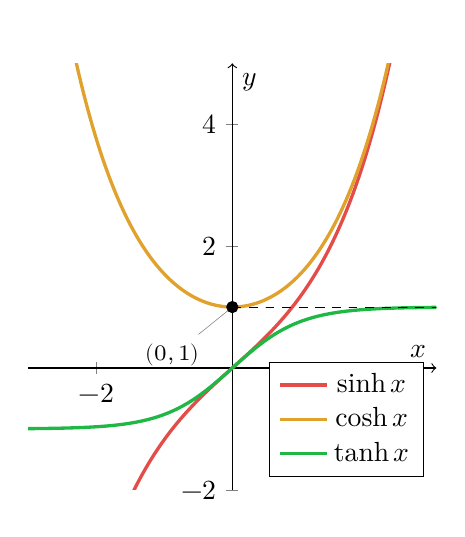
\begin{tikzpicture}
            \pgfplotsset{width = \linewidth/2+2em,height = 7cm}
            \begin{axis}[
                    axis x line = middle,
                    axis y line = middle,
                    every inner x axis line/.append style={->},
                    every inner y axis line/.append style={->},
                    title={\itshape 双曲函数},
                    legend pos = south east,
                    xlabel = $x$,
                    ylabel = $y$,
                    ymajorgrids = false,
                    xmajorgrids = false,
                    grid style = dashed,
                    samples = 1000,
                    xmin = -3, xmax = 3,
                    ymin = -2, ymax = 5
                ]
                \addplot+[
                    no marks,
                    very thick,macred!90!black
                ]{sinh(x)};

                \addplot+[
                    no marks,
                    very thick,macyellow
                ]{cosh(x)};

                \addplot+[
                    no marks,
                    very thick,macgreen!90!black
                ]{tanh(x)};

                \addplot[
                    domain = 0:10,dashed
                ]{1};

                \addplot [only marks,mark=*]
                coordinates { (0,1) };

                \node[coordinate, pin=230:{\footnotesize$(0,1)$}] at (axis cs:0,1){};
                \legend{$\sinh x$,$\cosh x$,$\tanh x$}
            \end{axis}
        \end{tikzpicture}
    }

    \begin{tikzpicture}
        \pgfplotsset{width = \linewidth ,height = 8cm}
        \begin{axis}[
                axis x line = middle,
                axis y line = middle,
                every inner x axis line/.append style={->},
                every inner y axis line/.append style={->},
                title={\itshape 反双曲函数},
                legend pos = south east,
                xlabel = $x$,
                ylabel = $y$,
                ymajorgrids = false,
                xmajorgrids = false,
                grid style = dashed,
                samples = 1000,
            ]
            \addplot+[
                no marks,
                very thick,macred!90!black
            ] table {Plot4.dat};

            \addplot+[
                no marks,
                very thick,macyellow
            ] table {Plot5.dat};

            \addplot+[
                no marks,
                very thick,macgreen!90!black
            ] table {Plot6.dat};


            \legend{$\operatorname{arcsinh}x$,$\operatorname{arccosh}x$,$\operatorname{arctanh}x$}
        \end{axis}
    \end{tikzpicture}
    \caption{反三角函数、双曲函数与反双曲函数的图像}
    \label{反三角函数、双曲函数与反双曲函数的图像}
\end{figure}


\section{“充要条件”的理解}
在部编版高中数学教材的必修一(旧版的选修2-1)中,大家已经学习了简易的逻辑术语,包括特称、全称量词,
以及充分条件、必要条件与充分必要条件的定义。但实际上,大家只有在选择填空题中才会见到它们的身影(特别是几种“条件”)%
而很少在证明题中应用到它们。下面我们就通过一些例子来更加深入的理解这几种“条件”。
\subsection{必要条件——自信的估计}
我们知道$p$是$q$的必要条件可以用$q \Rightarrow {p}$来表示,但仅有符号无法帮助我们很好地理解抽象的概念。
举一个简单的例子:\textit{“幽幽子吃东西”}是\textit{“幽幽子吃饱饭”}的必要条件。因为\textbf{不(表示否定) }\textit{“吃东西”}就一定%
\textbf{不可能(同样表示否定)}\textit{“吃饱饭”};由\textit{“幽幽子吃饱饭”}这一事实,我们就一定可以得出\textit{“幽幽子吃东西”}这一前提
条件。(即$q$:\textit{“幽幽子吃饱饭”} $\Rightarrow p$:\textit{“幽幽子吃东西”})


从更“数学”一点的角度看,我们在高中会遇到这样一类导数题——已知函数满足一定的不等条件,求参数的取值范围。
这时,“必要性探路\footnote{先取某点的函数值解出参数的一个取值范围,再证明这个取值范围是恒成立的}”往往是很常用
的方法,但它有时候也会失效。
\begin{example}
    当$x \geqslant 0$ 时,$\mathrm{e}^x+ax^2 -x \geqslant \frac{1}{2}x^3 +1$,求$a$的取值范围。
\end{example}
\begin{solve}
    本题是2020年高考全国一卷理科数学的导数大题,很明显,本题可以用分离参数的方法解出。
    但如果我们用必要性探路,会有什么后果呢?

    记
    \[
        f(x)=\mathrm{e}^x+ax^2 -x-\left (\frac{x^3}{2} +1\right )
        .\]
    容易发现$f(0)=0$,那么必须有$f'(0)\geqslant 0$,
    而$f'(x)=\mathrm e^x-\frac{3}{2}x^2+2ax-1.$,则
    $f'(0)=0$ 那么又必须有$f''(0)\geqslant 0$,而$f''(x)=\mathrm e^x-3x+2a$,则$a\geqslant -\frac{1}{2}$.

\end{solve}

然而,这并非正确的答案。事实上,利用分离参数法,我们解得$a$的取值范围为$\left [ \frac{7-\mathrm e^2}{4},+\infty  \right ) $,
在$x=2$时取得最小值。这说明“便捷”的必要性探路并非万能。究其原因,必要条件是“被扩大的前提”。在它之中,仅有一部分
能够推断出“结果”$q$,这就好比说“吃了东西的幽幽子不一定能吃饱”。

\subsection{充分条件——不一定完备的前提}
比起必要条件,充分条件理解起来似乎轻松一些。正如$p\Rightarrow q$中的右箭头一样,它的定义符合我们一般的思维
顺序——由因及果。需要注意的是,一个结果可以对应多种原因,因此,充分条件是不唯一的。

\subsection{充要条件——终极目标}
可以这么说:充要条件是数学中最精美的需要。一个命题被提出后,只有找到它的充要条件,才能说它得到了解决。


拆解充要条件的符号``$\Leftrightarrow $",我们发现它由``$\Leftarrow$" ``$\Rightarrow $"两部分组成。
这看起来像是在说废话,实际上却蕴含了这么一种思想:如果你想证明两个命题等价,只需要证明由任意一方可以推出
另外一方即可。还是像废话?我们来看一个实际的思路:如果$a,b$之间满足一定关系,证明$a=b$不仅可以由等量关系推出,也可
分别证明$a\geqslant b$,~$b\geqslant a$,从而得出$a=b$.
\begin{example}
    已知集合$A=\bigl\{\,x \bigm| x=2m-1,\,m\in \mathbb{Z} \,\bigr\}$,~$B=\bigl\{\,x \bigm| x=4k\pm 1,\,k\in \mathbb{Z} \,\bigr\} $,求证:$A=B$.
\end{example}
\begin{prove}
    一方面,若$x\in A$,则当$m=2k$时,~$x=4k-1$且$k\in \mathbb{Z}$,


    当$m=2k+1$时,$x=2(2k+1)-1=4k+1$,~$k\in \mathbb{Z}$,从而$x\in B$,即得$A\subseteq B$.


    另一方面,若$x∈B$,则$x=4k±1$,~$k\in \mathbb{Z}$.


    当$x=4k-1$时,$x=2(2k)-1$,令$m=2k\in \mathbb{Z}$,有$x=2m-1\in A$.


    当$x=4k+1=2(2k+1)-1$,令$m=2k+1\in \mathbb{Z}$,有$x=2m-1\in A$.


    从而$x\in A$,即得$B\subseteq A$,综合以上两方面即得$A=B$.
\end{prove}


我们再用一个例子简单地介绍证明“$p$是$q$的充要条件”的思路。
\begin{example}
    已知$a$,~$m$,~$n\in \mathbb{N^*}$,求证:$a^m-1\mid a^n-1$的充要条件是$m\mid n$.
\end{example}
\begin{prove}
    充分性:由$m\mid n$可设$n=km$,~$(k\in \mathbb{Z})$,我们有
    \[
        \begin{aligned}
            a^m-1=(a-1)(1+a+a^2+\dots +a^{m-1}), \\
            a^n-1=(a-1)(1+a+a^2+\dots +a^{km-1}).
        \end{aligned}
    \]
    上式可由等比数列求和公式得到。又
    \[
        \begin{aligned}
             & \mathrel{\phantom{=}} (a-1)\left( a+a^2+\dots +a^{km-1} \right)               \\
             & =  1+a+a^2+\dots +a^{m-1}+a^m+\dots+a^{2m}+\dots+a^{km-1}                     \\
             & =  (a-1)\left( 1+a+a^2+\dots +a^{m-1})(1+a^m+a^{2m}+\dots +a^{(k-1)m} \right) \\
             & =  (a^m-1)\left( 1+a^m+a^{2m}+\dots +a^{(k-1)m} \right) .
        \end{aligned}
    \]
    故$a^m-1\mid a^n-1$.充分性得证


    必要性:设 $a^m=t$,则$a^n=(a^m)^{\frac{n}{m}}=t^{\frac{n}{m}}$.由
    \[
        t^{\frac{n}{m}}-1=(t-1)\left( 1+t+t^2+\dots +t^{\frac{n}{m}-1} \right)
        .\]
    是整数且$t-1\mid t^{\frac{n}{m}}-1$可知
    $\frac{n}{m}$是整数,由此$m\mid n$得证.


    综上所述,$a^m-1\mid a^n-1$的充要条件是$m\mid n$.

\end{prove}

上面这个例子向我们展示了证明充要性的基本方式:分别证明充分性和必要性。很多情况下,某一方面的证明需要利用
反证法,而且两个方面的证明思路互相提示。

\section{常用方法——放缩、夹逼与归纳}
\subsection{放缩法}
进入高等数学的学习之后,我们不会再像高中那样特意地证明一些不等式。但在证明某些命题,或者求极限的时候,仍需要
证明不等式,这个时候放缩法的使用就显得尤为重要。这一节,我们会针对高等数学(数学分析)的学习需要,介绍一些常
用的放缩技巧和思路。
\subsubsection{放缩的常用工具}


\begin{itemize}
    \item \textbf{与绝对值有关的不等式}

          关于绝对值,我们熟知有以下不等式:
          \[
              \big | \lvert a \rvert-\lvert b\rvert  \big |
              \leqslant \lvert a\pm b\rvert \leqslant \lvert a\rvert +\lvert b\rvert
              .\]

          $a$,~$b$间取加号时,左边等号的成立条件是$a$,~$b$异号,右边等号的成立条件是$a$,~$b$同号。取减号是恰好相反。

          在之后证明收敛数列极限唯一、极限乘法规则和柯西审敛准则时,都会用到这一工具。
          \begin{example}
              求证:若$\lim\limits_{n \to \infty} a_n =a$,则$\lim\limits_{n \to \infty} |a_n| =|a|$.
          \end{example}
          \begin{prove}
              由已知,对于任意正数$\varepsilon$,总存在正整数$N$,使得当$n>N$时,总有$|a_n-a|<\varepsilon$.


              由绝对值不等式,当$n>N$时,总有$\big ||a_n|-|a|\big |\leqslant |a_n-a|<\varepsilon$.
              因此$\lim\limits_{n \to \infty} |a_n| =|a|$.
          \end{prove}
          另外,对于任意$n$个数,上述不等式还有拓展:
          \[
              |\;\!a_1+a_2+\cdots +a_n|\leqslant |a_1|+|a_2|+\cdots +|a_n|
              .\]

          取等条件为$a_1,\,\dots\,,a_n$全部同号。
    \item \textbf{与三角函数有关的不等式}

          我们可以通过几何方法证明:
          \[
              \sin x<x<\tan x,\quad\left( 0<x<\frac{\symup\pi}{2} \right)
              .\]

          具体过程可以参照%加文献引用
          各类高数或数分教材。然而,在刚接触高数时,我们往往不需要用到这么精细的放缩。注意到正弦和余弦函数的绝对值均不大于 $1$,利用
          这一性质就可以解决很多问题了。

    \item \textbf{与指对数有关的不等式}

          我们知道$\lim\limits_{n \to \infty}\left (1+\frac{1}{n}\right )^n=\mathrm e$.事实上,
          数列$\left\{ \left (1+\frac{1}{n}\right )^n  \right\} $是递增的,证明过程如下:
          \begin{prove}
              由均值不等式,
              \begin{equation}
                  \left (1+\frac{1}{n}\right )^n=1\cdot \left (\frac{n+1}{n}\right )\left (\frac{n+1}{n}\right )
                  \cdots \left (\frac{n+1}{n}\right )<
                  \left (\frac{1+n\cdot \frac{n+1}{n}}{n}\right )^{n+1}=\left (1+\frac{1}{n+1}\right )^{n+1}\label{与指对数有关的不等式}
              \end{equation}
          \end{prove}


          另外,我们还可以证明 $\lim\limits_{n \to \infty}\left (1+\frac{1}{n}\right )^{n+1}=\mathrm e$,且数列
          $\left\{  \left (1+\frac{1}{n}\right )^{n+1} \right\}  $是递减的。结合以上事实,我们得到:
          \[
              \left (1+\frac{1}{n}\right )^n<\mathrm e<\left (1+\frac{1}{n}\right )^{n+1\!\!\!\!\!\!\!\!\!\!\!\!}
              ,\]


          取对数后,我们得到一个很有用的结论:
          \[
              \frac{1}{n+1}<\ln \left( 1+\frac{1}{n} \right) <\frac{1}{n}, \quad (n\in \mathbb{N} ).
          \]


          我们在高中时利用导数工具得到过这个结论,事实上,在正整数范围内,它可以仅由数列极限的知识得到。

    \item \textbf{与阶乘有关的不等式}

          阶乘有许多重要的性质,这里我们只介绍在不等关系方面的性质。

          可以这么说,阶乘是比常数的指数更“大”的存在,见     下面的例子。
          \begin{example}
              求证:$\lim\limits_{n \to \infty} \frac{n!}{2^n} =0$.
          \end{example}
          \begin{prove}
              \[
                  \frac{n!}{2^n}=\frac{2\times 2\times \cdots\times 2}{1\times 2\times \cdots\times n}
                  <2\cdot \frac{2}{n}=\frac{4}{n}
                  .\]

              余略。
          \end{prove}


          \begin{example}
              求证:对$n\in \mathbb{N}$,$n!>\left (\frac{n}{\mathrm e} \right )^n$.\label{例子9}
          \end{example}
          \begin{prove}
              我们取数列$a_n=\left (\frac{n}{\mathrm e} \right )^n$,则
              \begin{gather}
                  \frac{a_n}{a_{n-1}}=\frac{n^n}{(n-1)^{n-1}\mathrm e}=\frac{n\left (1+\frac{1}{n-1}\right )^{n-1}}{\mathrm e},\\
                  a_n=\frac{a_n}{a_{n-1}} \frac{a_{n-1}}{a_{n-2}}\cdots \frac{a_2}{a_1} a_1< n(n-1)\cdots 2a_1<n(n-1)\cdot \cdots \cdot 2\cdot 1=n!.
              \end{gather}
              证毕。
          \end{prove}

          例 \autoref{例子9} 揭示了$n$的阶乘与$n$的$n$次幂之间的关系,它与重要极限$\lim\limits_{n \to \infty}\left (1
              +\frac{1}{n}\right )^n=\mathrm e$密切相关。事实上,我们有极限
          $\lim\limits_{n \to \infty}\frac{n}{\sqrt[n]{n!}}=\mathrm e$.
\end{itemize}

\subsubsection{放缩的常用手段}
\label{sssec:A}
许多时候,面对一些形式复杂的式子,我们一时想不到如何对其进行放缩。下面我们将用几个例子介绍放缩的常用手段。

\paragraph{朝着可以化简的方向放缩}

要证明某些累加式或累乘式的值在某个范围内,我们一般把舍弃某些项,把它们放缩成可以求和或求积的形式。
\begin{example}
    求证:$\left ( 1+\frac{1}{2}\right )\left ( 1+\frac{1}{2^2}\right )
        \cdots \left ( 1+\frac{1}{2^n}\right )<\mathrm{e}$.
\end{example}
\begin{prove}
    由 \eqref{与指对数有关的不等式} 的最后一个结论,我们有$\ln \left ( 1+\frac{1}{2^k}\right )<\frac{1}{2^k}(k=1,2,\cdots,n)$.则
    \[
        \ln\left( \left ( 1+\frac{1}{2}\right )\left ( 1+\frac{1}{2^2}\right )
        \cdots \left ( 1+\frac{1}{2^n}\right ) \right) <\frac{1}{2}+\frac{1}{2^2}
        +\cdots+\frac{1}{2^n}=\frac{1}{2}\cdot \frac{1-\frac{1}{2^n}}{1-\frac{1}{2}}<1
        .\]
    从而$\left ( 1+\frac{1}{2}\right )\left ( 1+\frac{1}{2^2}\right )
        \cdots \left ( 1+\frac{1}{2^n}\right )<\mathrm{e}$.
\end{prove}


上面的例子中,我们观察到待证式左边暗含等比数列,就想办法将其提取出来。
恰好,取对数之后放缩可以把“$1$”消去,便完成了化简的工作。

\paragraph{待定系数,先猜后证}

某些不等式,特别是证明某式子大于或小于某个非0常数,(这在求极限时很常见)可以用待定系数的方法来进行放缩。
\begin{example}
    求证:$\lim\limits_{n \to \infty}\sqrt[n]{n}=1.$
\end{example}
\begin{prove}
    下面我们将会用到3.2节会学到的夹逼定理——事实上,我们的目标是证明$\sqrt[n]{n}-1$小于
    一个极限为$0$的数列。观察到$\sqrt[n]{n}-1$的特点,我们发现移去$1$对原式取$n$次方后可以实现
    有效的化简。


    令$\sqrt[n]{n}=1+\lambda_n$,则
    \[
        n=(1+\lambda_n)^n=1+n\lambda_n+\frac{n(n-1)}{2}\lambda^2 _n+\cdots >1+\frac{n(n-1)}{2}\lambda^2 _n
        .\]
    由此解得$\lambda_n<\sqrt{\frac{2}{n}}$,因此$0<\sqrt[n]{n}-1<\sqrt{\frac{2}{n}}$.由夹逼
    定理可知$\lim\limits_{n \to \infty}\sqrt[n]{n}=1.$
\end{prove}


关于这种技巧,在初等数学的范围内也有很多应用,例如用均值不等式、柯西不等式等解题时,利用取等条件限制,
解出配凑的系数。类似的例子还有很多,限于篇幅,就不在此处赘述了。


总之,放缩法的技巧和工具五花八门。只有勤加练习,多积累有关知识,才能得心应手地应用。然而,我们
也没有必要像高中时那样,为了应试,而刻意去寻找各种偏、怪的不等式,掌握常用且有用的那部分即可。
% \end{enumerate}



\subsection{夹逼定理}
在几乎所有高数教材中,我们都会看到这样一条定理:若数列$\{ b_n \} $和$\{ c_n \} $都收敛于$a$,且对
所有充分大的$n$,有$b_n \leqslant a_n \leqslant c_n$,则数列$\{ a_n \} $也收敛,且极限也为$a$.这就是有名的夹逼定理。


关于夹逼定理的证明,请参照各种教材。我们之所以在此特别提到夹逼定理,是因为其背后蕴含着一个重要思想——夹逼思想,即
“从两边往中间靠”。事实上,这一思想贯穿我们的数学学习历程。
\begin{example}
    已知函数$f(x)=ax^2+bx+c$的图像过点$(-1,0)$,且对$x\in \mathbb{R}$都有$4x-12\leqslant f(x)\leqslant 2x^2-8x+6$.求$f(x)$.
\end{example}
\begin{solve}
    这道题节选自$2021$年广东省中考数学卷$25$题,其关键一步就利用了夹逼思想。


    当$x=3$时,$4x-12=2x^2-8x+6=0$,则$f(3)=0$,即$f(x)=a(x+1)(x-3)=ax^2-2ax-3a$.


    又$4x-12\leqslant f(x)$,则$ax^2-(2a+4)x+12-3a\geqslant 0$,即
    \[
        \Delta = (2a+4)^2-4a(12-3a)=16a^2-32a+16=0
        .\]
    解得$a=1$.


    从而 $f(x)=x^2-2x-3$.
\end{solve}
无论是初等的不等式问题,还是高等的求极限,夹逼思想都非常重要。其思路也类似于放缩的基本手段——用可直接求极限的
式子,去“夹”出不那么容易直接求出极限的式子。总而言之,就是由未知联想已知,再由已知导出未知。下面的例子就是
夹逼定理在求极限中的经典应用。
\begin{example}
    求$\lim\limits_{n \to \infty}\left( \frac{1}{\sqrt{n^2+1}}+\frac{1}{\sqrt{n^2+2}}+\cdots +\frac{1}{\sqrt{n^2+n}} \right) .$
\end{example}
\begin{solve}
    注意到
    \[
        \frac{n}{\sqrt{n^2+n}}\leqslant \frac{1}{\sqrt{n^2+1}}+\frac{1}{\sqrt{n^2+2}}+\cdots +\frac{1}{\sqrt{n^2+n}}
        \leqslant \frac{n}{\sqrt{n^2+1}}
        .\]
    而
    \[
        \lim\limits_{n \to \infty}\frac{n}{\sqrt{n^2+n}}=\lim\limits_{n \to \infty}\frac{1}{\sqrt{1+\frac{1}{n}}}=1,\quad
        \lim\limits_{n \to \infty}\frac{n}{\sqrt{n^2+1}}=\lim\limits_{n \to \infty}\frac{1}{\sqrt{1+\frac{1}{n^2}}}=1
        .\]
    由夹逼定理即得$\lim\limits_{n \to \infty}\left( \frac{1}{\sqrt{n^2+1}}+\frac{1}{\sqrt{n^2+2}}+\cdots +\frac{1}{\sqrt{n^2+n}} \right) =1$.
\end{solve}
% \def\thesubsubsection{\arabic{subsubsection}}
上面的例子也用到了 \autoref{sssec:A} 提到的放缩手段——朝着可以化简的方向放缩。
\subsection{数学归纳法}
在高中时,我们已经对数学归纳法有所了解,但并没有深入地研究其应用,并且仅局限于常见的第一数学归纳法。下面我们更深入地介绍一下
数学归纳法的奇妙之用。
\subsubsection{第一数学归纳法}
第一数学归纳法,顾名思义,就是我们最常用的归纳法。其具体内容就不在此处展开,我们通过一个例子来帮助大家回忆一下它的使用。
\begin{example}
    设$a_n=\sqrt{2+\sqrt{2+\sqrt{2+\cdots}}}$($n$重根式),求证$\lim\limits_{n \to \infty}a_n$存在并求其极限。
\end{example}
\begin{solve}
    $a_n$满足递推关系:$a_1=\sqrt{2}$, $a_{n+1}=\sqrt{a_n+2}$.

    注意到$a_2=\sqrt{2+\sqrt{2}}>a_1$, $a_3=\sqrt{2+\sqrt{2+\sqrt{2}}}>a_2$.

    我们猜想,如果$a_n>a_{n-1}$,那么
    \[
        a_{n+1}-a_n=\sqrt{a_n+2}-\sqrt{a_{n-1}+2}=
        \frac{a_n-a_{n-1}}{\sqrt{a_n+2}+\sqrt{a_{n-1}+2}}>0
        .\]
    从而$a_{n+1}>a_n$,由数学归纳法可得$\{ a_n\}$单调递增。


    同样由数学归纳法可以证得$a_n<2$,因此$\{ a_n\}$单调递增有上界,则$\{ a_n\}$收敛。设其极限为$a$,在递推式两边取极限
    可以解得$a=2$(负值舍去),从而$\lim\limits_{n \to \infty}a_n=2$.
\end{solve}
这个例子中,我们两次运用数学归纳法证明了很“显然”,却不方便用常规方法证明的结论,可见其作用强大。
\subsubsection{第二数学归纳法}
第二数学归纳法与第一数学归纳法类似,但却比它更强,其内容如下:

\begin{enumerate}
    \item 前提:当$n=m$,~$(m \in \mathbb{N})$时,结论成立;
    \item 假设与归纳:假设$n\leqslant k$(注意与第一数学归纳法比较)时结论成立,若由此推得$n=k+1$时结论也成立,
          则结论对$n \geqslant m$总成立。

\end{enumerate}

我们可以利用高中数学教材中多米诺骨牌的例子来理解:第一数学归纳法是“前一块骨牌倒下”推出“后一块骨牌倒下”,
而第二数学归纳法是“前面所有的骨牌倒下”推出“后一块骨牌倒下”,它同样是合理的。


\begin{example}
    【\textup{Chebyshev}(切比雪夫)多项式】求证:$\cos n\theta$,~$(n \in \mathbb{N})$可以表示为关于$\cos \theta$的整系数多项式。
\end{example}
\begin{prove}
    首先理解题干意思:我们要将$\cos n\theta$的
    展开式写成$a_0+a_1\cos \theta+a_2\cos^2 \theta+\cdots +a_n \cos^n\theta$的形式,其中$a_k$均为整数。


    我们考虑积化和差公式(见 \autoref{积化和差} ),有$2\cos k\theta\cos \theta=\cos (k+1)\theta +\cos (k-1)\theta$.
    显然$n=1$,~$2$时$\cos n\theta$,~$(n \in \mathbb{N})$均可以表示为关于$\cos \theta$的整系数多项式\footnote{$n=2$时即二倍角公式。}。
    假设$n\leqslant k$时$\cos n\theta$均可以表示为关于$\cos \theta$的整系数多项式,则
    \[
        \cos (k+1)\theta=2\cos k\theta\cos \theta-\cos (k-1)\theta
        .\]
    是整系数多项式的减法运算,故$\cos (k+1)\theta$仍为整系数多项式,由第二数学归纳法知结论成立。
\end{prove}
仔细体会上面的证明过程,你会渐渐认识到数学归纳法的强大威力。

\section{参数方程与坐标系补充}
\subsection{参数方程简介}
平面直角坐标系上的参数方程,就是分别用参量$t$定义坐标分量$x,y$,$x,y$之间通过$t$形成某种关系
(很多时候可以统一到一个方程里),并在坐标系上体现为曲线。简而言之,参数方程是曲线方程(函数图像)的一种形式。
\begin{example}
    $ x=r\cos \theta$,~$y=r\sin \theta$是圆的参数方程,可以化为圆的标准方程$x^2+y^2=r^2.$
\end{example}
\begin{example}
    $ x=a\cos \theta$,~$y=b\sin \theta$ 是椭圆的参数方程,可以化为椭圆的标准方程
    $\displaystyle \frac{x^2}{a^2}+\frac{y^2}{b^2}=1.$
\end{example}
\begin{example}\label{li18}
    滚轮线是匀速直线运动和匀速圆周运动的叠加运动的轨迹。一个半径为$r$刚体圆形滚轮沿直线往前滚动$\theta$角时,质心前进的距离是 $r\theta $,
    高度保持为$r$ 不变,其初始坐标记作 $(0,r)$. 设$\theta =0$时轮沿上某点$P$接触地面,其坐标为$(0,0)$. 则滚动 $\theta$ 角后,
    $P$ 点的运动 即质心匀速直线运动与$P$ 点相对质心匀速圆周运动的线性叠加,满足:
    $(x,y) = (r\theta ,r) + (-r\sin \theta,-r\cos \theta) = \bigl(r(θ - \sin θ),r(1 - \cos θ)\bigr)$.这样就得出一个$x,y$关于
    参数$\theta $的参数方程,称为滚轮线或摆线。

    \begin{center}
        \begin{tikzpicture}
            \pgfplotsset{width=14cm,height=7cm}
            \begin{axis}[
                    title={当 $r=1$ 时的摆线},
                    xmin = -2, xmax = 7 ,
                    ymin = -2, ymax = 4.5,
                    axis x line=middle,
                    axis y line=middle,
                    every inner x axis line/.append style={->},
                    every inner y axis line/.append style={->},
                    xlabel=$x$,
                    ylabel=$y$,
                ]
                \addplot [
                    variable = t,
                    domain = 0 : 2*pi,
                    very thick,
                    trig format plots = rad,
                    samples = 1000,
                ] (
                {t - sin(t)},
                {1 - cos(t)}
                );
            \end{axis}
        \end{tikzpicture}
    \end{center}
\end{example}
事实上,并非所有参数方程都可以简单地消去参数,转化为关于$x$,~$y$的方程。(如例 \autoref{li18} 中的滚轮线)但它们仍可以进行求切线斜率等操作。


\subsection{极坐标、柱坐标与球坐标}
\subsubsection{极坐标系}
极坐标系由一个原点——极点,和以极点为端点的一条射线——极轴构成。
与我们熟知的平面直角坐标系类似,极坐标系也包含两个坐标分量:与极点的距离——极径$\rho $,
以及与极轴正方向的夹角——极角$\theta $,
其中$\rho $都只能取非负值,而$\theta $可以取任意实数值,且每增加$2\symup\pi$,就相当于绕极点“转了一圈”。


容易发现,极坐标与直角坐标有转换关系如下:
\[
    \rho ^2=x^2+y^2,\quad\rho \cos \theta=x,\quad\rho \sin \theta=y
    .\]


对于一些更“对称”的曲线来说,用极坐标描述它们,比用直角坐标系简单便捷得多。
\begin{example}
    以圆锥曲线的一个焦点(椭圆取左焦点,双曲线取右焦点)为极点,以过焦点的对称轴为极轴(向右为正方向)
    ,其极坐标方程可以表示为
    \[
        \rho =\frac{ep}{1-e\cos \theta},\quad(0\leqslant \theta < 2 \symup\pi)
        .\]
    其中$e$为圆锥曲线的离心率,$p$为焦准距。
\end{example}


这一极坐标方程暗含圆锥曲线的统一定义,足见极坐标系的优势所在,其推导过程请读者自行尝试。%....
\begin{example}
    心形线$\rho =1-\cos \theta$,~$ (0\leqslant \theta < 2 \symup\pi)$若改写为直角方程,其表达式将变为
    $(x^2+y^2+x)^2=x^2+y^2$,不够直观。
\end{example}

\begin{center}
    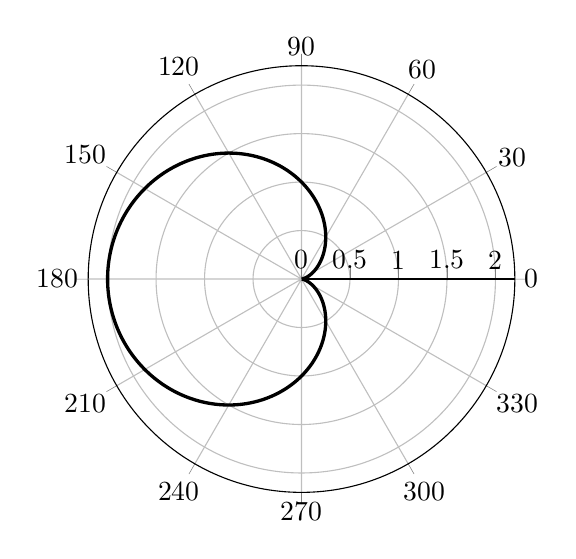
\begin{tikzpicture}
        \pgfplotsset{width=7cm,height=7cm}
        \begin{polaraxis}
            \addplot [
            samples = 400,
            domain = 0:2*pi,
            very thick,
            trig format plots = rad,
            ] (deg(x), {1 - cos(x)});
        \end{polaraxis}
    \end{tikzpicture}
\end{center}

以上两个例子向我们展示了极坐标系适用的几个场景。此外,阿基米德螺线,玫瑰线等
都是极坐标的典型例子。

\begin{center}
    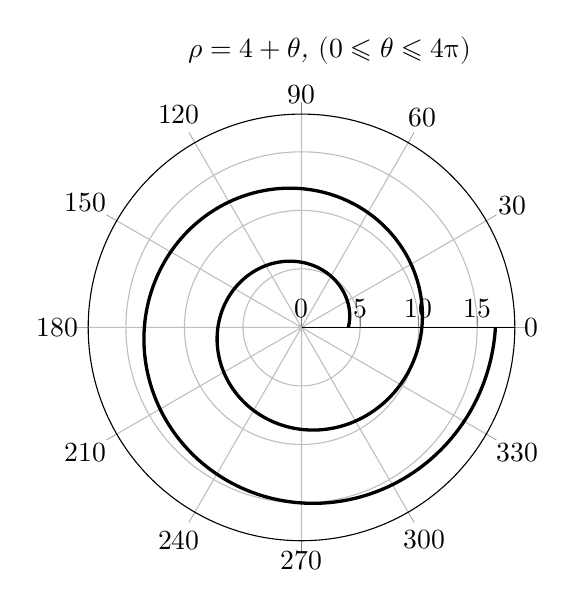
\begin{tikzpicture}
        \pgfplotsset{width=7cm,height=7cm}
        \begin{polaraxis}[title = {\itshape 阿基米德螺线 $\rho =4+\theta$,~$(0\leqslant \theta\leqslant 4\symup \pi )$}]
            \addplot [
            samples = 400,
            domain = 0:4*pi,
            very thick,
            trig format plots = rad,
            ] (deg(x), {4 + x});
        \end{polaraxis}
    \end{tikzpicture}
    \quad
    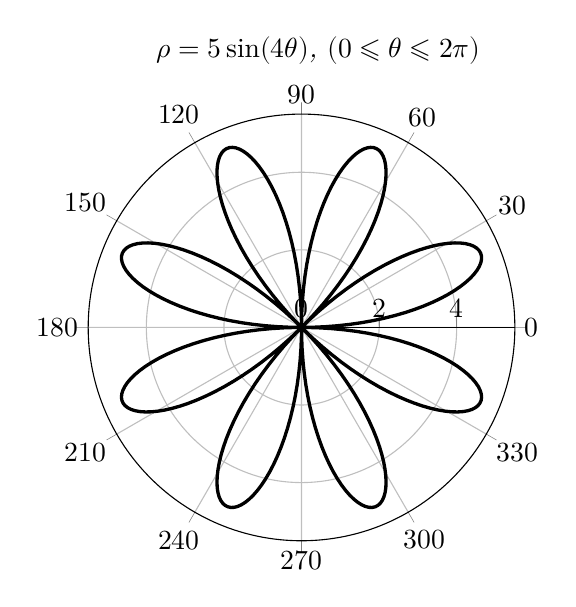
\begin{tikzpicture}
        \pgfplotsset{width=7cm,height=7cm}
        \begin{polaraxis}[title = {\itshape 玫瑰线 $\rho =5\sin (4\theta)$,~$(0\leqslant \theta\leqslant 2\pi )$}]
            \addplot [
            samples = 400,
            domain = 0:2*pi,
            very thick,
            trig format plots = rad,
            ] (deg(x), {5*sin(4*x)});
        \end{polaraxis}
    \end{tikzpicture}
\end{center}

\subsubsection{柱坐标与球坐标简介}
柱坐标可以看作在极坐标系平面上,再“拉”出一条垂直的$z$轴。我们熟知的等距螺线就可以方便地用它来表示。

球坐标系是极坐标系在空间中的延伸。它有两个角分量:连线与正$z$轴(垂直轴)的夹角——天顶角$\theta$,以及
连线在$xy$平面的投影与正$x$轴的夹角——方位角$\phi$.它在研究球对称的情况时十分便捷。
\section{极限思维与实数理论概述}
高中时有位数学老师的话让我印象深刻:“没学过微积分,人半辈子都是黑暗的哦。”这种看法虽然比较极端,但也暗示
了微积分对人思维的重要性。其中,最重要的一点,就是如何用精确的数学语言去描述看似浅显的“极限”“连续”概念。

\subsection{从定义看极限}\label{continous property}
高数课本上重点阐述了关于数列极限的“$\varepsilon  \text{-} N$语言”和关于函数极限的“$\varepsilon  \text{-} \delta$语言”,
这里我们重点从数列极限的角度切入,帮助大家弄懂极限是什么,要怎么证明有关收敛性的题目。


仔细观察$\varepsilon  \text{-}N$语言的内容:若对于所有正数$\varepsilon$,均存在正整数$N$,使得对于所有大于$N$
的整数$n$,都有$|\;\!a_n-a|<\varepsilon$.记住$\varepsilon$是可以\textbf{任意}小的,只要它比0大,取
什么值都没问题。但我们的$|a_n-a|$居然比它还要小!也就是说,只要有无穷多个(可以说明,这等价于“存在正整数$N$,使得对于所有大于$N$
的整数$n$”)$|\,a_n-a\,|$比任意小的$\varepsilon$还要小,就可以说$a_n$收敛于$a$.


这样,我们就用自然语言描述了极限的意思——无论多小,总还存在更小的。需要注意的是,这种描述有道理,但并不完全
准确。而下面我们就来介绍如何准确地理解和应用极限的定义。
\begin{example}
    求证:若$a_n>0$,且 $\lim\limits_{n \to \infty}\frac{a_n}{a_{n+1}}=l>1$,则 $\lim\limits_{n \to \infty}a_n=0$.
\end{example}
\begin{prove}
    题设等价于$\lim\limits_{n \to \infty}\frac{a_{n+1}}{a_n}=\frac{1}{l}=t<1$,
    即
    \[
        \forall \varepsilon>0,\,\exists N\in \mathbb{N},\,\forall n>N,\,\left|\, \frac{a_{n+1}}{a_n}-t\, \right| <\varepsilon
        \Rightarrow \frac{a_{n+1}}{a_n}<t+\varepsilon
        .\]
    我们取$\varepsilon=1-t-\tau $,其中$\tau >0$且$\tau +t<1$.即得$\frac{a_{n+1}}{a_n}<1-\tau $.
    因此,$\forall n>N,$
    \[
        a_n=a_{N+1}\frac{a_{N+2}}{a_{N+1}}\cdots \frac{a_n}{a_{n-1}}<a_{N+1}(1-\tau)^{n-N-1}
        .\]
    对于任意正数$\delta$,我们取$n>\left\lfloor\log_{1-\tau}\frac{\delta}{\scriptstyle{a}_{{N+1}}}  \right\rfloor+N+2$,则有
    \[
        a_n<a_{N+1}(1-\tau)^{\left\lfloor \log_{1-\tau}(\delta / a_{N+1}) \right\rfloor+1}
        <a_{N+1}(1-\tau)^{\log_{1-\tau}(\delta / a_{N+1})}=\delta
        .\]
    又$a_n>0$,从而$\lim\limits_{n \to \infty}a_n=0$.
\end{prove}
上面的例子中,我们直观地感觉到$a_n$类似于“公比小于1的等比数列”,再利用极限的定义,构造放缩得到“等比数列”。
从始至终,极限的定义都得到了应用。


无论如何,最基本的定义或定理都是许多题目的关键,熟练掌握的重要性不言而喻。

\subsection{实数完备性的理解}
我们知道,数的概念发展经历了由自然数到整数,再到有理数,最后到实数和复数的过程。其中,有理数与实数
的辨析是这一节内容的重点。


我们知道,一个数是有理数的充要条件是,它可以被表示为$\frac{q}{p}$的形式,其中$p$,~$q$是互质(最大公因数为1)
的整数。我们说有理数是稠密的,是指任意两个实数之间必存在有理数。(利用前述的放缩法可以证明,这作为一道小小
的思考题)


但它并不是连续(参照 \autoref{continous property} 关于连续性的定义)的,因为任意两个有理数之间必存在无理数(事实上,
对任意有理数$a$,~$b$,取$c=a+\frac{1}{\sqrt{2}}(b-a)$即可)。这说明有理数并不“完美”,直观上来说,
仅由有理数并不能生成一条连续的数轴,只能得到一系列离散的点——有理数与有理数之间是有“空隙”的。


而引入实数的概念后,连续性的问题得到了解决。我们是这样阐述实数的连续性的:对于集合$X,Y$,若$\forall x\in X
$,~$y\in Y$,~$x\leqslant y$,则$\exists c\in \mathbb{R}$,~$x\leqslant c\leqslant y$.可以这么说,无论两个实数多么“接近”,总有那么一个
实数可以“插入”到它们中间,这就是所谓“连续不断”。
\begin{example}
    取集合$X=\{\, x\mid x^2\leqslant 2\,\}$,~$Y=\{\, y\mid y^2>2\,\}$,显然满足$\forall x\in X,\,y\in Y$,~$x\leqslant y$.
    而$\exists ! c\in \mathbb{R}$,~$c^2=2$,~$x\leqslant c\leqslant y$.如果限制在有理数范围内,则无法找到这样的$c$.
\end{example}


上面几段文字的描述可能显得很抽象。但不要紧,多去找一些实例或推论,尝试自己去证明一些结论,理解必然会不断加深。
具体可以查询有关“实数完备性等价定理”的资料。

\chapter[宇佐见堇子的 \LaTeX 之旅]{宇佐见堇子的 \LaTeX 之旅}
\label{cp:宇佐见堇子的 LaTeX 之旅}
\addauthor{小飞舞}
\begin{center}
    \begin{tcolorbox}[colback=black!15!white,%gray background
            colframe=black!80,% black frame colour
            width=15cm,% Use 5cm total width,
            arc=2mm, auto outer arc,
            boxrule=0.5pt,
            title=前言,
            fontupper = \itshape,
            % code before = {\setlength{\parindent}{2em}}
        ]
        话说那宇佐见堇子考入了东京大学第一年就做出了相当成功的研究,正在她想把自己的想法发表在网络上的时候,她犹豫了。

        用什么组织自己的文章呢?她想。在东深见高中上学的时候,自己就曾经用 Blog 的形式将幻想乡的一些讯息扩散出去——虽然总是被当成都市传说,但也是的的确确可以在自己的电脑上随意部署样式。但现在不一样了,既然是专业性的论文,那在自己的 Blog 上部署也太看不起自己了——好歹要传到专业性的期刊上去!要不然实在太枉费自己了。

        \url{http://arxiv.org/}

        这样一个网站,上面收集了很多关于物理、数学。计算机科学等学科的论文。虽然看上去平平无奇,但的确有些非常厉害的数学家在上面发表极具影响力作品的历史\footnote{比如格里戈里·雅柯夫列维奇·佩雷尔曼 (Grigori Yakovlevich Perelman) 在 2002 年 11 月发表的解决几何化猜想 (Geometrization conjecture) 的论文。}。她当即决定就这个了。不过她在查找资料的时候注意到了要是用 \TeX 格式发表自己论文的事情,这让她非常疑惑——不是只要写出来就行吗?还管那么多格式干嘛?

        于是她找到了同样在东京大学任副教授的宇佐见莲子……
    \end{tcolorbox}
\end{center}


“呃……当时也差不多就是在那种情况下学习 \LaTeX 的,不过我倒觉得这玩意蛮重要的。”宇佐见莲子对面前的年轻学生说道。“后来……由于工作的需要,需要使用 \LaTeX 的方面也变多了——其实不只是像我这样的物理人,我觉得只要是理科都有可能会接触到 \LaTeX 的。”

“啊其实就是说……这玩意看上去高级,但是听说不太好学,呃……”上了大学后,宇佐见堇子明显稳重了许多,也不再穿她那非主流的服装了。此时她看起来和正常的学生毫无二致。

除了她在大一就已经有了成果之外。

“其实并不是这样……大多数人一开始学 \LaTeX 是为了排版自己的论文,如果只是做到这样的话学习并不算难……当然你也可以用她来排版些奇奇怪怪的东西。”宇佐见莲子说道,她轻轻撩了撩头发,“反正现在时间还早,我就先说说关于 \LaTeX 有趣的事情吧。”

“啊?你不帮我排版吗?”

“自己排啦~反正学会这个之后也是有利无害。”

\section{什么是 \LaTeX}

“\TeX 是高德纳 (Donald E. Knuth) 为排版文字和数学公式而开发的软件。当时他正在想办法出版他的巨作《计算机程序设计艺术》的前三卷,但作为“艺术”类的作品,高德纳实在无法忍受当时的排版质量——那时是 1977 年,与我们现在相差非常大的年份。\TeX 大约在 1989 年开发到一个在当时比较完善的地位,然后—— Leslie Lamport 博士在此基础上开发了 \LaTeX,实际上就是一组用 \TeX 语言的宏,那时候就大概是上世纪八十年代处左右吧。”

“那时候的人们都那么勇吗?为了排版直接写引擎?”宇佐见堇子脸上写满了惊讶。

“你要知道《计算机程序设计艺术》是多么宏伟的巨作——这玩意花费了高德纳将近一生的时光,直到现在还没写完。”宇佐见莲子摆起认真相。

“\LaTeX 相比 \TeX 有很多优势——比如在 1994 年后,\LaTeXe{} 已经完善,这玩意已经逐步称为国际上排版数学、物理、计算机等科技领域专业出版物的标准。而 \LaTeX 比 \TeX 本身更容易使用——高德纳开发 \TeX 本质是只为了自己的鸿篇巨制,而 \LaTeX 在此基础上定义了一些宏和格式,其实就将部分排版细节隐藏起来,相对而言更容易点——对你这种只想排论文的再好不过了。当然,你也可以拿 \LaTeX 来写笔记,看起来会比手写的要美观很多……一言以蔽之:


\begin{itemize}
    \item \LaTeX 具有专业的排版输出能力,本身就是为了美观而服务的。
    \item \LaTeX 目前仍是最强大的公式排版系统之一。
    \item 这玩意可以让用户更专注与内容、而不是被错综复杂的版式耍的团团转。
    \item 有很多面向 \LaTeX 开发的宏包可以解决各式各样的问题。
    \item 横跨全平台,而且开源免费。
\end{itemize}

“看起来感觉还不错。”宇佐见堇子舔了舔嘴唇。

“我们先从看得见的地方开始说起吧:首先就是这玩意的下载以及安装。”

\subsection{\LaTeX 的下载与安装}

\LaTeX 有很多发行版,比如 \verb"TeXlive", \verb"MiKTeX", \verb"MacTeX" 这些,每个发行版可能有不同的宏包管理器( \LaTeX 很多实现都是要依赖宏包才比较好搞),在这里我推荐的是比较全的 \verb"TeXlive" ,因为我用的就是 \verb"TeXlive" ,所以以下的教程全部以 \verb"TeXlive" 为基准。同样的,以下的教程基于 Windows 10。

我们仅仅需要打开 \verb"TeXlive" 的相关网站 \link{https://tug.org/texlive/},然后选择

\begin{center}
    \vbox{\textbf{\sffamily All the ways to acquire TeX Live:} $\longrightarrow$ {\sffamily on DVD}

        $\longrightarrow$ {\sffamily downloading the TeX Live ISO image and burning your own DVD}

        $\longrightarrow$ {\sffamily download from a nearby CTAN mirror}}
\end{center}

然后下载 \verb"texlive2022.iso"\footnote{根据年份不同可能会发生改变。} 即可。当然如果嫌慢,也可以使用一些镜像源:

\begin{itemize}
    \item \url{https://mirrors.nju.edu.cn/CTAN/systems/texlive/Images/}
    \item \url{https://mirrors.tuna.tsinghua.edu.cn/CTAN/systems/texlive/Images/}
    \item \url{https://mirrors.aliyun.com/CTAN/systems/texlive/Images/}
    \item \url{https://mirrors.sjtug.sjtu.edu.cn/ctan/systems/texlive/Images/}
\end{itemize}

反正各大学校一般都会有自己的镜像源,一样下载即可。

下载完成后可以运行 \verb"install-tl-windows.bat" 进行安装,选项默认就行,静待安装完成。

“呃……这个 ISO 文件怎么处理啊?”宇佐见堇子挠了挠头。

“直接解压就行了,里面就有一个 \verb"install-tl-windows.bat"。”

``什么? 你说你用的是Mac啊\dots

那就更方便了。

我们仅仅需要打开 \verb"MacTeX" 的相关网站 \link{https://tug.org/mactex/index.html},然后选择

\begin{center} \vbox{\textbf{\sffamily MacTeX Download}
$\longrightarrow$ {\sffamily MacTeX.pkg}
\end{center}

现在应该已经开始下载了。

下载完成后双击安装就行。''



\subsection{\LaTeX 的初步使用}

“安装完你的电脑里就有这么一个叫做 \LaTeX 的东西了,然后打开你的 Windows 菜单,应该会有一个 \verb"TeX live" 文件夹,里面有一个 \verb"TeXworks editor" 的软件,这是 \verb"TeXlive" 自带的一个 \LaTeX 代码编辑器。

如果是Mac,按下键盘上的F4进入启动台。你可以在里面找到一个名字叫 \verb"TeX" 的文件夹,里面有一个 \verb"TeXShop" 的软件。同样地,这也是 \verb"MacTeX" 自带的一个 \LaTeX 代码编辑器。

在里面可以写代码:

\begin{lstlisting}
    \documentclass{article}
    \begin{document}
    The quick brown fox jumps over the lazy dog.
    % use '%' to set single-line comments
    \end{document}
\end{lstlisting}

然后在左上角复选框(Mac是窗口的上部)里面选择你要使用的引擎:

\begin{itemize}\ttfamily
    \item pdfTeX
    \item pdfLaTeX
    \item XeTeX
    \item XeLaTeX
    \item \dots
\end{itemize}

这些玩意各有千秋,给我的感觉大概是这样子的:

\begin{itemize}
    \item \verb"pdfLaTeX"
          \begin{itemize}
              \item 古老
              \item 编译很快
              \item 不原生支持 Unicode,这意味着如果你要写中文的话会很麻烦,而且如果你想要哪怕是一点点花里胡哨的视觉效果都最好别用 \verb"pdfLaTeX"。
          \end{itemize}
    \item \verb"XeLaTeX"
          \begin{itemize}
              \item 比较现代
              \item 编译有点慢
              \item 原生支持 Unicode
              \item 有一些宏包是只支持 \verb"XeLaTeX" 和 \verb"LuaLaTeX" 的,比如 \verb"Unicode-math" 宏包(但“支持”是相对 \verb"pdfLaTeX" 来说的)
          \end{itemize}
    \item \verb"LuaLaTeX"
          \begin{itemize}
              \item 允许写 Lua 代码来拓展功能
          \end{itemize}
\end{itemize}

这边咱呢会选择 \verb`XeLaTeX`,这个比较常用——我们的目的是要有 CJK\footnote{CJK文字是中文、日文和韩文的统称} 支持。”

“CJK?就是中日韩吧?这不支持 Unicode 的特点也太烦人了……”宇佐见堇子喃喃道。

“那时候还没有 Unicode 啊!”莲子大叫道。

保存后编译不出意外的话打开个 PDF 预览器,结果正如 \autoref{fig:lazyDOG} 所示。

\begin{figure}[t]
    \centering
    \begin{subfigure}[t]{0.4\textwidth} \centering
        \boxed{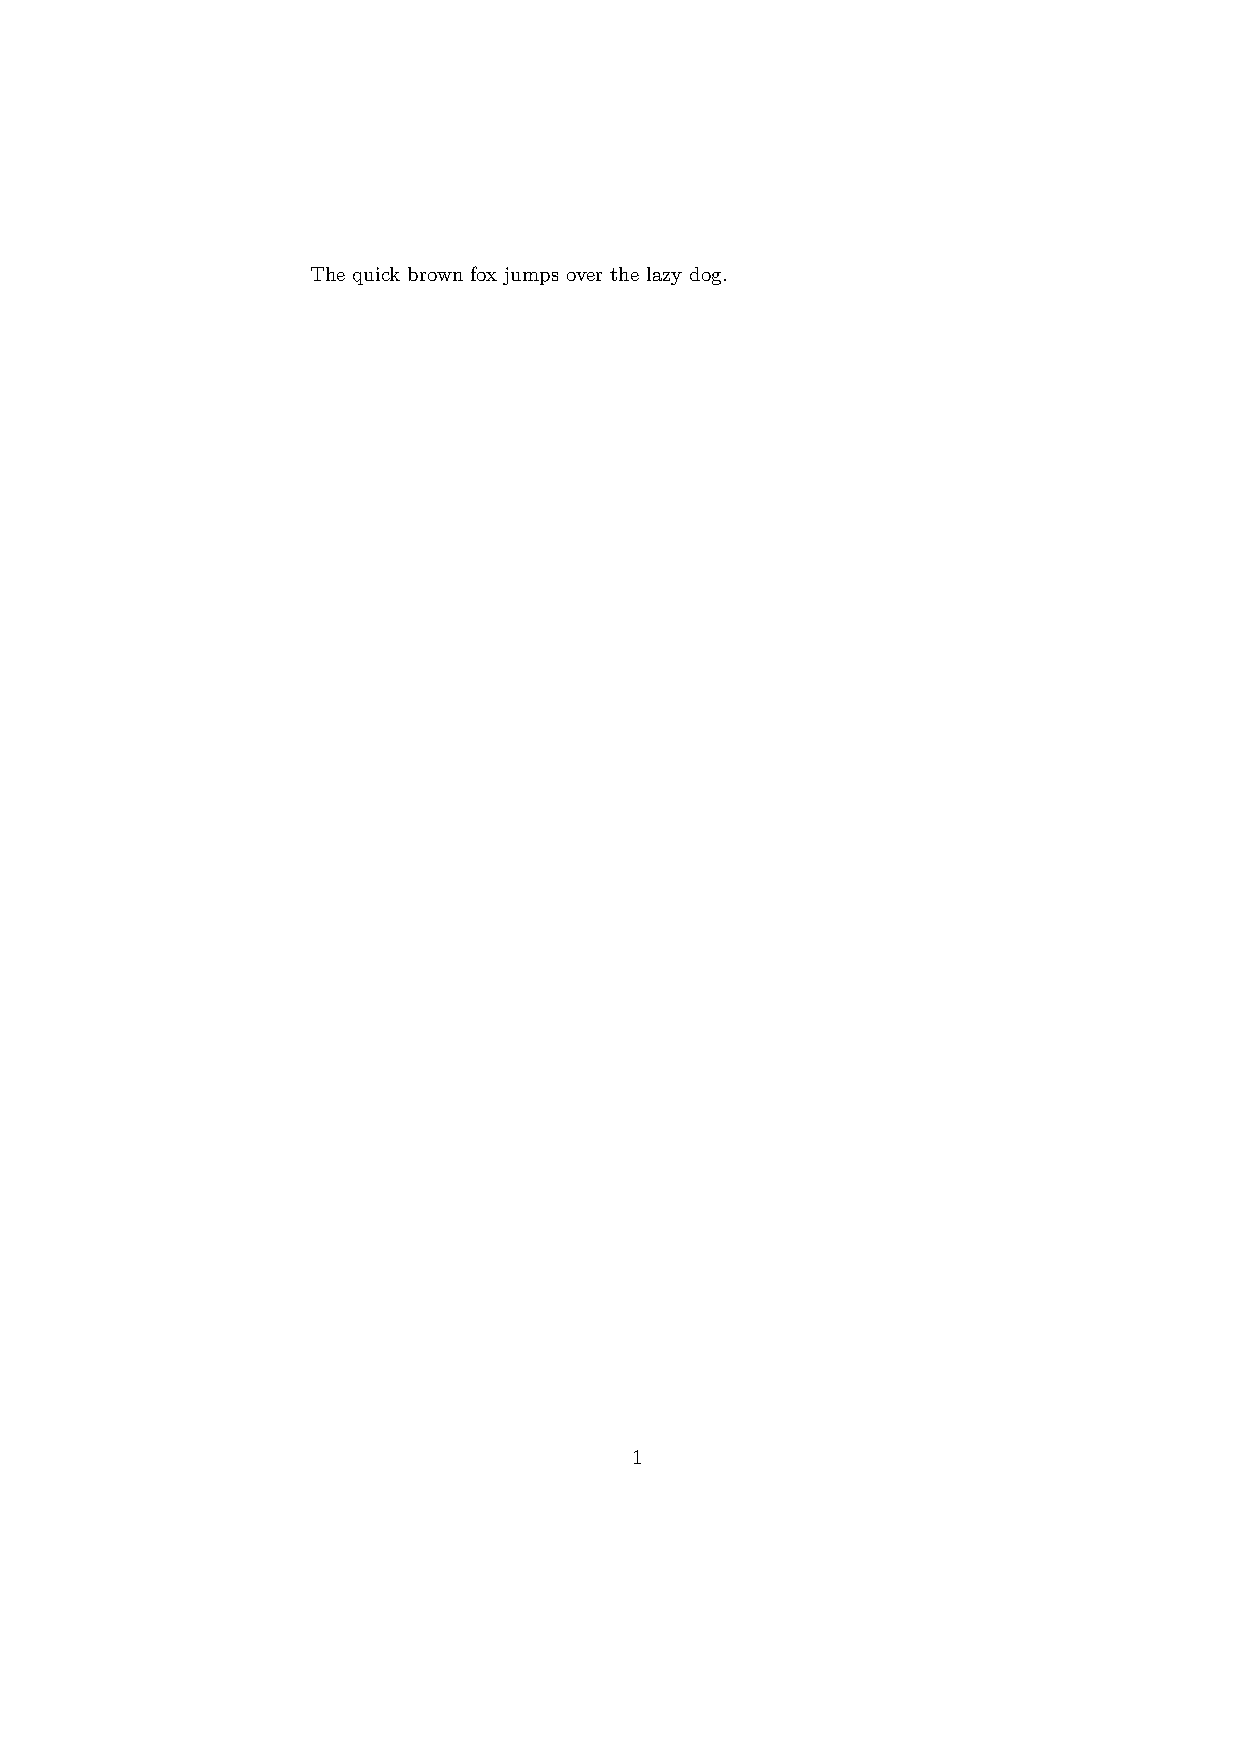
\includegraphics[width = \textwidth]{lazydog.pdf}}
        \caption{第一次编译}
        \label{fig:lazyDOG}
    \end{subfigure}\quad
    \begin{subfigure}[t]{0.4\textwidth} \centering
        \boxed{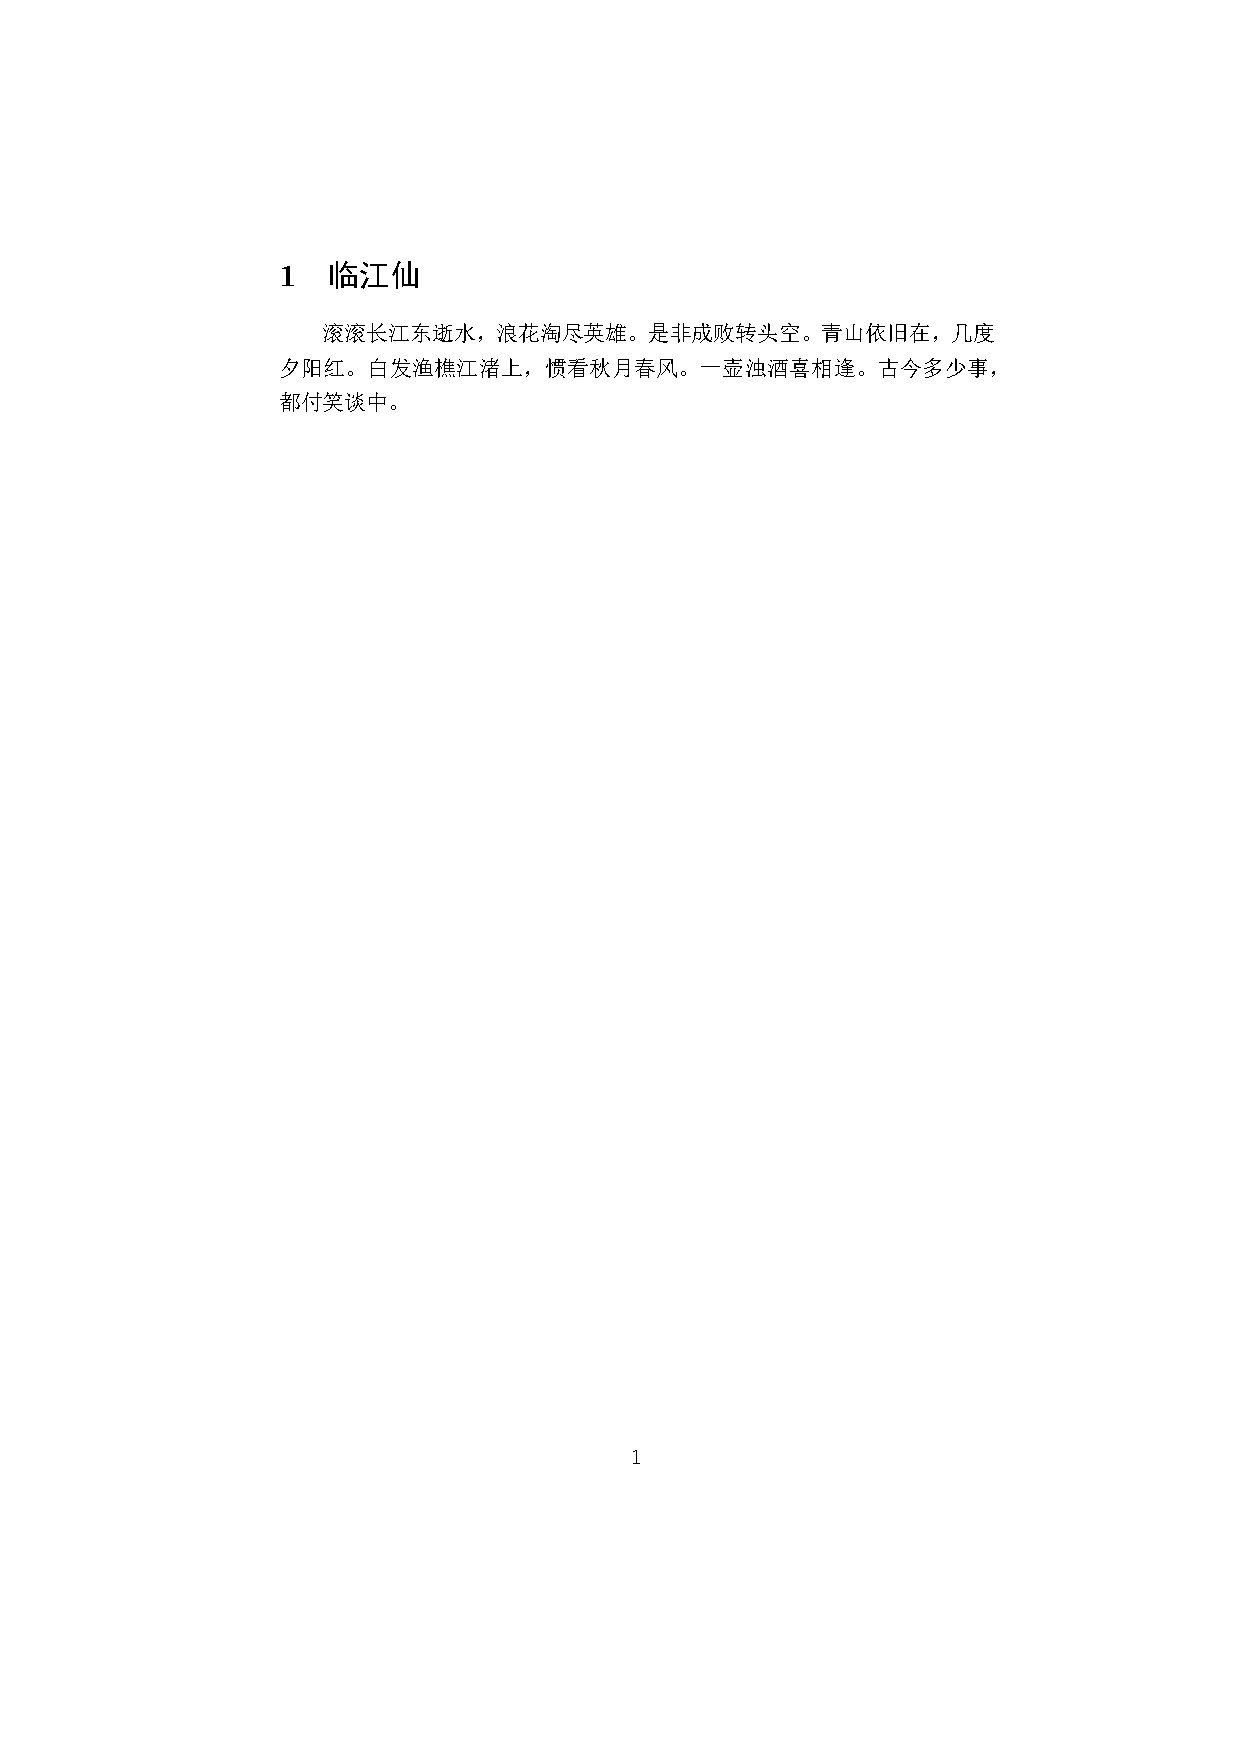
\includegraphics[width = \textwidth]{ggcjdss.pdf}}
        \caption{一个带中文的例子}
        \label{fig:滚滚长江东逝水}
    \end{subfigure}
\end{figure}

接下来写些带其他文字的例子 \autoref{fig:滚滚长江东逝水} :


\begin{lstlisting}
    \documentclass{article}
    \usepackage{ctex}
    \begin{document}
    \section{临江仙}
        滚滚长江东逝水,浪花淘尽英雄。是非成败转头空。
        青山依旧在,几度夕阳红。

        白发渔樵江渚上,惯看秋月春风。一壶浊酒喜相逢。
        古今多少事,都付笑谈中。    
    \end{document}
\end{lstlisting}


“我来解释一下这里面的命令……

\begin{itemize}
    \item \verb"\documentclass{article}" 指的是使用 \verb"article" 文档类,这意味着还有其他的文档类,比如说 \verb"book"、\verb"ctexart" 这些。
    \item \verb"\usepackage{ctex}" 是在这里引用了一个叫做 \verb"ctex" 的宏包,这个宏包正是用来处理 CJK 字符的。
    \item \verb"\begin{document}" 和 \verb"\end{document}" 之间就是咱们的正文区了,在此之前就是引言区(主要来作一些全局设置的)。
\end{itemize}

不过值得注意的是,代码的换行并不会引起 PDF 内内容的分段,至少需要连续换两行才行。”

“这看起来倒像是合乎常理的……毕竟代码不能一行写太长嘛……”

“其实倒也不是这样,因为 \LaTeX 里面的换行其实有点像空格……在某些层面影响很大的。”莲子纠正道,“我给你看个好康的例子。”


\begin{lstlisting}
    \documentclass{article}
    \usepackage{ctex}
    \begin{document}
        \colorbox{red}{
            \color{white} 
            A spanning list in a vector space may not be a basis because it is not linearly independent.
        }
    \end{document}
\end{lstlisting}

\begin{center}\footnotesize
    \colorbox{red}{
        \color{white}
        A spanning list in a vector space may not be a basis because it is not linearly independent.
    }
\end{center}

“看起来好像没啥,实际上——A 前面是有一个空格的,这个空格实际上是来自于代码换行。”

“哦哦!所以我是不能随便换行的对吧,那这样太离奇了吧?写代码不能随便换行??”

“呃……其实有方法可以规避的……我们一般会在折行处加一个 \verb"%" 符号,这样子就可以注释掉后面的换行(空格)了。”


\begin{lstlisting}
    \colorbox{red}{%
        \color{white}%
        A spanning list in a vector space may not be a basis because it is not linearly independent.%
    }
\end{lstlisting}

\begin{center}\footnotesize
    \colorbox{red}{%
        \color{white}%
        A spanning list in a vector space may not be a basis because it is not linearly independent.%
    }
\end{center}

“呒呒呒,原来注释还有这种用法。”堇子挠了挠头,“我还是第一次见。”

“以后有得你见的,有关 \LaTeX,有趣的事情不少。这种注释也只用在你想写一些正经代码的时候。”

\subsection{用 \LaTeX 组织你的文档——最初的例子}

“行了,说了那么多废话,我们来看看一个带数学公式的例子。”

“哦这么说差点忘了,之前一直在听你说故事什么的,原本自己想干什么都忘了。”

“公式嘛……其实与正文不一样,因此要提供一个‘数学环境’这样的东西。”


\begin{lstlisting}
    \documentclass{article}
    \begin{document}
        as we know:
        \[
            \sum_{n=0}^\infty \frac{1}{n!} = \exp (1)
        .\]
        and $\sin \left( \frac{\pi}{2} \right) = 1 $.
    \end{document}
\end{lstlisting}

得到 \autoref{fig:firstmath}。

\begin{figure}[th]
    \centering
    \boxed{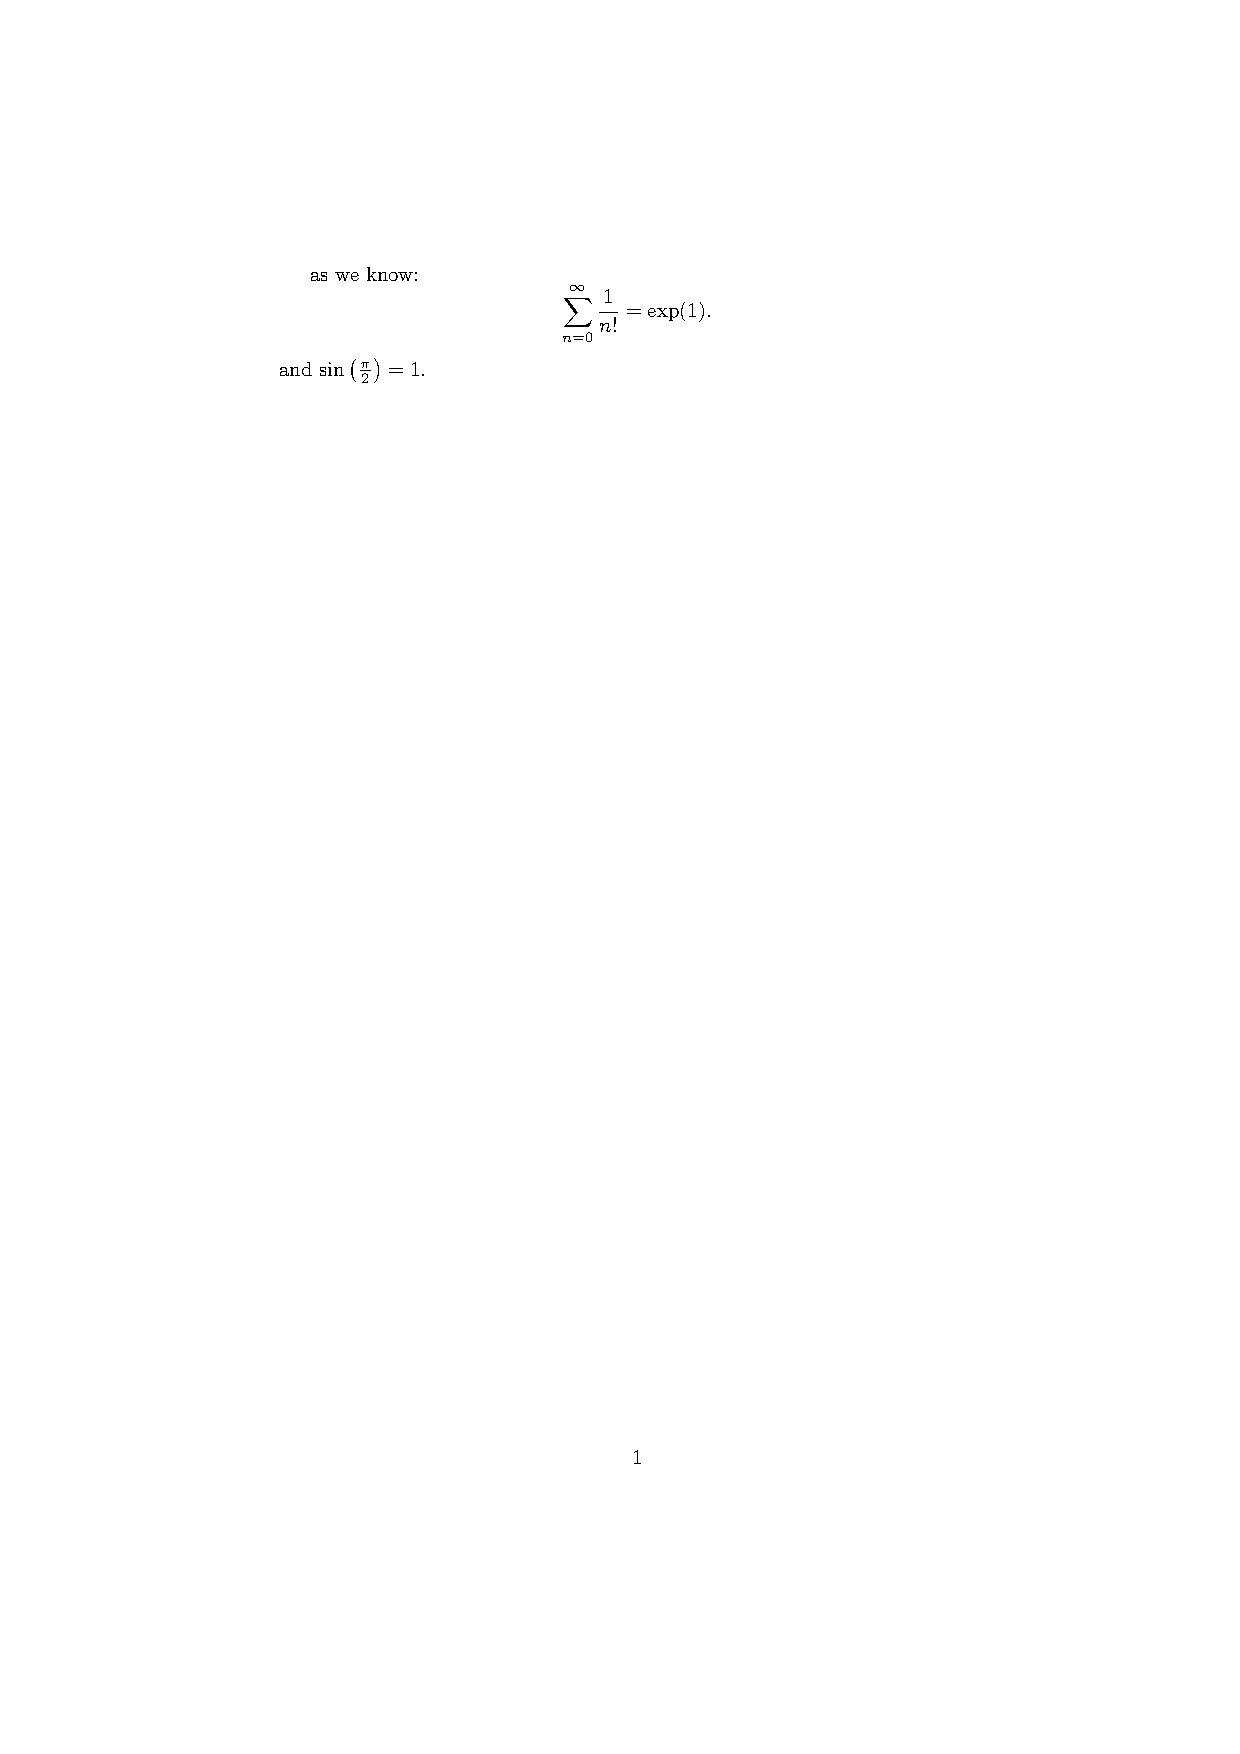
\includegraphics[width = 0.4 \textwidth]{first math ex.pdf}}
    \caption{一个带了数学环境的例子}
    \label{fig:firstmath}
\end{figure}


其中我们会认为:
\begin{itemize}
    \item \verb"\[...\]" 之间是\textbf{行间公式}环境,我们可以称为``displaystyle math''。
    \item 与之对应的,\verb"$...$" 是行内数学公式环境,可以称为``textstyle math''。
\end{itemize}

当然以上两种也可以用 \verb"$$...$$" 和 \verb"\(...\)" 来代替,虽然我不推荐\footnote{\texttt{\char"005C[...\char"005C]} 比 \texttt{\$\$...\$\$} 多了一层检查用于 \texttt{\char"005C @badmath} 报错,且还支持一些选项(比如说公式左对齐的 \texttt{fleqn} 选项、 \Verb{\tag} 命令等)而 \texttt{\char"005C(...\char"005C)} 则不是 Robust 的命令,具体见 \textcite[The \LaTeXe{} Sources]{braams2003latex2varepsilon} \link{https://www.ctan.org/pkg/source2e}。}就是了。在例子中可以很清楚对照到“上标”是 \verb"^{...}",下标是 \verb"_{...}" ,当只有一个字符的时候可以省略掉大括号。 至于像其他乱七八糟的数学符号命令现在在这里全部说明也不适合——具体可以参考——呃算了等到一会我回去的时候给你些链接。”

“链接?不会又是什么全英文地狱电子文档吧?”堇子试探性的问道。

“有些还是有翻译的。”莲子认真地说道,“总之我们继续。”

“在除去数学公式这一巨大的板块后, \LaTeX 当然可以参与普通的排版,在 \verb"article" 类中有很多章节层级,按以下顺序排列:

\begin{center}
    \begin{tblr}{cll}
        \hline
        层次 & 命令                              & 说明                                \\\hline
        $-1$ & \ttfamily\char"005C part          &                                     \\
        $0$  & \ttfamily\char"005C chapter       & \texttt{article} 类中并没有这个章节 \\
        $1$  & \ttfamily\char"005C section       &                                     \\
        $2$  & \ttfamily\char"005C subsection    &                                     \\
        $3$  & \ttfamily\char"005C subsubsection & 默认不编号、不编目录                \\
        $4$  & \ttfamily\char"005C paragraph     & 同上                                \\
        $5$  & \ttfamily\char"005C subparagraph  & 同上                                \\\hline
    \end{tblr}
\end{center}

在此机制之上我们就可以组织我们文档的层级了。”


\begin{lstlisting}
    \part{Algebra}
    \section{Groups}
    \subsection{Free groups}
    \paragraph{The constrution of free groups}
        We know $A$ is just a...
\end{lstlisting}



\begin{tcolorbox}[sharp corners]
    {\noindent\Large\bfseries Part\nobreakspace I
        \par\nobreak
        \noindent{\huge \bfseries Algebra%
            \par}\nobreak
        \vskip 2ex}
    {\noindent\Large\bfseries 1\kern2.3ex Groups}

    \vskip3.25ex\noindent{\normalfont\large\bfseries 1.1\kern2.25ex {Free groups}}\vskip1.3ex

    \paragraph{The constrution of free groups}
    We know $A$ is just a...
\end{tcolorbox}



“感觉不如 \verb"markdown"%\simpleicon{markdown}}
方便。”堇子吐槽道。

“请注意你的言辞,难道你要用 \verb"markdown" 写论文吗?”莲子正色道,“这玩意不保真啊。”

“可是我用 \verb"CSS" 也可以仿出这样的标题形状哇。”堇子反驳道。“ \verb"markdown"%\simpleicon{markdown}} 
写得多轻巧,这 \LaTeX 写之前我还要安装个 4 GiB 的大家伙。”

“好,你用 \verb"CSS" 写个正经的折行分页算法给我看看吧。”莲子面无表情地说道。

堇子不吱声了。



\section{\LaTeX 与数学排版}

“首先先说一点前置的东西——数学公式,如你所见,有上标、下标。因此是「二维」的,必然不可能仅仅靠字偶距\footnote{一般称为 kerning,一般字体在某些字母字面框对齐的情况下会显得比较难看: {Y}{a} 和 Ya 分别是在 Y 和 a 中间有无插入微小负间距的对比。}来微调,还要依靠上下的移动来达到比较好的效果——这显然是相当麻烦的。因此不要在数学环境里玩花。”

“草,这感觉要把这所见非所得的东西玩出所见即所得的形状出来。”

“我们应该知道一些规范,比如说正儿八经的公式就应该用正儿八经的数学环境:

“a - b 和 $a - b$,就分别是正文环境与数学环境的例子。因为在前者中 \verb"-" 是作为连字符呈现的,而后者是正儿八经的「减号」。正如前面展示的数学例子一样,我们用 \verb"$...$" 和 \verb"\[...\]" 来声明数学环境。”

\subsection{\AmS 与一些规范}

“进入数学环境之后,我们就不允许像在正文环境那样随意了,首先是一个痛点——在数学环境尽量避免使用非 ASCII\footnote{即
    American Standard Code for Information Interchange,你可以认为是美式键盘上可以直接输入的所有字符。} 代码,否则——:

“\verb"$A^ {ij} _{γ}$" 会得到$
    A^{ij} %_{γ}
$,这样子 $\gamma $ 显然没办法正常显示\footnote{除非你引入可以在数学环境进行特殊处理的包,比如 \texttt{unicode-math}.},如果要打出正常的希腊字母 $\gamma $只需打出 \verb"\gamma" 即可,其他希腊字母照常。

“草草,这也太离谱了,什么都不让用。”

“本身代码这种就最好纯用 ASCII 写啊,况且你不想想那是什么年代。另外还有一些事情是要注意的,那就是要按照正常的科技规范来正确输入,我们引入 \AmS{}Math 这个数学宏包——


\begin{lstlisting}
    % \usepackage{amsmath}
    \[
        \sum_{n=0}^{\infty} \frac{x^n}{n!} = \mathrm{e} ^ x
    .\]
\end{lstlisting}

自然就会得到:



\[
    \sum_{n=0}^{\infty} \frac{x^n}{n!} = \mathrm{e} ^ x
    .\]
“长得挺好看的这公式。”堇子立刻评论道。

“对,你看这个里面有这么一个命令 \verb"\mathrm",这玩意是将吸收的参数转化为 roman 字形,在科技文献中我们会一般要求自然对数的底 $\mathrm{e}$ 要正体,同理,面对虚数单位 $\mathrm{i}$,微分算子 $\mathrm{d}$ 也最后如此:
\[
    \int_0^{2\symup\pi } \mathrm{e} ^ {2 \mathrm{i} z } \,\mathrm{d}z = 0
    .\]
当然你不这么写也行,但这样看上去比较好看。

另外一个,一些函数的名字是可以用反斜杠加上函数名打出来的:

\begin{center}
    \begin{tabular}{cc}
        \verb"\sin z" & $\sin z$ \\
        \verb"sin z"  & $sin z$  \\
    \end{tabular}
\end{center}

“草我在一些论坛上面逛的就看到后面这种,难看死了。”

“对,而且也不合规范——这一点如果不熟悉的话还是要注意的。归根到底,其实是 \verb"\sin" 本身就是一个新的命令,展开后会得到正体的 $\sin $ 以及和后面的变量之间\textbf{带上空格}\footnote{其实不应该叫空格,叫glue更恰当。}。可以看到在上面的例子中,即使在代码里面加入空格,真正显示出来的也不会有空格。

“草这空格怎么那么麻烦……”

“先不管,我们看看这个神奇妙妙——\footnote{下面的「代码」默认在数学环境里,因此不加数学环境的声明了,此处参考 \textcite[Symbols defined by unicode-math]{WillRobertson} \link{https://mirrors.nju.edu.cn/CTAN/macros/unicodetex/latex/unicode-math/unimath-symb}。}:

\begin{table}[h]
    \centering
    \caption{一些数学字符的近似分类}
    \DefTblrTemplate{caption-tag}{default}{}
    \DefTblrTemplate{caption-sep}{default}{}
    \begin{tblr}{colspec = {X[-1]XX[-1]}, width = \textwidth}\hline
        分类                 & 代码                                                                                                                         & 预览                                                          \\\hline
        Opening symbols      & \texttt{\char"005C (, [, \char"005C\{, \char"005Clceil, \char"005Csqrt\{\}}                                                  & $(,~[,~\{,~\lceil,~\sqrt{}$                                   \\
        Closing symbols      & \texttt{\char"005C !, ), ], \char"005C\}, \char"005C rfloor}                                                                 & $!,~),~],~\},~\rfloor$                                        \\
        Fence symbols        & \texttt{\char"005C | = \char"005C vert, \char"005C Vert = \char"005C|}                                                       & $| = \vert,~\Vert~= \|$                                       \\
        Punctuation symbols  & \texttt{\char"005C , : ;}                                                                                                    & $, : ;$                                                       \\
        Over symbols         & \texttt{\char"005C overbrace\{a + b\}\^{}M}                                                                                  & $\overbrace{a + b}^M$                                         \\
        Under symbols        & \texttt{\char"005C underbrace\{h + k\}\_L}                                                                                   & $\underbrace{h + k}_L$                                        \\
        Accents              & \texttt{\char"005C bar\{x\}, \char"005C tilde\{x\}, \char"005C dot\{x\}, \char"005C ddot\{x\}, \char"005C mathcirc\{x\}}     & $\bar{x},~\tilde{x},~\dot{x},~\ddot{x},~\mathring{x}$         \\
        Math operators       & \texttt{\char"005C sin, \char"005C lim, \char"005C inf}                                                                      & $\sin,~\lim,~\inf$                                            \\
        BIG Math operators   & \texttt{\char"005C int\_0\^{}1 \char"005C sum\_0\^{}1 \char"005C displaystyle \char"005C int\_0\^{}1 \char"005C sum\_0\^{}1} & $\textstyle\int_0^1 \sum_0^1 \displaystyle \int_0^1 \sum_0^1$ \\
        Binary relations     & \texttt{\char"005C a+b, a\{+b\}, - ,\char"005C times, \char"005C div}                                                        & $a + b,~a{+b},~- ,\times,~\div$                               \\
        Ordinary symbols     & \texttt{\char"005C forall, \char"005C exists, \char"005C emptyset}                                                           & $\forall,~\exists,~\emptyset$                                 \\
        Relation symbols     & \texttt{\char"005C a<b, a\{<b\}, \char"005C to, \char"005C leftarrow, \char"005C mapsto}                                     & $a<b,~a{<b},~\to,~\leftarrow,~\mapsto$                        \\
        Alphabetical symbols & \texttt{\char"005C pi, \char"005C mathbf\{A\}, \char"005C mathcal\{X\}, \char"005C mathsf\{C\}}                              & $\pi,~\mathbf{A},~\mathcal{X},~\mathsf{C}$                    \\\hline
    \end{tblr}
\end{table}

“草这也太哈人了吧。”堇子大叫道。

“呃……实际上也只是展示出来而已,就是个分类,我们在里面可以看到一些有趣的细节……比如说 Binary relations 只有在前后两个都是其他数学符号的时候,两边才会安插一个空格——与 Relation symbols 的表现明显不一样,逗号和冒号都是正儿八经的标点符号,但逗号后面会有被动的空格,巨算符 (BIG Math operators) 在行间公式和行内公式形状不同等等,都是非常细节的东西。”

“哇,好~厉~害~哦!请问这些细节有什么用捏?”

“草……只是说无论你知晓与否,的确是有很多细节在里面的……这样可以让你对其保持敬畏。”
\subsection{字体与数学字体}

“在排版中,我们当然不会只用一种字体,而是使用各种各样形状的——见 \autoref{tab:字形们}\footnote{此处使用字体为:  宋体:Noto Serif CJK SC;黑体:Noto Sans CJK SC;楷体:方正楷体;西文衬线体:\TeX{} Gyre Pagella;西文无衬线体:Noto Sans;等宽字体:Iosevka。}。且不同的性质 \verb"shape", \verb"family", \verb"series" 可以叠加。”

“啦特可爱是什么意思?”堇子问道。

\begin{table}[h]
    \centering
    \caption{控制字形的主要三组参数}
    \begin{tblr}{l|l|l}
        \hline
        \Verb{{\mdseries ABCabc123啦特可爱}} & \Verb{\textup{ABCabc123啦特可爱}} & \mdseries ABCabc123啦特可爱 \\
        \Verb{{\bfseries ABCabc123啦特可爱}} & \Verb{\textbf{ABCabc123啦特可爱}} & \bfseries ABCabc123啦特可爱 \\
        \hline
        \Verb{{\itshape ABCabc123啦特可爱}}  & \Verb{\textit{ABCabc123啦特可爱}} & \itshape ABCabc123啦特可爱  \\
        \Verb{{\slshape ABCabc123啦特可爱}}  & \Verb{\textsl{ABCabc123啦特可爱}} & \slshape ABCabc123啦特可爱  \\
        \Verb{{\scshape ABCabc123啦特可爱}}  & \Verb{\textsc{ABCabc123啦特可爱}} & \scshape ABCabc123啦特可爱  \\
        \hline
        \Verb{{\rmfamily ABCabc123啦特可爱}} & \Verb{\textrm{ABCabc123啦特可爱}} & \rmfamily ABCabc123啦特可爱 \\
        \Verb{{\sffamily ABCabc123啦特可爱}} & \Verb{\textsf{ABCabc123啦特可爱}} & \sffamily ABCabc123啦特可爱 \\
        \Verb{{\ttfamily ABCabc123啦特可爱}} & \Verb{\texttt{ABCabc123啦特可爱}} & \ttfamily ABCabc123啦特可爱 \\
        \hline
    \end{tblr}
    \label{tab:字形们}
\end{table}


“没啥意思,你看看那个倾斜体,好像长得特别奇怪,这是为了在斜体环境与意大利作区分:

\begin{center}
    \textsl{a letter $a$} and \textit{a letter $a$}
\end{center}

“因为意大利体的字母和数学环境中的斜体字母差别相当小,我们在原本需要意大利体与数学环境混排的时候就可能会使用倾斜体。

“事实上我一点都没觉得它奇怪。”堇子说。

“这玩意应该算计算机时代才应用起来的东西\footnote{倾斜(罗马)体出现与20世纪30年代,但其作为经典意大利体的替代品而被广泛使用则是20世纪70年代的事了。\slshape ``Slanted roman type was introduced in the 1930s, but it first became widely used as an alternative to the conventional italic during the late 1970s.''\upshape 来自  \textcite[The \TeX book]{knuth1984texbook}。},以往的斜体 (Italic fonts) 倒是很具有手写的痕迹,而倾斜体差不多就是矩阵变换得来的。”

“除了在正文中的各种各样的字体风格,我们也需要在数学环境中如此表示——比如 $\mathcal{F}$ 表示 Fourier 变换、用 $\mathsf{C}$ 表示范畴 (Categories) 什么的。\autoref{tab:数学字形们}\footnote{本文使用的数学字体为 \TeX{} Gyre Pagella Math.} 是一些\textbf{特殊}的形状。”

% !
\begin{table}[h]
    \centering
    \caption{数学字形们}
    \begin{tblr}{colspec = {X[2]X[-1]X}, width = \textwidth}\hline
        命令                          & 预览                   & 备注                             \\ \hline
        \Verb{\mathbf{ABCabc123}}     & $\mathbf{ABCabc123}$   &                                  \\
        \Verb{\mathit{ABCabc123}}     & $\mathit{ABCabc123}$   &                                  \\
        \Verb{\mathsf{ABCabc123}}     & $\mathsf{ABCabc123}$   &                                  \\
        \Verb{\mathrm{ABCabc123}}     & $\mathrm{ABCabc123}$   &                                  \\
        \Verb{\boldsymbol{ABCabc123}} & $\symbfit{ABCabc123}$  &                                  \\
        \Verb{\mathfrak{ABCabc123}}   & $\mathfrak{ABCabc123}$ & 需要宏包 \AmS{}Fonts             \\
        \Verb{\mathbb{ABCabc123}}     & $\mathbb{ABC}$         & 在 \AmS{}Math 中只提供了大写字母 \\
        \Verb{\mathcal{ABCabc123}}    & $\mathcal{ABC}$        & 只提供了大写字母                 \\
        \Verb{ABCabc123}              & $ABCabc123$            &                                  \\\hline
    \end{tblr}
    \label{tab:数学字形们}
\end{table}

“大概就这样,我们只需要使用对用的命令就行——但是最好不要在 \verb"{}" 里面套上特殊的非字母字符,比如:


\begin{lstlisting}
    \documentclass{article}
    \usepackage{amsmath}
    \begin{document}
        \[  \mathcal{1} .\]
    \end{document}
\end{lstlisting}

这样反而会得到一个比较匪夷所思的结果——
\[
    \mathord\infty
    .\]

“草?这是什么乱码……是 bug 吗?”

“这其实是个非常有趣的现象\footnote{事实上,我们可以认为这些个数学符号都是由一组字符来指代的,我们可以用 \texttt{\char"005C mathchar} (\texttt{"} 指的是 16 进制的意思)来呼出对应的符号,比如说 \texttt{\char"005C mathchar"1350} 就是 $\sum$,实际上这个 \texttt{\char"005C mathchar"1350} 代表的大致含义是在第 1 类、第 3 族、位置 50 的符号,其中类 (class) 的含义我们暂且可以认为是——\texttt{\char"005C mathord, \char"005C mathop, \char"005C mathbin, \char"005C mathrel, \char"005C mathopen, \char"005C mathclose, \char"005C mathpunct},对应 Ordinary symbols, BIG Math operators, Binary relations, Relation symbols, Opening symbols, Closing symbols, Punctuation symbols, Variable family 这些(这样其实并不准确,关于 \texttt{mathcode} 这些涉及到的其实是原始的 \TeX{},而 Unicode-Math 这些分类要晚太多了),而族 (family) 可能可以切换到不同的字形:
    \[
        \mathchar"0041\mathchar"0141\mathchar"0241\mathchar"0541\mathchar"0641\mathchar"0741\mathchar"0841\mathchar"0941\mathchar"0A41
        .\]
    其实就是 \texttt{0041, 0141, 0241, 0541, 0641, 0741, 0841, 0941, 0A41} 对应的 \texttt{\char"005C mathchar}(这篇文章使用了 Unicode-Math 宏包,这家伙会改动某些 \texttt{mathcode},因此可能会有什么不太一样的地方),不难猜出将族从 0 变到 2 就可以实现大写字母到 Cal 大写字母的转变,但如果应用在数字的话:
    \[
        \texttt{\char"005C mathcal\{1\}: \char"005C mathchar"0031} \longrightarrow \texttt{\char"005C mathchar"0231: }\texttt{\char"005C mathord\char"005C infty: } \mathord\infty
        .\]
    而 \texttt{\char"005C mathchar"0231} 对应的是 $\infty$ 字形,因此不能够直接在仅仅使用 \AmS{}Math 包的情况下实现 Cal 形状的数字和小写字母。更具体的信息可以参考 \textcite[The \TeX book]{knuth1984texbook}。

    \CJKsout{其实就是没必要搞小写字母为了节省空间存其他符号了。}
},以后再和你说。不管如何,在引用 \AmS{}Math 的情况下尊重上面的 \autoref{tab:数学字形们} 大抵是没问题的。

以下是一个普通的例子:
\begin{lstlisting}
    \documentclass{article}
    \usepackage{amsmath}
    \begin{document}
        \[
        \boldsymbol{A} = q \int_0^\infty \frac{1}{\mathcal E^x}\,\mathrm{d} x \in \mathbb{R}^2  \cong \mathbb{C}
        .\]
    \end{document}
\end{lstlisting}

编译结果为:
\[
    \boldsymbol{A} = q \int_0^\infty \frac{1}{\mathcal E^x}\,\mathrm{d} x \in \mathbb{R}^2  \cong \mathbb{C}
    .\]
“当然这是没什么意义的公式。”

“那这个 \verb"\," 是什么玩意?”堇子问道。


\subsection{奇怪的微调}

“是的,你眼挺尖的:这个家伙和我们看到的命令完全不一样——她不是带字母的,事实上,这被称为控制字符 (control symbol),这玩意代表的实际上是一个「短空格」。我们之前说过,在数学环境下 \LaTeX{} 会忽略空格,如果我们要人为加入一些空格的话就得使用一些命令,这些命令大多数可以用控制字符呈现\footnote{事实上,这些控制字符大多不是最基层的命令 (primitive),比如说 \texttt{\char"005C ,} 会被定义为 \texttt{\char"005C mskip\char"005C thinmuskip}.}。”


“这种方法可以非常方便地在数学环境中加入空格,更为直接的办法是使用 \verb"\kern" 命令,注意不要使用大括号来包裹长度:
\begin{lstlisting}
    \documentclass{article}
    \usepackage{amsmath}
    \begin{document}
        \[
            a \kern 5em b
        .\]
    \end{document}
\end{lstlisting}

结果为:
\[
    a   \kern 5em b
    .\]
方便个鬼!堇子心里想道,这太愚蠢了,就在她即将吐槽的时候——

“我知道你肯定觉得这很麻烦,但事实上这玩意会更加精确。”莲子说,“各种控制字符代表的宽度可以参看 \autoref{tab:空格预览}。”

% !
\begin{table}[ht]
    \centering
    \caption{空格预览}
    \begin{tblr}{colspec = {Q[8em]Q[8em]}, rows = {font = \ttfamily}, row{1} = {font = \rmfamily}}\hline
        命令           & 预览                                              \\ \hline
        这儿什么都没有 & \makebox[0pt]{\color{red}|}\makebox[0pt]{|}       \\
        \Verb{\,}      & \makebox[0pt]{\color{red}|}\,\makebox[0pt]{|}     \\
        \Verb{\;}      & \makebox[0pt]{\color{red}|}\;\makebox[0pt]{|}     \\
        \Verb{\:}      & \makebox[0pt]{\color{red}|}\:\makebox[0pt]{|}     \\
        \Verb{\>}      & \makebox[0pt]{\color{red}|}\>\makebox[0pt]{|}     \\
        \Verb{\!}      & \makebox[0pt]{\color{red}|}\!\makebox[0pt]{|}     \\
        \Verb{\␣}      & \makebox[0pt]{\color{red}|}\ \makebox[0pt]{|}     \\
        \Verb{\quad}   & \makebox[0pt]{\color{red}|}\quad\makebox[0pt]{|}  \\
        \Verb{\qquad}  & \makebox[0pt]{\color{red}|}\qquad\makebox[0pt]{|} \\\hline
    \end{tblr}
    \label{tab:空格预览}
\end{table}

可惜的是,这玩意竖直上的长度并没有那么容易微调,我们可以使用 \verb"\raisebox" 实现\footnote{\LaTeX 的定义并非如此,实际上要复杂得多,具体见  \textcite[The \LaTeXe{} Sources]{braams2003latex2varepsilon} \link{https://www.ctan.org/pkg/source2e}。}:


\begin{lstlisting}
    L\kern-.36em\raisebox{.38ex}{\textsc{a}}\kern -.16em T\kern -.1667em\raisebox{-.5ex}{E}\kern -.125em X
\end{lstlisting}



\begin{center}
    L\kern-.36em\raisebox{.38ex}{\textsc{a}}\kern-.16emT\kern -.1667em\raisebox{-.5ex}{E}\kern -.125em X
\end{center}


“我们之前看到的错落有致的 \LaTeX{} 图案就可以这样仿制出来。”

“这种在 Word 这些里面也并不是那么方便……”堇子若有所思地说。

“但是我觉得这玩意没个鬼用——还是所见即所得好。”她立马改口。

“虽然是,但是 \LaTeX 和所见即所得的其他工具本身的设计思路就不一样的,反正排公式这边我还是一如既往选择 \LaTeX,嗐不过这也得看你的 BOSS 要求,”宇佐见莲子解释道,“反正 BOSS 说什么你就用什么,这也是没办法的事情啦。”

\section{参考与学习资料}

“啊时间差不多咯……我也差不多该回去了。”在偶然看了下手表之后,宇佐见莲子这样说道。“那这样,我跟你说下遇到困难应该在哪里找答案。”

“我之前说过:‘有很多面向 \LaTeX 开发的宏包可以解决各式各样的问题’。这些作者们开发的宏包实现当然不一样,因此这些问题本质上是无极限的——你又不可能不使用宏包对吧?所以我们一般只需要掌握最基础的宏包的最基础的用法就行。至于其他乱七八糟的什么宏包,我们可以在参考文献中找到——先看看这个神奇妙妙工具。”

“打开你的命令行\footnote{如果你是 Windows 用户,可以使用 \texttt{Win + R} 键打开运行窗口,输入 \texttt{cmd} 打开控制台。},输入 \verb"texdoc lshort" 然后回车。此时一般会打开个 PDF 文件 \textcite[LShort]{oetiker2003not}
——虽然是英文的地狱,但这玩意流传甚广因此由各种各样的翻译:

\begin{itemize}
    \item  \verb"texdoc lshort-zh-cn" 是打开简体中文的翻译版。
    \item  \verb"texdoc jshort" 是打开日文的翻译版。
\end{itemize}

“这就是一本很好的入门手册了,另外,也可以参考刘海洋的 \textcite[\LaTeX 入门]{刘海洋2013latex},这本比 \verb"lshort" 要厚不少,虽然内容有些过时了,但也值得一读,哦还有 \textcite[\LaTeX{} Reference Sheet for a thesis with KOMA-Script]{RSTL23KS}, \textcite[现代 \LaTeX 入门讲座]{stonezeng},这玩意可以当成奇怪的零食干货来吃。”

“太多了叭!”堇子不耐烦地说道,“这——这本几百页我看这本还不如去看代数!”

“呃……这只是参考书,你平时会去背字典吗?”莲子反问道。

“这性质不一样的吧?”

“不管莉,反正最后就这样,这书写的也是比较容易上手的,当成小入门看完全没问题——你要是有兴趣也可以去啃些其他的作品,比如说 \textcite[The \LaTeX{} Companion. Second Edition]{mittelbach2004latex}, 或者 \textcite[The \TeX book]{knuth1984texbook}。”

“这两本估计是大大怪吧?”堇子说。

“差不多,反正我这里就说一下而已。”

“另外是我自己用过的一些宏包的推荐——见 \autoref{table:一些数学宏包们} 如果不清楚具体用法的话可以 \verb"texdoc" 再加上具体的宏包名查询宏包文档:

\begin{table}[ht]
    \begin{tblr}{colspec = {X[-1]X}, width = \textwidth}\hline
        宏包名                                                               & 极其简要的备注                                                                                 \\\hline
        \ttfamily \href{https://www.ctan.org/pkg/ctex}{ctex}                 & 当下中文最佳解决方案之一                                                                       \\
        \ttfamily \href{https://www.ctan.org/pkg/amsmath}{amsmath}           & 数学相关必备宏包之一                                                                           \\
        \ttfamily \href{https://www.ctan.org/pkg/graphicx}{graphicx}         & 图像的插入与处理                                                                               \\
        \ttfamily \href{https://www.ctan.org/pkg/unicode-math}{unicode-math} & 使用 Unicode 数学字体,并且允许在数学环境中使用 Unicode 字符,是相当“现代”的数学字体解决方案   \\
        \ttfamily \href{https://www.ctan.org/pkg/mathtools}{mathtools}       & 一个提供了相当多数学公式拓展的宏包,提供了一些有用的符号                                       \\
                                                                             & (比如说长等号什么的)                                                                         \\
        \ttfamily \href{https://www.ctan.org/pkg/tikz}{tikz}                 & 著名绘图宏包,由 Till Tantau 研发,有很多拓展库                                                \\
        \ttfamily \href{https://www.ctan.org/pkg/pgfplots}{pgfplots}         & Ti\textit{k}Z 拓展库之一,可以绘制函数图像、参数方程、三维图像等                               \\
        \ttfamily \href{https://www.ctan.org/pkg/tcolorbox}{tcolorbox}       & 可以排出各种各样的神奇妙妙彩色盒子                                                             \\
        \ttfamily \href{https://www.ctan.org/pkg/tabularray}{tabularray}     & 一个比较新的但是非常厉害的表格宏包                                                             \\
        \ttfamily \href{https://www.ctan.org/pkg/fancyhdr}{fancyhdr}         & 可以方便修改页眉页脚的格式                                                                     \\
        \ttfamily \href{https://www.ctan.org/pkg/enumitem}{enumitem}         & \LaTeX 里面有两种环境叫做 \texttt{itemize} 和 \texttt{enumerate},该宏包可以比较方便更改其样式 \\
        \ttfamily \href{https://www.ctan.org/pkg/hyperref}{hyperref}         & 处理 PDF 超链接相关的问题                                                                      \\
        \ttfamily \href{https://www.ctan.org/pkg/fontspec}{fontspec}         & 一个比较现代的字体设置的宏包                                                                   \\
        \ttfamily \href{https://www.ctan.org/pkg/titlesec}{titlesec}         & 修改章节标题格式                                                                               \\\hline
    \end{tblr}
    \caption{一些数学宏包们}
    \label{table:一些数学宏包们}
\end{table}

“太多了!记不住的这玩意——而且你这形容也太抽象了……”

“呃如果想看看这玩意的用处就去看文档咯——比如那个 \verb"tcolorbox" 就很有意思。” 宇佐见莲子回答说,“反正我在这说也没啥用,你看了就知道了。如果遇到问题也可以到网上咨询:\link{https://tex.stackexchange.com}。”

言下之意就是不要打扰别人(您)嘛,堇子想道,不过这话当然不能说出来。

\

宇佐见莲子离开后。堇子作为“世界上最强种族的代表”,开始鼓捣那几十年前的老东西。

宇佐见莲子说得没错,这玩意确实排公式方便,也十分美观。但作为古老的引擎,\TeX / \LaTeX 的活力远不如现在的其他排版 / 字处理软件——\href{https://www.microsoft.com/en-us/microsoft-365/word}{Microsoft Word}、\href{https://www.adobe.com/products/indesign.html}{Adobe In Design} 等等那么充沛,这或许是 \LaTeX 所见非所得的特性和陡峭的学习曲线所致,但在排公式、科技类论文 \LaTeX 的确无出其右者,对排版细节的把握 \TeX 也是达到了相当高的水准。

是时候需要新工具了,宇佐见堇子想,整个社区都在等待着那一天。

\chapter[数分/高代在学什么?]{数分/高代在学什么?}\label{cp:数分/高代在学什么?}

\addauthor{食人妖怪}

\begin{center}
    \itshapeCJK\normalsize 食人妖怪
\end{center}


数学分析和高等代数,是每一位数学专业的新生一上来就要面对的两门课程。在这两门课程里,一切都要以严格的数学语言表达,但这些冷酷的字句后面,往往有着简单直接的想法作为直接支撑。

遗憾的是,由于教学顺序上的不合理和教材叙述的不足,这些简单直接的想法很多时候被隐藏了。这就造成了新生学习上的困难:用意义不明的符号作着莫名其妙的计算,为不知所谓的结论给出胡言乱语的证明……

通过这篇文章,我们希望尽可能简单地介绍这些课程内容背后的想法动机。我们不会给出严肃的证明,但偶尔会勾勒其想法。尽管阅读本文不能替代正经的课程学习,但或许能把你暂时变成一个“云玩家”,使你能够了解这些东西有多么好玩。
\section{数学分析}

作为一篇介绍性质的文章,我们在此仅介绍一元微积分学中的一些想法直观。多元微积分学的很多内容,都可以和一元微积分学比照学习。受限于篇幅,我们不可能面面俱到地提及全体概念,对课程的学习和思考仍是不可少的。
\subsection{实数定义,极限与连续}

我们早已接触并频繁使用实数,但实数是什么?大部分人第一次接触到的定义是“实数是有限小数和无限小数”。可是,我们只知道有限个数的加法,凭什么无穷多个数码能定义出一个无限小数呢?尽管我们能进行一些想象,但可能很难用严格的数学语言描述“无限小数”是什么。

在数学里,一切都要有严格、精确的定义。因此,
我们的第一个任务,就是合理地定义实数。

假设你已经熟知了整数的性质。通过考虑“两个数相除(分母非$0$)”,我们可以得到有理数。在有理数上,我们有四则运算,还有一个大小关系。

通过这个大小关系,我们可以暂时抛开严谨性,进行一些直观的想象。可以想象全体有理数“排列在一条直线上”。尽管有理数是“稠密”的——直线上每一小段“开区间”内都含有有理数,但是有理数之间还是有一些“间隙”,比如这个经典的例子:“长为$1$的正方形的对角线长”。

\begin{center}
    \begin{tikzpicture}[scale = 3]
        \draw[->] (-1.2, 0) -- (2.2, 0);
        \foreach \x in {1,...,10}
            {
                \filldraw (1/\x, 0) circle(0.01);
            }
        \filldraw[fill = white] (1.41421, 0) circle(0.01);
        \filldraw (2/3, 0) circle(0.01);
        \filldraw (2, 0) circle(0.01);
        \filldraw (-1, 0) circle(0.01);
        \coordinate[label = below:{\footnotesize\(\sqrt{2}\)}]() at (1.41421, 0);
        \coordinate[label = below:{\footnotesize\(2\)}]() at (2, 0);
        \coordinate[label = below:{\footnotesize\(1\)}]() at (1, 0);
        \coordinate[label = below:{\footnotesize\(\frac{1}{4}\)}]() at (0.25, 0);
        \coordinate[label = above:{\footnotesize\(\frac{1}{3}\)}]() at (1/3, 0);
        \coordinate[label = above:{\footnotesize\(\frac{2}{3}\)}]() at (2/3, 0);
        \coordinate[label = above:{\footnotesize\(\frac{1}{2}\)}]() at (0.5, 0);
        \coordinate[label = below:{\footnotesize\(0\)}]() at (0, 0);
        \coordinate[label = below:{\footnotesize\(-1\)}]() at (-1, 0);
        \coordinate[label = above:{\footnotesize\(\cdots \)}]() at (1/6, 0);
    \end{tikzpicture}
\end{center}


怎么利用有理数找到并精准地描述这些“坑”呢?Dedekind 的想法是利用“分划”:将有理数集划分为两个集合$A,B$,使得“下集合”$A$中的任一数比“上集合”$B$中全体数都小。此时我们称$(A,B)$定义了一个实数,也就是“夹在$A$和$B$中间”的那个实数。为了避免不同的分划定义同一个实数,我们进一步要求$B$中没有最小数。这样,实数集就可定义为满足上述条件的有理数划分$(A,B)$构成的集合。

有了实数集之后,可以定义我们想要的大小关系和运算:大小关系可以用分划中下集合的包含关系定义,两个元素$(A,B)$,~$(A',B')$的加法则可定义为$(A+A',B+B')$,其中
\[S+T=\left\{ \,s+t\mid s\in S,t\in T\, \right\} ,\]
容易验证相加得到的是一个分划。乘法可以类似地定义,但要小心处理一下正负号。

这种定义实数的方式比较直观,但是没有解释什么是“无限小数”。接下来我们换一种方式定义实数。我们先来看一看之前所说的“无限小数”有怎样的特征:考虑无限小数$3.1415926\cdots$,考虑一列有限小数:
\[3.14,\quad3.141,\quad3.1415,\quad3.141592\cdots.\]
这一列数虽然一直在增加,但是可以想象这列数最后会“趋向”我们尚未定义的无限小数。这是因为这列数“摆动”的幅度在减小。数列中第一项以后的任一项和第一项的差值不超过$0.01$,第二项以后任一项和第二项的不超过$0.001$……以此类推。无论给出多么小的一个“幅度”$\varepsilon$,我们都可以找到某个$N$,使得在第$N$项后任两项的差的绝对值都不会超过这个幅度$\varepsilon$。我们将这个特征推广到一般的有理数列$\{a_n\}$,用严肃的数学语言\footnote{“$\exists$”相当于“存在”,“$\forall$”相当于“对于任意的”。}描述如下:
\[\forall \varepsilon>0,\,\exists N,\,\forall  m,n\geqslant  N,\,|\,a_m-a_n|\leqslant  \varepsilon.\]
我们将这样的数列称为Cauchy列,定义里用到的就是所谓的$\varepsilon$-$N$语言\footnote{在我们定义出实数之前,$\varepsilon$只能是有理数。但我们定义出实数之后,$\varepsilon$可以在实数中取值。}。此时我们称数列$\{a_n\}$定义了一个实数,也就是直观上$\{a_n\}$“逐渐靠近”的那个实数。

当然,两个数列可能会靠近“同一个数”。比如常值数列$\{0\}$和数列$\{ 1/n\}$。直观上,这两个数列都是“逐渐靠近$0$”的。因为给定一个幅度$\varepsilon$,都存在一个$N$,使得在$N$项之后,每一项与$0$的差的绝对值不会超过$\varepsilon$。我们可以继续使用$\varepsilon\text{-}N$来定义这件事:称数列$\{a_n\}$收敛至$a$或$a$是$a_n$的极限,如果
\[\forall \varepsilon>0,\,\exists N,\,\forall n\geqslant  N,\,|\;\!a_n-a|\leqslant  \varepsilon.\]
我们将其记为
\[\lim a_n=a.\]
称两个Cauchy列$\{a_n\}$,~$\{b_n\}$定义同一个实数,
当且仅当$\{a_n-b_n\}$收敛至$0$。我们也可以在如此定义的实数集合上定义四则运算和大小关系,篇幅所限不再赘述。

刚刚对数列收敛和极限的定义,也可以对实数数列进行。在实数上,收敛于某个实数的数列和Cauchy列是完全等价的。可以证明,极限可以和基本的四则运算交换:
\[
    \lim(a_n+b_n)=\lim a_n+\lim b_n,\quad\lim(a_n\cdot b_n)=\lim a_n\cdot \lim b_n,
\]
\[\lim b_n\neq 0,\quad\lim \frac {a_n}{b_n}=\frac{\lim a_n}{\lim b_n}.\]
只要等式右侧的所有极限存在。

数列$\{a_n\}$的极限可以看作$n$走向“无穷大”时,对数列状态的描述。有时我们会使用记号$+\infty$和$-\infty$指代正的“无穷大”和负的“无穷大”。需要注意的是,这两者并不在我们定义的实数之内,我们没有赋予其任何意义。因此,我们一般不会让$\pm\infty$参加可能引起歧义的运算,但也可以定义数列$\{a_n\}$数列“趋于”$+\infty$(或相应地,$-\infty$):若
\[\forall  M>0,\,\exists N,\,\forall n\geqslant  N,\,a_n\geqslant  M,\]
则称$\{a_n\}$趋于$+\infty$。

通过数列极限,我们可以定义怎样对无穷多个数“求和”:对数列$\{a_n\}$如果部分和的序列$A_n=a_1+\cdots +a_n$收敛于$A$,则称$A$是数列$\{a_n\}$的和。此时我们也说,级数
$\sum_{n=1}^{+\infty}\,a_n$
收敛。

一般来说,无穷求和不能保证项之间可以随意交换,比如
$\sum_{n=1}^{+\infty}\,\dfrac{(-1)^{n-1}}{n}$
是收敛的,但如果将求和中的项重新排序,新得到的级数和可以收敛到任何一个实数,也可能根本不收敛。其原因在于级数的“总振幅”
\[\sum_{n=1}^{+\infty}\,\left|\dfrac{(-1)^{n-1}}{n}\right|=\sum_{n=1}^{+\infty}\,\dfrac{1}{n}.\]
是趋于正无穷的\footnote{这个结论称为Riemann重排定理。}。如果
$\sum_{n=1}^{+\infty}\,|a_n|$
是收敛的,我们称级数$\sum_{n=1}^{+\infty}\,a_n$
绝对收敛。此时级数的项可以随意交换顺序。

数列可以看作定义在正整数上的“函数”。因此除了考虑数列的极限,我们还可以考虑一般的函数的极限。函数极限的种类要更丰富:不仅有自变量趋于正无穷/负无穷时的极限,还有趋于某个实数$x_0$时的极限。前两者和数列的情形大同小异,值得注意的是后一种情形:设有实数$a$和函数$f$,如果$f$在$x_0$周围——或者说,$x_0$的某个“邻域”$(x_0-h,x_0+h)$上有定义,且
\[\forall \varepsilon>0,\,\exists \delta>0,\,\forall x,\,0<|x-x_0|\leqslant  \delta,\,\bigl|\,f(x)-a\bigr|\leqslant  \varepsilon,\]
则称$a$是函数$f$在$x$趋于$x_0$处的极限,记为
\[\lim_{x\to x_0}f(x)=a.\]

在这个定义里面,如果将对$x$的要求从$|x-x_0|\leqslant  \delta$改成$x_0<x\leqslant  x_0+\delta$,即只在$x_0$的右侧变动,则称$a$是$f$在$x_0$的右极限。完全类似地,也可定义左极限。我们分别使用记号
\[\lim_{x\to x_0^+},\quad \lim_{x\to x_0^-}.\]

细看函数极限的定义,可以发现$x$不能取$x_0$。这是因为我们希望研究函数在$x_0$周围的性状,但函数本身在$x_0$可能有定义,所以需要排除掉函数在$x_0$的取值对周围性状的影响。比如下面的函数:
\[f(x)=
    \begin{dcases}
        0, & x\neq 0; \\
        1, & x=0.
    \end{dcases}
\]
$f$在$0$周围的取值都是$0$,但是$f(0)=1$。按照定义,此时函数在$0$处的极限是$0$而非$1$。

\begin{center}
    \begin{tikzpicture}[scale = 1.5]
        \draw[->] (-3.2, 0) -- (3.2, 0);
        \draw[thick] (-3.2, 0) -- (3.2, 0);
        \draw[->] (0, -1) -- (0, 2);
        \filldraw[fill = white, thick] (0, 0) circle(0.03);
        \filldraw[thick] (0, 1) circle(0.03);
        \coordinate[label = -135:{\(0\)}]() at (0, 0);
        \node[]() at (0.5, 0.5){\footnotesize\(f(0)=1\)};
    \end{tikzpicture}
\end{center}

直观上看,这种现象的出现是由于$f$的图像在$0$处“断掉了”。我们可以以此定义函数的“连续性”:
设函数$f$在$x_0$的某个邻域$(x_0-h,x_0+h)$上有定义,同时
\[\lim_{x\to x_0}f(x)=f(x_0),\]
则称$f$在$x_0$连续;

如果$f$在某个开区间$I$(特别地,$I$可以取成全体实数)上有定义且在$I$中每一点连续,则称$f$在$I$上连续;

至于闭区间,我们只要在端点处用相应的单侧极限代替极限,就可以得到闭区间上连续函数的定义。

“连续”是一个基础而重要的概念,值得反复探讨。首先,根据连续性的定义,每一个局部的“连续”可以决定整体的连续。其次,我们可以用“小片”上的连续函数“粘”出“大片”上的连续函数:设开区间$I$可以分解为一些小开区间$I_j$之并。如果对每个$I_j$分配一个$I_j$上的连续函数$f_j$,使得在任两个区间$I_j$,~$I_{j'}$重叠的部分,$f_j$,~$f_{j'}$的取值也相同。那么我们可以得到一个$I$上的连续函数$f$。反过来,$I$上的连续函数$f$也可以将定义域限制在每个开区间$I_j$上,得到一族连续函数$f_j$。这种限制与粘合的构造是许多数学概念的源头。

从直观上看,连续就是“不断”。如果一个画在$xOy$平面上的函数一部分在$x$轴以上,一部分在$x$轴以下,那么一定要和$x$轴相交——这就是连续函数的介值定理,可以用来证明某些方程的解存在。

我们可以回头看一看我们是如何定义出连续的,这主要依赖于我们对“距离”的刻画——绝对值函数$|x-y|$。在某些场合,我们处理的“函数”不再是定义在实数上的,如果此时我们仍能定义一个满足一定条件的“距离”,我们依然可以讨论连续性。

但即使是这个条件,有时也显得过于苛刻。我们可以干脆将“距离”也抛弃掉,转而使用“邻域”来刻画连续性:设$f:X\to Y$,设$x_0\in X$,如果对$f(x_0)$不论多么“小”的邻域$V$,都可以找到$x_0$的一个“小”邻域$U$,使得$f$将$U$整个映到$V$内部,那么就称$f$在$x_0$连续。我们只需要给出“邻域”的足够精当的描述,这正是点集拓扑的内容。数学分析里的不少内容,都能看出点集拓扑学的影子。如果你学有余力,学一些点集拓扑的帮助是很大的。
\subsection{导数和积分}

我们在高中的时候介绍过导数的概念,当时我们使用的是“切线”的几何直观。现在,我们以“逼近”的角度来重新认识导数。

贯穿分析学的一个想法是“以好对象逼近坏对象”。因此对一些性质较好的函数,我们可以尝试在某一点$x_0$附近以“线性函数”进行逼近。这个一次函数的斜率就是我们说的导数$f'(x_0)$,其定义为
\[f'(x_0)=\lim_{x\to x_0}\dfrac{f(x)-f(x_0)}{x-x_0}.\]
在$x_0$点附近,对于一个很小的增量$\Delta x$,函数值$f(x_0+\Delta x)$可以被线性函数$f(x_0)+f'(x_0)\cdot\Delta x$逼近。

对两个函数$f$,~$g$,在$x_0$附近我们将$f$,~$g$分别用相应逼近的线性函数代替,作加法、乘法\footnote{我们在得到的结果中舍去$(x-x_0)^2$项,因为它比$x-x_0$衰减地更快。}、复合,就可以看到导数之间的关联:
\[\bigl(\,f+g\bigr)'(x_0)=f'(x_0)+g'(x_0),\quad\bigl(\,fg\bigr)'(x_0)=f'(x_0)g(x_0)+f(x_0)g'(x_0),\]
\[\bigl(\,f\circ g\bigr)'(x_0)=f'(g(x_0))g'(x_0).\]

某种意义上,这是“最佳”的逼近。根据极限的四则运算,
\[\lim_{x\to x_0}\dfrac{f(x)-f(x_0)-f'(x_0)(x-x_0)}{x-x_0}=0.\]
也就是说,误差项$f(x)-f(x_0)-f'(x_0)(x-x_0)$在$x_0$附近“衰减”地比线性函数更快。我们已经不能通过调整一次项的系数,使误差在$x_0$周围减小地更快了。

为了进一步捕捉误差,我们可以使用衰减更快的项$(x-x_0)^k$,即用多项式函数来逼近$f$。当函数$f$的性质足够好时,我们有Taylor展开:

\begin{align*}
    f(x) & =  f(x_0)+\frac{f'(x_0)}{1!}(x-x_0)+\frac{f''(x_0)}{2!}(x-x_0)^2+\frac{f^{(3)}(x_0)}{3!}(x-x_0)^3 \\
         & \mathrel{\phantom{=}}+\cdots+\frac{f^{(n)}(x_0)}{n!}(x-x_0)^n+R_{n+1}.
\end{align*}


其中$f^{(n)}=\left(\, f^{(n-1)} \right)'$,~$\,f^{(1)}=f'$,$R_{n+1}$是一个比$(x-x_0)^n$衰减更快的余项。这个展式可以帮助我们计算很多奇怪的极限,但将大量的时间花费在这种计算上未必是明智之举。


积分的想法则来源于计算“面积”——尽管我们并没有定义什么是面积。按照我们朴素的想法,矩形的面积应该等于邻边相乘,同时面积应当具有某种“可加性”。于是对曲线下方图形的面积,我们可以尝试用一列矩形进行逼近。比如对定义在闭区间$[a,b]$上的函数$f$,我们可以选取矩形端点落在$x$轴上的位置分别是$a=x_0<x_1<\cdots  <x_n=b$。同时,我们选取每个矩形的“高度”:一种取法是在小段$[x_{i-1},x_{i}]$里面任意地选取一点$\xi_i$,将$f(\xi_i)$作为矩形的高。这样选取之后,计算出来小矩形的面积和\footnote{当然,$f$可以取负值。此时我们寻求的“面积”并不是直接的“面积”,而是指“带符号的面积”,即在$x$轴上方的部分和$x$轴下方部分面积的差值。}就是:
\[\sum_{i=1}^n  \,f(\xi_i)(x_i-x_{i-1}).\]

当然,上面的和式和我们真正需要的面积会有一定的“差距”,这些差距来源于矩形和曲线之间的部分。直观上看,如果我们的矩形的宽能够都选得更小,那么这些矩形和曲线就会“贴得更近”,得到的误差也会更小。

利用之前学习的经验,我们用$\varepsilon\text{-}\delta$语言来叙述这件事:如果存在实数$A$,对于任意的$\varepsilon>0$,都存在$\delta>0$,使得各个区间$[x_{i-1},x_i]$的长度均不超过$\delta$时,无论$\xi_i$如何选取,总有
\[\left|\,\sum_{i=1}^n  \,f(\xi_i)(x_i-x_{i-1})-A\,\right|\leqslant  \varepsilon.\]
那么我们称$A$是函数$f$在区间$[a,b]$上的定积分,记为
\[\int_a^{b} \,f(x)\,\mathrm{d}x.\]

定积分的存在通常需要一些具体的条件来保证,比如函数在闭区间上连续。通过定积分,我们可以为一些比较“规整”的图形定义面积,满足区域可加性并且符合我们以往的认知。

一个意外之喜是,通过积分我们可以发现求导数的“逆运算”。设$f$在全体实数上有定义且连续,固定一点$a$,我们考虑
\[F(x)=\int_{a}^x\,f(t)\,\mathrm{d}t.\]
其中$x$是$F$的变量\footnote{当$x<a$,我们定义$F(x)$为$f$在$[x,a]$上定积分的相反数,因为我们改变了方向。},而$t$是积分使用的变量。

当$x$在$x_0$处产生一个小增量$\Delta x$时,可以想象,“增加的面积”可以被宽为$\Delta x$,高为$f(x_0)$的小矩形逼近。结合我们之前有关导数“线性逼近”的介绍,可以发现此时$F'(x_0)=f(x_0)$。这样,我们就找到了一个函数$F$,使得$F'=f$。由于常函数求导为$0$,$F$加上任何一个常数都满足同样的性质\footnote{这也能说明为什么我们可以任意地选取起点$a$。}。

反过来,如果我们找到了一个函数$F$,$F'=f$,那么它和我们之前寻求的定积分相差某个常数。这是我们计算定积分的一个重要的依据,也就是著名的牛顿-莱布尼兹公式:
\[\int_a^b\,f(x)\,\mathrm{d}x=F(b)-F(a).\]
我们可以拿这个公式算出许多我们关心的面积。

按我们上面定义积分的方式,被积函数$f$是不能和连续函数相差太远的\footnote{相应的结论是黎曼-勒贝格定理。}。这给我们定义“面积”带来了一定的限制。我们可能会遇到长相千奇百怪,极不规整,相当“丑陋”的点集,这时用矩形去逼近面积是完全不可能做到的,上面做出的种种努力也都失效了。

为此,我们要回到“面积”的本质——可加性上面,小心地探讨何时可以“定义面积”,怎样用面积得到函数的“积分”,又有哪些函数可以计算积分……这就是测度论所研究的内容了。你可能会在后续的实分析课程上见到这些,并且重建一套被称为Lebesgue积分的新积分体系——但对初学者而言,最好还是从这些基础内容脚踏实地地学起。
\subsection{函数列与函数级数}
之前我们定义了数列的极限,并以此定义了数项级数的求和。完全类似地,如果我们将数列的每一项换成关于某个变量$x$的函数$f_n(x)$,就可以得到相应的函数列和函数项级数。

如果对每个$x$值,相应的数列$f_n(x)$或级数$\sum_{n=1}^{+\infty}\,f_n(x)$收敛,我们就称函数列(函数级数)逐点收敛。为了方便,我们暂且讨论函数列的收敛,函数项级数的收敛是完全类似的。

对每个$x$,记$f_n(x)$的极限为$f(x)$,这是一个新的函数。通常来说,我们取的$f_n$是熟知的、性质较好的函数,但其极限$f$是我们了解较少的对象。我们要问,能否从$f_n$的性质推知$f$的性质?如果可以,我们就可以通过对研究“好函数”$f_n$得到“坏函数”$f$的性质。

我们先从相对比较简单的连续性入手。如果$f_n$都是连续的,可以推出$f$是连续的吗?很容易发现如下的反例:取$[0,1]$上的函数$f_n(x)=x^n$,则其极限为
\[f(x)=
    \begin{dcases}
        0, & 0\leqslant  x< 1; \\
        1, & x=1.
    \end{dcases}
\]
很明显不是连续函数。

为什么$f$会在$1$附近断开?当$x\in(0,1)$逐渐靠近$1$时,$f_n(x)$虽然总是收敛于$0$的,但其收敛的“速度”会越来越慢。无论对多么大的正整数$N$,在$x=\dfrac {1}{\sqrt[N]{2}}$处,$f_N(x)$的值都是$\dfrac 12$而与$0$相距甚远。

这个现象告诉我们,对函数列而言,除了逐点的收敛性,我们还要关注“不同$x$之间”的收敛速度会不会相差太远。我们以此定义一致收敛的概念:对函数列$\{\;\!f_n\}$,若
\[\forall \varepsilon>0,\,\exists N,\,\forall n\geqslant  N,\,\bigl|\,f_n(x)-f(x)\bigr|\leqslant  \varepsilon,\,\forall x,\]
则称函数列$\{f_n\}$一致收敛至$f$.

虽然这个定义乍一看和数列极限区别不大,但其精髓在于$N$ 无关$x$的选取。我们可以比较逐点收敛的叙述:
\[\forall x,\,\forall \varepsilon>0,\,\exists N,\,\forall n\geqslant  N,\,|\,f_n(x)-f(x)|\leqslant  \varepsilon.\]
两者虽然形式上极度相似,但表达的含义是截然不同的。

在相应的函数列一致收敛\footnote{注意到,命题在更弱的条件下依然成立:相应的函数列在每一个子闭区间内一致收敛。比如在全体实数上收敛的幂级数,通常就不是一致收敛的,但在子闭区间$[-M,M]$上,我们可以用$M$进行控制。}的设定下,我们也可以通过$f_n$的导数或积分得到$f$的导数或积分。如果$f_n'$一致收敛,则
\[f'(x)=\lim f_n'(x).\]
如果$f_n$一致收敛,则
\[\int_a^b\,f(x)\,\mathrm{d}x=\lim \int_a^b\,f_n(x)\,\mathrm{d}x.\]
形式上,这些操作相当于“交换极限和导数/积分”。通常来说,这种交换次序的操作都需要某种一致性来保证。

现在,我们可以用函数列/函数项级数来研究函数。之前我们提到,性质好的函数可以用多项式逼近。为了扔掉难以捉摸的余项,我们自然希望可以“无限地”展开下去:
\[f(x)=f(x_0)+\frac{f'(x_0)}{1!}(x-x_0)+\frac{f''(x_0)}{2!}(x-x_0)^2 +\cdots+\frac{f^{(n)}(x_0)}{n!}(x-x_0)^n+\cdots\, .\]
这促使我们研究形如$\sum_{n=1}^{+\infty}\,a_nx^n$的幂级数。我们可以研究其在怎样的区域内收敛或一致收敛,是否收敛于我们想要的函数,等等。

可以证明,幂级数$\sum_{n=1}^{+\infty}\,a_nx^n$会在某个以原点为中心,半径$r$(可能为$0$或$+\infty$)的圆盘 内部绝对收敛,在外部发散,而在边界圆周上则既可能收敛,又可能发散。比如下面两个幂级数
\[\sum_{n=0}^{+\infty}x^n=\frac 1{1-x},\quad \sum_{n=0}^{+\infty}(-1)^nx^{2n}=\frac{1}{1+x^2}.\]
都仅在$|x|<1$时收敛。前者很容易理解,是由于函数在$1$附近的奇异性。但后者该作何解释?只有把关心的范围从实数扩大到复数,并对复变量的函数定义极限、导数、积分这些概念,才能得到令人满意的解释。而这一切都将会是复分析学习的内容。

\section{高等代数}
我们即将学习的代数学,并不仅仅是中学数学中的简单计算。粗略地讲,我们希望研究集合上的各种代数结构。按常见的课程划分,“线性代数”和“抽象代数”是这方面比较基础的两门课程。

虽然这两门课被安排在不同的阶段,但其内容之间是紧密关联的。而“高等代数”课程的定位通常介于这两者之间,是在线性代数的基础上加一点点抽象代数的内容。
本文主要介绍线性代数的内容,但也会体现一些抽象代数的观点。
\subsection{“结构”与线性空间}
我们高中就接触过简单的集合论。不严谨的说,集合就是一堆“元素”构成的一个整体。设有集合$A$,~$B$,如果我们对集合$A$中每一个元素$a$都按某种法则指定一个确定的$B$中元素$f(a)$,我们就得到从$A$到$B$的一个映射$f$。如果对每一个元素$a\in A$,有且仅有一个$b\in B$使得$f(a)=b$,我们称$f$是双射或一一对应。此时有逆映射$f^{-1}:B\to A$,使得$f^{-1}\bigl(\,f(a)\bigr)=a$。

虽然集合已经是相当基本的数学对象,但仅有集合是不够的。举例而言,我们所说的“自然数”实际上要比“自然数集”多出了不少信息。在一个集合里,元素之间通常是“没什么关系”的,但“自然数”并非如此。自然数之间可以进行运算和比较,比如我们熟知的加法、乘法和大小关系。正整数相加、相乘的结果不会跑出正整数集,所以加法和乘法两种运算实际上都是映射\footnote{对集合$A$,~$B$,定义Descartes积$A\times B$为其元素的有序对组成的集合:$\{(a,b)\mid a\in A,b\in B\}$。
}:$ \mathbb{N}\times\mathbb{N}\to \mathbb{N}$。而大小关系$\leq$实际上是$\mathbb{N}\times\mathbb{N}$满足某些条件的一个子集,$(x,y)$在这个子集中当且仅当$x\leqslant y$。这些额外的“信息”就可称为自然数集合上的“结构”。

现在我们考虑大一些的数集,比如有理数集$\mathbb{Q}$。由于有理数对加法和乘法封闭,加法和乘法都是$\mathbb{Q}\times\mathbb{Q}\to\mathbb{Q}$的映射,满足我们熟知的交换律、结合律以及乘法对加法的分配律。$0$和$1$分别是加法、乘法的“单位元素”,这就是说对任意$x\in\mathbb{Q}$,
\[0+x=x+0=x,\quad 1\cdot x=x\cdot 1=x. \]

每个元素$x\in\mathbb{Q}$都有加法逆元,即存在元素$-x$,使得\[-x+x=x+(-x)=0.\]每个$\neq 0$的元素$x$都有乘法逆元,即存在元素$\dfrac 1x$,使得\[x\cdot \dfrac{1}{x}=\dfrac{1}{x}\cdot x=1.\]实数集$\mathbb{R}$、复数集$\mathbb{C}$也都有完全一样的性质。我们将包含$\mathbb{Q}$且满足上述条件的$\mathbb{C}$的子集称为数域。通俗地说,数域就是对加减乘除(除数非$0$)都封闭的数集。在数域里,我们可以随意地进行四则运算而不必担心超出我们考虑的范围。

我们高中还接触过“向量”的概念。在平面$\mathbb{R}^2$上,始于原点的向量按照终点的位置和$\mathbb{R}^2$上的点一一对应。通过这个对应,我们对向量进行的一切操作可以视同对$\mathbb{R}^2$内的元素进行。我们回忆几个操作:

向量加法:对$(a,b)$,~$(c,d)\in\mathbb{R}^2$,$(a,b)+(c,d)=(a+b,c+d)$。这个加法满足交换律、结合律,且有零向量$(0,0)$作为加法的单位元素,每个向量$v$都有加法逆元$-v$。

向量数乘:对$(a,b)\in\mathbb{R}^2$和$k\in\mathbb{R}$,有$k (a,b)=(ka,kb)$。这是一个映射:$\mathbb{R}\times\mathbb{R}^2\to\mathbb{R}^2$,同样满足某种意义上的“结合律”和“分配律”:对$v$,~$v'\in \mathbb{R}^2$,$k$,~$k'\in\mathbb{R}$,我们有
\[k(v+v')=kv+kv',\quad (k+k')v=kv+k'v,\quad k(k'v)=(kk')v,\quad 1v=v.\]

我们将这个结构提炼出来,就可以得到线性空间的概念:

设$F$是一个数域,$V$是一个集合,定义了一个加法$V\times V\to V$和一个数乘$F\times V\to V$,使得上述条件均满足,就称$V$是数域$F$上的线性空间或向量空间。

需要注意的是,线性空间是架在集合上的结构。一个集合上可以赋予不同的运算,使其成为不同的线性空间。原则上,当我们谈及某个具体的线性空间时,必须明确集合上配备了什么运算。但当运算容易从上下文中看出时,我们常常略去这一点。

我们在定义中对底集合没有任何的要求,因此可以在各种各样的集合上建立起线性空间的结构。正是这种定义上的广泛性,赋予了线性代数理论强大的生命力。我们来看几个例子:

平面上的向量(视同$\mathbb{R}^2$)按我们刚刚所说,是$\mathbb{R}$线性空间。对“高维空间”$\mathbb{R}^n$中始于原点的向量(视同$\mathbb{R}^n$),也可以用类似的方式定义运算,从而为$\mathbb{R}^n$赋予了$\mathbb{R}$上线性空间结构。

记$C[a,b]$为非空区间$[a,b]$上全体实值连续函数的集合。那么函数的加法和乘以常值函数赋予了$C[a,b]$以$\mathbb{R}$上线性空间结构。

记系数在数域$F$上以$x$为变元的全体多项式的集合为$F[x]$,以通常多项式的加法和数乘作为运算,就赋予了$F[x]$一个$F$上线性空间结构。

考虑如下的齐次线性方程组:设$a_{ij}\in\mathbb{R}$,
\[
    \begin{dcases}
        a_{11}x_1+a_{12}x_2+\cdots+a_{1n}x_n=0, \\
        a_{21}x_1+a_{22}x_2+\cdots+a_{2n}x_n=0, \\
        \mathord{\cdots}\mathord{\cdots}        \\
        a_{m1}x_1+a_{m2}x_2+\cdots +a_{mn}x_n=0.
    \end{dcases}
\]
记其所有解$(x_1,\,\dots\,,x_n)$构成的集合为$X\subset \mathbb{R}^n$,则$X$中元素对$\mathbb{R}^n$上的加法和数乘封闭,因而有了$\mathbb{R}$上线性空间结构。

$X$本身是$\mathbb{R}^n$的子集,$X$上的线性空间结构又完全继承自$\mathbb{R}^n$。此时我们称$X$是$\mathbb{R}^n$的子空间。

上面几个例子中的对象出现在数学的不同领域中。我们再一次看到线性代数理论的重要性。

\subsection{基、线性映射与矩阵}
我们继续关注平面向量这个我们比较熟悉的例子。高中时我们曾经学过平面向量基本定理:如果$u,v$是不共线的向量,那么平面上的每一个向量都可唯一地表成$au+bv$的形式。对空间向量也有类似的结果,只是此时是三个不共面的向量。

\begin{center}
    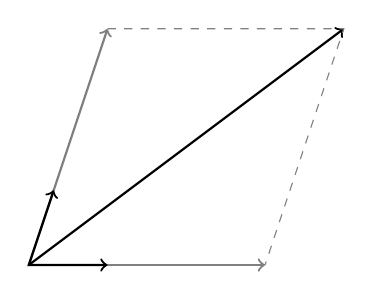
\begin{tikzpicture}
        \draw[->, thick, gray] (0, 0) -- (3, 0);
        \draw[->, thick, gray] (0, 0) -- (1, 3);
        \draw[<->, thick]  (1, 0) -- (0, 0) -- (0.316228, 0.316228 *3);
        \draw[->, thick] (0, 0) -- (4, 3);
        \draw[dashed, gray] (1, 3) -- (4, 3) -- (3, 0);
    \end{tikzpicture}
\end{center}

有了这个定理,在平面上选取了两个不共线的向量$u$,~$v$之后,所有向量就完全由两个实数$a,b$完全决定了。不难发现,我们通常使用的平面直角坐标系,实际上就是取$u=(1,0)$,~$v=(0,1)$的特殊情形。

有这样一个“坐标系”可以帮助我们解决许多问题,我们希望将其推广到任意的线性空间上。幸运的是,我们总是可以做到这一点:对任意数域$F$上的线性空间$V$,存在一族\footnote{为了方便表示,我们使用一个集合$I$中的元素作为下标,但指标集$I$可能是无穷集,也可能不可数。这里的$I$和单位矩阵没有任何关系。}元素$\{e_i\}_{i\in I}$,使得对每一个元素$v\in V$,都存在$i_1,\,\dots\,,i_n\in I$及$x_1,\,\dots\,,x_n\in I$,使得
\[v=x_1e_{i_1}+\cdots +x_ne_{i_n}.\]
同时这种表示是唯一的。此时我们称$\{e_i\}_I$是线性空间的一组基。如果$|I|$是有限的,那么两组基的元素个数是相等的,我们称其为线性空间的维数。

需要注意,我们目前只允许有限个元素进行求和,正如之前在数学分析的部分所介绍的一样。在另外,表示的“唯一性”告诉我们$e_i$之间是线性无关的。也就是说:对一切$i_1,\,\dots\,,i_n\in I$,
\[x_1e_{i_1}+\cdots +x_ne_{i_n}=0\]
当且仅当$x_1=x_2=\cdots =x_n=0$。在平面向量的情形,这相当于说两个向量不共线;在空间向量的情形,这相当于说没有一个向量落在其余两个所在的平面里。

证明向量空间都有基并不是一件简单的事情,比如对连续函数的例子,就很难想象有这样一组基存在。这个证明需要用到与选择公理等价的Zorn引理,初学者可以暂时跳过。但一旦承认了这个结果,我们的许多推理和构造都能方便许多。

接下来,我们集中关心有限维的线性空间,基中元素的个数都是有限的。

除了单独的线性空间之外,我们要在不同的线性空间之间建立起联系。设$V$,~$V'$是$F$上的线性空间,我们考虑映射$f:V\to V'$。我们希望线性空间结构能对研究起到帮助,因此我们要求$f$和线性空间结构“相容”。也即:对一切$u,v\in V$,~$c\in F$
\[f(u+v)=f(u)+f(v),\quad f(cu)=cf(u).\]
上面的等式里,左侧依赖$V$的线性空间结构,而右侧依赖$V'$的线性空间结构。我们称这样的映射为线性映射,如果$V'=V$,我们称其为线性变换,有时也称为$V$上的线性算子。

这些线性映射长什么样?我们可以在熟悉的例子里面考虑,比如平面上的线性变换。我们其实已经见过不少这样的变换:

绕原点$\theta$角的旋转。其公式为
\[(x,y)\mapsto (x\cos\theta+y\sin \theta,-x\sin\theta+y\cos\theta).\]

坐标的“伸缩”变换。对横纵坐标的比例系数$a,b\neq 0$,其规则为
\[(x,y)\mapsto(ax, by).\]

当然还有沿过原点的轴的翻转。比如:

% !
\begin{figure}[h]
    \centering
    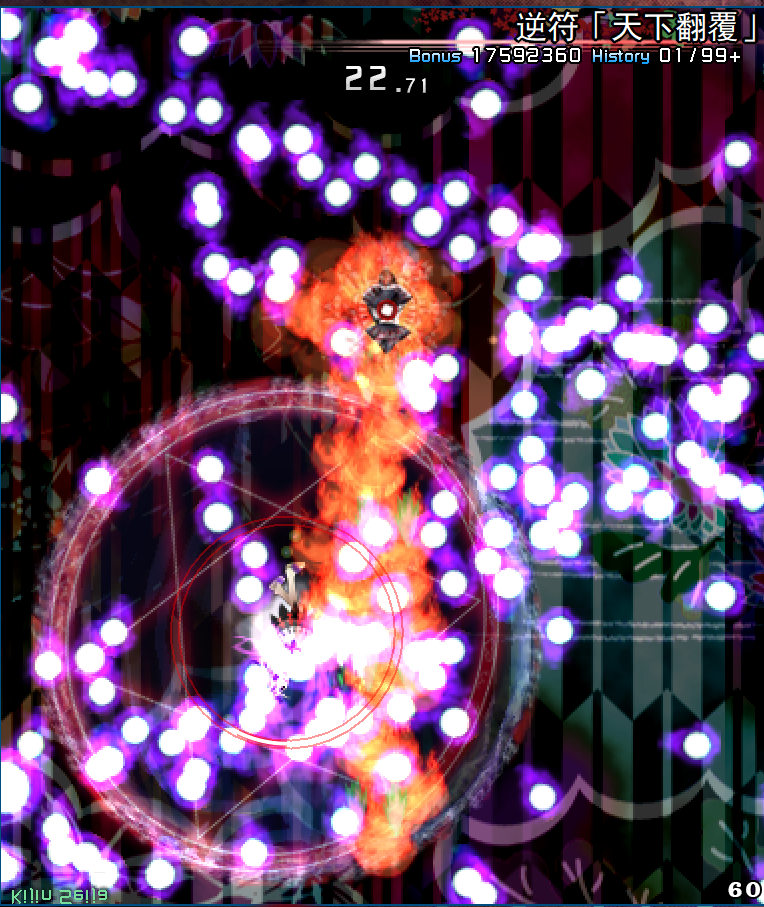
\includegraphics[scale=0.3]{Reflection.png}
\end{figure}

这些都是线性变换的具体例子。不过,平移一般不是线性变换,因为从我们的定义容易看出线性映射将$0$映到$0$。

有了线性映射,选取基的好处就体现出来了。假如有线性空间$U,V$间的线性映射$f:U\to V$,我们选取一组$U$的基$u_1,\,\dots\,,u_n$,由于$U$中每个元素可以被$u_i$线性表出,$f$在$x\in U$的取值被$f$在$u_i$上的取值所唯一确定。

如果我们再为$V$选一组基$v_1,\,\dots\,,v_m$,那么每个$f(u_i)$又被其$v_j$分量的各个“坐标”所确定。这样,刻画这个线性映射只需要$mn$个常数$a_{ij}$,使得
\[f(u_j)=\sum_{i=1}^ma_{ij}v_i.\]
我们将这些常数排成一个$m\times n$(即$m$行$n$列)的表:
\[ A =
    \begin{pmatrix}
        a_{11} & a_{12} & \ldots & a_{1n} \\
        a_{21} & a_{22} & \ldots & a_{2n} \\
        \vdots & \vdots & \ddots & \vdots \\
        a_{m1} & a_{m2} & \ldots & a_{mn} \\
    \end{pmatrix} . \]
我们称之为线性映射$f$在基底$\{u_i\},\{v_j\}$下的矩阵。如果$f$是线性算子,我们通常取$\{v_j\}=\{u_i\}$。

线性映射的结构允许我们进行一些操作。比如两个线性空间之间的两个线性映射可以相加:\[(\;\!f+g)(x)=f(x)+g(x)=g(x)+f(x)=(g+f)(x).\]

线性映射也可以像集合的映射一样进行复合:
\[gf(x)=(g\circ f)(x)=g(f(x)).\]

容易证明这些映射都是线性的。这些线性映射之间的矩阵有何关系?

不难看出,两个线性映射$f_1$,!$f_2$的和$f_1+f_2$的矩阵是$f_1$和$f_2$的矩阵各个分量直接相加,我们称其为矩阵的和。矩阵对求和明显是交换、结合的。加法单位元是分量全为$0$的矩阵,$A$的逆元是与$A$的各个分量乘以$-1$得到的矩阵。

假设$U,V,W$分别是$m,n,p$维的线性空间,其基分别为$\{u_i\},\{v_j\},\{w_k\}$,$f,g,g\circ f$所对应的矩阵是$A,B,C$,那么$A,B,C$分别是$n\times m$,~$p\times n$,~$p\times m$的矩阵。简单的计算可以得出
\[c_{ij}=\sum_{k=1}^nb_{ik}a_{kj},\]
其中$a_{ij}$0,~$b_{ij}$,~$c_{ij}$分别是$A,B,C$在$i$行$j$列的元素。我们定义矩阵$C$为矩阵$B,A$的乘积,记为$C=BA$。映射复合的“结合律”自然给出了矩阵乘法的结合律\footnote{注意矩阵进行乘法时,前一个的列数和后一个的行数必须一致!}。在所有$n\times n$的“方阵”中,矩阵乘法的单位元是单位矩阵:
\[I=I_n=\begin{pmatrix}
        1      & 0      & \ldots & 0      \\
        0      & 1      & \ldots & 0      \\
        \vdots & \vdots & \ddots & \vdots \\
        0      & 0      & \ldots & 1      \\\end{pmatrix}.\]
但即使是对方阵,乘法也未必满足交换律。

通过上面的对应,研究映射的问题就可以被转化成研究矩阵的问题。前者往往是抽象的,而后者往往是具体而可以计算的。
\subsection{线性算子的行列式}
在$\mathbb{R}^n$里面,我们有一种对“体积”的直观感受。而$\mathbb{R}^n$上的线性算子都是“作用均匀”的拉伸变形。我们自然可以考虑一个线性算子下“体积”的变化程度。

我们以平面上的几个线性算子为例。旋转是保持面积和定向的,因此其“体积变化率”是$1$。

沿着过原点某条轴的翻转。面积的大小不变,但是其“定向”被改变了——顺时针会变成逆时针。对“有向体积”来说,这相当于改变了一个符号,因此其“体积变化率”是$-1$。

以$a$,~$b$为比例系数对进行伸缩,和之前的例子相同。此时体积变化率是$ab$。注意当$a=-1$,~$b=1$时,这相当于一个翻转;当$a=b=-1$时,这相当于一个旋转。

怎样在$\mathbb{R}^n$上计算这个体积变化率?我们选取标准基$e_i$为仅有第$i$个分量为$1$,其余均为$0$的元素。在线性算子$T$的作用下,由$e_1,\,\dots\,,e_n$“张成”的高维“立方体”会被映到$T(e_1),\,\dots\,,T(e_n)$张成的“平行多面体”:

\begin{center}
    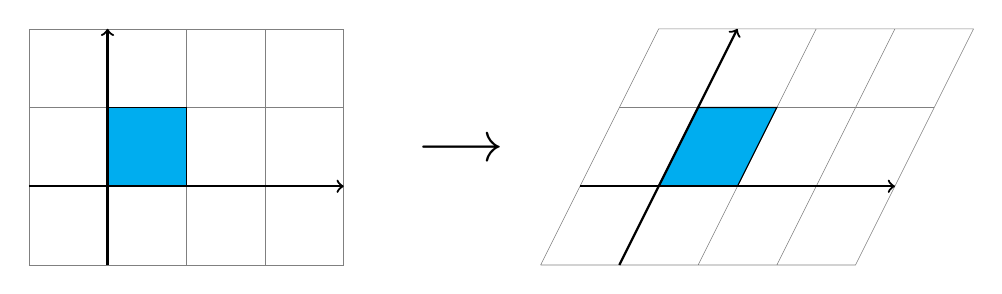
\begin{tikzpicture}
        \draw[step=1cm,gray,very thin] (-1,-1) grid (3, 2);
        \draw[fill = cyan] (0, 0) rectangle (1, 1);
        \draw[thick, ->] (-1, 0) -- (3, 0);
        \draw[thick, ->] (0, -1) -- (0, 2);

        \node at (4.5, 0.5) {\huge\(\longrightarrow\)};

        \draw[xslant = 0.5, xshift = 7cm, step=1cm,gray,very thin] (-1,-1) grid (3, 2);
        \draw[xslant = 0.5, xshift = 7cm, fill = cyan] (0, 0) rectangle (1, 1);
        \draw[xslant = 0.5, xshift = 7cm, thick, ->] (-1, 0) -- (3, 0);
        \draw[xslant = 0.5, xshift = 7cm, thick, ->] (0, -1) -- (0, 2);
        % \draw[cm={0,1,1,0,(1cm,1cm)},red] (0, 0) rectangle (1, 1);
    \end{tikzpicture}
\end{center}

我们将由始于同一点的向量$v_1,\,\dots\,,v_n$张成的平行多面体的(有向)体积记为$\mathrm{vol}(v_1,\,\dots\,,v_n)$。然而,我们还没有定义什么是“体积”!
与之前数学分析中不同,我们面对的是“平行多面体”这类简单的几何对象,中学里的几何直觉仍然发挥着一定的作用。我们按照我们“想象中”的体积提出$\mathrm{vol}$应当满足的几条性质:

首先,“单位立方体”应该具有体积$1$。因此$\mathrm{vol}(e_1,\,\dots\,,e_n)=1$。

延长某一条边会引起体积相应倍数的变化。即对$1\leqslant  i\leqslant  n$,
\[\mathrm{vol}(v_1,\,\dots\,,\,cv_i,\,\dots\,,v_n)=c\cdot \mathrm{vol}(v_1,\,\dots\,,v_n),\]
其中$c$是任意实数,可以为$0$或负数。当$c=0$,这个平行多面体被“拍扁”成了一个低维的平面,从而体积为$0$;当$c$为负值,我们改变了整个平行多面体的定向,从而体积反号。

我们知道“同底等高”的平行四边形面积是相等的。也就是说,$v_1$,~$v_2$张成的平行四边形和$v_1+c\cdot v_2$,~$v_2$张成的平行四边形面积相等。这可以推广到高维情形:对一切$1\leqslant  i,j\leqslant  n$,~$i\neq j$,
\[\mathrm{vol}(v_1,\,\dots\,,\,v_i+c v_j,\,\dots\,,v_n)=\mathrm{vol}(v_1,\,\dots\,,v_n).\]
可以证明,有了上面几条性质,函数$\mathrm{vol}$就被唯一地确定了。给定$V$上的一个线性算子$T$,可以证明当$\mathrm{vol}(v_1,\,\dots\,,v_n)\neq 0$时,
\[\frac{\mathrm{vol}(Tv_1,\,\dots\,,Tv_n)}{\mathrm{vol}(v_1,\,\dots\,,v_n)}\]
是一个定值。我们将其称为线性算子的行列式,记为$\det T$。

按照我们的定义方式,容易看出:恒等映射的$\mathrm{det}$是$1$,对两个线性映射$T,T'$,复合映射的“体积变化率”等于两个“体积变化率”的乘积:
\[\det T\det T'=\det TT'.\]
由于线性算子的行列式与基的选取无关,我们可以取线性算子在任一组基下的矩阵
\[A =
    \begin{pmatrix}
        a_{11} & a_{12} & \ldots & a_{1n} \\
        a_{21} & a_{22} & \ldots & a_{2n} \\
        \vdots & \vdots & \ddots & \vdots \\
        a_{n1} & a_{n2} & \ldots & a_{nn} \\
    \end{pmatrix}. \]
那么,我们可以从矩阵$A$算出$\det T$的表达式:
\[\det T=\sum_{\sigma}\mathrm{sgn}(\sigma)a_{1\sigma(1)}\cdots a_{n\sigma(n)},\]
其中$\sigma$取遍所有$\{1,\,\dots\,,n\}$到自身的双射,而$\mathrm{sgn}(\sigma)$表示$\sigma$的符号。将$\sigma$表示成一些对换\footnote{即只有两个元素互换位置的置换。}的复合时,设对换的个数为$l$,那么$\mathrm{sgn}(\sigma)=(-1)^l$。由这个公式,我们可以谈论一个矩阵$A$的行列式$\det A$。

行列式可以告诉我们$V$上的一个线性算子$T$是不是可逆的,即是否存在另一个线性算子$T^{-1}$,使得$TT^{-1}=T^{-1}T$是$V$上的恒等映射$\mathrm{id}_V$。

如果一个线性算子$T$具有行列式$0$,即“体积变化率”是$0$,那么$T$将“全空间”$V$压缩到一个维数较低的“平面”$W$上,但$W$的一组基比$V$的一组基元素个数要少,因此$W\to V$无论怎么映射都不可能是满射,故而不可逆。

反过来,如果$\det T\neq 0$,那么$T$将一组基打到一组线性无关的元素。由于所有的基元素个数都相同,这些元素可以张成整个$V$,所以也是一组基。由此得出$T$是可逆的。
\subsection{换基与特征向量}
要谈论线性映射的矩阵,前提是取好线性空间上的基。但是一个线性空间上基的选取有很多种方式,不同的选取方式会得到不同的矩阵。那么,这些矩阵之间有什么关系呢?

利用我们之前建立的矩阵乘法和线性映射复合的关系,很容易得到答案。假设$f:U\to V$是有限维线性空间之间的线性映射,在$U$上取两组基$\{u_i\}_{1\leqslant  i\leqslant  n}$和$\{u_i'\}_{1\leqslant  i\leqslant  n}$,在$V$上取两组基$\{v_j\}_{1\leqslant  j\leqslant  m}$和$\{v_j'\}_{1\leqslant  j\leqslant  m}$。我们设$A$,~$A'$是$f$在基底$\{u_i\}$,~$\{v_j\}$和$\{u_i'\}$,~$\{v_j'\}$下的矩阵。注意到,$f$可以表示为一个复合
\[\mathrm{id}_V\circ f\circ \mathrm{id}_U,\]
其中$\mathrm{id}_V:V\to V$和$\mathrm{id}_U:U\to U$是$V,U$到自身的恒等映射。

现在,我们在$\mathrm{id}_U$的定义域里使用基$\{u_i'\}$,值域里使用基$\{u_i\}$,得到$\mathrm{id}_U$的矩阵记为$Q$;在$\mathrm{id}_V$的定义域里使用基$\{v_j\}$,值域里使用基$\{v_j'\}$,得到$\mathrm{id}_V$的矩阵记为$P$。注意,虽然这些都是恒等映射,但我们在定义域和值域上选的不是同一组基,因此$P,Q$一般不是单位矩阵。

经过复合,我们就得到 $f$ 在 $\{u_i'\}$,~$\{v_j'\}$ 下的矩阵$A'=PAQ$。

当然,我们也可以更具体地描述$P$,~$Q$。按照定义,若
\[u_i'=\sum_{k=1}^nq_{ki}u_{k},\]
\[v_j=\sum_{l=1}^mp_{lj}v_l'.\]
那么$P$,$~Q$分别是$p_{lj}$,~$q_{ki}$作为下标对应位置分量的矩阵。

在研究线性算子时,我们通常在定义域和值域选取同样的基,
此时$P$,~$Q$之间也是有关联的。可以发现,$PQ$,~$QP$都是定义域和值域使用相同的基时,恒等映射对应的矩阵。从而
\[PQ=QP=I.\]
也即$Q=P^{-1}$,$A'=PAP^{-1}$。我们称两个矩阵$A$,~$B$相似,当且仅当存在互逆的矩阵$P$,~$P^{-1}$,$B=PAP^{-1}$。

设$p$是在基底$\{u_i\}$下以$P^{-1}$为矩阵的线性算子,$P^{-1}$的可逆性确保$p(u_i)$成为一组基。那么,将基底由$u_i$换成$p(u_i)$后,原先以$A$为矩阵的线性算子将会以$PAP^{-1}$作为新的矩阵。因此,相似矩阵不过是同一个线性算子在不同的基下的矩阵。

给定一个线性算子$T$,我们总是希望让其矩阵尽可能地简单。比较简单的一类矩阵是对角矩阵:
\[\mathrm{diag}(\lambda_1,\,\dots\,,\lambda_n)=\begin{pmatrix}
        \lambda_1 & 0         & \ldots & 0         \\
        0         & \lambda_2 & \ldots & 0         \\
        \vdots    & \vdots    & \ddots & \vdots    \\
        0         & 0         & \ldots & \lambda_n \\\end{pmatrix}.\]
要将矩阵通过相似化成这个形状,就是要找到基$e_i$使得$T(e_i)=\lambda_ie_i$。

这些$\lambda_i$是什么?我们注意到$(T-\lambda_i\mathrm{id})(e_i)=0$,从而$T-\lambda_i\mathrm{id}$是不可逆的。设在一组基下$T$有矩阵$A$,我们考虑
\[\det (T-\lambda\mathrm{id})=\det(A-\lambda I),\]
这是一个关于$\lambda$的$n$次多项式,称为$T$的特征多项式。所有$\lambda_i$必然是这个多项式的根。

如果特征多项式有$n$个不同的根$\lambda_1,\,\dots\,,\lambda_n$,事情进展得非常顺利:由于$T-\lambda_i\mathrm{id}$不可逆,可以找到$v_i\neq 0$使得$(T-\lambda_i\mathrm{id})(v_i)= 0$。此时可以证明$v_i$线性无关,从而$v_i$构成了我们想要的基。

但,当特征多项式有重根或者有不可约的高次因式(比如实数上的二次不可约多项式),就没有那么顺利了。我们尚可以做两方面的努力:或者假定矩阵的形状比较好,或者假定数域$F$的性质比较好。

对于前者,可以证明:如果一个实数方阵是对称的,即$i$,~$j$位置和$j$,~$i$位置的分量相等,那么这个方阵可以在相似下被化成对角的形式。

至于后者,我们通常要求$F$代数闭——即系数落在$F$中的方程,根也全在$F$中。根据代数学基本定理,$\mathbb{C}$就是这样的一个例子。此时,任何矩阵都可以通过相似化为下面的形式(空白处以$0$填充):
\[
    \begin{pmatrix}
        J_{n_1}(\lambda_1) &                    &        &                    \\
                           & J_{n_2}(\lambda_2) &        &                    \\
                           &                    & \ddots &                    \\
                           &                    &        & J_{n_k}(\lambda_n) \\\end{pmatrix}.
\]
其中每个$J_{n_i}(\lambda_i)$是小块的$n_i\times n_i$矩阵,称为Jordan块。其形如
\[J_{n_i}(\lambda_i)=
    \begin{pmatrix}
        \lambda_i & 1         &        & \ldots    & 0         \\
        0         & \lambda_i & 1      &           & \vdots    \\
        \vdots    & \vdots    & \ddots & \ddots    &           \\
        0         & 0         & \ldots & \lambda_i & 1         \\
        0         & 0         & \ldots & 0         & \lambda_i \\\end{pmatrix}.
\]
同时,这些Jordan块精确到置换是唯一的。

现在我们将上面的概念应用到具体的问题里,比如解线性方程组。我们先来考虑齐次的线性方程组
\[
    \begin{cases}
        a_{11}x_1+a_{12}x_2+\cdots+a_{1n}x_n=0, \\
        a_{21}x_1+a_{22}x_2+\cdots+a_{2n}x_n=0, \\
        \mathord{\cdots}\mathord{\cdots}        \\
        a_{m1}x_1+a_{n2}x_2+\cdots +a_{mn}x_n=0.
    \end{cases}
\]
利用矩阵乘法,我们可以将其写为简洁的形式:
\[AX=0.\]
其中
\[A = \begin{pmatrix}
        a_{11} & a_{12} & \ldots & a_{1n} \\
        a_{21} & a_{22} & \ldots & a_{2n} \\
        \vdots & \vdots & \ddots & \vdots \\
        a_{m1} & a_{m2} & \ldots & a_{mn} \\
    \end{pmatrix},\quad
    X = \begin{pmatrix}
        x_1    \\
        x_2    \\
        \vdots \\
        x_n    \\
    \end{pmatrix}.\]

我们可以重新理解“解方程组”:$V,W$分别是全体$n\times 1$矩阵和全体$m\times 1$构成的线性空间,线性映射$f:V\to W$将$X$映至$AX$。设$e_i$,~$f_i$分别是$V,W$中仅有第$i$行元素为$1$,其余元素均为$0$的矩阵,那么$f$在基$\{e_i\},\{\;\!f_j\}$下的矩阵由$A$给出。解这个方程组,就是要寻求$V$的子空间$U$:
\[U=\bigl\{\,v\in V\mid\, f(v)=0\,\bigr\}.\]

如果$A$的形状比较特殊,比如非$0$部分呈现“倒阶梯状”,那么解方程组是比较容易的事情:把下面的部分解出来,再代入上方就可以了。但对于一般的方程,解起来就没有那么容易。

怎么改变矩阵的形状呢?

虽然$\mathrm{id}_U$,~$\mathrm{id}_V$是恒等映射,但由于我们在定义域和值域选了不同的基,其矩阵通常不是
以$a_{ij}$和$a_{ij}'$表示矩阵$A$,~$A'$在$i$行$j$列处的分量。
按照定义,$a_{ij}$和$\{a_{ij}'\}$依照下面方式确定:
\[
    f(u_j)=\sum_{i=1}^ma_{ij}v_i,\quad f(u_j')=\sum_{i=1}^ma_{ij}'v_i'
    .\]
由于$\{u_i\},\{u_i'\}$都是基,这两组基可以相互表出。我们设
\[
    u_i'=\sum_{k=1}^nb_{ki}u_{k}
    ,\]
\[
    v_j=\sum_{l=1}^mc_{lj}v_l'
    .\]
那么,可以得到
\begin{align*}
    f(u_i') & =\sum_{k=1}^nb_{ki}f(u_k)
    =\sum_{k=1}^nb_{ki}\sum_{s=1}^ma_{sk}v_s                           \\
            & =\sum_{s=1}^m\left( \sum_{k=1}^na_{sk}b_{ki} \right) v_s
    =\sum_{j=1}^m\left( \sum_{s=1}^m\sum_{k=1}^nc_{js}a_{sk}b_{ki} \right) v_j'.
\end{align*}
从而$A'$在$i$行$j$列的分量是$\sum_{s=1}^m\sum_{k=1}^nc_{ls}a_{sk}b_{ki}$。如果我们以$B,C$分别表示以$b_{ij}$,~$c_{ij}$作为$i$行$j$列分量的矩阵,利用矩阵乘法可以将$A'$表示为$CAB$.
%一个计数器

\newtcolorbox{abox}[1][]{
	enhanced,
	blanker,
	top = 0mm,
	bottom = 0mm,
	sharp corners,
	fontupper = \footnotesize\itshapeCJK,
	colframe = black,
	boxsep = 0pt,
	width = 3cm,
	left = 5pt,
	right = 5pt,
	borderline west = {\ifodd\value{page}1pt\else 0pt\fi}{0pt}{\ifodd\value{page}black\else white\fi},
	borderline east = {\ifodd\value{page}0pt\else 1pt\fi}{0pt}{\ifodd\value{page}white\else black\fi},
	unbreakable,
	before upper = {\setlength{\lineskip}{5pt}%
			\setlength{\lineskiplimit}{2.5pt}\setlength{\parskip}{0.5em}}
}


\begin{center}
	\chapter[幻想乡工程技术见闻录 \~{} Fantasy from Triviality]{幻想乡工程技术见闻录 \~{} Fantasy from Triviality}
\end{center}
\begin{flushright}
	\large{\textbf{——力学专业概貌及基础数学介绍}}
\end{flushright}

\addauthor{山舞银蛇 \& 小麻雀}


\section*{前言}

 {\itshapeCJK
  无论从理科还是工科的视角来看,力学都是十分重要的基础学科。然而就笔者的经验来看,目前国内很多高校要么没有开设力学专业导论课,要么很难起到引导学生认识力学、形成审视力学学科观点的作用,只片面地介绍一些前沿热点问题。此外,力学专业课和数理基础课之间也存在脱节情况,目前国内已有高校认识到这一点,并尝试组织课改。笔者针对以上两点问题,以个人经历及所见所知,参考一些权威的观点和资料,写下了这份手册。

  笔者始终信奉一个观点:有些东西不必刻意追求,当你所做的工作充分时,这些东西就是唾手可得的。在“本科高中化”趋势日益明显的大环境下,只有将所学的内容有机地结合、串联在一起,才能不囿于“内卷”这个小圈子,让学习、科研变得事半功倍。要想做到将所学的专业知识组织在一起,能够把握专业的概貌绝对是一个必要条件,而这一环往往又是大家容易忽视的。

  本手册的初衷是起到补全当前力学学科教育中缺失环节的辅助作用,所涉及的内容都是力学及相关数学的基础内容,只有少量笔墨涉及相对高级的数学工具。不会花费大量篇幅阐述力学的前沿热点问题和高级数学工具的具体内容,也不会教授应试技巧,更不是所谓的“速通”或“速成”手册。我们旨在给力学及相关专业的大一、大二新生呈现力学专业的概貌,了解力学学科做过和要学什么,以及对数学基础及其力学应用有一个初步的认识,在此基础上逐渐形成对力学专业的宏观把握,最终起到使得读者能够快速入门力学的某个具体分支的作用。

  这份手册大致分为两个部分,前一部分对力学作一个概述,从力学的历史出发,介绍力学的主要研究内容和研究方法;后一部分针对的是力学的数学基础,对如何学习和应用力学的数学工具提出建议。当然,对于新生来说,这其中必然涉及一些此前不曾听说过的名词和概念,给阅读增添障碍,我们希望读者通过阅读手册的内容能够独立地破除这个障碍。我们希望读者能在学习新的力学和数学知识后反复审视一些内容,其实不光这本手册是这样,做学术研究也应该这样,水平提高后返璞归真,可能会有新的体会与收获。

  八云的魔法书社团活动的基础是东方project系列和数学,然而我们不得不承认在融合这二者这一点上,我们做得并不够好。为了调和二者兼容性的矛盾,笔者产生了用故事的形式呈现这些知识的想法,当然这里的故事并不是此前简单缝合的模式,而是一个剧情、逻辑足够完整的故事。然而由于时间限制,我们无法在今年新生的适应期完成故事的创作,只好先将我们所想的干货内容整理出来,呈现给大家,还望大家能够用充分的耐心等待完整作品的问世!

  由于编者的学识水平有限,加之时间紧张,手册中难免出现纰漏和错误,还望读者与同行能够指出错误,让我们一同进步和成长!
 }

\begin{flushright}
	八云的魔法书\\
	新生手册编写-力学及其数学小组\\
	2022.11.06
\end{flushright}

\newgeometry{marginparwidth = 2.8cm, marginparsep = 0.5cm, outer = 5.9cm, top=1.16in, bottom=1.34in, inner=1.2in}

\section{力学概述}

{\itshapeCJK
    我们在中学阶段学习的物理,以力学和电学为重点,特别是力学。我们对滑块、小球、圆形轨道等物理模型十分熟悉。但是由于所学知识特别是数学工具的限制,刚刚中学毕业的我们还不能很好地认识力学。在中学阶段,我们通常会认为力学是物理的一个分支,并且由于尚未接触微积分等工具,当时的我们只能考察物体以质点模型为基础的简单运动。实际上,力学研究的对象远不止于此,而且力学和物理学已经沿着完全不同的画风发展一个世纪多了,业已取得了相当丰硕的成果,特别是在工程当中获得了广发的应用。

接下来,让我们从力学的发展史出发,简要地了解一下力学的研究内容、分支以及研究方法。
}

\subsection{力学的发展历史}

力学的内容十分丰富,不是三言两语能够讲清楚的,在概括其发展史时当然也面临这个问题,所以我们接下来的介绍只选择了力学发展中比较重要的主干事件。

\begin{marginparfigure}
    \centering
    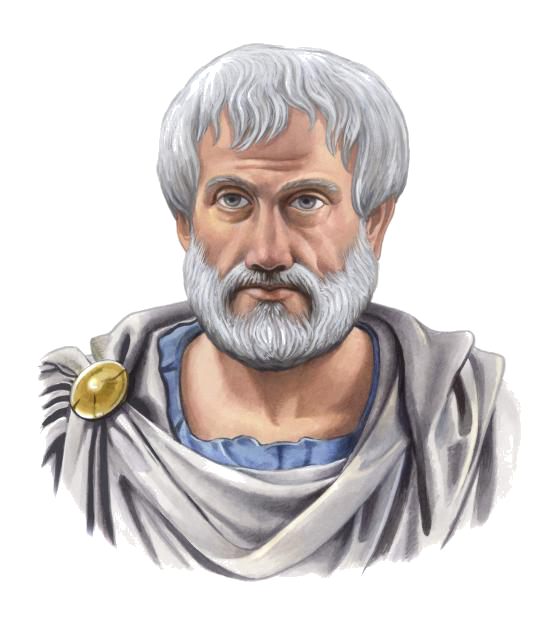
\includegraphics[width = 2.8cm]{Aristotle.png}
    \captionof{figure}{亚里士多德像}
\end{marginparfigure}


\subsubsection{古典时代}

最初,物理学跟力学几乎是同义词。古时候,世界各地的劳动人民就已经在经验上总结许多自然运行的原理,但我们说现代科学的源头在古希腊,因为只有古希腊诞生了形式逻辑与演绎推理,这是数学学科的基础,而一切现代科学又都是建立在形式逻辑、演绎推理与数学描述上的。这里我们介绍一些古希腊时代的著名科学家。

\uwave{亚里士多德}是世界上最伟大的古希腊哲学家与科学家之一,他的研究涉猎广泛,特别是构建了一套影响深远认知系统。尽管亚里士多德的诸多科学结论是错的,却无法掩盖其对现代科学的伟大贡献。


\begin{marginparfigure}
    \centering
    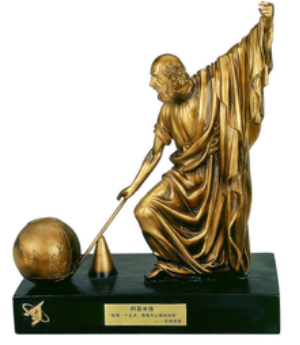
\includegraphics[width = 2.8cm]{Archimedes.png}
    \captionof{figure}{阿基米德像}
\end{marginparfigure}

\uwave{阿基米德}是古希腊最重要的数学家、物理学家之一。一般认为阿基米德是刚体静力学和流体静力学的奠基人,他曾经研究过许多数学和力学问题,如球体积公式、抛物线弓形面积、确定物体重心的方法、物体浮力的计算公式、杠杆原理等。阿基米德曾基于杠杆原理给出一个著名的论断,“给我一个支点,我能撬动地球”。

\begin{marginpartext}
        用如今的观点看,“本轮-均轮模型”是用Fourier级数的方法逼近任意曲线的过程。但若要使逼近足够精确,需要在均轮上添加足够多的“轮上轮”以增加准确性,这正是该体系的繁琐之处。
\end{marginpartext}

此外,阿基米德还制造了许多机械,如螺旋提水机、抛石机等。

\begin{figure}
    \centering
    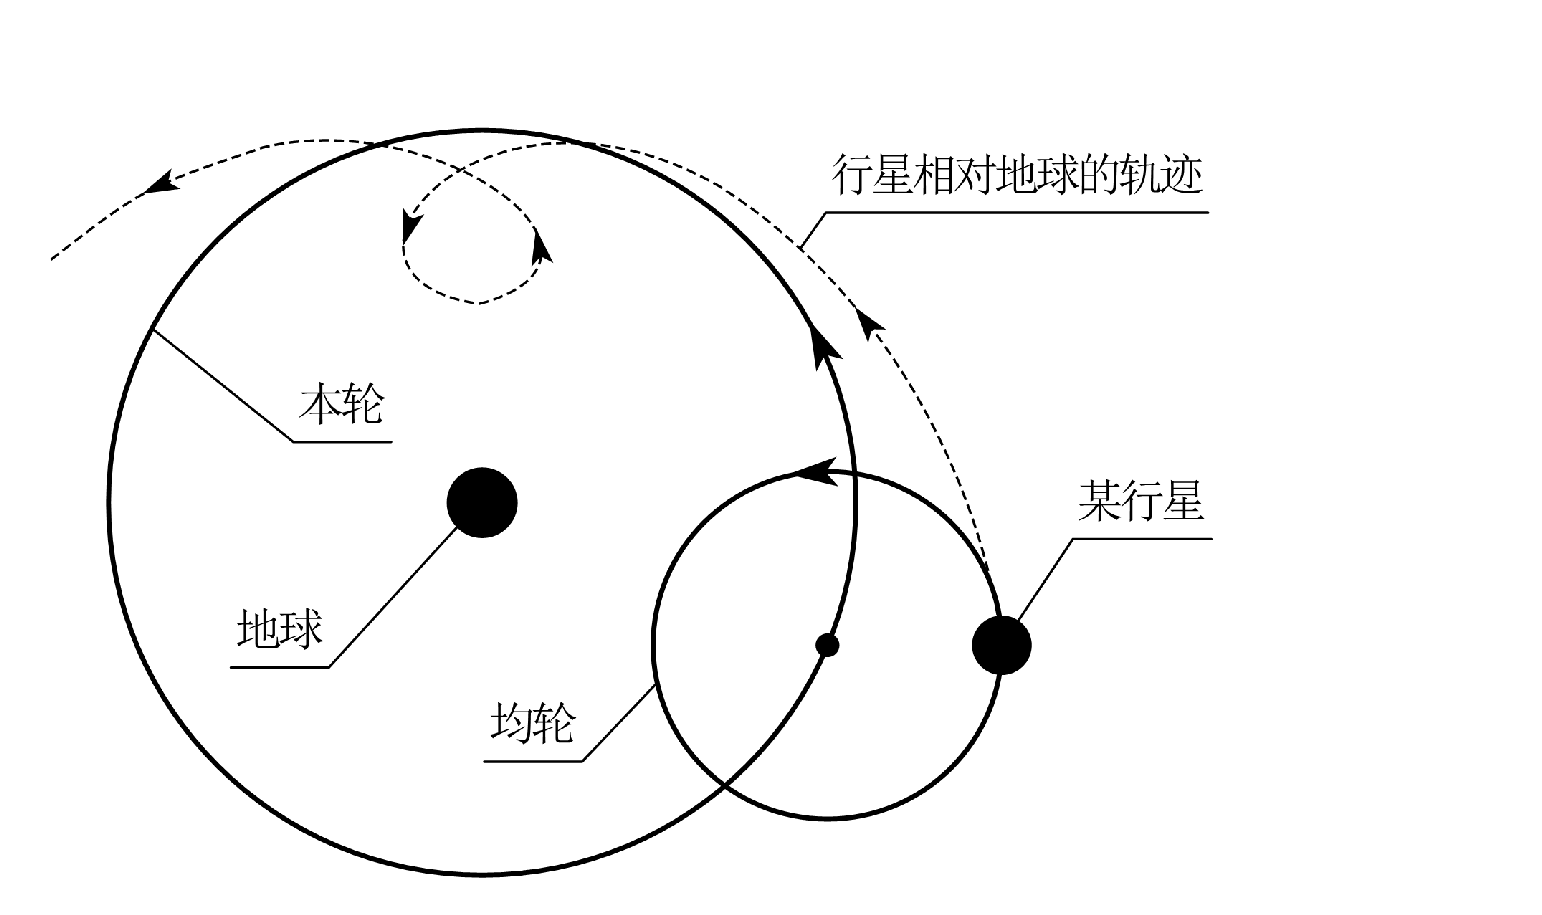
\includegraphics[width = 10.8cm]{epicycle_deferent.pdf}
    \caption{本轮-均轮模型示意}
\end{figure}

古希腊天文学的集大成者是\uwave{托勒密},他认同“地心说”,并且采用\textbf{本轮-均轮模型}来解释行星的运动。托勒密体系的观测精度满足了那个时代的要求,同时“地心说”被认为符合基督教的教义,因而这套体系统治了西方世界1000多年,直到文艺复兴时期才被推翻。

这个时期,由于数学工具还比较初等,微积分等近代数学工具还没出现。尽管阿基米德已经有微积分的思想萌芽,但毕竟不成体系,要系统研究运动学和动力学存在很大困难。所以力学的研究被限制在比较简单的范畴,主要是静力学和比较简单的运动学。

\subsubsection{力学奠基时代}

文艺复兴时期,古希腊的知识得到复兴,各个学科都呈现出一片繁荣景象,新思想和观点的碰撞,使得人们对客观世界的认识有了很大的进步。\uwave{达·芬奇}是文艺复兴时期科学和工程技术领域最重要的人物之一,他提出了许多领先于他那个时代的观点,设计了许多机械图纸,并且还主持修建了诸多水利工程。可以说,达·芬奇揭开了那个科学技术快速发展时代的序幕。

\begin{figure}[ht]
    \centering
    \begin{subfigure}[t]{0.4\textwidth} \centering
        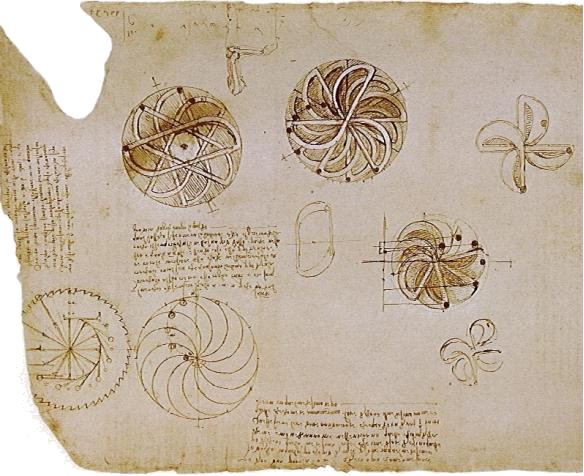
\includegraphics[height = 0.7\linewidth]{daVinci_s.png}
        \caption{达·芬奇的手稿}
    \end{subfigure}\quad
    \begin{subfigure}[t]{0.4\textwidth} \centering
        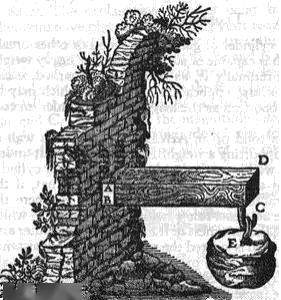
\includegraphics[height = 0.7\linewidth]{Galileo_s_beam.png}
        \caption{伽利略的悬臂梁模型}
    \end{subfigure}\bigskip
\end{figure}



\uwave{伽利略}是“近代科学之父”,
\begin{marginparfigure}
    \centering
    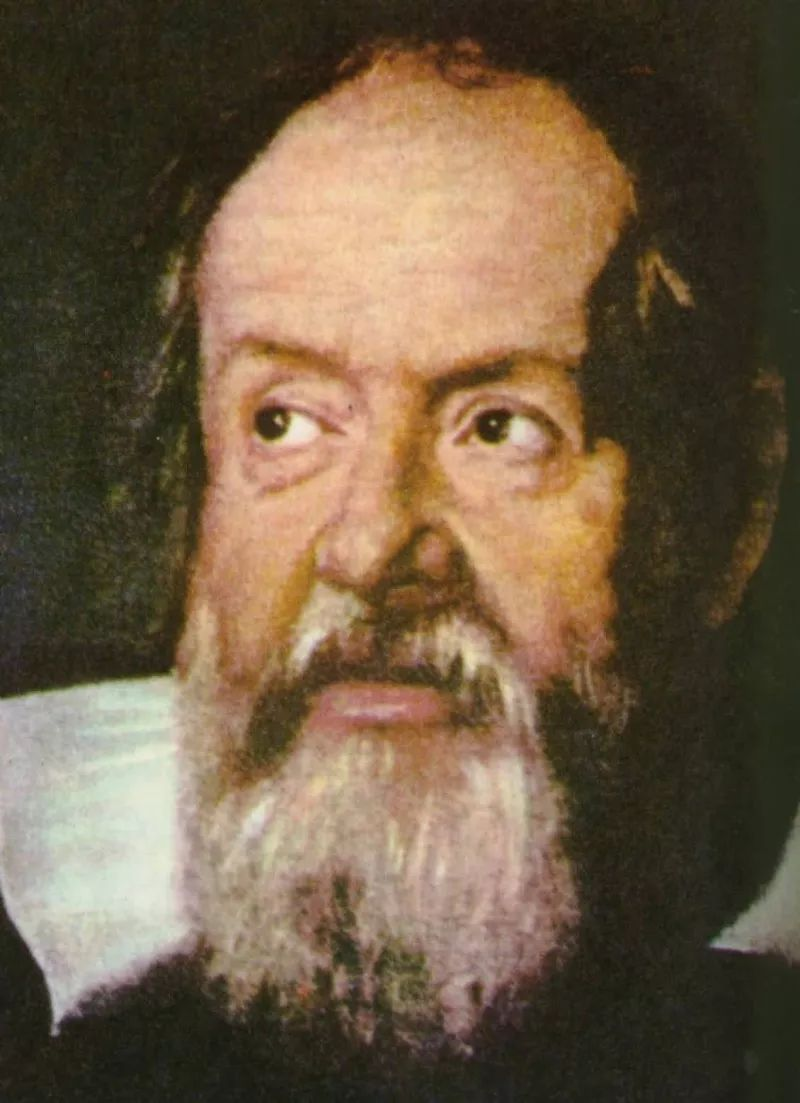
\includegraphics[width = 2.8cm]{Galileo.jpeg}
    \captionof{figure}{伽利略像}
\end{marginparfigure}
他开创了系统科学试验与观察的先河,这种实证精神一直延续到今天的科学研究中。伽利略对于力学和天文学的贡献很大,他首次定量地提出“加速度”的概念,奠定了动力学研究的基础;最早给出了惯性定律;给出了参考系、\textbf{伽利略变换}、相对性原理等概念;另外,伽利略还讨论了悬臂梁变形问题。

\uwave{开普勒}基于其老师第谷的天文观测数据,总结并提出了关于\textbf{行星运动的三大定律},这三条定律为牛顿最终创立经典力学体系奠定了基础。

\begin{figure}[ht]
    \centering
    \begin{subfigure}[t]{0.4\textwidth} \centering
        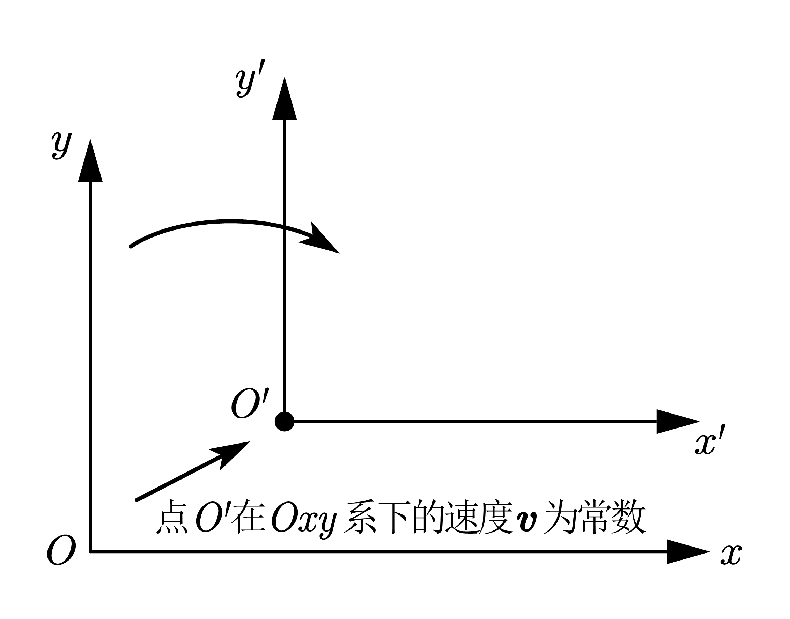
\includegraphics[height = 0.7\linewidth]{Galileo_trans.pdf}
        \caption{伽利略变换}
    \end{subfigure}\quad
    \begin{subfigure}[t]{0.4\textwidth} \centering
        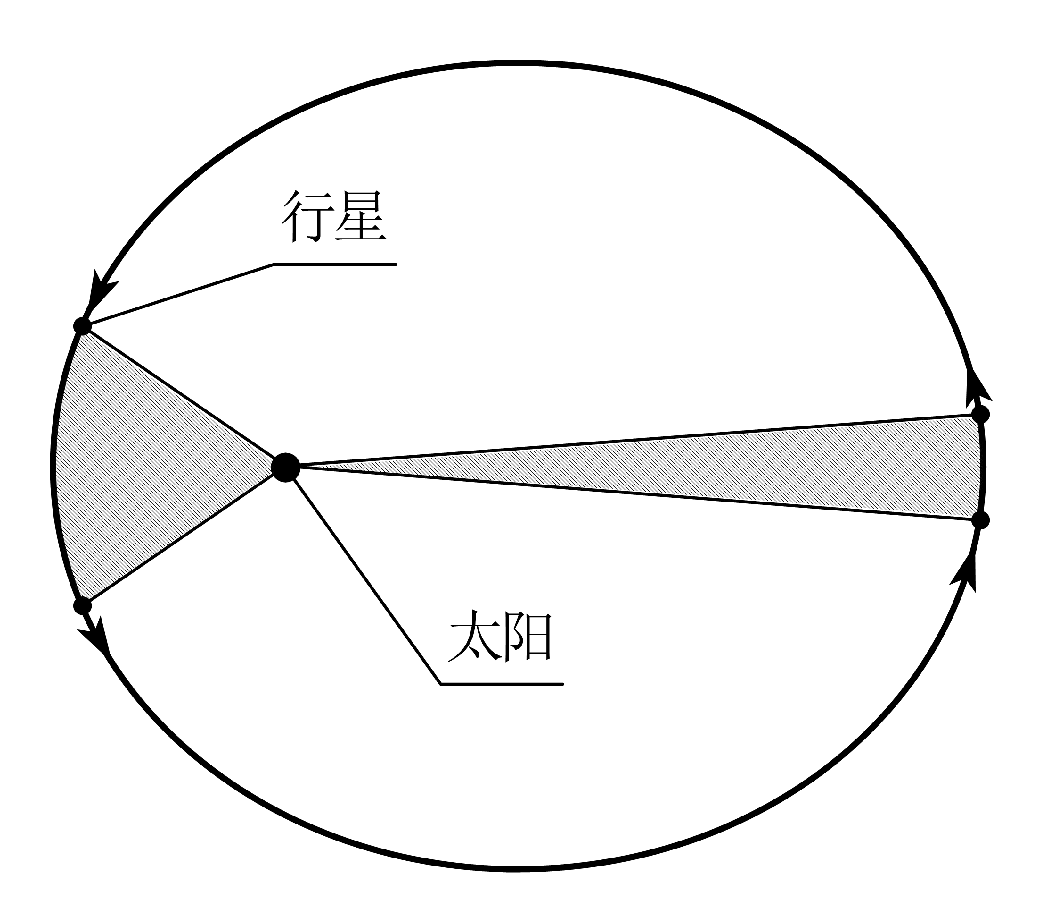
\includegraphics[height = 0.7\linewidth]{Kepler_2.pdf}
        \caption{开普勒第二定律示意}
    \end{subfigure}
\end{figure}

最终创立经典力学体系的工作是由\uwave{牛顿}
\begin{marginparfigure}
    \centering
    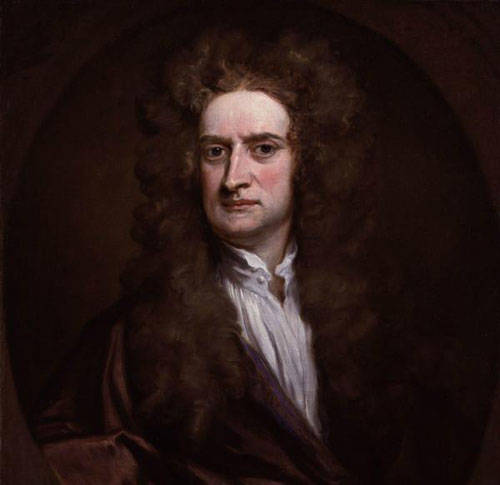
\includegraphics[width = 2.8cm]{Newton.jpg}
    \captionof{figure}{牛顿像}
\end{marginparfigure}在总结前人工作成果的基础上完成的。首先,牛顿总结出了\textbf{牛顿三定律},描述物体运动,这些内容大家十分熟悉,就不再阐述了。其次,牛顿研究了万有引力,最终正确地给出了\textbf{万有引力定律}的数学表达式。牛顿的《自然哲学的数学原理》总结了他所做的大部分力学相关的工作,标志着经典力学体系的成熟。牛顿能取得这些成绩的一个关键因素是他发明并采用了微积分的语言来描述,这是与他同时代许多采用几何观点研究力学的学者所不同的地方。微积分这一数学工具极大地拓展了数学能够描述的物理问题的范围,从这里开始,人们广泛地应用微分方程描述物理规律,再加以求解,成为了定量研究问题的一套范式。

这个时期。还有许多其他著名的学者,如\uwave{惠更斯}、\uwave{胡克}、\uwave{托里拆利}等人,他们在经典力学奠基的阶段也做出了重要的贡献,限于篇幅我们不一一介绍。

\subsubsection{力学进一步发展的时代——分析力学}

接下来力学的发展可以用两条线索概括,其一是经典力学理论进一步发展,得到分析力学体系;其二是对连续介质力学,即固体力学和流体力学的研究。

在牛顿之后,经典力学得到进一步发展。当时的科学家们总结出了诸多定律,守恒定律包括动量、角动量(动量矩)、能量守恒定律;\uwave{达朗贝尔}提出了\textbf{达朗贝尔原理},在非惯性系中添加了“惯性力”,使得能用静力学的手段处理动力学问题;\uwave{约翰·伯努利}首次给出了\textbf{虚功原理}的表述。同时,数学工具得到了进一步发展,对于最速降线问题的讨论导致了变分法这一数学工具的产生,这也标志着分析学正式成为数学的一大分支。


\begin{figure}[ht]
    \centering
    \begin{subfigure}[t]{0.4\textwidth} \centering
        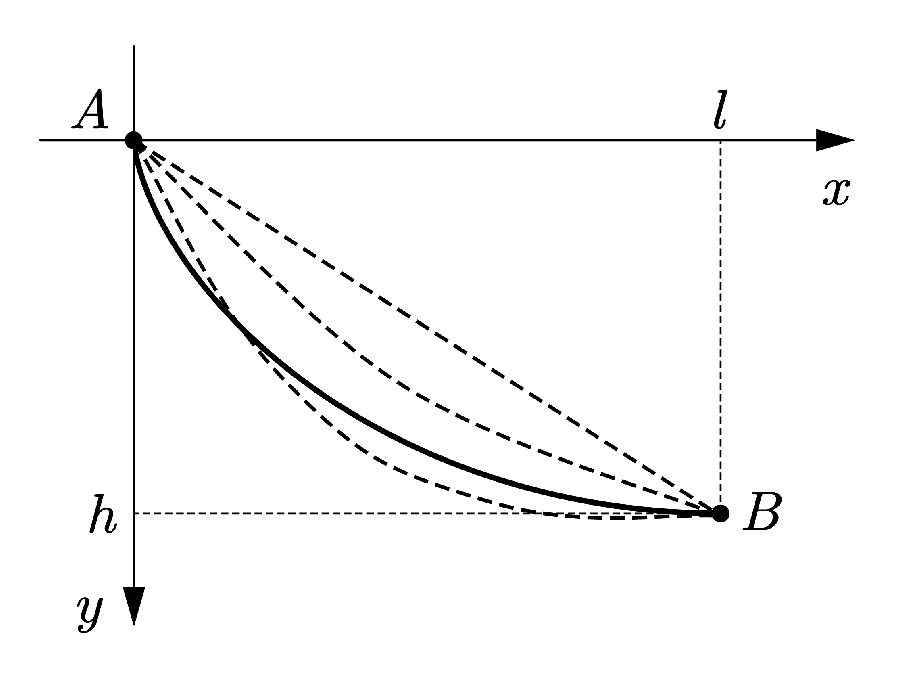
\includegraphics[height = 0.7\linewidth]{cycloid.pdf}
    \end{subfigure}\quad
    \begin{subfigure}[t]{0.4\textwidth} \centering
        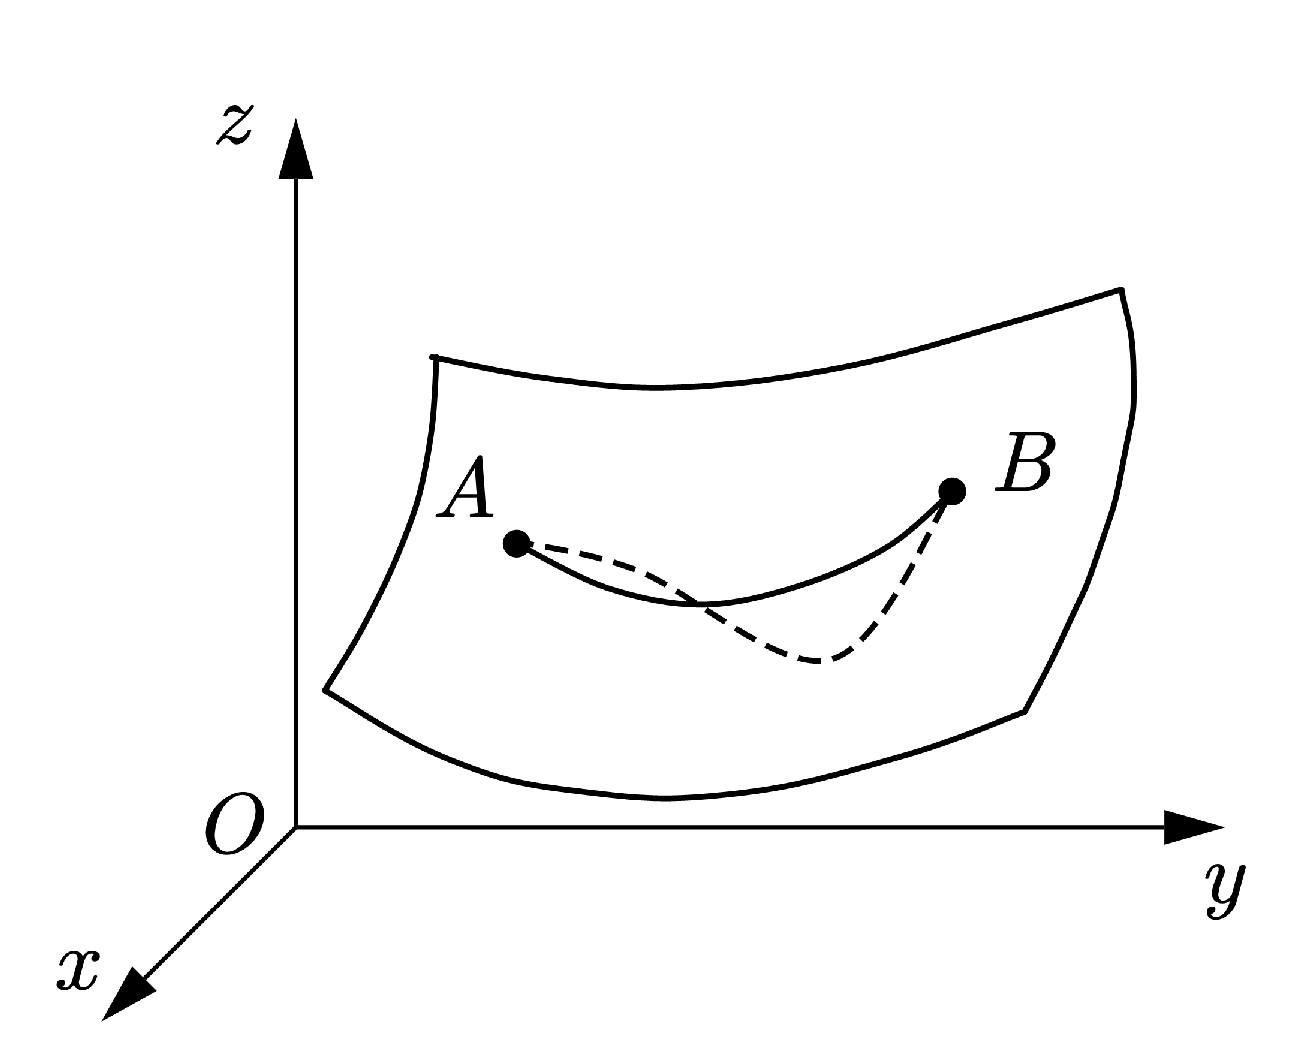
\includegraphics[height = 0.7\linewidth]{geodesic.pdf}
    \end{subfigure}
    \caption{最速降线和曲面短程线问题,对此类泛函极值问题的研究促进了变分法的发展}
\end{figure}
\begin{marginpartext}
    最速降线问题的提法是:设$A$和$B$是铅直平面上不在同一铅直线上的两点,在所有连接$A$和$B$的平面曲线中,求一条曲线,使得仅受重力作用且初速度为零的质点从$A$点沿其运动到$B$点所需时间最短。
\end{marginpartext}

尽管经典力学已经建立起来了,但它还是只能处理简单的质点问题,无法处理刚体(考虑物体的尺寸、形状,并认为物体不会发生变形,与质点相比,存在转动如何描述的问题)这样需要考虑物体形状的问题。同时,牛顿的经典力学理论上能处理有约束的问题,但实际问题过于复杂,用牛顿体系处理并不方便。在这种背景下,分析力学建立起来并得到了发展。

\begin{marginparfigure}
    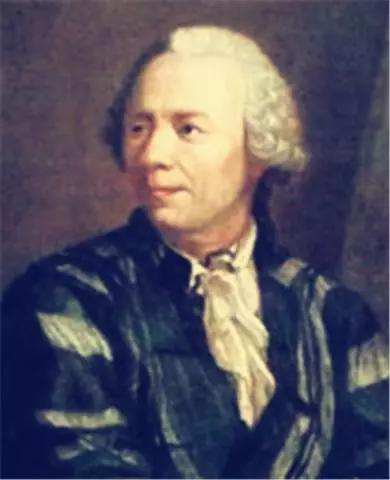
\includegraphics[width = 2.8cm]{Euler.jpg}
    \captionof{figure}{欧拉像}
\end{marginparfigure}

\uwave{欧拉}首先研究了刚体的运动规律,扩大了经典力学能够处理的问题的范畴,而且在这个过程中,产生了\textbf{自由度}的概念,即完整的描述一个力学系统的运动情况所需的最少的变量数。例如,若要完整描述平面刚体的运动速度,只需要知道刚体上任意一点的速度(矢量)及其转动的角速度。自由度的概念是分析力学建立的基础,因而十分重要。此外,欧拉给出了极值曲线、等周问题的解答,创立了变分学,并富有创见性地提出“分析学具有重构牛顿力学体系的潜力”。

\begin{figure}[ht]
    \centering
    \begin{subfigure}[t]{0.4\textwidth} \centering
        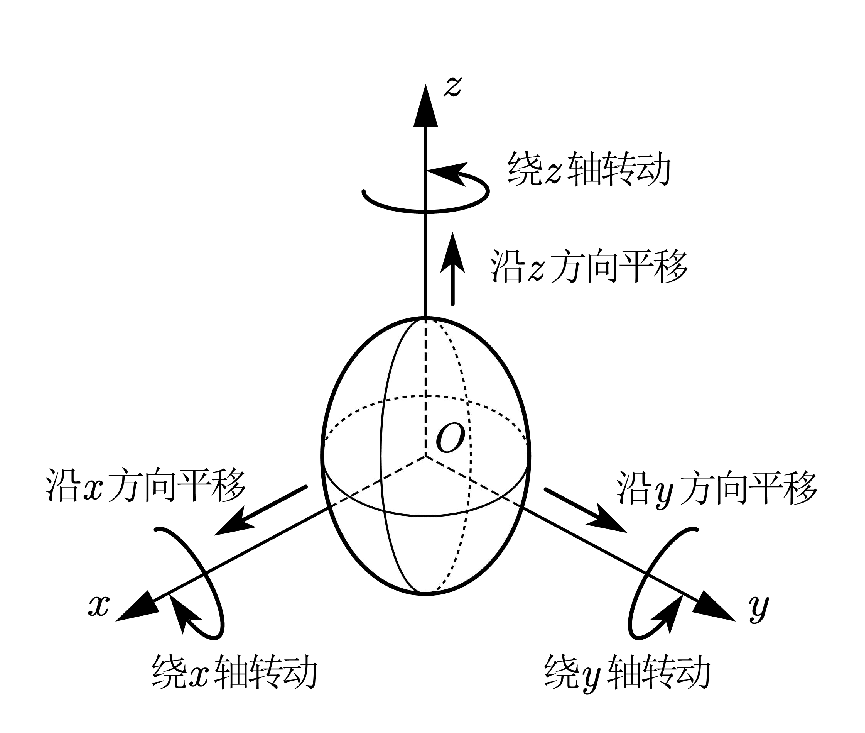
\includegraphics[height = 0.7\linewidth]{freedom.pdf}
    \end{subfigure}\quad
    \begin{subfigure}[t]{0.4\textwidth} \centering
        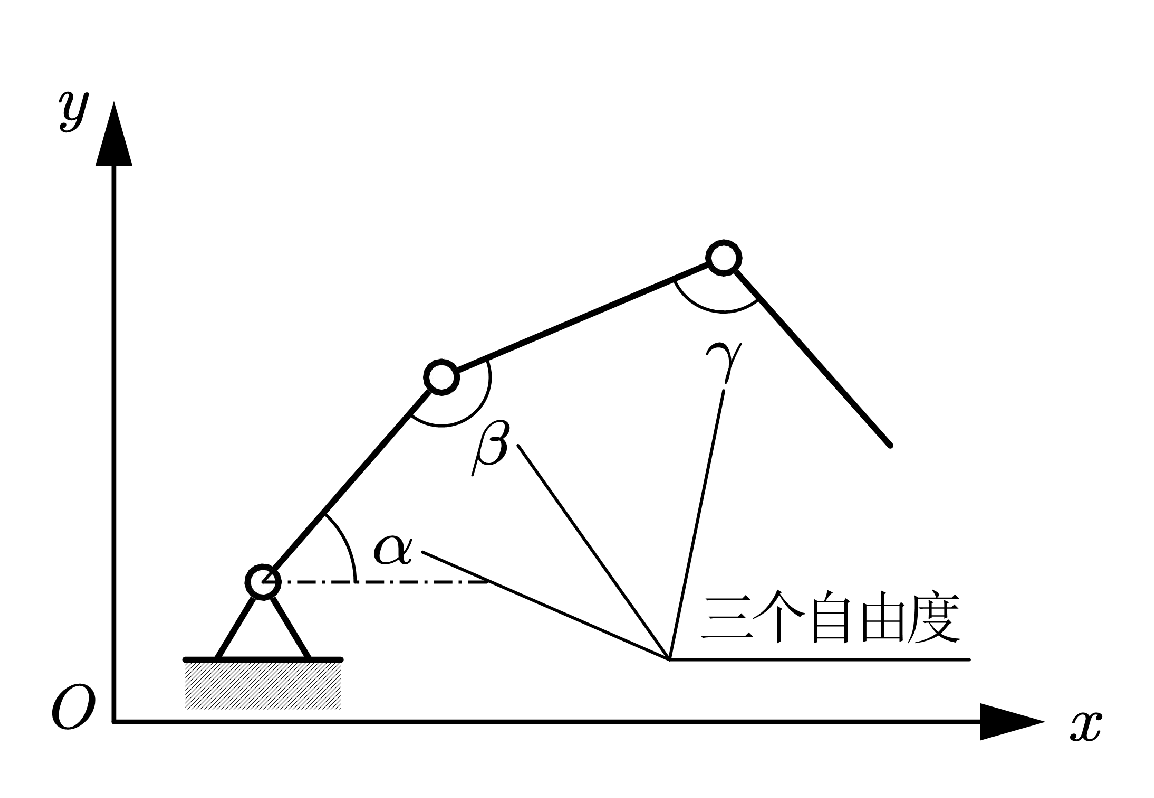
\includegraphics[height = 0.7\linewidth]{machine.pdf}
    \end{subfigure}
    \caption{自由度与约束}
\end{figure}

\uwave{拉格朗日}实现了欧拉的猜想。如果说牛顿力学体系的核心概念是“力”,那么拉格朗日力学体系的核心概念就是“能量”。拉格朗日从牛顿力学出发,结合达朗贝尔原理和虚功原理,推出了\textbf{(第二类)拉格朗日方程}:

\[
    \frac{\mathrm{d}}{\mathrm{d}t}\frac{\partial L}{\partial \dot{q}_i}=0 \quad (i=1,2,\cdots,n)
    .\]

拉格朗日用\textbf{广义坐标}$q_i$来描述物体的空间位置,其中$n$即为自由度数,这时其对时间的导数——广义速度$\dot{q}_i=\dfrac{\mathrm{d} q_i}{\mathrm{d} t}$的概念就不那么直观了。不过,结合坐标和广义坐标之间的关系

\begin{marginparfigure}
    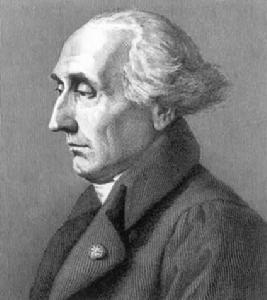
\includegraphics[width = 2.8cm]{Lagrange.jpeg}
    \captionof{figure}{拉格朗日像}
\end{marginparfigure}

\[
    x_j=x_j\left(q_1, q_2, \cdots, q_n\right) \quad \left(j=1, 2, \cdots, N\right)
    .\]

以及偏导数的链式法则,表示出牛顿体系中的物理量还是不困难的。式中的

\[
    L=L(q_1,q_2,\cdots,q_n,\dot{q}_1,\dot{q}_2,\cdots,\dot{q}_n,t)
    .\]

是系统动能与势能之差,我们称之为\textbf{拉格朗日量}。

拉格朗日方程与牛顿的动量定理是等价的,就是说,以二者当中某一个为假设前提,就能推出另一个。拉格朗日体系的数学基础实际上就是变分原理,称
\[
    S=\int_{t_1}^{t_2}{L\,\mathrm{d}t}
    .\]
为\textbf{作用量},当作用量达到极小值(变分等于$0$),就能得到拉格朗日方程。作用量这一概念可以推广到一般的演化系统,只要令某一个演化系统的作用量达到极小值,就能得到一个描述该系统运动规律的方程,这就是\textbf{最小作用量原理}。
\begin{marginpartext}
        牛顿的动量定理指的就是牛顿第二定律,由于$ma$可以写成$\frac{\mathrm{d}p}{\mathrm{d}t}$,其中$p$为动量,这就是动量定理的微分形式,所以有时不区分牛顿第二定律和动量定理。
\end{marginpartext}

拉格朗日体系的高明之处在于回避掉了对复杂约束的讨论,使得问题求解得到简化。然而,拉格朗日体系的好处远不止于此,它虽然是一个和牛顿力学等价的力学体系,但等价不意味着二者完全相等,在分析某些问题时,可能二者当中的某一个更有优势。同时,拉格朗日体系具有更好的泛用性,可以应用在不限于力学的更广泛的问题当中。

\uwave{哈密顿}早期的工作是研究光学,但他将其中的数学方法推广到了力学上,创立了哈密顿力学体系。哈密顿对拉格朗日量$L$进行了勒让德变换
\[
    H\left(q_1,\cdots,q_n,p_1,\cdots,p_n,t\right)=\sum_{i=1}^n{\dot{q}_ip_i}-L\left( q_1,\cdots ,q_n,\dot{q}_1,\cdots ,\dot{q}_n,t \right)
    .\]
其中$p_i$为广义动量。再对该式取变分,就能推出\textbf{哈密顿方程}

\[
    \begin{dcases}
        \dot{q}_i=\dfrac{\partial H}{\partial p_i},  \\
        \dot{p}_i=-\dfrac{\partial H}{\partial q_i}, \\
    \end{dcases} \quad \left( i=1,2,\cdots ,n \right)
    .\]

\begin{marginparfigure}
    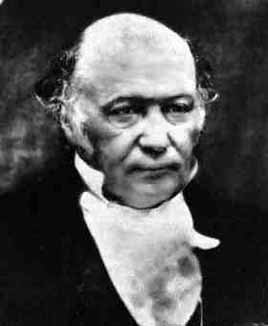
\includegraphics[width = 2.8cm]{Hamilton.jpg}
    \captionof{figure}{哈密顿像}
\end{marginparfigure}

哈密顿推出的方程与拉格朗日的方程和牛顿的运动定律互相等价,但是由于哈密顿的方程具有某种对称性,对于某一类问题的研究和求解来说是很方便的,如量子力学的描述就是基于哈密顿体系的。

这段时期,研究人员注意到所谓守恒律实际上是运动方程的某种积分。\uwave{索菲斯·李}对微分方程进行研究,将微分方程的解与变换群相联系,这使得对微分方程解的研究也可以用到近世代数的手段。\uwave{诺特}进一步提出,作用量的连续对称性意味着守恒。这些思想在日后的物理学研究中发挥着重要的作用。

\subsubsection{力学进一步发展的时代——连续介质力学}

对连续介质力学的研究分为固体力学和流体力学两部分,起初这二者之间没有建立联系,随着研究的逐渐深入,才将它们纳入到一个统一的框架下进行描述。

\begin{marginpartext}
        气体中的激波是这样形成的:气体中扰动产生的波以当地声速进行传播,当扰动源的运动速度超过当地声速时,扰动来不及传播到扰动源前边,这样产生了一个压缩界面,这就是激波。超音速飞行器产生的爆鸣声就是激波导致压强突变产生的。
\end{marginpartext}

对流体的研究比固体的稍早。牛顿在《自然哲学的数学原理》之中,就对流体进行了讨论,提出了“牛顿流体”的概念。之后,\uwave{丹尼尔·伯努利}、欧拉等人建立了不考虑流体粘性的理想流体的动力学方程,但真实流体存在粘性,所以这部分理论只有在粘性可以忽略时才能实用。不过,理想流体动力学的观点和方法论对后序研究是很有价值的。

\uwave{纳维}考虑了流体的粘性,推导出了不可压缩粘性流体的运动方程,稍后,也从连续介质假设出发推导出了这组方程,这就是著名的\textbf{纳维-斯托克斯方程}(N-S方程):

\[
    \frac{\partial(\rho\symbfit{u})}{\partial t}+\nabla\cdot(\rho\symbfit{uu})=\rho\symbfit{f}-\nabla p+\mu\nabla ^2\symbfit{u}
    .\]

在直角坐标系中,将每一项展开就可以写成:
\[
    \begin{dcases}
        \dfrac{\partial v_x}{\partial t}+v_x\dfrac{\partial v_x}{\partial x}+v_y\dfrac{\partial v_x}{\partial y}+v_z\dfrac{\partial v_x}{\partial z}=f_x-\dfrac{1}{\rho}\dfrac{\partial p}{\partial x}+\nu\left(\dfrac{\partial^2 v_x}{\partial x^2}+\dfrac{\partial^2 v_x}{\partial y^2}+\dfrac{\partial^2 v_x}{\partial z^2}\right), \\
        \dfrac{\partial v_y}{\partial t}+v_x\dfrac{\partial v_y}{\partial x}+v_y\dfrac{\partial v_y}{\partial y}+v_z\dfrac{\partial v_y}{\partial z}=f_y-\dfrac{1}{\rho}\dfrac{\partial p}{\partial y}+\nu\left(\dfrac{\partial^2 v_y}{\partial x^2}+\dfrac{\partial^2 v_y}{\partial y^2}+\dfrac{\partial^2 v_y}{\partial z^2}\right), \\
        \dfrac{\partial v_z}{\partial t}+v_x\dfrac{\partial v_z}{\partial x}+v_y\dfrac{\partial v_z}{\partial y}+v_z\dfrac{\partial v_z}{\partial z}=f_z-\dfrac{1}{\rho}\dfrac{\partial p}{\partial z}+\nu\left(\dfrac{\partial^2 v_z}{\partial x^2}+\dfrac{\partial^2 v_z}{\partial y^2}+\dfrac{\partial^2 v_z}{\partial z^2}\right).
    \end{dcases}
\]
这组方程的求解十分困难,以至于时至今日,该组方程光滑解的存在性还没有得到证明。

不可压缩流体的典型便是水,这段时期,得益于不可压缩流体的研究成果日益丰富,水力学和水动力学也得到了发展。许多水利工程、水力机械结合生产经验以及理论分析,获得了许多经验和半经验的公式,大大促进了工程学的发展。

20世纪之前,对于可压缩流体的研究则比较少,主要围绕超声速流动和激波展开,做了基础性的探索。

最早的固体力学来自于对杆、梁、板等变形体的变形、强度、稳定性等问题的研究。早期,伽利略考察过悬臂梁的强度问题;稍晚一些的欧拉考察了梁的小挠度变形(横向变形,即垂直于轴向的变形),以及压杆稳定性问题。

\begin{marginparfigure}
    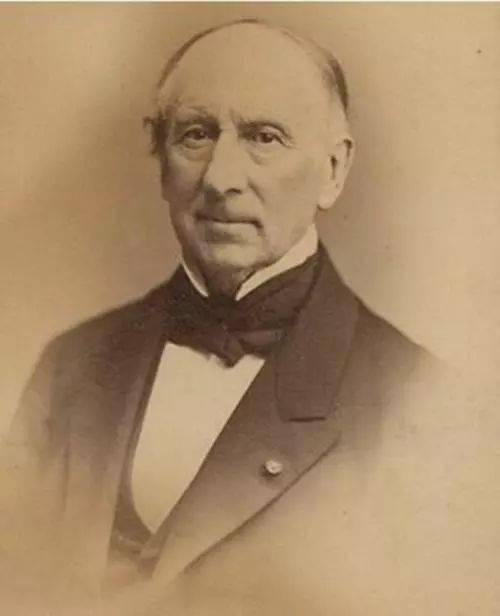
\includegraphics[width = 2.8cm]{Cauchy.jpeg}
    \captionof{figure}{柯西像}
\end{marginparfigure}


随后一段时间,固体力学的研究主要围绕弹性力学展开,这一部分的研究也是比较成熟的。弹性力学理论的先驱是纳维和\uwave{泊松},纳维提出了各向同性弹性体的平衡方程,泊松给出了\textbf{泊松比}的概念。弹性力学理论的奠基者是\uwave{柯西},他引入了\textbf{应变}、\textbf{应力}的概念,讨论了应力应变之间的关系,讨论了平衡微分方程和边界条件的提法,这些内容是线弹性力学的基本内容。

\begin{marginpartext}
        应力描述内力的分布情况,它的量纲与压强相同。

        应变描述变形情况,它的量纲是$1$。

        泊松比描述变形过程中的横向收缩效应。
\end{marginpartext}


\begin{figure}[ht]
    \centering
    \begin{subfigure}[t]{0.8\textwidth} \centering
        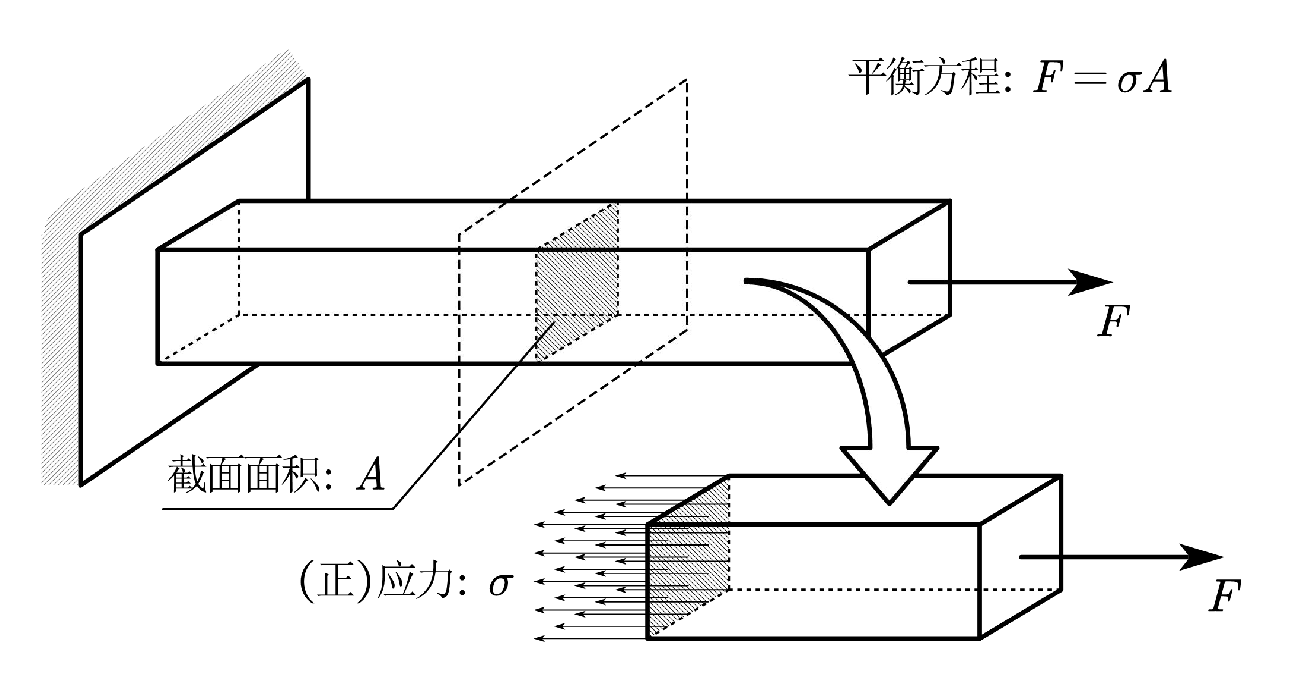
\includegraphics[height = 0.5\linewidth]{stress.pdf}
    \end{subfigure}
    
    \begin{subfigure}[t]{0.8\textwidth} \centering
        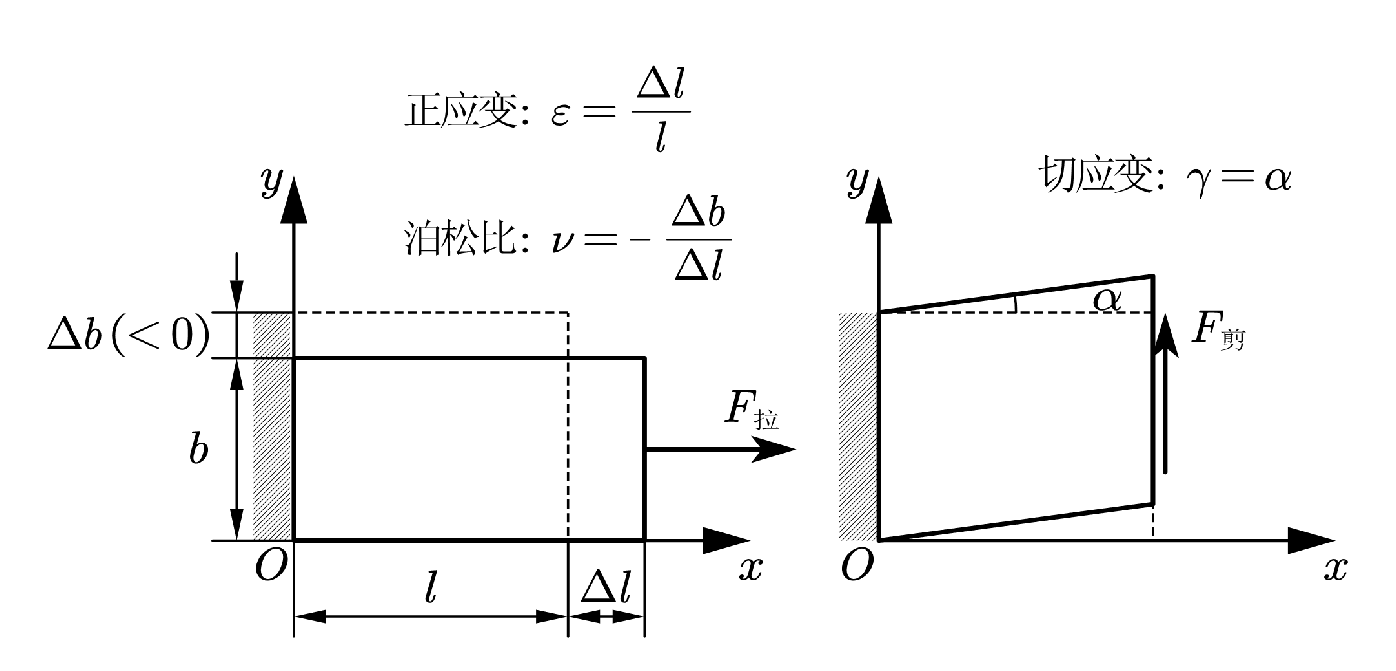
\includegraphics[height = 0.5\linewidth]{strain.pdf}
    \end{subfigure}
    \caption{应力、应变与泊松比}
\end{figure}


\begin{marginparfigure}
    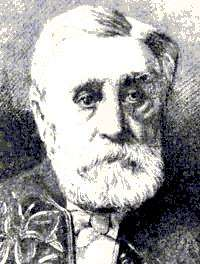
\includegraphics[width = 2.8cm]{Saint_Venant.jpeg}
    \captionof{figure}{圣维南像}
\end{marginparfigure}

建立起弹性力学相关的基本概念后,学者们研究了一些弹性模型的解法。\uwave{圣维南}%
提出了逆解法和半逆解法,是弹性力学求解的重要手段;以及\textbf{圣维南原理},描述了弹性体的局部效应,对于问题求解很有好处。\uwave{柯希霍夫}(基尔霍夫)研究了薄板的理论。\uwave{瑞利}总结了弹性体的振动和声学问题。\uwave{勒夫}总结了前人关于弹性力学的工作,并进一步发展,讨论了薄壳问题,同时还研究了弹性波理论。\uwave{穆斯赫利什维利}致力于用复变函数的手段解析求解弹性力学问题,是计算力学发展之前弹性理论求解的高峰。


\begin{marginpartext}
        复变函数指的是自变量和因变量都是复数的函数,它在描述一些平面问题时具有优势,故在固体力学、流体力学中都有应用。
\end{marginpartext}

\begin{figure}[h]
    \centering
    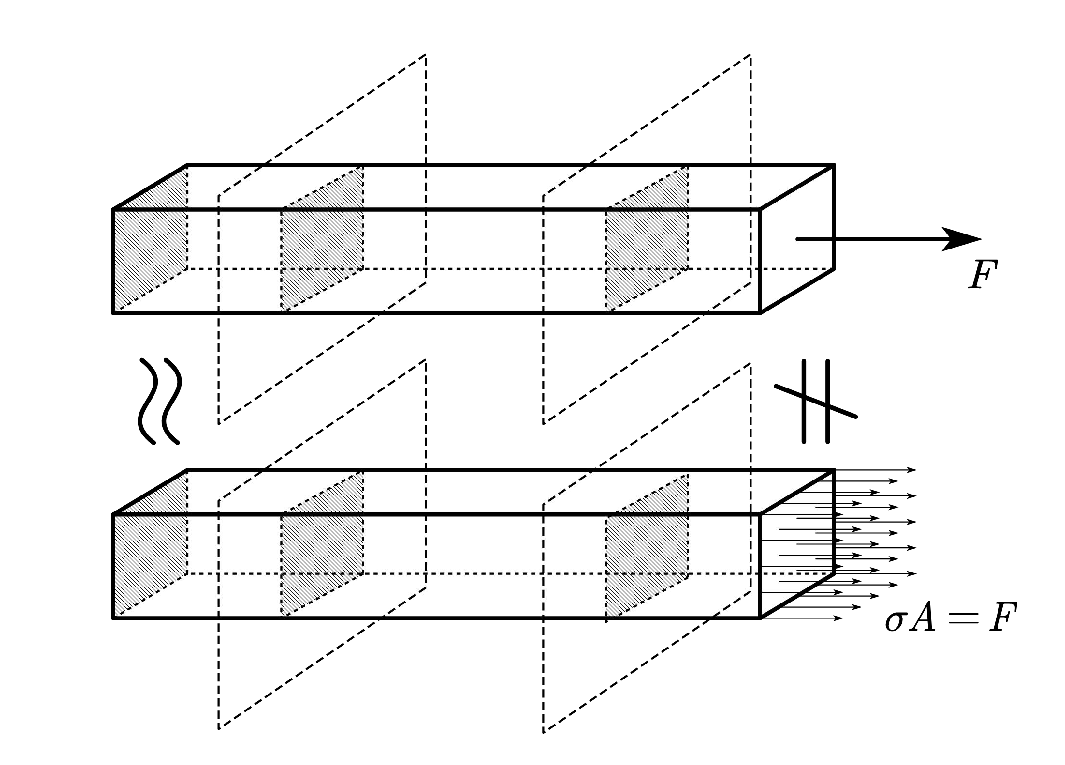
\includegraphics[scale=0.45]{StVenant.pdf}
    \caption{圣维南原理示意}
\end{figure}

弹性力学的发展完善了对\uwave{杆}、\uwave{梁}、\uwave{轴}等基本结构件变形和强度的研究,获得了一些简单且具有工程实用性的结果,这一部分当属材料力学的范畴。同时期,工程上开始结构的变形问题,最典型的是桁架结构和连续梁,并发展了一些求解的方法,这当属结构力学的范畴。此外,由于工程实际的需要和工程事故,人们开始关注疲劳和断裂现象。

\begin{marginpartext}
        一般来说,杆、梁、轴都是细长结构件,区别在于:杆只承受轴向拉压,梁只承受横向外力(弯曲),轴只承受扭转。
\end{marginpartext}

\begin{figure}[ht]
    \centering
    \begin{subfigure}[t]{0.3\textwidth} \centering
        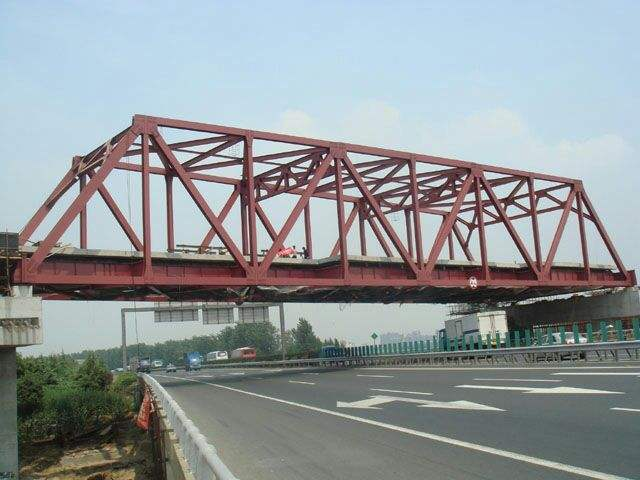
\includegraphics[height = 0.7\linewidth]{truss.jpeg}
        \caption{桁架结构}
    \end{subfigure}\quad
    \begin{subfigure}[t]{0.6\textwidth} \centering
        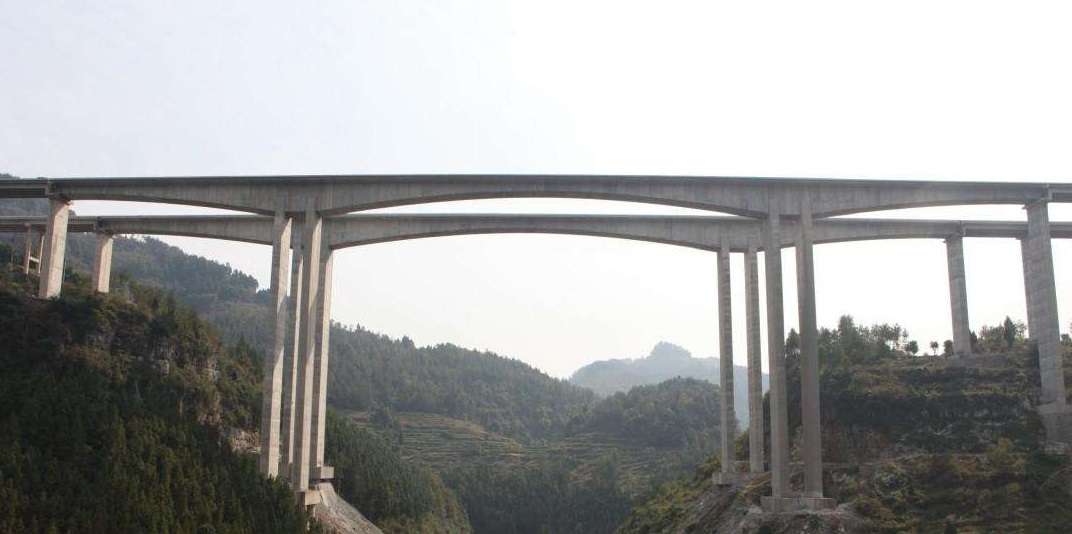
\includegraphics[height = 0.35\linewidth]{continuous_beam.jpeg}
        \caption{连续梁结构}
    \end{subfigure}\bigskip

    \begin{subfigure}[t]{0.8\textwidth} \centering
        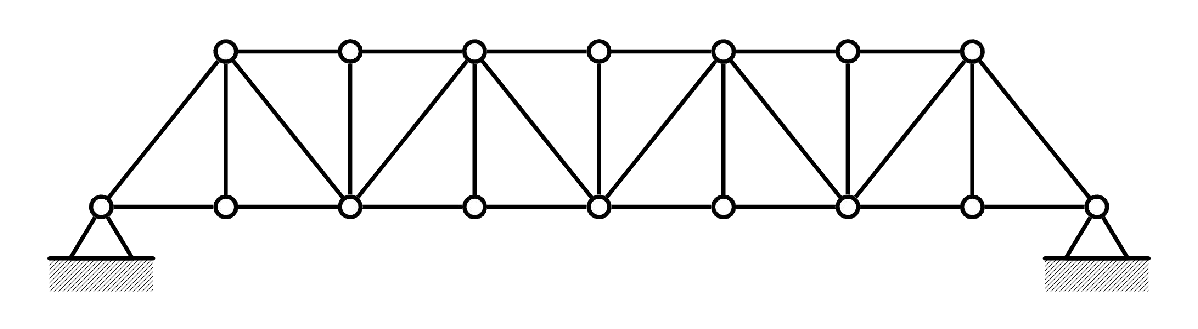
\includegraphics[width = 0.75\textwidth]{truss_model.pdf}
        \caption{桁架模型}
    \end{subfigure}\bigskip

    \begin{subfigure}[t]{0.6\textwidth} \centering
        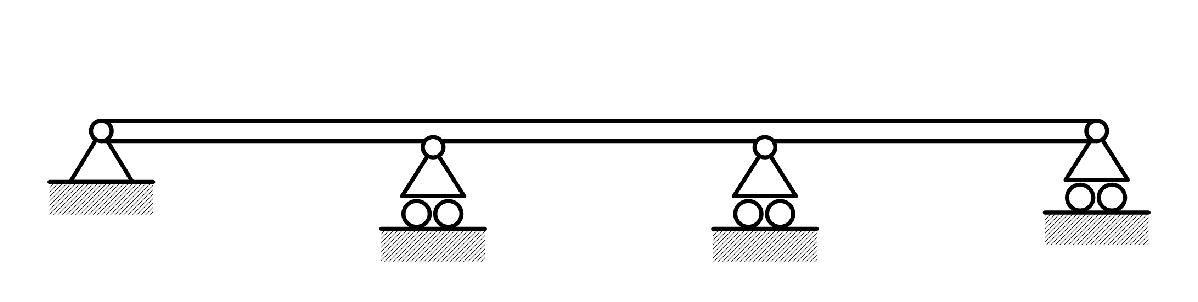
\includegraphics[width = \textwidth]{beam_model.pdf}
        \caption{连续梁模型}
    \end{subfigure}
    \caption{典型工程结构及其模型}
\end{figure}

\subsubsection{近代力学}

20世纪初,经典物理学面临着两大问题,其一是黑体辐射问题,由此产生了量子力学,其二是探讨光速不变的问题,由此产生了相对论。从此开始,物理学和力学之间出现了比较明显的界限。

\begin{figure}[ht]
    \centering
    \begin{subfigure}[t]{0.45\textwidth} \centering
        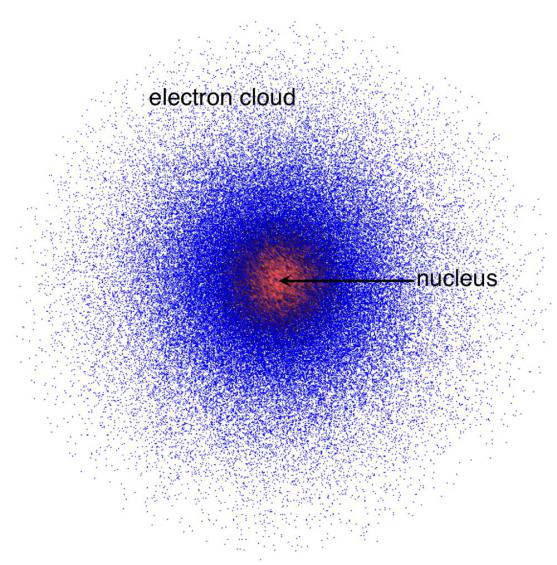
\includegraphics[height = 0.55\linewidth]{quantum.png}
        \caption{量子力学中的电子云图}
    \end{subfigure}\quad
    \begin{subfigure}[t]{0.45\textwidth} \centering
        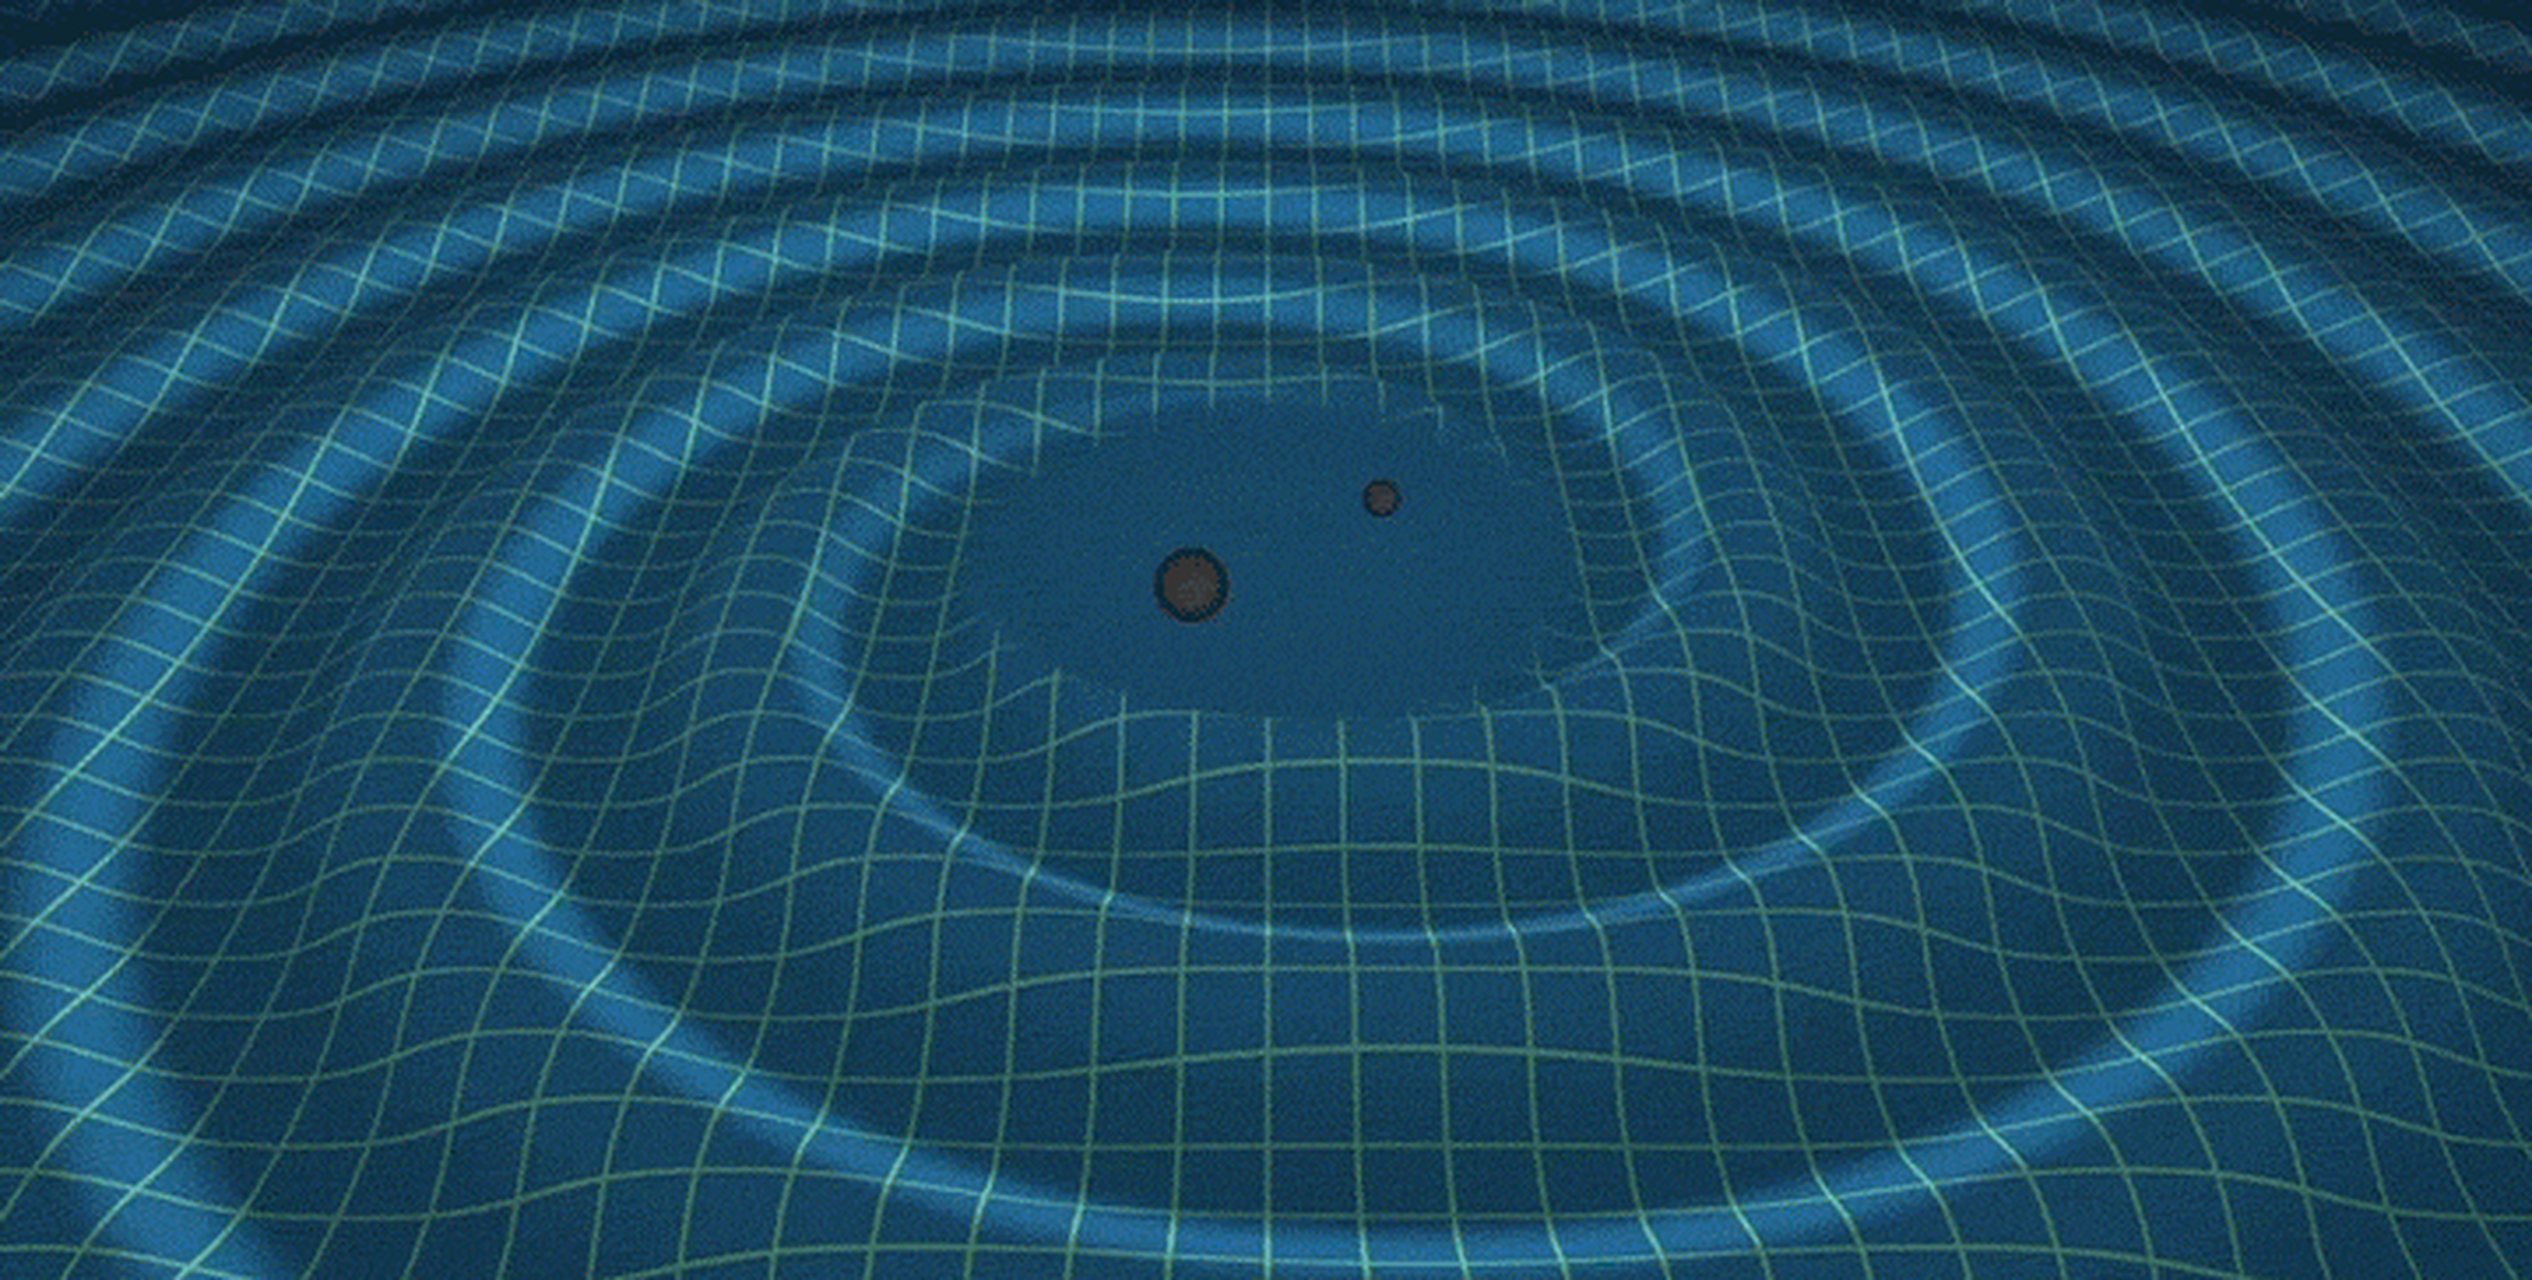
\includegraphics[height = 0.55\linewidth]{relativity.jpeg}
        \caption{广义相对论所预言的引力波现象}
    \end{subfigure}
\end{figure}

量子力学关心原子、分子尺度上基本粒子的性质,相对论则深入地考虑了我们所处宇宙的时空背景。这二者都是在不同情况下对经典力学的修正,经过适当的退化,它们可以分别得到经典力学中的结果。同时,经典力学能够足够精确地描述宏观、低速下的物理问题,而且这些问题还没有被完全解决,所以经典力学不仅没有走到尽头,反而得到进一步的发展,直至今天,形成了目前的力学这一学科。

时间来到20世纪,力学比较明显地分化出了“应用派”和“理论派”。这是由于,一方面理论物理的发展已经远远超过工程实践的能力,于是诸多工程内容需要依靠力学理论指导进行;另一方面,即使是经典力学中尚有诸多问题没有得到回答,有些知识更需要建立一个完善的体系。这种分化也不是20世纪才出现的,事实上早已有之,总有一些理论是比较超前的,暂时找不到它的用处,也有一些理论是为了解决当前的问题而提出的半经验或经验的模型,这就分别对应“理论派”和“工程派”。不过,这二者之间不是完全对立的关系,理论与实践是相辅相成的,只是二者之间分化的趋势到20世纪比以前更加明显了。目前,将力学与工程相结合是主要的趋势。

20世纪初这段时间的力学发展了以下主要内容:

一般力学中的许多问题最终都归结到求解常微分方程组中,不过解析求解一般的常微分方程组是困难的,于是人们便去研究方程的性质和行为。在研究非线性微分方程的过程中,陆续发现了周期解、非线性振动、分叉、混沌等现象,促进了微分方程定性理论的发展。

\begin{figure}[ht]
    \centering
    \begin{subfigure}[t]{0.45\textwidth} \centering
        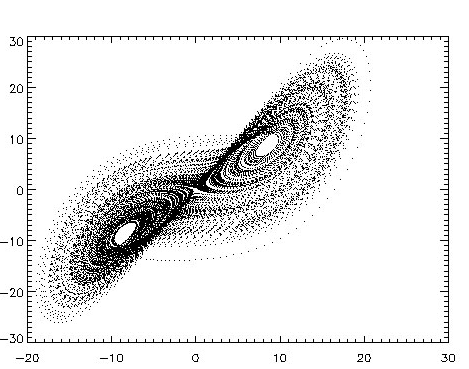
\includegraphics[height = 0.55\linewidth]{chao.jpeg}
        \caption{混沌现象中的奇异吸引子}
    \end{subfigure}\quad
    \begin{subfigure}[t]{0.45\textwidth} \centering
        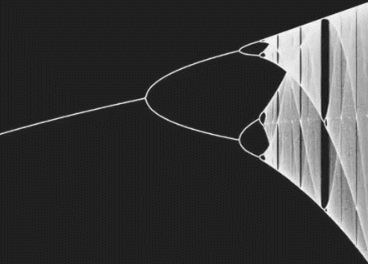
\includegraphics[height = 0.55\linewidth]{bifurcation.png}
        \caption{分叉现象}
    \end{subfigure}\bigskip

    \begin{subfigure}[t]{0.45\textwidth} \centering
        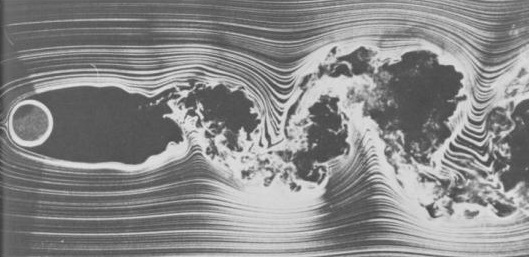
\includegraphics[height = 0.55\linewidth]{turbulent.jpeg}
        \caption{圆柱绕流产生的湍流现象}
    \end{subfigure}
\end{figure}


流体力学部分继续对N-S方程进行研究。N-S方程具有强烈的非线性,它具有描述湍流现象的能力,但求解是十分困难的。雷诺将速度写为平均速度与脉动速度之和,将压强写为平均压强与脉动压强之和,得到了平均意义下的N-S方程,后人称之为雷诺方程。\uwave{普朗特}、\uwave{冯·卡门}、\uwave{泰勒}、\uwave{周培源}、\uwave{柯尔莫哥洛夫}进一步做了一些工作,开创了湍流统计理论的研究。另一边,飞机的发明刺激了对机翼升力问题的研究,普朗特、\uwave{兰开斯特}、\uwave{芒克}等人合作建立了“升力线”理论,对翼型设计起到了指导作用。

\begin{marginparfigure}
    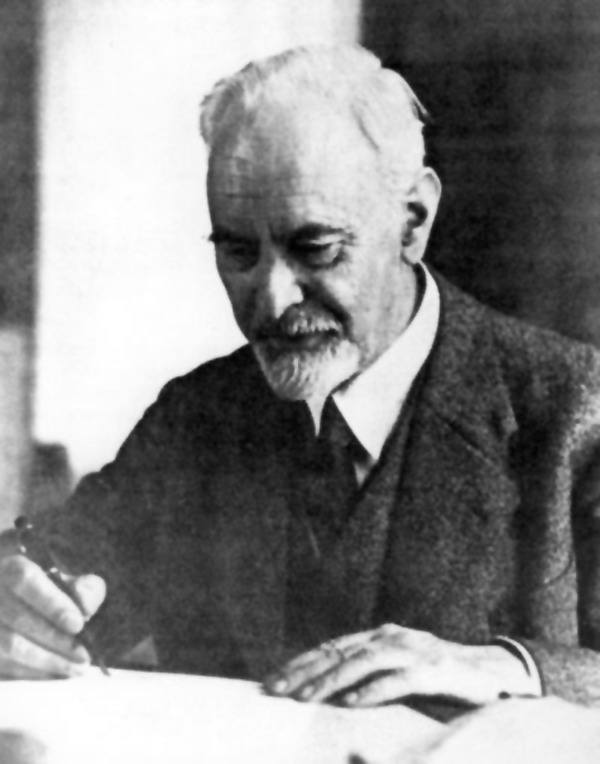
\includegraphics[width = 2.8cm]{Prandtl.jpeg}
    \captionof{figure}{普朗特像}
\end{marginparfigure}


\begin{marginparfigure}
    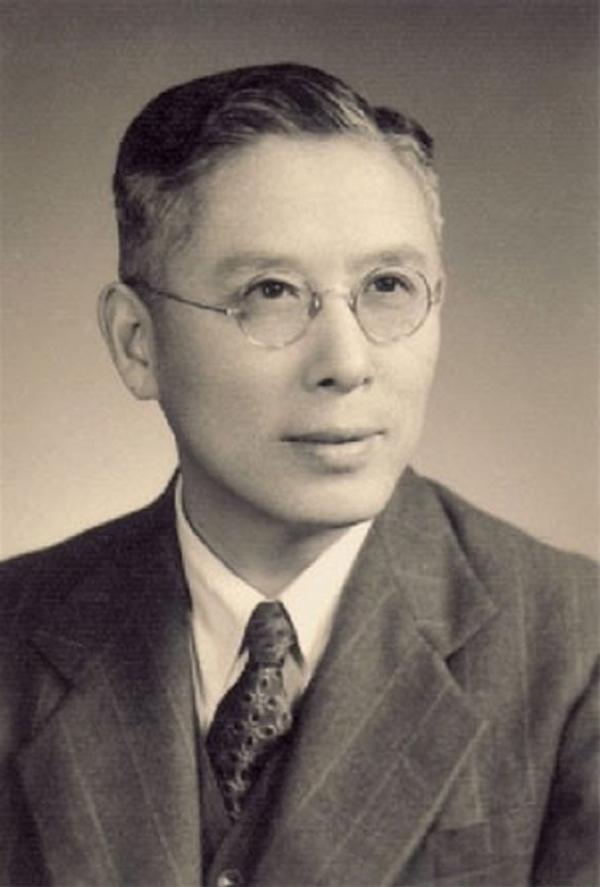
\includegraphics[width = 2.8cm]{Zhou.jpeg}
    \captionof{figure}{周培源像}
\end{marginparfigure}



\begin{figwindow}[0,r,
        {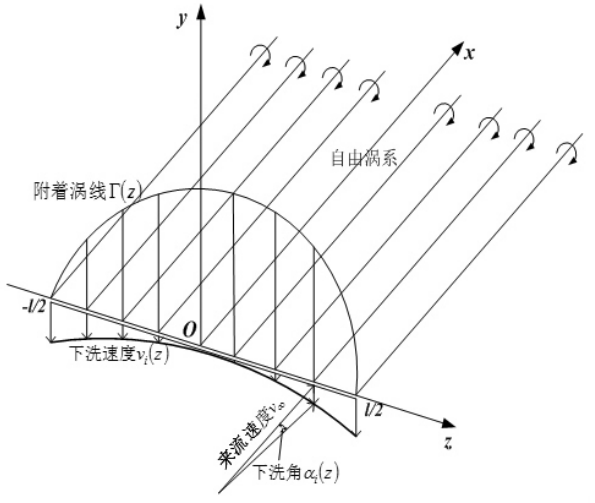
\includegraphics[width = 0.4\linewidth]{liftingline.png}},
        升力线模型]
    固体力学部分,人们已经将弹性理论中的大部分线性问题研究清楚了,这时开始考虑梁、板、壳等结构的稳定性,以及板壳的一般理论等。塑性力学、断裂力学以及疲劳问题等研究也已开始进行,就是说,这段时间的研究以及不再限于线弹性问题,而是向更多的非线性问题发起冲击。此外,麦克斯韦等考虑了黏弹性体模型,进而引发了人们对一般连续介质的性质的探讨,并最终形成了连续介质力学,并且促进了理性力学的复兴。
\end{figwindow}



此外值得一提的是计算机的发明导致了计算力学这一分支的产生。20世纪初,人们已经需要求解大规模复杂工程中的力学问题,但庞大的问题规模时代靠人力解决这些问题是极端困难的。计算机的问世和发展,强化了人类的计算能力,使得求解大规模力学问题成为可能。计算力学就是这样一门借助计算机解决力学问题、分析力学性质的学科,它处于力学、数学、计算机三门学科交叉的位置。计算力学当中的方法已经能够比较好地解决大部分线性问题,而对于数学本质是非线性的问题,如何用计算力学的手段去解决和分析还是很有挑战性的课题。

\begin{figure}
    \centering
    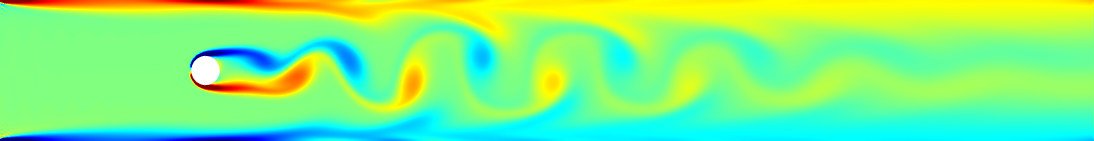
\includegraphics[width = \textwidth]{calculation_fluent.png}
    \caption{基于MATLAB编写的圆柱绕流涡量图计算结果}
\end{figure}

\begin{figure}
    \centering
    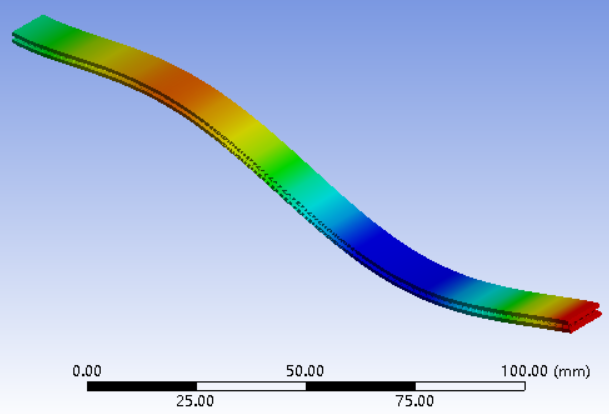
\includegraphics[scale=0.7]{calculation_solid.png}
    \caption{基于商业有限元软件ANSYS Workbench的悬臂梁自由振动位移云图}
\end{figure}

\subsection{力学的研究内容}

概括地说,力学是\textbf{研究宏观低速的物体机械运动规律的学问}。这一句话中包含了两个限定以及研究的对象。

\textbf{宏观},指的是忽略量子效应,而不一定是肉眼可见才叫宏观,有时,力学也会研究微纳米尺寸的问题,而不计量子效应的影响。\textbf{低速},指的是忽略相对论效应,天体力学能够解决太阳系范围内很多天体运动的问题,但在更大尺度的宇宙环境中,可能要考虑相对论效应的影响,这已经超出力学的研究范畴。总之,除了个别的极特殊情况,我们所讨论的力学都是经典范畴的。

\textbf{物体},其含义可以按照基于某种假设将实际物体抽象成的某种模型,再对这个模型加以研究。这些模型无外乎以下几种:\uwave{质点}、\uwave{刚体}、\uwave{连续介质}。

我们在中学阶段就学过了质点模型,这种模型假设忽略物体的尺寸大小,将物体视为有质量的点,例如,在考虑行星绕恒星运动时就会应用质点模型。

刚体则考虑了物体的尺寸、形状,但仍然认为物体是刚度无穷大的,也就是不会发生变形,准确的说法是“在物体上任取两点,这两点的距离是一个恒定值”。这种刚体模型相较于质点模型更加常见,杆、齿轮等机械构件在运动时,不可以忽略其形状因素,这时可以将它们视为刚体。

\begin{figwindow}[2,l,{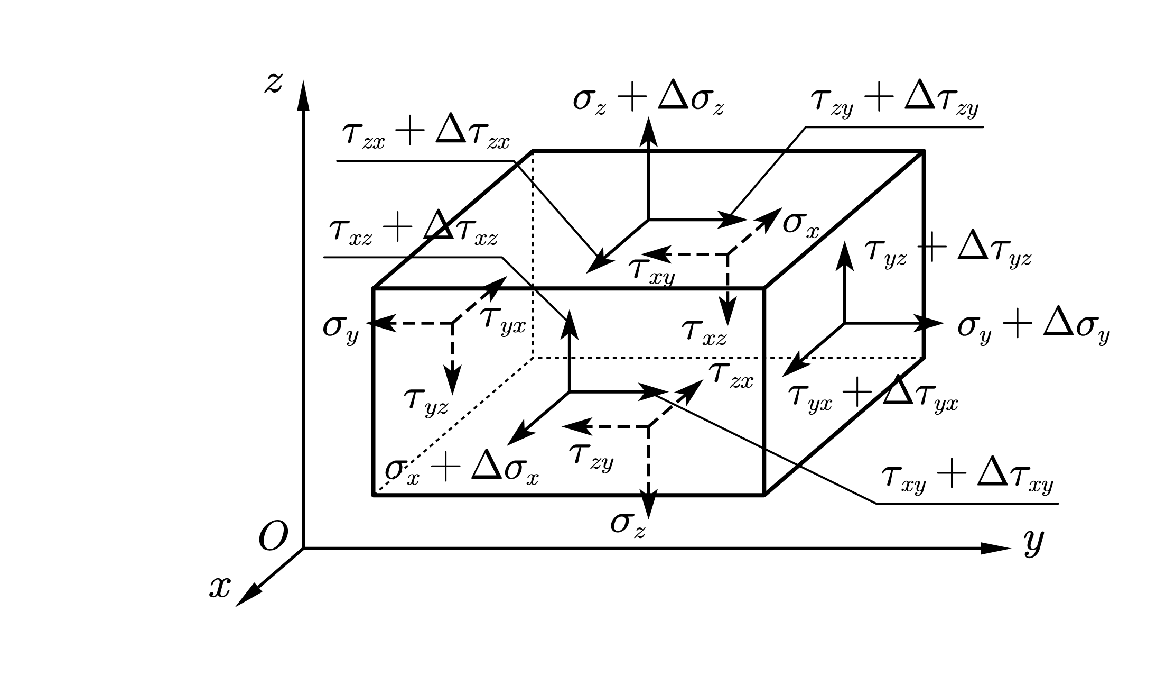
\includegraphics[width = 0.6\linewidth]{infinitesimal.pdf}},
        线弹性变形体微元的受力分析]
    连续介质是一个相当宽泛的模型,它可以涵盖多数固体、液体、气体。其最显著的特征是要考虑物体的变形。我们将etcounter这种模型称为“连续介质”的原因是,该模型的基本假设是“连续性假设”,即材质相同的一块物质是无限可分的,这样就可以应用微积分、场论等分析学工具对物体的变形加以研究。再根据物体变形的性质(可以理解为内力与变形及变形速率的关系)不同对其进行分类,粗略地讲,按照物体能否有效地抵抗剪切力将物体分为固体和流体,再按照流体是否可发生压缩变形分为气体和液体,按不同类别分别加以研究。例如,在研究杆、梁、轴的变形时,将它们视为固体;水是典型的液体,空气是典型的气体。
\end{figwindow}



\textbf{机械运动}是描述物体的空间位置随时间变化的过程,大致可分为\uwave{刚性运动}和\uwave{变形}。所谓刚性运动,即是指质点和刚体可以发生的机械运动,如平移、转动;而变形是物体的形状在外界作用下发生了变化,如弹簧的形变、弹性体的形变等。

我们首先对力学的研究范围做了一个大致限定,也了解了力学中的一些基本模型和概念。然而在某些必要的时候,可以适当放宽这些限制,力学的研究对象也可能随着科学技术的进一步发展而得到扩充。
目前,力学学科的二级分类大致就按照模型不同,分为\textbf{一般力学(与力学基础)}、\textbf{固体力学}和\textbf{流体力学},此外还有更加面向工程应用的\textbf{工程力学}和一些其他分支。下面,我们具体到目前力学学科的主要分支当中,看看不同力学分支的主要研究内容。

\subsubsection{一般力学与力学基础}

一般力学大致是动力学与控制的同义词,它的研究对象是宏观的离散力学系统和经典力学的一般原理。力学基础的对象比较广泛,但仍以离散系统为主。

\paragraph{天体力学}

天体力学是天文学和力学之间的交叉学科,研究对象小至太阳系内的天体,大至恒星系。其又下含几个次级学科,包括摄动理论、定性分析、数值计算、天体形状与自旋理论等,以及其他一些相对独立的课题。

\begin{figure}[ht]
    \centering
    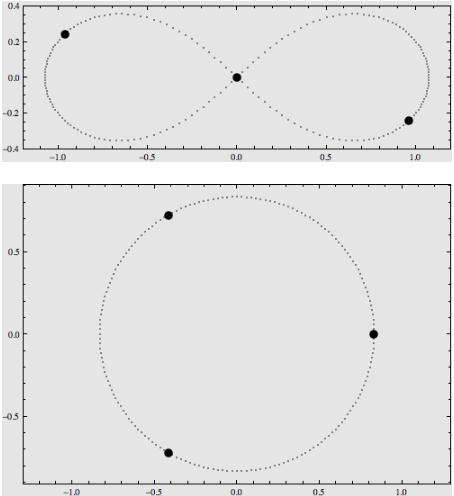
\includegraphics[scale=0.6]{three_bodies.jpeg}
    \caption{天体力学中的三体问题,两个特殊解}
\end{figure}

\paragraph{刚体动力学}

刚体动力学研究刚体在外力作用下的运动规律。它是计算机器部件的运动,舰船、飞机、火箭等航行器的运动以及天体姿态运动的力学基础。主要的次级研究内容有陀螺力学、转子动力学等。


\paragraph{分析力学}

分析力学通过用广义坐标为描述质点系的变量,运用数学分析的方法,研究宏观现
象中的力学问题。早期内容包括拉格朗日力学和哈密顿力学,后来又对有约束系统做了讨论。目前理论体系已经比较完备,主要考虑其具体应用。

\paragraph{运动稳定性}

运动稳定性研究物体或系统在外干扰的作用下偏离其原有运动后返回该运动的性质,对于运动稳定性的研究大都出于工程技术需要。奠定运动稳定性相关理论基础的是\uwave{庞加莱}和\uwave{李雅普诺夫}%
\begin{marginparfigure}
    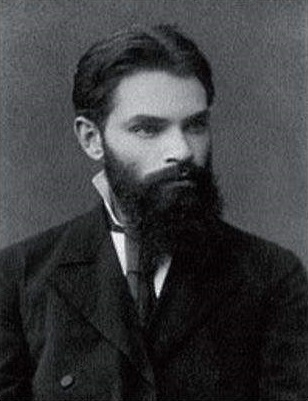
\includegraphics[width = 2.8cm]{Lyapunov.jpeg}
    \captionof{figure}{李雅普诺夫像}
\end{marginparfigure}%
,特别是李雅普诺夫开创的分析方法已经在诸多领域中得到应用。

\paragraph{非线性振动}

恢复力与位移不成正比或阻尼力不与速度一次方成正比的系统的振动都算是非线性振动。线性振动理论已经发展得比较完善,但在实际问题中,总有一些用线性理论无法解释的现象。一般来说,线性模型只适用于小运动范围,超出这一范围,按线性问题处理就会引起较大误差。

\begin{figure}
    \centering
    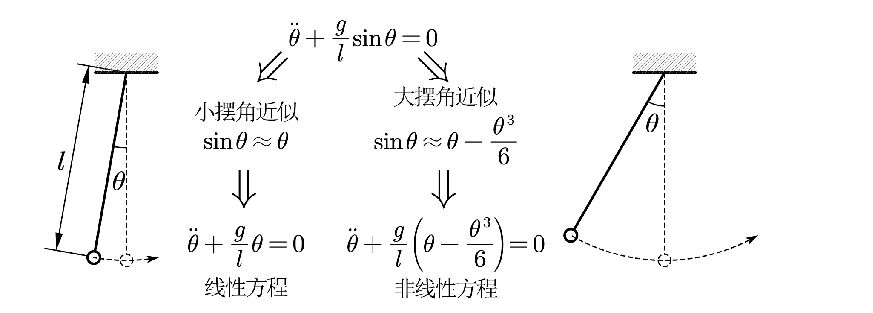
\includegraphics[width = 13cm]{pendulum.pdf}
    \caption{最简单的非线性振动的例子:大摆角单摆振动}
\end{figure}


\subsubsection{固体力学}

固体力学是力学当中成形较早、理论性和应用性都比较强的一个分支。它主要研究变形体在外界影响下内部发生的运动、变形等规律。固体力学当中的线弹性、小变形理论已经发展得相当完善,目前研究的方向多是非线性问题及随机性问题,典型的非线性问题有大变形、稳定性、断裂、疲劳、冲击等。


\begin{wrapfigure}[9]{r}{5cm}
    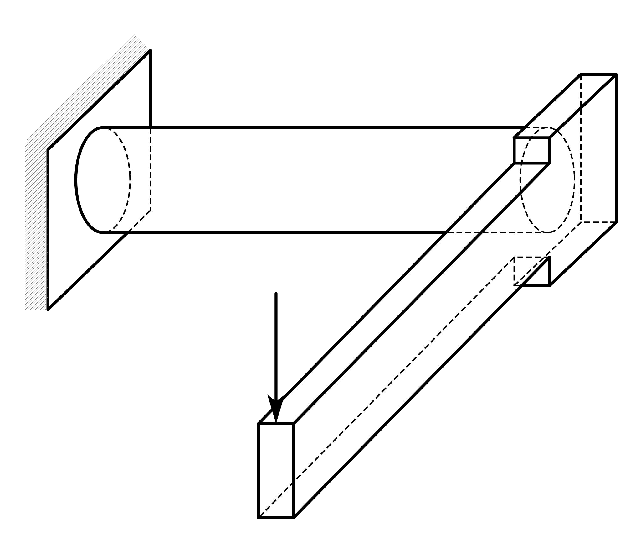
\includegraphics[width=5cm]{material_mechanics.pdf}
    \caption{材料力学中一个承受弯扭作用的结构件}
\end{wrapfigure}
\paragraph{材料力学} 材料力学主要研究简单结构件的变形、稳定性和强度问题。广泛地说,断裂、疲劳、强度、蠕变、试验测定等都可归入到材料力学的范畴。实际上,材料力学并不能算是一个独立的研究方向,它其实是在弹性力学获得结果的基础上,引入合理的假设,得到足够工程实用的结果。因此,材料力学更像是面向工程师的弹性力学简化版,或者作为入门固体力学时的学习材料。


\paragraph{结构力学}



结构力学研究的是杆、梁、\uwave{板}、\uwave{壳}等工程基本结构及其组合的变形和受力。结构力学由材料力学和弹性力学发展而来,主要研究内容有结构静力学、结构动力学、稳定性理论、断裂和疲劳。其中,结构静力学的发展比较成熟,并且由其中的“位移法”产生了计算力学的雏形。结构动力学研究的是在动态外载作用下结构的响应,主要围绕结构振动展开。稳定性理论、断裂和疲劳则是关注工程结构,而非一般的弹性体。

\begin{figure}[h]
    \centering
    \begin{subfigure}[t]{0.4\textwidth} \centering
        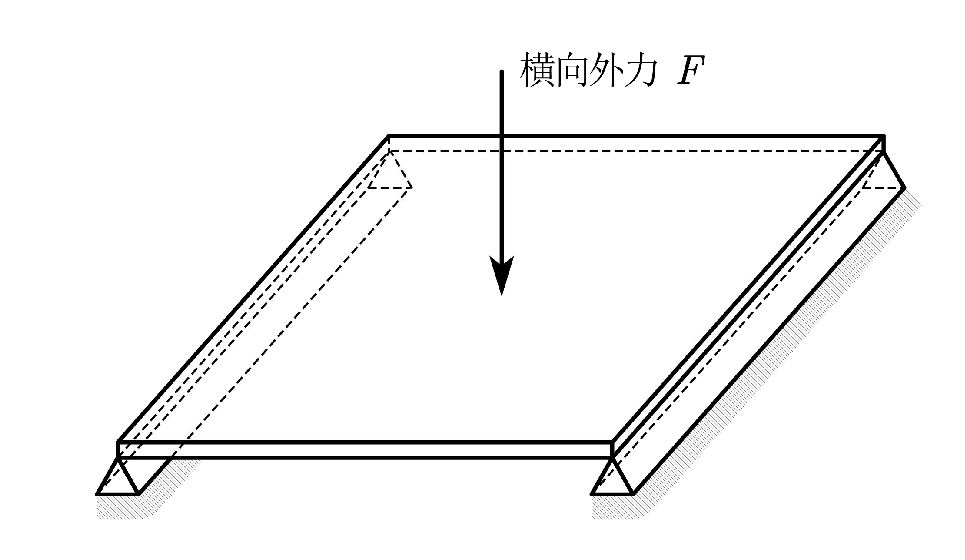
\includegraphics[height = 0.55\linewidth]{plate.pdf}
        \caption{两边简支薄板}
    \end{subfigure}\quad
    \begin{subfigure}[t]{0.4\textwidth} \centering
        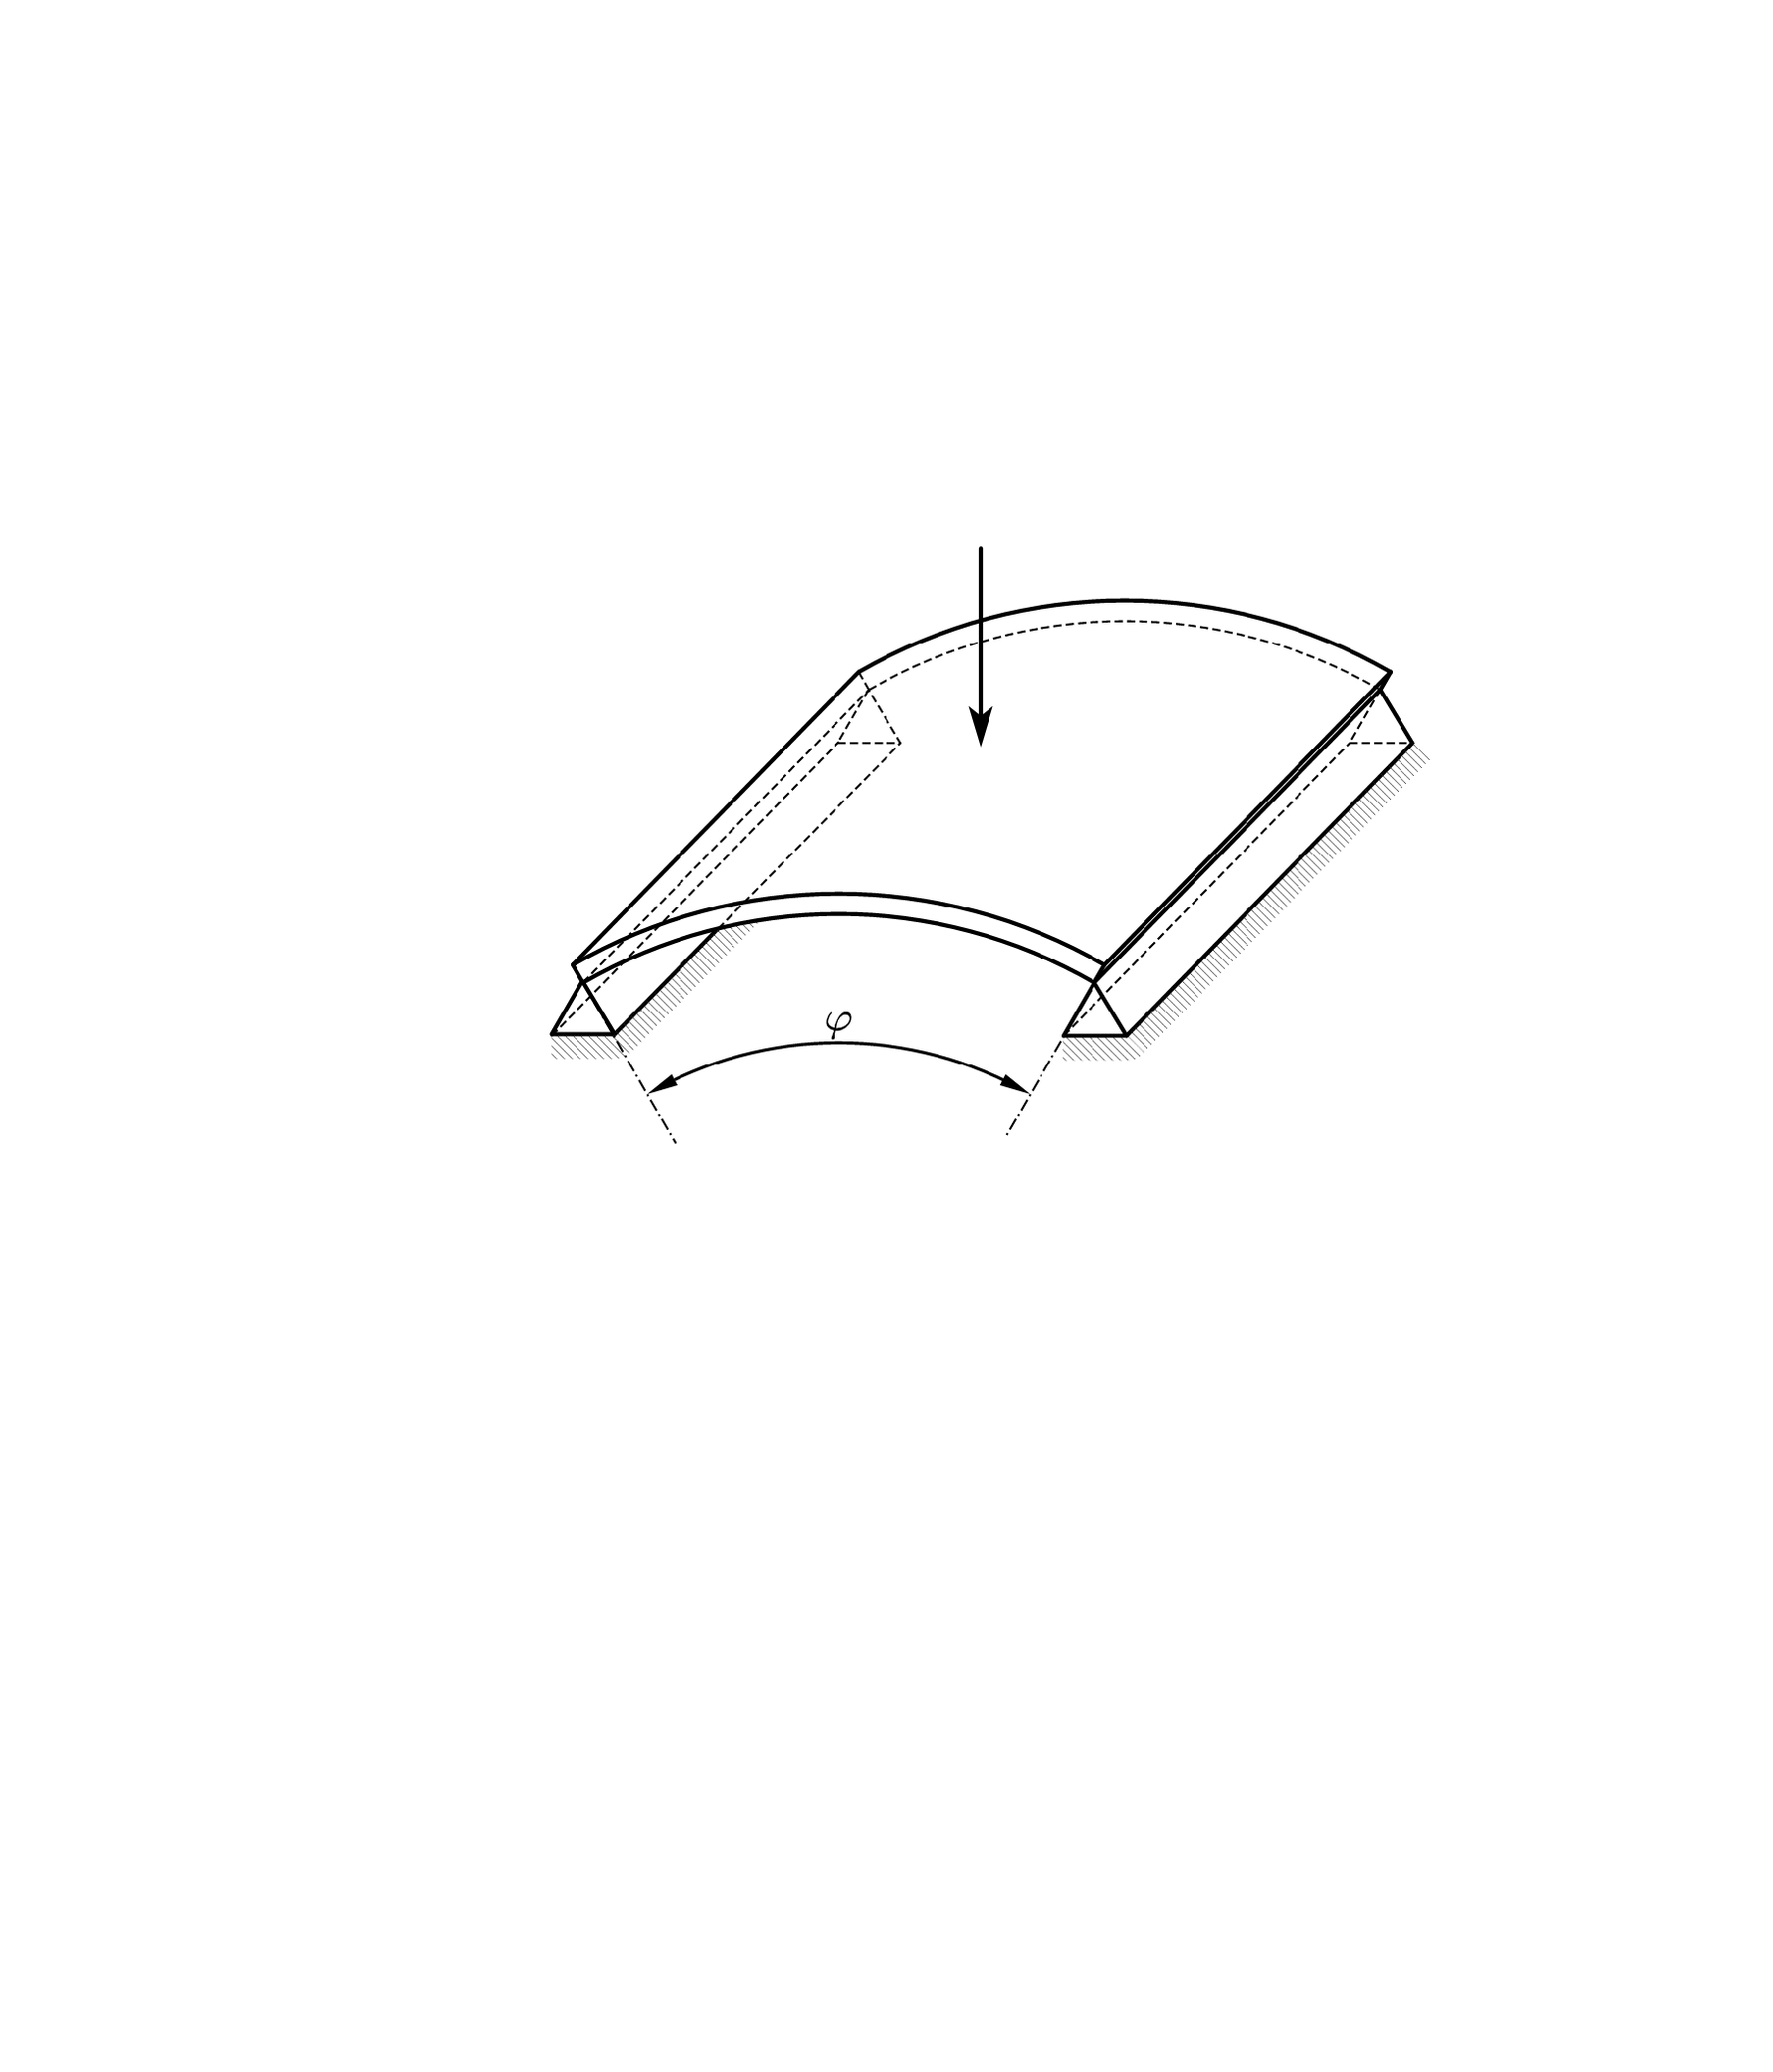
\includegraphics[height = 0.55\linewidth]{shell.pdf}
        \caption{两边简支圆柱薄壳}
    \end{subfigure}\bigskip
    \caption{板壳结构}
\end{figure}

\begin{marginpartext}
        板可以视作二维的梁,它同样主要承受横向外力。如果板足够薄,使得其几乎不能承受横向外力,就称其为膜。

        壳则是弯曲的板,由于几何形转是弯曲的,所以其受力平衡方程及动力学方程更加复杂。
\end{marginpartext}

\paragraph{弹性力学}

弹性力学是固体力学的基础,它研究一般弹性体在外载作用下的内力、变形情况。线弹性力学的基本理论早已建立,一些典型问题的解也已给出,也在此基础上分化出了材料力学和结构力学。目前,弹性力学有三个方向,第一个是与其他学科相互交叉,以研究多场作用耦合(如重力场、电磁场、化学场等多个场同时作用的力学系统)的力学模型;第二个是继续深化弹性力学的数学理论,研究非线性问题;第三个是研究弹性动力学理论,主要研究弹性体的振动及波的传播,这些内容在地震、地质勘探等领域有直接应用。

\paragraph{塑性力学}弹性体在受外力较小时,发生弹性变形,满足广义胡克定律,当弹性体受力超过其弹性极限后,其变形不再满足广义胡克定律,同时也会发生不可恢复的变形,这就是\uwave{塑性变形},而塑性力学就是研究弹性体发生塑性变形时,其变形与内力与外力之间关系的学科。塑性力学的主要研究内容有屈服条件、塑性增量理论和塑性本构关系。

\begin{figure}[h]
    \centering
    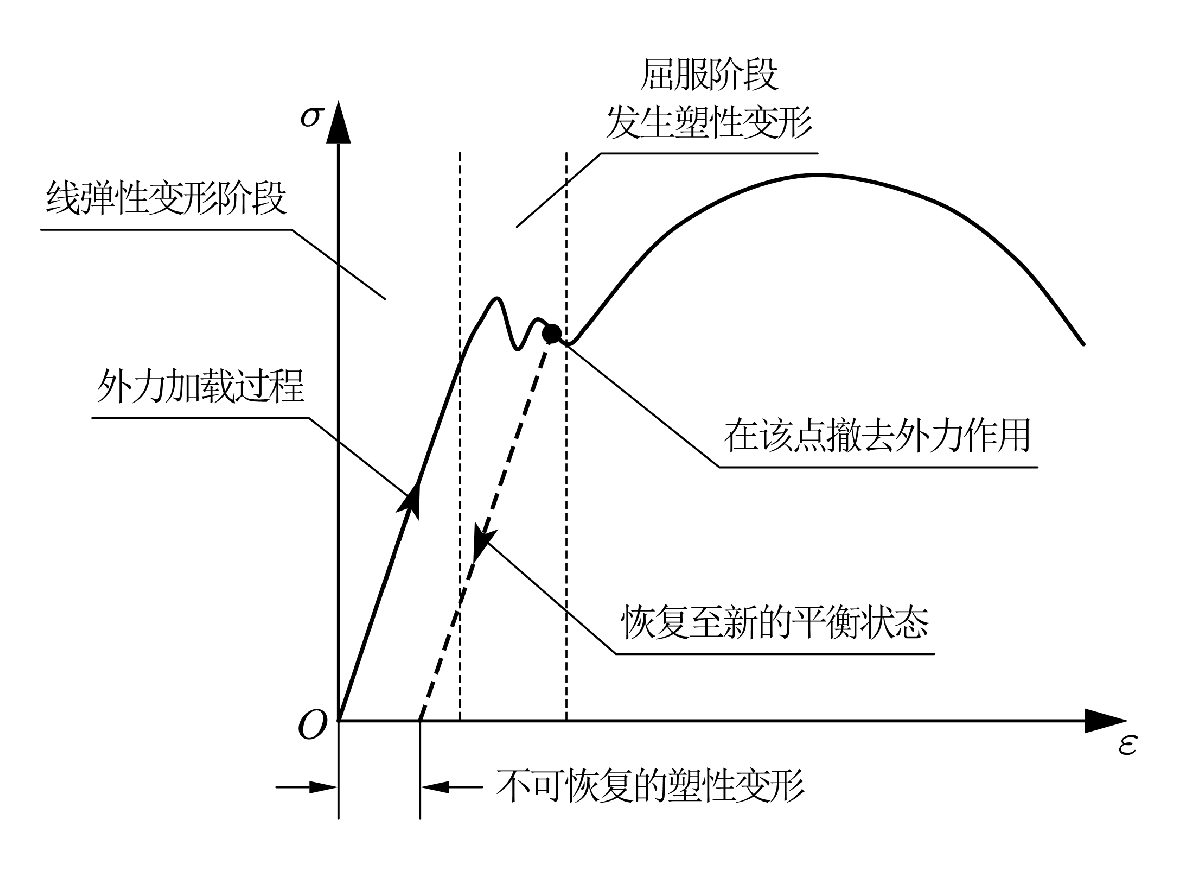
\includegraphics[width=9cm]{sigma_epsilon.pdf}
    \caption{塑性变形示意}
\end{figure}

\paragraph{断裂力学}

断裂力学是研究材料断裂失效和裂纹扩展规律的学科。该分支早期研究了裂纹扩展准则、裂纹尖端应力场分析、应力强度因子的计算方法等,以及如何将其应用到工程中去。目前的一些研究方面有:智能材料(压电、铁电等材料)的断裂与损伤、微纳米尺度断裂、非均质材料的断裂与损伤、断裂和损伤的试验与工程应用。

\begin{marginpartext}
        各向异性指的是某项物理规律与方向有关,同一位置处沿不同方向的物理规律不同。
\end{marginpartext}


\begin{wrapfigure}[8]{l}{5cm}
    \includegraphics[width=5cm]{carbon_fiber.jpeg}
    \caption{碳纤维复合材料管}
\end{wrapfigure}

\paragraph{复合材料力学} \uwave{复合材料}是由两种或以上不同材料经过特定工艺复合而成的新型材料,其性能往往比传统材料更优,且具有良好的可设计性。宏观来看,复合材料最典型的特征是弹性规律的各向异性		,因此复合材料问题往往也具有一定的非线性。目前,复合材料力学主要研究以下几个方面:复合材料基础力学理论、纤维增强复合材料的细观力学、特种环境复合材料力学性能模拟表征与优化设计、功能梯度复合材料。



\subsubsection{流体力学}

流体力学主要研究流体(主要是液体及气体)在外力作用下发生的质量、动量、能量传输。

\begin{figure}
    \centering
    \includegraphics[scale=0.5]{solitary.pdf}
    \caption{两孤立波相作用的图像($x$-位置,$t$-时间,$u$-幅值)}
\end{figure}

\paragraph{理论流体力学}

流体力学的基本方程已经建立起来,但是其求解是十分困难的。流体力学的基本理论有理想流体力学、粘性流体力学、空气动力学。目前只研究清楚了一些特定流动形式,一般的流动、湍流现象还是很棘手的。此外,流体力学还研究非牛顿流体及其应用、孤立波等问题。总之,主要研究的是较复杂的非线性问题。

\paragraph{工程流体力学}

工程流体力学包括很多分支,如水力学、气动力学、渗流力学、多相流等问题,所研究的问题往往具有较强的非线性,直接求解十分困难,往往要借助新的数值手段和实验手段。

\subsubsection{其他分支}

力学领域还有许多分支,如计算力学,可以与上述几个大的方向相结合,去研究对应领域中的计算、仿真方法;再如工程力学,关心实际工程问题中的力学问题,注重应用各种力学手段去解决工程技术、制造当中的问题;又如理性力学,通过基本公理和数学原理推导力学知识体系,力求严密性。此外,还有许多新兴的领域,属于力学与其他学科交叉,例如生物力学、机器人动力学、地球力学、岩土力学等等,限于篇幅不一一介绍。

\subsection{力学的研究方法}

对于一般的自然科学来说,研究手段很多,但是力学的主要研究手段只有三项:理论分析、试验测试与数值方法。

\subsubsection{理论分析}

理论分析是力学学科的传统分析手段。从假设出发,利用数学工具,建立模型的控制微分方程及边界条件,或者是积分方程。如果能求得解析解,那么就将其解析解求出来之后分析,也可以直接进行分析。

理论分析是力学与数学联系最紧密的部分,一方面,数学当中的定量分析对于准确描述力学模型而言是极为有用的;另一方面,对力学模型的研究也促进着数学的发展,这一点从牛顿建立微积分来研究经典力学起就是这样了,直到今天。

\subsubsection{实验测试}

实验与测试是考察我们所建立力学模型究竟是否符合真实世界中物体运动规律的手段。目前,实验手段是多种多样的,机械测量、光测、电测等方法,并形成了专门研究实验方法与手段的实验力学。随着新技术的发展,还有新的测量手段与方法不断涌现出来。


\subsubsection{数值方法}

\begin{wrapfigure}{l}{5cm}
    \includegraphics[width=5cm]{test.jpeg}
    \caption{测试试件基础力学性能的重要设备——万能试验机}
\end{wrapfigure}

数值方法是通过较为简单的代数运算方法,求出问题近似解的求解方法。一般来说,需要利用计算机进行辅助计算。

数值方法的主体就来自于计算力学,源自于早期的\uwave{有限差分法}(FDM)、瑞利-里兹法、伽辽金法,随着计算机的发展而兴盛起来,不断出现应用于各种问题的计算方法。目前,力学当中几乎各个领域的研究都离不开数值方法,数值仿真更是提供了一种节约成本的研究手段。对于一种数值计算方法,只有当其可靠性和效率都得到保证,才能算是成功的。一些比较成熟的数值仿真方法也已商用,在工程实践中发挥重大作用。例如,目前大多数商业计算力学软件中,处理固体力学问题的数值方法主要是基于\uwave{有限元法}(FEM)的,处理流体力学问题的数值方法主要是基于\uwave{有限体积法}(FVM)的。

\begin{figure}[ht]
    \centering
    \begin{subfigure}[t]{0.4\textwidth} \centering
        \includegraphics[height = 0.55\linewidth]{FVM.png}
        \caption{网格划分}
    \end{subfigure}\quad
    \begin{subfigure}[t]{0.4\textwidth} \centering
        \includegraphics[height = 0.55\linewidth]{FVM_solution.png}
        \caption{计算结果}
    \end{subfigure}
    \caption{计算模拟机翼附近空气流动}
\end{figure}

另外,近年来以数据驱动的研究方法逐渐被力学研究者采用,有人主张将其归类为新的研究手段,但这里姑且也将其划到数值方法之中,因为这种方法也是基于数值处理的,且离不开计算机和人工智能技术的发展。数据驱动指的是从初始的数据或观测值出发,运用启发式规则,寻找和建立内部特征之间的关系,也指基于大规模统计数据的处理方法。力学当中主要使用的还是机器学习手段,目前,有学者用机器学习的方法研究一些流体问题。
\restoregeometry
\section{专业数学培养}

 {\itshapeCJK
  数学是研究现代科学与技术的基本语言,力学更是工科之中与数学联系较为紧密的学科。掌握足够的数学知识是十分必要的,其意义不仅仅是为了应付考试,更在于掌握数学知识有助于准确地把握力学问题的本质,以及快速入门未曾研究过的专业问题,等等。学好力学的核心,除了培养力学专业的思维方式与直觉,最重要的便是要学好数学知识了。

  不过,学习任何一门学科都是需要付出很多精力的,特别是数学是一门对抽象思维能力要求较高的学科,学习起来的确有一定难度。所以我们最关心的问题自然是:如何学好数学?这其实是一个很大的问题,我们这里只能根据从笔者有限的经历,对学习的总体方法论和知识树作一简介,姑且算是给读者提供大致的理论指导。而读者则需要根据自身实践,对我们提供的指导思想做适合自己的调整,找到最适合自己的学习节奏。

  此外,力学的学习与数学的学习具有一定的相似性,有些方法是相通的,但我们着重介绍基础数学知识,对力学专业内容不做展开,还请读者在后续学习中自行体会与摸索。
 }

~\\

\subsection{总体方法论}

\subsubsection{培养自学能力}

大学教育与中学阶段的最显著的区别是,授课教师不会像以前一样手把手地教,把所有的知识点都嚼碎之后喂给我们。实际上,大学设置课程的质量参差不齐,如果只是一味地跟着授课教师亦步亦趋,往往是学不到多少东西的。同时,在以后的研究、工作之中,很多事情也都需要自己去想办法解决。所以培养自学能力就十分重要了。那么,如何培养自学能力?

\paragraph{兴趣是最好的老师}

作为一名理工科学生,在学习过程中会用到很多数学。微积分、线性代数等等不一而足,然而对于力学系的同学来说,计算能力和建模应用是首位的,逻辑上的推理以及严格性的证明往往是被我们作为学习数学辅助手段来使用的。

力学系的同学使用数学工具的过程中,常常会对自己使用的数学工具产生疑问,这样做是否是合理的?为什么会是这样?为什么有的地方满足交换律,到了别的地方就不满足了?同样是两个方程确定的偏导数,为什么在表达顺序上会出现异常的规律?$x$ 和 $y$,究竟在哪里等价,在哪里又不等价?深入的思考带来的疑问,驱使着我们去发现未知的数学规律,而在这个过程又会带来极大的愉悦和满足。从工科的角度学习数学就是这样一个过程,从使用中产生疑问,在解答疑问的过程中产生新的想法。大学毕业以后,有些专业课有可能以后很难再接触到,真正珍贵的是自己独立思考的过程,和灵光一现,再到解决疑问的愉悦感。

在大学里,建立良性的循环是非常有必要的。什么是良性的循环?不妨先看看什么是恶性的循环。假如你有一天熬夜到很晚,第二天跟不上老师,下课后作业不会,费尽心思搞懂又是深夜。在这个过程中一点点磨灭掉自信心,从此开始摆烂,直到挂科,退学等等事情的发生。规律的作息是保证良好心态,形成良性循环很重要的一部分。而良性循环就刚好相反,比如学习——兴趣——思考——学习的过程,这样的循环对于坚持学习是非常重要的,学习的开始往往是从兴趣开始的,这也是为什么兴趣是最好的老师。

\paragraph{资料与信息检索}

\begin{enumerate}
    \item 善用图书馆。如果将图书馆只是当作自习室,那实在是暴殄天物。对于一个大学生来说,图书馆有着最直接也最好用的海量图书资源。你可以在图书馆借到大量的、侧重点各不相同的同一类书籍。有些大学的图书馆会有许多国外的或者国内已经绝版的、甚至是独一无二的优质资料。不夸张的说,图书馆至少能够满足一般人在本科阶段大多数的资料需求。同时,善用图书馆的检索功能,掌握书籍的检索规律,还能锻炼资料检索的能力。
    \item 电子资源的检索。Zlib、知网、Sci-Hub、学校图书馆的线上借阅、各种不知名的小网站、百度网盘等等都藏有许多资源,这种资源检索往往需要对所研究的领域有一定了解。在入门阶段,不妨应用百度、知乎、Google、CSDN等检索平台,对于某些领域来说能够满足快速入门,获得一个初步印象的需求。
          关于更多的具体的数学检索平台,可参见USTC基础数学修课指南。
    \item 充分调动人脉资源。很多时候,我们缺少的往往是获得关键信息、资料的途径,这些内容不是通过阅读已有书籍或电子资料就能获得的。这时候,要积极地向身边或线上了解相关领域的朋友请教,他们手中的资料、他们对于该领域的见解,都是相当宝贵的信息,这要比自己探索方便快捷得多。但是,如果有志于独立研究,也不要过分依赖于他人的帮助,因为总有一天会面临无人可问的情形。
\end{enumerate}

\paragraph{正确处理习题,形成自我评估}

对于习题的争论,历来分成两派,一派主张“题海战术”,另一派与之相反。究竟应该选择哪一种,取决于学习动机。

对于应试来说,“题海战术”确实是行之有效的方案。但对于一般性的学习,我们不建议直接捧着习题集做,却也不是少做题。在反对“题海战术”的思潮中,也有另一种极端,即动笔很少,这也是不可以的。题必须要做,只是最好要有选择性地做、精做。做题的主要目的有两个:一是通过操作实例,积累经验与直觉,所以像《吉米多维奇》这样习题重复度过高的参考书并不值得大家花时间去大做特做;二是检验学习程度,判断目前的水平是否可以继续深入学习,只有打牢基础才能钻研更深入的知识,前置知识掌握得不牢固,学习后续知识就容易出现困难。

如何做题也是有讲究的。首先,尽量选择有参考答案,最好是有详细解答步骤的题目去做。其次,在做题时,独立思考是很重要的,但也不要受“独立思考”这种说法的束缚,题目中某个关键步骤如果想了很长时间也没想出来,就应该直接去看答案了。我们的目的是掌握方法,把答案看懂(而不是囫囵吞枣)当然能够掌握方法,没必要有什么心理负担,我们如今所学的知识都是前人经过数十年、数百年浓缩而成的,把所有细节全都背下来,既是不现实的,也是没必要的。

\paragraph{快速入门学科,不必万事俱备}

在学习和科研的过程中,我们常常有快速入门一个学科/领域的需要。要想快速入门一门学科,最好还是直接看问题,从问题下手往往是最快的,因为这时有足够的动机。不必管解答,无论能否看懂,起码都会先有一个印象,以及自己思考的过程,这样就可以算得上入门了,入门之后再去考虑其中的细节问题。

比较忌讳的是为了一个领域/专业课,去大学特学前置知识。一来这样效率低;二来准备得完全充分也是不现实的,在学习和研究的过程中经常会出现新的概念,现用现学才是常态;三来是不同专业的侧重点不完全一样,如果学了某样“前置知识”,到最后发现在专业课的实际应用中并没有用到那么多知识,就有点得不偿失了。

此外,快速入门的另一个前提是要有广泛的知识储备,也就是说在一定程度上当一个“名词党”是有好处的。不管怎么说,知道有一个名词比不知道强,在前期调研时至少有一个大致方向。第一次接触某一个名词时,不一定要对其有多么深入的理解,哪怕仅仅是形式上接受它也未尝不可。

\paragraph{学数学是一个积累的过程}

很多人可能会认为,理工科类型知识的学习只要捋顺逻辑即可,无需进行记忆。事实并非如此,倒不是说我们需要去背公式、记习题,而是要积累观点、思想方法和典型例子。“数学成熟度”是一个比较玄学的指标,看不懂书的时候,可能有人会对我们说:“这是数学成熟度不够导致的”。“数学成熟度”大概指的就是我们习惯一套数学语言的程度,我们在数学上做积累的目的就是提高“数学成熟度”。

如何提高“数学成熟度”呢?凡事没有捷径,唯一的捷径就是抛开杂念去做。数学的学习,分为输入和产出的过程。看书、做题、上课是输入,与人交流、整理笔记、编写讲义、写小论文等是输出的过程。数学思维的建立不是技巧的堆砌,而是积累大量的数学观点和思维方式,能说出定理和定理、学科与学科之间的关系。循序渐近,多看、多写、多想,才能逐渐提高“数学成熟度”。这是一个或长或短的积累的过程,不必急于求成,踏实去学才能厚积薄发。

\paragraph{一些学习方法}

在学习过程中,还有一些具体的方法:

一定要充分发挥主观能动性,我们的目的是学知识,不是折磨自己。这意味着可以先通读学习材料,先对知识形成一个整体印象,遇到不懂的一个点可以选择性地跳过,待通读若干遍之后,再精读,去认真考察其中的细节。这也是一般阅读文献应该采用的思路。

抄书是自学的有效方法。它可以是选择性地摘录重点,也可以是事无巨细地誊写,抑或是学习一遍后的总结、归纳。这种方法看似笨重无比,实际上是能稳定获得较大收益的办法,抄书能辅助你集中注意力,完成构建知识体系的过程。

若是比较关心数学的力学应用,则不必限于技术性细节,更多地关注计算与应用。可以选择性地忽略一些严谨的证明,暂时接受一项结论,在具有一定理解的前提下考虑如何去计算和应用,通过不断地计算和应用反过来加深对概念的理解,这既包括对数学概念本身的理解,也包括概念及相关的计算方法可以被应用在哪些物理和力学模型下,在有进一步需要的情况下,可以考虑花些时间仔细地研读证明过程。

若是出于兴趣,或是为了学习一些高级的数学理论和工具,请一定打好前置知识的基础,关心问题的处理思想与方法,关键性的推理与证明都不要放过。很多进阶的概念和方法是从比较基本的问题中提炼、概括出来的,对基本背景问题有足够的了解,能更好地理解提出某项概念或定理的动机,以及了解其研究思路,处理一些问题时能有一个大致的思路。

\subsubsection{形成认识与对待数学的观点}

之所以单独开设这一个板块,是因为笔者发现即使到了本科毕业的时候,仍然有许多专业内的同学没法分清数学和物理/力学之间的区别。这源自于我们中学阶段对数学基础的忽视,而只是简单归纳“性质”、“应用”造成的恶果,如果延续这种“一叶障目,不见泰山”式的思维进行学习,是走不长远的。很多人学了数年数学和物理,只能看到“数学和物理当中都有很多定理、公式”、“都需要做大量计算”,却难以分辨出二者之间除了研究对象以外的区别,只是觉得数学似乎更抽象一点,物理/力学更实际一点,实际上这是浅显的、片面的。

最重要的区别在于,数学不是自然科学,而是形式科学,而物理/力学都是自然科学。自然科学是一门以观察和实验的经验证据为基础,对自然现象进行描述、理解和预测的科学分支,就是说自然科学要取之于实践,终究也要用之于实践。形式科学并不关心真实世界与理论之间的联系,而关注以定义和规律为基础的形式系统的性质。

数学作为形式科学的属性决定了,在数学当中,只要推理是正确的,那么得到的结果就一定是正确的,不存在任何更改的余地,一旦需要修正,一定是推理出现问题,或者需要相应修改推理的前提。而在自然科学中,所有理论都是通过观察、归纳,总结出基本定律之后获得或再推理获得的,观测和归纳出现问题,都可能导致理论的修正。同时,数学也可以作为一种语言对自然科学进行定量描述,构建数学模型对实际问题加以研究,正是这一原因容易使人们看不清数学与自然科学之间的关系。

时常有人对数学发出诘难:“数学有什么用?”,然而数学作为形式科学本就不必考虑实用性,以及现实世界是什么样子的,它可以是纯粹的思维游戏,这无可非议。可是,数学又不能完全脱离实际。这话看起来有些矛盾,但一切抽象的知识和问题最初都一定来源于实践,只是经过不断地归纳、总结、抽象、一般化的过程中,我们可能已经看不出问题原来的模样。

不过作为力学专业的学生,我们更多地是把数学作为描述力学问题的语言与解决力学问题的工具。如果拿作战做一个比喻,我们的力学原理和直觉就像是战略与战术思想,指引我们的研究方向,而数学就像是支持作战的后勤保障,支持着研究进行以及这场研究能够走多远。

抽象也好,实用也罢,研究抽象数学理论和研究数学理论与现实情况之间对应关系的数学家都应该得到我们的尊重,他们从事的是人类头脑所能进行的最伟大、最艰深的活动之一。

\subsubsection{正确处理数学与力学专业的关系}

\paragraph{注意学习数学的动机}

在确认学习之前,一定要明确学习动机。学习数学应当以力学专业课程为导向,兴趣爱好为辅,无需过早地接触过于抽象的数学。我们当然支持出于兴趣学习一些高级的数学工具,而且这也是有好处的,但是一定要避免在这个过程中形成眼高手低、浮于表面的坏习惯。

我们指出,所谓高级工具本质上更接近对“相对初级”的理论的归纳、抽象、推广,有些高级工具需要学习到足够深入之后才能拿来解决一些问题,这对于力学学科来说的代价很大,务必做好取舍。也有些高级工具压根就不是为了解决现实问题服务的,或者说至少不是为了你感兴趣的领域准备的,这时也需要考虑清楚学习成本。

再者,务必端正深入学习的动机。中学阶段的应试教育培养出了一种奇怪的思潮,即所谓“应用高级数学工具对初级问题进行‘降维打击’”。经验表明,高级数学工具往往并不会直接产生“降维打击”的效果,它起到的通常是提供思路的作用,甚至可能不起作用,换句话说,通过高级工具实现“降维打击”的收益至少不明显大于打好基础的收益,“降维打击”并不是高级工具应有的作用。熟悉了高级工具之后,应该做的是去了解更广泛的数学、应用知识,在反复使用中熟悉、理解、内化,将“高级工具”变成你的“初级工具”,这才是“高级工具”正确的打开方式。

另外,如果出于应急所需,例如一门专业课要用到某样数学工具,这时也不建议直接去找一本数学理论性很强的书去看。因为数学方向与专业所需的关注点可能并不一样,这样不仅见效慢,而且更可能打击自信心,为学习徒增障碍。更好的做法是边学专业内容边补数学工具,以及找一些有附录讲解这些工具的同类书籍,在有了基础知识和专业知识后,如有兴趣,可以考虑再看相应的数学理论。

\paragraph{注意学习数学应该深入到什么程度}

力学学科与数学的联系是相当广泛的,乍一看学习力学需要特别多的数学,但实际上所有内容的基础都是微积分与线性代数,这是一切学习的根本与下限。出于不同的学习动机,学习的深入程度自然也是不一样的。

如果只是为了应付考试、科研,那掌握最基本的微积分和线性代数可能就足够了。但是,这时去备考或阅读文献可能会比较痛苦,因为很多数学概念是有更深厚的数学或物理/力学背景存在的,如果不能把握这一点,那么所做的工作可能会显得比较破碎、凌乱,不容易直击问题要害。

如果为了在科研中取得一定成果,或者对数学有一定兴趣,那么至少本科数学基础课都应该学好。我们后边将会介绍,本科阶段的基础数学课都是有用的,会在某些力学课程中用到,只会微积分和线代的话,就算能看懂,理解起来也会存在很大障碍。

如果为了专门处理某类问题,或者对某一数学领域兴趣浓厚,则应该广泛地参考课外学习资料。这个阶段不必限于培养方案中的设置,根据自己的需要、兴趣广泛地学习即可,但也要注意深入的程度,没有必要学习相当抽象的理论,仍然以计算和应用为主。(除非是确实对抽象的数学理论感兴趣,但若是如此,请自行平衡好时间和精力)

\paragraph{注意寻找与建立数学与力学之间的联系}

学过相应的数学后,一定不要束之高阁,而要寻找和思考这些数学工具可以用在哪些地方。知识只有在不断运用之中,才能得到深层次的理解,长时间不用自然会遗忘。具体的联系我们将在具体的数学科目中介绍。


\subsection{基础数学培养}

\begin{figure}[ht]
    \centering
    \includegraphics[width = \textwidth]{TREE.pdf}
    \caption{力学系的数学科技树}
    \label{fig:力学系的数学科技树}
\end{figure}

前一节业已提及数学的重要性,以及如何把握数学知识。本小节将介绍大学内最基本的数学知识——微积分及线性代数,以及其相关知识的基本外延。微积分和线性代数是描绘一切理工类学科知识以及进阶数学知识的基础,其重要性不言而喻,一定要给予足够重视。然而,如何有针对性地学好这两门基本数学课程,使之与日后专业知识的学习相适配,不同专业又有不同的侧重点,这里我们只勾勒力学类学生应该需要把握的大体框架。

总体而言,由于这一部分的数学课程最基础,同时也最重要,所以这一部分即使不是出于应试需要,也建议稍多做一些习题,确保对这些基础知识和处理技巧有足够的熟练度。

具体的介绍之前再次强调,我们所讲的内容不以应试为导向。

\subsubsection{微积分}

\paragraph{主体知识介绍}

微积分是研究\uwave{微分}和\uwave{积分}是数学分支。粗略地说,微分讨论的是“变化率”,积分讨论的是“累积”或“求和”。在力学上有两个经典的例子分别给出了研究微分与积分的动机:为了计算物体在运动过程中某一点$M_0$处的瞬时速度,再取一点$M$,能算出这段路程上的平均速度,当$M$足够接近$M_0$,这个平均速度就能近似描述瞬时速度,这个过程就是微分;为了计算物体在变力作用下运动过程中所做的功,先将运动轨迹分成若干段,在不同段上用分别用一个常力代替变力计算做功功,随后求和,当运动轨迹划分得足够细致时,计算的结果就近似于真实的做功大小,这个过程就是积分。

\begin{figure}
    \centering
    \includegraphics[width = \textwidth]{differential.pdf}
    \caption{当$M_0$运动到$M$的时间$\Delta t$足够小时,$\symbfit{v}=\dfrac{\Delta \symbfit{r}}{\Delta t}$就近似表示瞬时速度$\symbfit{v}_0$}
\end{figure}

\begin{figure}
    \centering
    \includegraphics[width = \textwidth]{integral.pdf}
    \caption{力$F$在$x$轴上运动,从$a$到$b$所做的功}
\end{figure}

学习微积分首先要有\uwave{数列}和\uwave{函数}的概念,函数研究的是变量之间的变化关系,数列可以看成定义域离散的函数。在正式学习微积分之前,要对基本初等函数有一个了解,知道其基本性质、函数图像。

一元微积分研究的是一元函数的微分与积分,其基础是\uwave{极限}理论。

一元函数微分部分的核心技巧与内容有两块:\uwave{Taylor公式}与\uwave{微分形式不变性}。Tay-lor公式是描绘可微性足够好的函数在某点附近性质的有力工具,所以要对各种基本初等函数的Taylor公式相当熟悉,同时,它也是对“等价无穷小”这一概念的更精确的表述,能够回答“极限中函数什么时候可以做加法”的问题。微分形式不变性是能将\uwave{复合函数链导法则}、\uwave{隐函数求导}等内容串到一起的,从这里出发能将前边所学的很多东西联系起来。

\begin{figure}
    \centering
    \includegraphics[scale=0.5]{Taylor.pdf}
    \caption{$y=\sin x$及其前几阶在$x=0$处的Taylor展开图像,展开项越多,在$x=0$附近越接近$y=\sin x$}
\end{figure}

关于微分需要多说一点。有些教材上对于微分的处理很模糊,较好的教材会说“微分是函数变化过程中的线性主部”,我们在此阶段,不妨就把微分看成是差分的极限。在处理一阶导数时,可以在形式上将其视为$\mathrm{d}y$与$\mathrm{d}x$的商,但是高阶导数则不行,也因此“反函数的导数是原本函数导数的倒数”这一奇怪的结论(实际上,基于微分形式不变性就能求解反函数的导数)仅能对一阶导数成立。在后续的学习中,也能看到“将微分看作某个线性空间下的基”这种观点,那是后话了,多数时候将微分看成差分的极限是够用的。

另外,涉及到无穷的讨论一定要慎重,从对有限的讨论结果直观外推的结果不一定可靠,必须要做严谨的分析!这一观念在后续课程中是很重要的。

一元函数积分比较重要的内容是\uwave{分部积分}
\[
    \int_{a}^{b} u(x)v'(x)\,\mathrm{d}x = u(x)v(x)\bigg|_a^{b} - \int_{a}^{b} u'(x)v(x)\,\mathrm{d}x
    .\]
以及\uwave{Newton-Leibniz公式}
\[
    \int_{a}^{b} F'(x)\,\mathrm{d}x = F(x)\bigg|_a^{b} = F(b)-F(a)
    .\]
不定积分运算是已知导数求原函数的过程,它与导数运算在相差一个常数意义下是互逆的。正如在正数的范围内引入减法会产生负数、在整数的范围内引入除法会产生有理数,初等函数的不定积分也会产生不属于初等函数的函数。事实上,绝大多数的初等函数的不定积分都不是初等函数,所以能够掌握一些基本的、常见的不定积分技巧,包括换元、分部积分即可。而分部积分是很重要的,这个技巧在涉及到能量的方法以及变分法中是常用的。Newton-Leibniz公式的精髓不只在于建立了函数及其导数的关联,它还建立了区间和区间边界的联系,这一点在多元积分当中的各种积分公式中也能够看到。


\begin{figwindow}[0,r,
        {\includegraphics[width=4.5cm]{partial.pdf}},
        二元函数$z=z(x,y)$的偏导数]
    多元函数微分部分,首先要掌握$n$维欧氏空间$\mathbb{R}^n$中的诸多基本概念(拓扑性质),这些基本概念在后续学习中还会用到。最重要的概念当属\uwave{偏导数}与\uwave{全微分},偏导数只描述函数关于某一个自变量的变化情况,而全微分反映各个自变量的影响,因此全微分比偏导数要强很多。类似一元微分学部分,全微分也具有形式不变性,同时也能搞定复合函数求导以及隐函数求导。这里可能要注意不同学科的习惯不同,比如力学中,设有一个函数形式为$L=L(q(t),t)$,若要求其对时间$t$的全导数,往往会写成以下形式:
\end{figwindow}

\[
    \frac{\mathrm{d}L}{\mathrm{d}t}=\frac{\partial L}{\partial q}\frac{\mathrm{d}q}{\mathrm{d}t}+\frac{\partial L}{\partial t}
    .\]

形式上看,这种记法符合全微分形式不变性,但数学上可能记$L=f(q(t),t)$,其对$t$的全导数为

\[
    \frac{\mathrm{d}L}{\mathrm{d}t}=\frac{\partial f}{\partial q}\frac{\mathrm{d}q}{\mathrm{d}t}+\frac{\partial f}{\partial t}
    .\]

没有哪一种写法是错的,只要注意不同的习惯约定即可。多元函数微分学常用一些空间解析几何的内容,在此之前最好先学习一下相关内容,知道常见空间曲线、曲面的解析式。另外,从这里开始逐渐接触到一些涉及到\uwave{梯度场}的知识,由于数学工具限制,在这一阶段不会太过深入,知道一些关键结论和初步应用即可。

多元函数积分与场论部分,首先要熟悉基本的累次积分、二、三重积分的计算,以及不同坐标系下积分微元的关系。随后是两类曲线 / 曲面积分,第一类曲线积分主要注意选择合适的参数将弧微元转化成关于参数的一重积分,第一类曲面积分主要注意选择合适投影面将面微元转化成关于两个坐标的二重积分。第二类曲线 / 曲面积分是矢量积分,一方面注意其与第一类曲线 / 曲面积分的联系,另一方面注意\uwave{Green公式}、\uwave{Gauss公式}、\uwave{Stokes公式}\footnote{可以看到,Green公式、Gauss公式、Stokes公式与Newton-Leibniz公式类似,都将函数及其导数,以及区域及其边界联系了起来。}
\begin{gather*}
    \iint_{\sigma} \left(\frac{\partial Q}{\partial x}-\frac{\partial P}{\partial y}\right)\mathrm{d}x\,\mathrm{d}y                                                                                                                                                                                                     = \oint_{\partial \sigma} P\,\mathrm{d}x+Q\,\mathrm{d}y,                                                        \\
    \iiint_{\Omega} \left(\frac{\partial P}{\partial x}+\frac{\partial Q}{\partial y}+\frac{\partial R}{\partial z}\right)\mathrm{d}x\,\mathrm{d}y\,\mathrm{d}z                                                                                                                                                         = \oiint_{\partial \Omega} P\,\mathrm{d}y\,\mathrm{d}z+Q\,\mathrm{d}z\,\mathrm{d}x+R\,\mathrm{d}x\,\mathrm{d}y, \\
    \iint_{\Sigma} \left(\frac{\partial R}{\partial y}-\frac{\partial Q}{\partial z}\right)\mathrm{d}y\,\mathrm{d}z+\left(\frac{\partial P}{\partial z}-\frac{\partial R}{\partial x}\right)\mathrm{d}z\,\mathrm{d}x  +\left(\frac{\partial Q}{\partial x}-\frac{\partial P}{\partial y}\right)\mathrm{d}x\,\mathrm{d}y = \oint_{\partial \Sigma} P\,\mathrm{d}x+Q\,\mathrm{d}y+R\,\mathrm{d}z.
\end{gather*}

的运用。此外,此处会进一步涉及\uwave{散度场}、\uwave{旋度场}的内容,需要熟知\uwave{梯度算子}\;$\nabla$的基本计算,以及“有势无旋、有旋无源”等常用的结论。

一般的微积分教材还会有两个专题,一是\uwave{常微分方程},二是\uwave{无穷级数}。微积分课程中所讲的常微分方程是比较有限的,最重要的当属\uwave{常系数线性微分方程}和\uwave{Euler方程},我们重点关注其求解。无穷级数中最重要的是\uwave{Taylor级数}和\uwave{Fourier级数},Taylor级数部分注意运用运算规则推导常用的级数,Fourier级数部分在计算Fourier系数时,常用分部积分的技巧。

\begin{wrapfigure}{r}{5cm}
    \includegraphics[width=5cm]{inertia.pdf}
    \caption{转动惯量示意}
\end{wrapfigure}

\paragraph{与力学专业内容的联系}
微积分将伴随我们后续整个学习生涯,几乎没有哪一个力学专业课用不到微积分,我们只介绍几个典型应用。
\begin{itemize}
    \item 质心与转动惯量——重积分
          \[
              \symbfit{r}_C=\dfrac{\int_\Omega \symbfit{r}\,\mathrm{d}m}{\int_\Omega \mathrm{d}m}, \quad J_l=\int_\Omega d^2\,\mathrm{d}m
              .\]
    \item 建立连续体平衡微分方程——微元法
          \[
              \tau_{xy} = \tau_{yx}\quad \text{\itshapeCJK(切应力互等)}
              .\]
    \item     弹性力学中轴对称问题应力函数所满足的方程
          \[
              \left( \frac{\mathrm{d}^2}{\mathrm{d}\rho ^2}+\frac{1}{\rho}\frac{\mathrm{d}}{\mathrm{d}\rho} \right) ^2\varPhi =\frac{\mathrm{d}^4\varPhi}{\mathrm{d}\rho ^4}+\frac{2}{\rho}\frac{\mathrm{d}^3\varPhi}{\mathrm{d}\rho ^3}-\frac{1}{\rho ^2}\frac{\mathrm{d}^2\varPhi}{\mathrm{d}\rho ^2}+\frac{1}{\rho ^3}\frac{\mathrm{d}\varPhi}{\mathrm{d}\rho}=0
              .\]
          ——Euler方程

    \item  信号频谱分析——Fourier级数,见 \autoref{fig:一种信号的时域与频域关系对应图}
\end{itemize}



\begin{figure}
    \centering
    \includegraphics[scale=0.45]{Fourier_series.pdf}
    \caption{一种信号的时域与频域关系对应图}
    \label{fig:一种信号的时域与频域关系对应图}
\end{figure}

\paragraph{学习建议}

我们以后的运用以计算为主,如果初学时对一些严格定义有困惑,可以在不影响计算与运用的前提下适当放一放。在能进行计算的前提下,回头结合计算实例进行理解。

以计算为主不代表要去算各种奇奇怪怪的极限、积分。如果没有准备竞赛的要求或是出于个人兴趣爱好,没有必要算那些奇怪的积分(特别是有些来路不明的钓鱼题)。一来,能够计算出结果的积分是十分有限的,更可能要用到许多特殊函数的性质;二来,我们以后会用数值方法去处理广泛的积分,若非分析性质的需要,数值解是足够的。

一般微积分课程中对于矢量分析的内容是不足的,这里可以做一些额外补充,否则面对普通物理学当中的力学推导,以及理论力学当中的运动学部分的推导可能会比较吃力,推荐书目有 \textcite[托马斯大学微积分]{李伯民2009托马斯大学微积分} 的10、11两章,\textcite[数学分析新讲]{张筑生数学分析},\textcite[工程数学——矢量分析与场论]{谢树艺2015工程数学} 的前2章。

\paragraph{参考书目}

参考书选择大前提:一定要适合自己,不要三人成虎,先入为主地迷信或厌恶某本教材!学习过程中可广泛参考不同教材,但应该以其中一两本为主,其余为辅。

首先,同济大学的《高等数学》能够满足正常的微积分知识学习,包括很多高中参加物理竞赛的同学学习高数时也参考了这本书。这本书的例子、逻辑与习题量至少能满足力学专业的学习,如果要参考其他教材,请至少以此为下限进行参考。这套教材最大的问题是过于中庸,虽然有例子但不够丰富,逻辑性与严密性卡在一个比较尴尬的位置。

\begin{itemize}
    \item 入门级参考书:

          \begin{center}
              \includegraphics[scale=0.6]{book/1.png} \quad
              \includegraphics[scale=0.6]{book/2.png} \quad
          \end{center}

          \begin{itemize}
              \item \textcite[普林斯顿微积分读本]{杨爽2010普林斯顿微积分读本}

                    入门级微积分读本,适合没有相应数学基础的高中生以及文、史、哲、法学生阅读,主体内容是一元微积分的部分。这本书的特点是起点足够低,对于基础内容的讲解也足够细致,不一味强调严谨性,因而适合初学者入门。问题在于内容较浅、过于冗杂,这种风格并不适合一般理工科的后续学习和科研要求。

              \item \textcite[托马斯大学微积分]{李伯民2009托马斯大学微积分}

                    入门级微积分读本,基本涵盖了国内一般微积分教材的大部分内容。特点是起点低,知识点引入比较流畅,内容丰富,实例、图示与习题都很充足,也很适合初学者入门。
                    后续的数学课程帮助很大。
          \end{itemize}

    \item 进阶与拓展参考书:
          \begin{center}
              \includegraphics[scale=0.35]{book/5.png} \quad
              \includegraphics[scale=0.35]{book/3.png} \quad
              \includegraphics[scale=0.56]{book/4.png}
          \end{center}
          \begin{itemize}
              \item \textcite[数学分析新讲]{张筑生数学分析}

                    这一套书作为数学分析来说,没有在集合论和实数上大书特书,更多地是从计算以及几何意义的角度进行引入。对于书中提及的拓扑和一般线性空间的内容,只需要粗略扫过,有一个印象即可。书中对于多元微积分的处理,曲面以及曲线积分的计算,矢量微分算子的引入都是非常有借鉴价值的,尤其是微分方程部分,包括常微分方程和简单的偏微分方程理论,对学习后续的数学课程帮助很大。

              \item \textcite[工程数学——矢量分析与场论]{谢树艺2015工程数学}

                    这本书在微积分水平上对矢量分析进行了比较全面的讨论,第一章讨论了矢量函数的微积分,后边讨论了矢量场、梯度算子及一般的曲线坐标系中的运算,对于本科课程级别的运动学、弹性力学和流体力学中的矢量运算比较有帮助。

              \item \textcite[微分几何]{彭家贵2002微分几何}

                    这本书所讲的第一部分是古典微分几何的内容,适合在学了微积分之后适当阅读。涉及的数学工具只有微积分、空间解析几何及少量的线性代数,理论不抽象,计算较复杂,同时,工程力学的研究大都是在经典的三维欧氏空间$\mathbb{R}^3$下的,所以这本书正适合力学专业的同学阅读。

                    古典微分几何大致可分为曲线论和曲面论。曲线论的研究方法可以追溯到对质点运动轨迹的研究,比较有意思的是标架方法,学过这一部分内容之后正好可以重新审视一下质点运动学的内容。曲面论的内容相对比较丰富,一般来说会先从曲面的基本形式和曲率入手,通过活动标架方法,研究曲面的结构方程,最后是曲面的内蕴几何学及测地线的理论。
          \end{itemize}
\end{itemize}


\subsubsection{线性代数}

\paragraph{主体知识介绍}

线性代数以研究\uwave{线性变换}、\uwave{线性方程组}为主。在数学上,\textbf{线性}一般指的是\uwave{齐次性}和\uwave{可加性},例如对于映射$f:\mathbb{R}^n\to\mathbb{R}$,这两条性质指的是

\begin{itemize}
    \item 齐次性:$f(a\symbfit{x})=a\cdot f(\symbfit{x})$.

    \item 可加性:$f(\symbfit{x}+\symbfit{y})=f(\symbfit{x})+ f(\symbfit{y})$.
\end{itemize}
这时就说映射$f$是线性的。研究在有限维线性空间(例如$n$维欧氏空间$\mathbb{R}^n$)中线性变换的代数性质的分支就是线性代数。那么典型的线性变换有哪些呢?我们举平面解析几何中的两个例子说明。

设平面上有一点$(x,y)$,现在将其绕原点逆时针旋转$\theta$度,利用三角函数的诱导公式容易得到变换后点$(x',y')$的坐标为
\[
    \begin{cases}
        x'=x\cos \theta -y\sin \theta, \\
        y'=x\sin \theta +y\cos \theta.
    \end{cases}
\]
不妨将点$(x,y)$看作是矢量$(x,y)$。在这里看来,齐次性就是在变换先后将向量$(x,y)$拉长若干倍;可加性可看成将向量$(x,y)$拆成$(x,0)$与$(0,y)$之和,将二者分别逆时针旋转$\theta$度后再加和,得到的结果与直接旋转向量$(x,y)$是一致的。所以,这种旋转变换是线性变换。

\begin{figure}[h]
    \centering
    \includegraphics[width = 0.8\linewidth]{homogeneity.pdf}
    \caption{验证旋转变换的齐次性}
\end{figure}


\begin{figure}[h]
    \centering
    \includegraphics[width = 0.8\linewidth]{additivity.pdf}
    \caption{验证旋转变换的可加性}
\end{figure}


下面来考察将点$(x,y)$平移$(a,b)$之后的结果,即
\[
    \begin{cases}
        x'=x+a, \\
        y'=y+b. \\
    \end{cases}
    \]






% \begin{center}
%     % \includegraphics[scale=0.45]{homogeneity.pdf}
%     \addtocounter{figure}{1}
%     \small 图\thesubsection.\thefigure 验证旋转变换的齐次性 \normalsize
% \end{center}
% \begin{center}
%     % \includegraphics[scale=0.45]{additivity.pdf}
%     \addtocounter{figure}{1}
%     \small 图\thesubsection.\thefigure 验证旋转变换的可加性 \normalsize
% \end{center}

我们说这个变换不满足齐次性,也不满足可加性。仅以齐次性为例说明,将平移变换记为$f$,则$f(x,y)=(x+a,y+b)$,对于任意一个给定的$k$,$f(kx,ky)=(kx+a,ky+b)\ne (kx+ka,ky+kb)$。从几何直观上来看,先将向量$(x,y)$伸长$k$倍,再将箭头的位置平移$(a,b)$,与先将向量$(x,y)$箭头的位置平移$(a,b)$,再将其伸长$k$倍的结果显然是不一样的。类似也能验证可加性不成立。但是,如果我们将点$(x,y)$视为三维空间中的向量$(x,y,z)$,并规定新的平移变换为

\begin{align*}
    \begin{cases}
        x'=x+az, \\
        y'=y+bz, \\
        z'=z .   \\
    \end{cases}
\end{align*}

能够验证,这样规定的平移变换又是满足齐次性和可加性的了,因而是线性变换。同时,$z$的选取是任意的,为了与平移的单位一致,直接令$z=1$。

\begin{figure}[h]
    \centering
    \includegraphics[scale=0.5]{shear.pdf}
    \caption{新规定的平移变换,用三维空间中的线性变换描述二维空间中的平移}
\end{figure}

借由上边两个线性变换,我们还能够发现,如果已知线性变换的规则以及变换后的结果,返回去求变换前的点的过程,实际上就是解线性方程组。因此,解线性方程组也与线性变换紧密关联。

在这个阶段,我们通常只研究实数域内的线性变换。线性变换都能写成\textbf{矩阵},矩阵是一张二维数表,我们再规定矩阵的基本运算规则,使得线性变换作用在向量上能够写成线性变换与向量相乘,就能对线性变换进行研究了。矩阵除了加减、数乘,还有许多其他运算,如\uwave{矩阵相乘}、\uwave{行列式}、\uwave{逆}、\uwave{转置}、\uwave{秩}等等,这些运算是帮助我们研究线性变换的有力工具。

线性变换的作用对象是\uwave{向量},所以我们也要研究向量、向量组和向量空间。向量组\uwave{线性相关/线性无关}的概念很常用,后续学习中它将反复出现。向量空间中最重要的概念是\uwave{基向量},所以我们会研究如何在一个向量空间中“选出”一组比较好的基向量(\uwave{Schmidt正交化})。特别的,我们会研究欧氏空间$\mathbb{R}^n$,它比一般的线性空间多了\uwave{内积}和\uwave{距离}这两个概念,而三维欧氏空间$\mathbb{R}^3$,也就是我们熟知的现实中的三维空间,其上又有\uwave{叉乘}这一运算,这些是研究空间解析几何的基本工具。

解线性方程组是线性代数中很重要的一部分,不过事实上我们并不常用Cramer法则,更多的是用\uwave{Gauss消元法}(\uwave{初等变换法})。通过计算低阶的线性方程组要掌握这套流程,至于高阶的线性方程组可以尝试编程实现,在后续的课程中也会讨论解更大规模线性方程组的数值方法。

研究同一线性变换连续作用于向量若干次产生了对\uwave{特征值}与\uwave{特征向量}相关内容的研究。一些方阵(行、列元素个数相等的矩阵)能够写成$\symbfit{P}^{-1}\symbfit\Lambda \symbfit{P}$,其中$\symbfit{\Lambda}$是对角矩阵(主对角线以外的元素都是$0$的矩阵),称这个过程为矩阵的\uwave{相似对角化}。根据矩阵乘法的结合律,问题转化为对角矩阵的幂的计算,而这是容易的。特征值与特征向量不仅能用于求矩阵的幂,还能用来求微分方程和差分方程,相似关系还可以描述同一个线性变换在不同基下的表示。此外,有一些矩阵具有特定的性质,如\uwave{正交矩阵}、\uwave{对称矩阵}等需要注意。例如,正交矩阵的一个良好的性质是它表示等距变换。

线性代数课程中一般还会介绍\uwave{二次型}理论。二次多项式也可以用矩阵表示,而二次多项式与空间曲面密切相关,所以这部分内容可以与空间解析几何相联系。


除了以上这些基本知识,还可以做适当的补充,包括多项式、Jordan标准型以及线性空间。

\paragraph{与力学专业内容的联系}

\begin{itemize}
    \item 应力、应变极值方向分析——特征值与特征向量问题

    \item 结构力学中的力法方程、有限元方程——求解线性方程组

    \item 多自由度系统模态分析——广义特征值与特征向量问题
\end{itemize}

\paragraph{学习建议}

在学习线性代数时,一个比较好的做法是寻找实例和做推广。例如,定积分运算满足Cauchy-Schwarz不等式
\[
    \left|\int_{a}^{b}f(x)g(x)\,\mathrm{d}x\right|\leqslant\left|\int_{a}^{b}(f(x))^2\mathrm{d}x\right|\cdot \left|\int_{a}^{b}(g(x))^2\mathrm{d}x\right|
    .\]
而在欧氏空间部分,我们也有一个基于内积定义推导出的Cauchy-Schwarz不等式
\[
    \left|\langle a,b\rangle\right|\leqslant\left|\langle a,a\rangle\right| \cdot \left|\langle b,b\rangle\right|
    .\]
由此可以想到,积分运算是不是某种意义上的内积呢?这种类比、抽象的思考方式在代数的学习中是比较重要的,不必拘泥于课本上的内容,最好要广泛联系,多多思考。无论如何,偏向代数的数学第一位是理解概念、寻找动机,然后才可能是在此基础上做各种计算。

一般的线性代数课程所讲内容未免略显单薄。为此,最好补充关于Jordan标准型、线性空间的知识,以及线性代数的一些具体应用,推荐书目有\textcite[普通高中课程标准实验教科书\ 数学\ 选修4-2\ A版\ 矩阵与变换]{矩阵与变换}、\textcite[线性代数高级教程——矩阵理论及应用]{线性代数高级教程}、\textcite[线性代数应该这样学]{阿克斯勒杜现昆2016线性代数应该这样学}。

\paragraph{参考书目}

目前绝大多数国内的线性代数教材都采用开篇讲行列式的模式,稍好一些的教材会直接跟进解线性方程组的Cramer法则。线性代数的基本理论比较琐碎,也是本科期间接触到的第一门思维模式与以往不同的数学课,然而行列式起手的这种讲法并不够合理,线性代数最核心、最重要的内容应当是线性变换,次之为解线性方程组,直接引入行列式很容易让初学者不知所云。所以,这里推荐三本引入较为自然的教材,目的是提纲挈领,先对线性代数形成一个大致印象,知道线性代数在研究什么。

\begin{itemize}
    \item 入门级参考书:
          \begin{center}
              \includegraphics[scale=0.6]{book/6.png} \quad
              \includegraphics[scale=0.46]{book/7.png} \quad
              \includegraphics[scale=0.3]{book/8.png}
          \end{center}

          \begin{itemize}
              \item \textcite[普通高中课程标准实验教科书\ 数学\ 选修4-2\ A版\ 矩阵与变换]{矩阵与变换}

                    这本书是旧版高中教材,并且目前已经不将这本书的内容作为高考内容,但这本教材通过平面解析几何引入线性变换和矩阵的做法是很好的,用线性变换将整个线性代数串了起来,思路十分清晰。不足之处是主要只讨论了二阶矩阵的理论,所以不太适合完整的线性代数的学习。

              \item \textcite[线性代数]{线性代数}

                    这本教材是少有的从线性变换讲起的国内教材,引入矩阵也比较自然。并且还有一个亮点是这本书在附录部分给出了平面解析几何中线性变换的几何含义。尽管在引入部分做得很好,但总的知识量与国内其他教材并无差异。

              \item \textcite[线性代数:第5版]{线性代数5}

                    并不是说从解线性方程组起讲的教材都不好,这本教材就是从线性组合和解线性方程组引入的,引入也很自然、直观。同时,这本书中包含了奇异值分解、复矩阵以及其他线性代数的应用,如快速Fourier变换、最小二乘近似、图像处理等内容,就实用性这一点来说是很棒的。
          \end{itemize}

    \item 进阶与拓展参考书:

          线性代数的进阶便是矩阵理论,所以,其他的推荐书目我们都放在矩阵理论部分。
\end{itemize}





\subsection{进阶数学培养}

在学习过微积分和线性代数后,一些学校会选择在本科阶段开设进一步的数学课程,以满足专业学习的需要,这里介绍最基本的几门数学课程。

\subsubsection{概率论与数理统计}

\paragraph{前置知识:}微积分

\paragraph{部分知识介绍}

条件概率的Bayes公式,建立先验概率与后验概率的联系。

常用的随机变量分布及其数字特征。常用的离散分布有二项分布、Poisson分布、几何分布,连续分布有均匀分布、指数分布、正态分布、Weibull分布。数字特征则是期望、方差和协方差。

数理统计当中的几个分布和参数估计。重要的分布有$\chi^2$分布、$t$分布、$F$分布。参数估计主要是矩估计和最大似然估计。

\paragraph{与力学专业内容的联系}

\begin{itemize}
    \item 零件可靠性/寿命分析——Weibull分布及特征量

    \item 随机振动——随机过程的统计特征
\end{itemize}

\paragraph{学习建议}

对于大部分做力学相关的同学来说,用到概率论与数理统计的情形其实不多,能应付考研即可。笔者也很难给出合适的建议,最好还是要熟悉基本的运算、了解一些常用的概率分布、其应用场合以及基本的统计方法,这可能在大规模的数据处理方面派上用场。另一方面,尽管有关于湍流的统计理论研究,但目前从事这方面研究的比较少,而且这里所学的概率论和统计学的基础知识大概是不够用的,不展开介绍了。


\subsubsection{复变函数与积分变换}

\paragraph{前置知识:}微积分

\begin{wrapfigure}{r}{6cm}
    \includegraphics[scale=0.45]{mult_z.pdf}
    \caption{复数乘法的运算法则}
\end{wrapfigure}

\paragraph{部分知识介绍}

复变函数指的是函数的定义域和值域都是复数的函数,这门课上只研究自变量是一个复数的情形。一个复数$z\in\mathbb{C}$可以写成$z=x+\mathrm{i}y, x,y\in\mathbb{R}$的形式,也就是说复变函数与二元实函数很像,可以把这门课当作是二元微积分的升级版。但复数毕竟不同于一般的二维向量,在复变函数这门课里会有更多的结论。

首先要熟悉复数的基本运算,复数与二维欧氏空间中的向量十分相似,不仅可以用平面表示,向量可以进行的所有运算复数也可以进行。但复平面$\mathbb{C}$与二维平面$\mathbb{R}^2$最重要的区别是复数上有“真正的”乘法,注意一般的$\mathbb{R}^2$上只定义了数乘
\[
    f:\mathbb{R} \times \mathbb{R}^2  \to \mathbb{R}^2,~ (a,\symbfit{x})  \mapsto a\symbfit{x}
    .\]
和内积

\[
    f:\mathbb{R}^2 \times \mathbb{R}^2\to \mathbb{R},~(\symbfit{x}_1,\symbfit{x}_2) \mapsto a
    .\]



因为这种映射的“乘数”和“结果”形式不统一,所以说它们不是“真正的”乘法,而不曾定义
\[
    f:\mathbb{R}^2 \times \mathbb{R}^2\to \mathbb{R}^2,~(\symbfit{x}_1,\symbfit{x}_2) \mapsto \symbfit{y}
    .\]
这样的“真正的”乘法。在复平面上则有满足$\mathbb{C} \times \mathbb{C} \to \mathbb{C}$的乘法,这是因为复数比一般的二维平面多了$\mathrm{i}^2=-1$这样一个定义。这导致复变函数的推论远比一般的二元实函数要多。

认识了基本的复变函数后,首先要讨论的就是可导/可微的概念,这里我们最关注的是一类被称为\uwave{解析函数}的复变函数。一般的复变函数$f$是可以看成两个关于$x,y$的实函数的,而注意$z,\bar{z}$(即$z$的共轭)是线性无关的,所以一般的复变函数可以看成是关于$z,\bar{z}$的二元函数。解析这个性质说的其实就是在定义域上,$f$对$z$可导,同时与$\bar{z}$无关,后者就是Cauchy-Riemann条件:
\begin{align*}
    \frac{\partial f}{\partial \bar{z}}=0 \Longleftrightarrow
    \begin{dcases}
        \dfrac{\partial u}{\partial x}=\dfrac{\partial v}{\partial y},  \\
        \dfrac{\partial v}{\partial x}=-\dfrac{\partial u}{\partial y}. \\
    \end{dcases}
\end{align*}
解析函数的性质很好:无穷次可微、实部与虚部分别满足\uwave{调和方程},即设$f(z)=u(x,y)+\mathrm{i}v(x,y)$,则
\begin{align*}
    \begin{dcases}
        \dfrac{\partial ^2u}{\partial x^2}+\dfrac{\partial ^2u}{\partial y^2}=0, \\
        \dfrac{\partial ^2v}{\partial x^2}+\dfrac{\partial ^2v}{\partial y^2}=0. \\
    \end{dcases}
\end{align*}
这直接与一类偏微分方程建立了联系。由于描述单个复变量就已经要用到二维平面,那么描述复变函数就用到四维的空间,所以没法用三维坐标系直观地描述函数图像。一种办法是先在复平面上画上若干正交的直线组,考虑经过一个函数作用后,这些直线将变成何种形式的曲线。这一部分内容可进一步去讨论保形映射的相关内容。

\begin{figure}[h]
    \centering
    \includegraphics[scale=0.75]{map_z.pdf}
    \caption{映射$w=z^2$将右半复平面映成几乎整个复平面}
\end{figure}


复变函数的级数部分讲的主要是Taylor级数和\uwave{Laurent级数}。解析函数的Taylor级数与实函数部分差别不大,但是由此直观地审视了“收敛圆”的概念,并且考察复变函数对考虑实函数级数的收敛域是有帮助的。一个经典的例子是$f(x)=\dfrac{1}{1+x^2}$,在实轴上看该函数处处都是任意阶可导的不存在极点;而在整个复平面上看,它有两个极点$\pm\mathrm{i}$,于是在$0$处展开时该级数的收敛半径为$1$。Laurent级数是对Taylor级数的推广,允许级数中存在负幂次项。对于极点数目有限的函数,Laurent级数至少能够对一个圆环区域收敛,这就允许我们考察在极点处的函数展开,例如余割函数$\csc z$在$z=0$处的展开:
\[
    \csc z=\frac{1}{z}+\frac{z}{6}+\frac{7z^3}{360}+\cdots
    .\]
\uwave{Z变换}与Laurent级数紧密相连,Z变换在处理离散序列信号,以及解差分方程中发挥重要作用。

复变函数的积分部分的内容十分精彩,可以说复变函数成为一个相对独立的数学分支与这一部分的结论分不开。借助Green公式,能够证明\uwave{Cauchy积分公式}和闭路变形定理,将解析复平面上的环路积分归结成极点附近积分的计算,这里会考察极点的性质以及\uwave{留数}。随后还有将导数与积分建立起联系的Cauchy积分公式,这为级数中系数的计算提供了另一种手段。

有些教材会在后边附上关于\uwave{Fourier变换}和\uwave{Laplace变换}的内容,也有课程安排将这两部分放到数学物理方程中去讲。所谓积分变换,是将一个变换$\mathscr{T}$作用在一个函数$f(t)$上获得另一个函数$F(p)$的过程:
\[
    F\left( p \right) =\mathscr{T}\left[ f\left( t \right) \right] =\int_a^b{f\left( t \right) K\left( t,p \right) \,\mathrm{d}t}
    .\]
而新函数$F(p)$中包含了原函数$f(t)$的信息,从而转换了对于一个函数的研究视角。根据所选的变换核函数$K(t,p)$的形式,将积分变换分成不同种类,如选择$K(t,\omega)=\mathrm{e}^{-\mathrm{i}\omega t}$得到Fourier变换,选择$K(t,s)=\mathrm{e}^{-st}$得到Laplace变换等。


Fourier变换是从Fourier级数引入的,Fourier级数考察的是周期函数中一个有限的区间,Fourier变换考察的是任意函数(要求绝对可积),而非周期函数可以看作是周期无穷大的周期函数,所以能够通过Fourier级数引入Fourier变换。不同学科中对Fourier变换的定义是略有区别的,有些地方可能差一个常数倍,讨论之前需要注意。如果不引入广义函数$\symup\delta(t)$,像$1,\sin t,\cos t$这样简单的函数都是没法做Fourier变换的。但是注意,这当中的广义函数如冲激函数$\symup\delta(t)$、阶跃函数$H(x)$其实并不是函数,由于所学知识有限,不会对更本质的内容做过多的探讨,但是一定注意其与我们传统意义上的函数之间的区别。例如,涉及到$\symup\delta(t)$的导数的一定是弱导数,而不是经典意义下的导数,在使用时务必要遵循我们事先约定好的定义。Fourier变换在求解微分方程以及信号的频谱分析等方面有重要作用。

Laplace 变换是将算子法解微分方程严密化而来的。Laplace 变换没有像 Fourier 变换那么多需要注意的坑,记好基本内容就够用了。这里多提一点Fourier变换和Laplace变换为何能在解微分方程中发挥作用,这是这两种变换的微分与积分性质决定的,这两种变换能够将微积分这两种分析学运算转化成乘除法这样的代数运算,从而在形式上简化了求解过程。那么,问题一定变得简单了吗?不一定,因为这个过程实际上将复杂的计算转移到了求变换与逆变换的过程中了,如果有完善的积分变换表可以查询,那么问题确实简单不少。这个过程就好像人们曾经为了简化大数乘法而发明对数,将乘法转化成加法一样,形式上问题简化了,但是复杂的计算被隐藏到了求对数这一过程中。

\paragraph{与力学专业内容的联系}

\begin{itemize}
    \item 离散信号分析、差分方程求解——Z变换,实际上就是Laurent级数

    \item 连续介质力学平面问题中,关于有势场散度的描述——解析函数的实部和虚部均为调和函数

    \item 二维弹性问题求解、无限大平板圆孔问题、断裂力学三类基本裂纹求解——弹性问题的复变函数解法
\end{itemize}

\paragraph{学习建议}

复变函数部分,类似微积分,以熟悉基本的运算规则和定理公式为主,但没必要做太多奇怪的计算,我们直接用到复变函数计算的内容其实不多,熟悉常用的几类计算即可。重点可以放在积分变换部分,主要去熟悉积分变换的基本性质,为后续解微分方程服务。Fourier变换可以额外留意一下,力学中的实验手段或是一些处理微分方程的问题中,Fourier变换是十分常用的,务必要将所有概念牢牢掌握。

\paragraph{参考书目}

\begin{center}
    \includegraphics[scale=0.38]{book/9.png} \quad
    \includegraphics[scale=0.23]{book/10.png}
\end{center}

\begin{itemize}
    \item \textcite[工程数学——复变函数、积分变换与场论]{工程数学——复变函数、积分变换与场论}

          这本教材的优势在于对于前两章的基础处理比较细节,在此处也直接引入了对保形映射的讨论,几何直观性做的比较好。此外,在积分变换部分,这本书给出了对Mellin变换、Hankel变换和Z变换的内容,这些变换在特定的场合能够发挥作用,可以作为补充材料有针对性地学习。

    \item \textcite[复分析:可视化方法]{needham2009复分析可视化方法}

          这本教材从几何直观的角度讲解复变函数,同时内容没有超出我们一般所学的复变函数的内容太多,可以满足几何可视化的需求。该书内容较多,不必通读,建议有选择、有针对性地读。
\end{itemize}

\subsubsection{数学物理方程}

\paragraph{前置知识}微积分、线性代数、积分变换

\paragraph{部分知识介绍}

这门课的内容概括起来就是:如何解二阶线性偏微分方程的定解问题。

首先会了解一些偏微分方程中的基本概念,以及从一些常见的数学物理问题中提炼出不同的二阶线性偏微分方程,其中一些具有共同形式,于是将其大致分类为\uwave{椭圆型}、\uwave{抛物型}与\uwave{双曲型}:

\begin{itemize}
    \item 椭圆型:$\Delta u = f$.
    \item 抛物型:$\dfrac{\partial u}{\partial t}-k\Delta u = f$.
    \item  双曲型:$\dfrac{\partial^2 u}{\partial t^2}-a^2\Delta u = f$.
\end{itemize}

其中$\Delta=\displaystyle\sum_{i=1}^{n}\dfrac{\partial^2}{\partial x_i^2}$是Laplace算子,$u$是未知函数。这个名字由来与对曲面上一点的类型相似,都来源于对系数矩阵特征值的讨论。不同类型的方程具有不同的性质,分门别类地讨论是很有好处的。

\begin{figure}[ht]
    \centering
    \begin{subfigure}[t]{0.3\textwidth}\centering
        \includegraphics[height = 0.5\linewidth]{ellipse.png}
        \caption{椭圆点(两特征值同号)}
    \end{subfigure}
    \begin{subfigure}[t]{0.3\textwidth}\centering
        \includegraphics[height = 0.5\linewidth]{parabolic.png}
        \caption{抛物点(一特征值为零)}
    \end{subfigure}
    \begin{subfigure}[t]{0.3\textwidth}\centering
        \includegraphics[height = 0.5\linewidth]{hyperbolic.png}
        \caption{双曲点(两特征值异号)}
    \end{subfigure}
    \caption{按特征值对三类点进行分类}
\end{figure}

解偏微分方程与解常微分方程的不同之处在于,假设方程的形式比较好,可以直接积分,那么常微分方程做一次积分会出现一个待定的任意常数,而偏微分方程做一次积分会出现一个待定的任意函数,这时二者最根本的区别。所以对偏微分方程作积分最多能得到形式上的解,有的时候可以根据初始条件或边界条件确定解的具体形式,然而更多的时候是没法确定的,退一步讲有些形式解还包含复数,从而引起很复杂的讨论,更何况能直接作积分的偏微分方程更是少之又少。

这门课中处理线性偏微分方程的手段一般有三种:级数法(分离变量)、积分变换法和\uwave{Green函数}法,这些方法能用的原因与方程解的线性性有关。所以这门课的讨论事实上并不复杂。

级数法首先假设解函数可以写成若干一元函数之积的形式,如对于 $u = u (x,y)$,通常假设$u(x,y)=X(x)Y(y)$(能够证明这样假设是合理的),随后通过选择一个合适的函数列(一般而言是一个可列无穷多的序列),将解表示为这个函数列的线性组合。最常用的函数列是Fourier级数,但对于不同形状的区域来说,这个函数列的选择一般是不同的。至于这个函数列如何选取,还要用到\uwave{Sturm–Liouville方程}的相关理论,同时涉及到一些特殊函数的知识。

从Fourier级数引入Fourier变换的思想也可以用在这里。级数法处理的都是有限区域,对于半无界或无解区域就要用到积分变换法了。并且类似级数法,当使用不同形状的坐标系考察问题时,用到的积分变换可能也是不同的。

Green函数法具有深厚的物理背景,它从考虑点电荷场分布的问题而来。直观地说,如果我们知道点源产生的场的分布情况,就能通过对研究区域进行线性叠加,找到一个满足给定定解条件的方程的解,这个点源的分布函数就是Green函数。所以,如果能找到某一个问题相应的Green函数,这个问题就好解决了。Green函数不仅与方程的形式有关,与边界条件也有关,甚至与问题的维数也有关。

\paragraph{与力学专业内容的联系}

\begin{itemize}
    \item 诸多椭圆型微分方程的求解(弹性力学中的静力学问题、模态分析等)——基于分离变量法的Fourier级数解法

    \item 边界元法方程构建——Green函数法
\end{itemize}

\paragraph{学习建议}

一般来说,这门课的起点不会太高,甚至有些学校的数学物理方程这门课被称为“微积分习题课”都不夸张,但如果能够多学一点,这门课还是很实用的。这门课的一大特点是,理论不复杂,看起来好像很好处理,但其中涉及到的细节很多,所以最好将学习过程中涉及到的计算、推导流程操作一遍。另外,这门课中会接触到许多来自物理学和力学的模型,积累一些模型及相应方程是很有好处的。

不过,得益于各类计算机硬件条件和数值计算方法的发展,以及出于对非线性方程求解的需求,求解析解似乎变成了一个有些费力不讨好的事情。但不论如何,解析求解都应该是理论工作者应当追求的东西。而且这门课中学习的处理手法都是比较基础和简单的,有些思路或理论在构建数值算法时也会用到,所以掌握这些内容还是很有必要的。

\paragraph{参考书目}

\begin{center}
    \includegraphics[height = 6cm]{book/11.jpg} \quad
    \includegraphics[height = 6cm]{book/12.png}
\end{center}

\begin{itemize}
    \item \textcite[数学物理方法(第3版)]{数学物理方法(第3版)}

          这本书的内容十分丰富,前一部分非常详尽地讨论了复变函数、积分变换和特殊函数的理论,这一部分也可以作为复变函数部分学习的参考资料。后一部分则是解线性偏微分方程的内容,相比于大多数国内教材,这本教材将数学方程与物理背景的联系比较好,对于各类具体形式的方程及其边界条件的讨论也比较详尽。此外,这本书还简单地介绍了变分法,变分法在理论分析和计算上的用处都很大,后边还会介绍。

    \item \textcite[特殊函数概论]{特殊函数概论}

          特殊函数的研究内容十分宽泛,但我们只需要关注在解一部分方程的过程中出现的特殊函数就足够了。这本书的一二章介绍了级数和二阶常微分方程的基本理论,第三、五、七章分别介绍了$\Gamma$函数、Legendre函数和Bessel函数这几类在物理方程中经常出现的特殊函数。由于处理特殊函数的技巧性很强,所以在数值解出现之后人们往往也就不那么关注特殊函数解了,但在有些时候分析问题的性质时还是有用的。这本书本身可以作为工具书使用,查询一些特殊函数的特定性质。

    \item \textcite[积分方程(第3版)]{积分方程(第3版)}

          讲授积分方程求解的课程和参考书很少,这本书是少有的详细讲解积分方程求解的参考书,而且没有用到太高深的数学概念。积分方程有很多实际应用的情景,许多物理和力学问题都需要用积分方程描述,积分方程相较于微分方程有一个好处,就是降低了对解可微性的要求。此外,学习积分方程也可以为泛函分析提供学习的实例与动机。

          \begin{center}
              \includegraphics[scale=0.59]{book/13.png} \quad
              \includegraphics[scale=0.2]{book/14.png} \quad
              \includegraphics[scale=0.59]{book/15.png}
          \end{center}

    \item \textcite[微分方程与数学物理问题]{ibragimov2013微分方程与数学物理问题}

          这本书的前五章大致是经典的处理线性微分方程的理论,其中的亮点是物理模型比较丰富,以及介绍了一阶偏微分方程的理论。后半部分从对称性(Lie群)的工具探讨了非线性方程的处理方法,对用解析手段处理微分方程感兴趣的读者可以将其作为拓展阅读材料。

    \item \textcite[量纲分析与 Lie 群]{孙博华2016量纲分析与Lie群}

          量纲分析是处理力学问题当中常用的一种技巧,而量纲分析与Lie群存在联系。这本书还比较细致地介绍了用Lie群工具处理微分方程的基本理论和具体算法。另外,这本书中涉及到的物理模型也是比较丰富的。

\end{itemize}

\subsubsection{数值分析}

\paragraph{前置知识:}微积分、线性代数

\paragraph{部分知识介绍}

很多问题的解析求解是十分困难的,甚至是不可能的,所以在大多数时候,我们只能退而求其次,去寻求程序化的近似解。同时,计算机的发展对于程序化求近似解来说无疑是一个好消息,但计算机没法直接处理涉及无穷的问题,所以发展各种离散的近似算法就是十分必要的。这就是数值分析所做的工作,除了构建算法,还需要研究这些算法的可靠性,具体地说,有算法\uwave{效率}、\uwave{稳定性}分析、\uwave{误差}分析。

数值分析课程大致可以分成三部分,一是数值代数,二是数值逼近,三是常微分方程数值解。数值代数中一般包含以下内容:非线性代数方程求解、线性方程组求解和矩阵特征值求解;数值逼近中一般包含以下内容:\uwave{插值}、\uwave{逼近}与\uwave{拟合}和数值积分。这门课程的特点是内容多而杂,但实用性很强。

数值代数的主要任务是解方程和处理矩阵。首先是解非线性代数方程,三次、四次方程根式解的形式已经十分复杂,而五次及以上方程和一般的超越方程更是没有根式解,所以用数值方法求一般的非线性代数方程的近似解就很必要了。大规模的线性方程组按Gauss消元求解,它可以归结为直接\uwave{分解法},另一种常用的方法是\uwave{迭代法}。它们的构造与分析主要用到矩阵理论,主要包括矩阵分解和范数计算。矩阵特征值的求解没有什么需要强调的。一个比较有意思的点是,求解多项式方程时,因为Frobenius矩阵特殊的形式,它的特征值求解等价于一个多项式方程的求解,该方法能得到多项式的所有根,而不像迭代法只能求得一个根。


\begin{figure}[ht]
    \centering
    \begin{subfigure}[t]{0.45\textwidth}\centering
        \includegraphics[height = 0.55\linewidth]{interpolation.pdf}
        \caption{插值}
    \end{subfigure}
    \begin{subfigure}[t]{0.45\textwidth}\centering
        \includegraphics[height = 0.55\linewidth]{fitting.pdf}
        \caption{拟合}
    \end{subfigure}
    \caption{插值与拟合的联系与区别}
\end{figure}

\begin{figwindow}[2,r,
        {\includegraphics[scale=0.7]{numerical_integration.pdf}},
        Gauss-Legendre求积公式示意]
    数值逼近的主要研究如何找到一个函数使得它跟已知函数或若干已知点“最接近”。插值、逼近和拟合的概念比较相似,但又有一定的区别。插值、逼近和拟合都是用一组函数的线性组合来近似一个函数关系,区别在于,插值和拟合问题要逼近的是若干数据点,且插值要求待求函数通过给定的数据点,拟合则不需要;逼近则是寻求与已知函数最接近的函数。由于插值通过所有已知数据点,所以它天然就满足“最接近”的要求,逼近和拟合中则要定量描述“最接近”。在此以前,我们接触的描述接近程度的工具,也就是距离,都是针对数或者点来说的,而此处的距离则是针对函数提出的。这里概念的推广需要转换一下脑筋,将函数视为一种向量,而一组基函数张成一个有限维线性空间,同时,这个线性空间上往往又拥有“距离”、“内积”的概念(请回忆在线性代数部分提过的类比!),我们就可以在这个十分类似于欧氏空间的线性空间上讨论问题。这样,研究对象就很接近线性代数中的内容了,也容易从几何直观上考虑问题。数值积分的方法十分朴素,其思想就是还原了用Riemann和定义积分的方法,因此这一部分就不展开介绍太多了。只提两个比较有用的算法,一是\uwave{Gauss求积}方法,这种方法的代数精度比较好,因此应用较多;二是Romberg算法,它能加快收敛速度,且具有稳定性好的优点,同时这种思想也能推广到一些其它的数值计算方法上。
\end{figwindow}

解常微分方程部分一般讲的是\uwave{有限差分法}(FDM)格式的构造,在构造差分格式时,用得比较多的是Taylor展开和数值积分公式两项技术,在求解时往往还要涉及到大规模线性方程组求解,所以前边学的方法在这里都能用上。解常微分方程最常用的方法是\uwave{Runge-Kutta方法},该方法的收敛效果一般都比较好,目前已经在很多领域得到应用。

\paragraph{与力学专业内容的联系}

\begin{itemize}
    \item 可以说,如今的力学领域从事与计算相关的研究很多,所以数值方法与力学问题的求解是广泛相联系的。这里只举一些例子:

    \item 数字信号分析——快速Fourier变换

    \item 模态分析的数值解法——矩阵特征值的数值解

    \item CAD当中的B\'ezier曲线——基于Bernstein多项式的插值
          \begin{figure}[ht]
              \centering
              \begin{subfigure}[t]{0.45\textwidth}\centering
                  \includegraphics[height = 0.55\linewidth]{beizer.pdf}
                  \caption{$6$次B\'ezier曲线  }
              \end{subfigure}
              \begin{subfigure}[t]{0.45\textwidth}\centering
                  \includegraphics[height = 0.55\linewidth]{beizer3.pdf}
                  \caption{分段光滑$3$次B\'ezier曲线}
              \end{subfigure}
              \caption{B\'ezier曲线示例}
          \end{figure}
    \item 有限元法中形函数的构建——Lagrange插值

    \item 有限元法中对积分的处理——Gauss积分公式

\end{itemize}
\paragraph{学习建议}

数值分析这门课不只要学习理论,更要注意编程实现一些重要的算法。尽管诸如MATLAB等数学软件中已有现成的函数可以直接调用,但在初次学习时还是应该手动编程实现整个过程,一方面加深对算法的理解,另一方面也可以锻炼自身的编程能力。

此外,可以阅读 \textcite[数值泛函及其应用]{张维强2021} 的前四章,这一部分讲了数值分析中一些来源于泛函分析的概念,可以了解一些概念的定义以及常用定理,将一些问题纳入赋范线性空间下直观地考虑。

\paragraph{参考书目}

\begin{figure}[h]
    \centering
    \includegraphics[scale=0.6]{book/16.png}
\end{figure}

\begin{itemize}
    \item \textcite[数值分析]{李庆扬2009}

          这本书的内容相当丰富,涵盖了签署的所有内容,并且内含一些拓展内容及实用的算法,如快速Fourier变换等。不过该书没有代码示例,可以参考一些算法实现集,或者在互联网上寻找。
\end{itemize}



\subsection{后续及定向数学培养简介}

上述进阶培养的内容对于本科阶段的专业课来说基本够用了,但是也有一些针对特定方向,以及满足更深入学习需求的数学课。因为这些内容已经超出新生所能接触到的数学很多了,所里这里我们只简单介绍一下,更详细的信息请有兴趣或需要的读者自己查阅资料。

总体来说,力学所研究的问题都围绕“如何建立描述力学问题的方程”和“如何求解方程”展开,因此延续了以分析学为主的画风。\autoref{fig:力学系的数学科技树} 中画虚线框的课程是不必掌握的,很多学校的力学专业也不一定开设,可以在有需要的情况下按照科技树的路线自行学习,当然,科技树的路线不是死的,有些前置知识的缺失可能对后续内容的学习影响不大,请做好取舍。下面粗略地介绍一下力学当中几大主干大致需要的数学基础。

\paragraph{常微分方程}

\begin{figure}[h]
    \centering
    \includegraphics[scale=0.65]{phase.pdf}
    \caption{单摆的相空间曲线图}
\end{figure}

常微分方程在微积分中讲过一些内容,在此基础上,可以学习这些内容:一阶微分方程解的性质、非线性微分方程的定性分析、微分方程的级数解、一阶线性偏微分方程和边值问题。

对一阶微分方程解的性质的研究为数值方法提供了理论基础;一阶线性偏微分方程和边值问题可以选择在开设数学物理方法之前学习一下,与特征线相关的理论在数学物理方法中有直接的应用。对于一般力学方向来说,最重要的则是微分方程的定性分析,其中诸多概念与理论在动力学及控制中是十分基础的,并且有广泛的运用。

\paragraph{参考书目}

\begin{figure}[h]
    \centering
    \includegraphics[scale=0.36]{book/17.png}
\end{figure}

\begin{itemize}
    \item \textcite[常微分方程(第四版)]{王高雄2020常微分方程}

          这本书涵盖了前边的大部分内容,并且所讨论的数学理论不算太深,作为入门级基础读物很适合力学专业的同学们。
\end{itemize}

\paragraph{矩阵分析}

矩阵分析基本上是线性代数的升级版,约等于数学系的高等代数这门课,但不太涉及多项式理论。从实用角度来说,线性代数部分的理论和计算实际上是不太够用的,一些比较关键的问题处理的概念思路可能也是要在矩阵分析中才能遇到。

矩阵分析这门课大致可分成几个部分:一是矩阵的标准型及分解,二是矩阵的微积分,三是矩阵方程的求解。另外,这门课一般默认在复数域$\mathbb{C}$中考虑问题。

在介绍矩阵的标准型和分解之前,这门课一般都会补充线性代数中被忽略掉的\uwave{线性空间}的基本理论,有了线性代数等前置课程做基础,理解线性空间和线性映射会更加得心应手。矩阵标准型部分最重要的就是\uwave{Jordan标准型},由于它能处理任意矩阵高阶幂问题,所以它是矩阵微积分中很多重要理论的基础。矩阵分解部分最重要的是\uwave{奇异值分解}和\uwave{极分解},奇异值分解应用很广,最著名的便是主成分分析;极分解提供了一个很典型的几何直观的例子,它将一个一般的线性变换分解为旋转变换与伸缩变换的复合,这在连续介质力学中能找到很好的对应。

矩阵微积分讨论的是矩阵函数及其微积分。在讨论微积分之前,首先一定要有\uwave{度量}这个概念,在此基础上才能进一步引入微积分中的极限、收敛、连续等概念,进而讨论微积分。矩阵的“度量”便是\uwave{范数},范数是绝对值或模长概念的推广。对于有限维线性空间来说,矩阵按范数收敛和矩阵收敛是一回事,于是矩阵范数就给讨论矩阵微积分打下了基础。此处还有一个相当关键的定理——\uwave{Hamilton-Cayley定理},这条定理保证了:对于$n$阶方阵$\symbfit{A}$,其矩阵函数一定能用$\symbfit{A}$的不超过$n$次幂的线性组合表出,从而大大简化了矩阵函数的计算。

矩阵方程不一定限于$\symbfit{Ax}=\symbfit{b}$这种简单的形式,称如下的代数方程组(或者矩阵方程)为Sylvester方程:
\[
    \symbfit{A}_1\symbfit{XB}_1+\symbfit{A}_2\symbfit{XB}_2+\cdots+\symbfit{A}_k\symbfit{XB}_k=\symbfit{C}
    .\]
这样的矩阵方程求解要比普通的线性方程组求解麻烦很多。为此,这里需要矩阵的\uwave{广义逆}、\uwave{Kronecker积}等工具。广义逆是一个很有趣的定义,其中的\uwave{M-P广义逆}能够与最小二乘法联系起来。

尽管矩阵分析是高于线性代数的代数课,不过其中还没有用到太深入和抽象的数学概念,有了前边学习的积累,这门课中的概念与定义还是比较直观的,因此首先还是要准确理解概念。其次,矩阵分析中的计算不少,在学习时要亲自动手计算。

矩阵分析是相当实用的,不仅可以与一些具体应用或数值方法结合起来,在动力学与控制中更是有直接应用。而且,由于矩阵分析对有限维线性空间做了比较完整的讨论,接下来便可以学习两门代数课程:张量分析——处理多重线性函数,对于力学来说,我们一般只在$2,3$维欧氏空间$\mathbb{R}^2,\mathbb{R}^3$下讨论,仍是在有限维线性空间下讨论问题,相较于矩阵分析没有本质上的困难;泛函分析——处理无穷维线性空间,主要为处理函数空间服务,进而可以讨论一些复杂的偏微分方程的性质、求解等问题。此外,还可学习近世代数这门课,不过由于这门课研究的是比较抽象的代数系统,在力学中直接应用极少,就不多提了,感兴趣的同学可以稍作了解。

\paragraph{参考书目}

\begin{center}
    \includegraphics[scale=0.29]{book/18.png} \quad
    \includegraphics[scale=0.35]{book/19.png}
\end{center}

\begin{itemize}
    \item \textcite[矩阵分析]{史荣昌2010}

          这本书的内容比较偏向应用,作为动力学或控制方向的应用数学教材是很好的。这本书对于矩阵当中涉及的工具讨论的很全面,也有比较充分的计算实例,对于具备线性代数基础的同学来说自学起来也没多少障碍。

    \item \textcite[线性代数高级教程——矩阵理论及应用]{线性代数高级教程}

          这本书延续了美式教材讲解和推导详细的风格,讲解的内容全面。但同时详略比较得当,废话不多,可以作为参考。

          \begin{figure}[h]
              \centering
              \includegraphics[scale=0.46]{book/20.png} \quad
              \includegraphics[scale=0.51]{book/21.png}
          \end{figure}

    \item \textcite[线性代数应该这样学]{阿克斯勒杜现昆2016线性代数应该这样学}

          这本教材的行文思路与偏向应用的参考书 \textcite[矩阵分析]{史荣昌2010} 不同,它比较侧重对线性空间和线性映射的讨论,思维上与数学专业的处理手法比较接近。由于画风接近数学专业的教材,所以该书对矩阵函数的讨论是不够的。这本教材更大的意义在于,接受了这种讨论模式后,能够更快地接受张量分析(从代数角度起讲的模式)和应用泛函分析的思路。

    \item \textcite[高等代数学]{张贤科2004高等代数学}

          这本书事实上就是数学系所使用的高等代数(对标非数学专业的线性代数,内容更多)教材之一。尽管也没有对矩阵函数做讨论,但除了矩阵分析中的内容,该书还补充了多项式理论、辛几何、张量和Hilbert空间(完备的内积空间)的内容,特别后两者分别在张量分析和应用泛函分析中都有提及,可以作为入门参考。
\end{itemize}

\paragraph{张量分析}

张量分析是力学系同学应该掌握的一项技术。如果读过徐芝纶先生所著《弹性力学》,就会感到方程的推导实在是过于繁杂和琐碎。使用张量语言的初衷,就是为了简化方程推导。

\uwave{张量}这个名词广泛的出现在物理学和力学的研究中。那什么是张量?张量事实上就是一个多重线性函数。我们在代数课程中学到线性函数可以写成向量,双线性函数可以写成矩阵,那么多重线性函数事实上也就可以写成多维数表。需要注意,这里的“维数”不是矩阵的阶数,而是指标的数量,如双线性函数对应的矩阵中的元素可以写成$a_{ij}$,那么三重线性函数对应的矩阵中的元素可以写成$b_{ijk}$,后者是没法用矩阵准确描述的。也就是说,标量、向量都可以视为特殊的张量,张量是它们的推广。

面向工科的张量课程有两种讲法,一种当然是从多重线性映射入手,这样讲更接近张量的本质,也容易进行推广,只是这种讲法对代数基础有一定要求;另一种直接从三维欧氏空间$\mathbb{R}^3$中的矢量分析讲起,可能容易上手一些,还是可以满足力学中的绝大部分公式推导需求的。

张量分析大概包括这些内容:曲线坐标系变换、张量的代数运算、曲线坐标系下张量的分析运算。学习分析部分前,可以先学习一下局部微分几何(参考书目 \textcite[微分几何]{彭家贵2002微分几何} ),这样能更快接受\uwave{指标规则},也能在学习曲线、曲面上的张量分析时容易很多。

学完张量分析,我们可以回头审视建立弹性力学、流体力学基本理论的过程,尝试用张量语言完成这一过程。另一方面,可以看一些塑性力学和连续介质力学等内容了。需要指出的是,张量语言的作用是简化复杂的运算,这是对于建立和理解理论体系、推导公式来说的,最后仍然绕不开微分方程或方程组的求解。

\paragraph{参考书目}

\begin{center}
    \includegraphics[scale=0.59]{book/22.png} \quad
    \includegraphics[scale=0.59]{book/23.png}
\end{center}

\begin{itemize}
    \item \textcite[现代张量分析及其在连续介质力学中的应用]{谢锡麟2014现代张量分析及其在连续介质力学中的应用}

          这是一本典型的从代数角度引入张量的教材。从代数角度引入张量,内容是比较全面的、逻辑也比较清晰和严谨,只是可能有一定上手难度。另外,这本书的后半段还直接对接了连续介质力学,对数学基础较好的力学系同学来说是一本不错的参考书。
    \item \textcite[张量分析]{黄克智2003张量分析}

          这本教材从分析与空间解析几何的角度引入张量,若不对张量的代数性质做太深的考虑,这本书的内容足矣。而且所讨论的张量都限制在$\mathbb{R}^3$或$\mathbb{R}^2$内,接受难度较小,也更容易直观考虑。不过该书有一点缺陷,就是第一章引入了太多运算,对于缺乏背景的同学来说可能不太容易抓到重点,所以最好有一些弹性力学的基础再看本书,可能会通畅一些。
\end{itemize}




\paragraph{偏微分方程数值解}

在后续力学课程学习与研究中,我们见到的方程多数是偏微分方程。而求解偏微分方程是十分复杂的,为了满足求解问题的需要,还是要求助于数值方法。

偏微分方程的数值格式是一个相当大的课题,而且相当多的格式都有其使用背景,所以这门课中往往也只能介绍最简单、最基本的一些数值方法。这里介绍的一般以有限差分法为主,可能会介绍一些有限元法的理论。

仍然将偏微分方程分成椭圆型、抛物型、双曲型三类讨论。在构造差分格式时,使用主要方法的仍然是Taylor展开和数值积分公式,所以在构造差分格式和误差估计这里还是容易的。椭圆型方程是这三类方程中性质较好的,在构造差分格式时基本上只需要考虑误差的问题;抛物型和双曲型方程的稳定性还与时间上的差分格式相关,所以会对这两种方程差分格式的稳定性做讨论。

构造差分格式时,有一种\uwave{有限体积法}(FVM),这种方法来自于对流体力学中守恒方程的处理,在计算流体力学、传热学等学科中的应用相当广泛,对此方向有兴趣的话可多多留意。

\uwave{有限元法}(FEM)的求解思路与最小二乘逼近有一定相似性,由于直接求微分方程的解是相当困难的,所以退而求其次,在一个给定的函数空间中寻找最接近真实解的近似解。有限元法的理论基础决定了它只能直接用在椭圆型方程上,在处理抛物型、双曲型方程时,仍然要对时间进行离散处理。有限元法中比较重要的是\uwave{Ritz法}和\uwave{Galerkin法},它们将微分方程求解问题化归成了线性方程组求解的问题。不过,由于要用到一些有关函数空间的理论,想要搞清楚有限元法的细节需要一些泛函分析的知识。

由于有限元法和有限体积法的发展比较成熟,目前这两种方法在工业界中得到广泛的应用,有相当成熟的处理具体问题的商业软件可以使用。一般来说,前边提到的数值方法在处理椭圆型方程时往往能获得不错的效果,抛物型方程次之,双曲型方程较差,这是由于双曲型方程的解中可能蕴含间断,这个间断会随着时间扩散,从而造成解的性质较差,例如反映在空气动力学上就是激波现象。

而实际问题中,往往又有不同类型方程的耦合,如抛物-双曲型方程是比较难做的(典型例子便是N-S方程),此外还有非线性方程(如描述孤立波的KdV方程)。这门课中教授的内容远远不能涵盖偏微分方程数值解的研究方向,计算数学、物理学和力学中很多问题实际上都是在做复杂方程或大规模方程的数值计算问题,学习这门课只能算是掌握数值方法的基础。近年来,为了解决实际问题,研究人员提出了许多\uwave{无网格方法},应该算是计算力学中比较热门的研究方向。



\paragraph{参考书目}\begin{center}
    \includegraphics[scale=0.47]{book/24.png} \quad
    \includegraphics[scale=0.45]{book/25.png}
\end{center}

\begin{itemize}
    \item \textcite[微分方程数值解法(第四版)]{李荣华2009}
    \item \textcite[偏微分方程数值解法(第三版)]{陆金甫2016偏微分方程数值解法}
\end{itemize}

如前所述,偏微分方程数值解的课题很大,一般教材中只能覆盖最基本的内容,大体上不会差太多,这里只给出两个参考书。

\paragraph{应用泛函分析}

泛函分析研究的对象是\uwave{无穷维线性空间},由于无穷维线性空间与有限维线性空间很不一样,也不容易直观地想象出来,所以这门课大概是非数专业同学能接触到的最为抽象的基础数学课程了。

由于这门数学课比较抽象,容易遇到“学了之后不知道有什么用”的问题,所以先谈一下学习这门课的动机。泛函分析这一数学分支源自于对微分方程、积分方程求解的研究,力学专业的同学学习这门课的最终目的也正是为解微分方程服务。而为了深入研究微分方程的性质以及如何解微分方程,需要函数空间的各种理论,这就不可避免地要用到泛函分析的知识。就是说,如果要对理论有一定研究的话,泛函分析就应该是一门必修的数学基础课。然而,即使是这样比较抽象的课,学完之后可能也无法直接做什么理论性的内容,因为这门课还只是基础课,只能提供一些基本的概念和方法,想要真正提高理论水平的上限还要不断学习后续数学课程。

泛函分析是一门分析与代数并重,可能代数基础还要重要一些的数学课。有限维线性空间的研究比较容易,因为\uwave{维数是区别有限维线性空间的唯一特征},并且有限维线性空间也容易从直观上进行想象。无穷维线性空间彼此之间并不同构,并且对有限维空间的直觉在这里也可能失效,这是学习泛函分析容易遇到的另一个问题。如何解决呢?首先推导逻辑要清晰,在形成正确的“数学直觉”之前不要轻易地相信以往的经验;其次要注意从教材上的例子和从以往课程中学过的内容中寻找实例,通过足够多的例子理解概念和定理。

泛函分析这门课讨论的主要内容有:实变函数相关的基础、距离空间与赋范线性空间、内积空间以及这两种空间上线性算子的性质,此外,侧重于力学方向应用的教材可能会讲变分法与最优化的基础理论,以及Sobolev空间的基本理论。

泛函分析中要用到一些实分析的概念和定理,但对于力学系学生来说没有直接学习实分析的必要,所以在泛函分析中往往会打包一些实分析中的概念与定理以满足后续运用。在矩阵微积分部分,我们\uwave{先在有限维线性空间上引入度量,而后才能考虑其分析学性质}。这个思路在泛函分析中是一致的,但是由于无穷维线性空间与有限维线性空间中的区别,所以这里会多一些内容。无穷维线性空间中同样可以装备内积,所以也有相应的内积空间的概念。

泛函分析究竟是怎样与函数理论联系起来的呢?泛函分析讨论的是无穷维线性空间,而函数本身就能够构成一个无穷维线性空间,因此泛函分析能够处理更加抽象的函数理论。\uwave{算子}指的是一般线性空间之间的映射,当算子的“输出”是一个数域时,也称这个算子为\uwave{泛函}。赋范线性空间和内积空间上的线性算子有很多性质,这些性质是比较重要的。

引入了无穷维线性空间的度量,就能够讨论其上的分析学了。直接处理泛函的“微积分”理论就是\uwave{变分法},它是许多物理学和力学理论的数学基础,最小作用量原理说的就是泛函取极值对应一个真实物理过程,所以变分法的地位在理论推导中是很重要的。而如何求解变分问题这就涉及到函数理论了,这里便会介绍\uwave{广义函数}理论和\uwave{Sobolev空间}。

\paragraph{参考书目}

\begin{figure}[ht]
    \centering
    \includegraphics[scale=0.45]{book/26.png} \quad
    \includegraphics[scale=0.15]{book/27.png}
\end{figure}

\begin{itemize}
    \item \textcite[应用泛函分析]{薛小平2012应用泛函分析}
    \item \textcite[应用泛函分析]{柳重堪1986}     %……
    \item \textcite[变分法基础]{老大中2015变分法基础}

          这本书的起点很低,即使没有泛函分析的基础也基本能无障碍阅读,其次它不仅涵盖了各种形式的变分问题的求解方法,还补充了一些关于泛函分析的基本语言和基本知识,最后一章还讨论了变分法在力学中的应用,因此这本书对于力学的同学来说是十分好用的。
\end{itemize}
\begin{center}
    \includegraphics[scale=0.57]{book/28.png} \quad
    \includegraphics[scale=0.57]{book/29.png}
\end{center}

\begin{itemize}
    \item \textcite[数值泛函及其应用]{张维强2021}

          对于力学特别是偏工程和应用的方向来说,泛函分析很难找到其直接应用的场合,而进一步深入学习数学理论又有一定难度。这本书在泛函分析的基本理论的基础上讨论了其在数值分析中的应用,既有利于加深对数值分析的理解,也有益于对泛函分析中抽象的概念建立直观的印象。

    \item \textcite[有限元方法的数学理论]{杜其奎2012}
\end{itemize}

%……

\subsection{其他参考资料}

\begin{center}
    \includegraphics[scale=0.28]{book/30.png} \quad
    \includegraphics[scale=0.56]{book/31.png} \quad
    \includegraphics[scale=0.56]{book/32.png}
\end{center}

\begin{itemize}
    \item \textcite[力学导论]{杨卫2020}
    \item \textcite[力学史]{武际可2010}
    \item \textcite[中国力学学科史]{中国力学学会编著2012中国力学学科史}
\end{itemize}

这三本书很详细地介绍了力学的发展历史和研究现状,本手册在编写时也广泛参考了这些材料,如有兴趣,可以详细阅读这三本书。由于不可避免地涉及一些专业名词,所以在有了一定力学和数学基础后阅读这几本书的效果可能会更好。

\begin{center}
    \includegraphics[scale=0.3]{book/33.png} \quad
    \includegraphics[scale=0.56]{book/34.png}
\end{center}

\begin{itemize}
    \item \textcite[斯米尔诺夫高等数学(5卷11册)]{斯米尔诺夫2018斯米尔诺夫高等数学}

          这一系列教材是半个世纪多以前苏联使用的大学数学教材,其涵盖内容相当之广,基本上能覆盖到我们前边所讲的所有数学课程(涉及数值解的除外),而且我们也能发现部分现行数学教材参考其内容的痕迹。不夸张地说,这些书中的内容都掌握了,那么作为一名工学研究生的数学基础是十分过关的。

          该套教材分5卷:第1卷的内容大致相当于微积分;第2卷的内容大致相当于常微分方程、向量分析与场论、数学物理方程;第3卷的内容大致相当于线性代数、复变函数与保角变换、特殊函数;第4卷的内容大致是对偏微分方程做更深入的讨论,包括积分方程、变分法、偏微分方程的一般理论;第5卷的内容大致相当于实变函数与泛函分析。
    \item \textcite[数学指南:实用数学手册]{埃伯哈德·蔡德勒2012数学指南}

          这是一本十分适合与物理学研究人员和工程师使用的数学工具书。首先,内容全面而丰富,涵盖分析学、代数学、几何学、数学基础、变分法与优化、概率论与数理统计、计算数学与科学计算、数学史,能够对几乎任何学科所涉及的数学基础做查询和入门。其次,该书收录了大量的无穷级数、特殊函数、积分、积分变换等常用的表格,查询十分方便。
\end{itemize}






\restoregeometry
\twocolumn\newpage\thispagestyle{empty}
\chapter[靛蓝的红枫 \~{} Crystal Maple]{
\begin{center}
    {\Large \textbf{靛蓝的红枫 \~{} Crystal Maple——Maple与幻想乡的二三事}}\\
    {\normalsize\itshapeCJK 小麻雀}\vspace*{2em}
\end{center}}
\addauthor{小麻雀}
\parindent = 0pt

    {\bfseries \large 某年某月某日晚上,妖怪兽道,夜雀食堂}

【人物:老板娘米斯琪,主人公橙,顾客萃香等,解说射命丸文】

\textbf{橙}\textit{(激动状)}:老板娘,来一瓶啤酒、一份秘制小鱼干!

\textbf{米斯琪}:本店不向未成年妖怪——咦,这不是橙吗?

\textbf{萃香}:橙,听说你上大学了?恭喜呀,大学生活一定很有趣吧。

\textbf{橙}\textit{(略微泄气)}:呜哇别提了,大学里一点也不好玩。蓝大人给的作业
又多又难,数学也不会,物理也不会,写一会儿就想摸鱼了……

\textbf{米斯琪}\textit{(思索状)}:所以来这里也是?

\textbf{橙}:千万别告诉蓝大人!\textit{(慌乱状)}咱是偷偷溜出来的,要是被蓝大
人发现的话,不死也得掉层皮!

\textbf{米斯琪}:蓝有那么可怕么。\textit{(米斯琪流汗状)}话说回来你的
作业怎么办,总不能拿摸鱼去交差吧。

\textbf{橙}\textit{(流汗状)}:这个嘛……

\begin{figure}[htpb]
    \centering
    \line(1,0){7.5cm}\\

\end{figure}
以下是橙内心活动:

{\CJKfontspec{FandolFang-Regular.otf}  蓝(微笑状):橙,作业做得怎么样了呀?

橙(心虚):好的。

蓝:好什么好?我看看,嗯?(蓝笑容逐渐凝固)橙你过来来。

橙(瑟瑟发抖):好的。}

\begin{center}
    \textbf{\large 四面楚歌?!八雲藍能否一擊必殺?\\ 次回:橙喵之死!}
\end{center}

\begin{figure}[htpb]
    \centering
    \line(1,0){7.5cm}\\

\end{figure}

\textbf{橙}:不对不对,妖贵有自知之明,可是咱真的不会呀。\textit{(橙瘫在餐台上大哭状)}

\textbf{米斯琪}:对了,前阵子妖怪之山的人来了之后留下了这个东西。(\textit{米斯琪转身走进库房,片刻后)}锵锵,就是这个。

\textbf{橙}:这是,一台电脑?

\textbf{米斯琪}:其他人似乎是这么叫的,他们想在幻想乡搞什么互联网,于是就送了我一台,现在用在店里记账,我这鸟脑袋是用不明白。只能都交给响子了。

\textbf{橙}:话说回来响子呢?

萃香:是啊是啊老板娘,从刚才我进来到现在也没见到响子。

\textbf{米斯琪}:响子的话在睡觉啦。\textit{(阿嚏~巨大的喷嚏声从幕后传来)}真是的,又不好好盖被子,秋天来了这样子会感冒的,我去去就来哦。\textit{(米斯琪退场,射命丸文走进)}

\textbf{射命丸文}:哦呀哦呀,这不是橙吗,偷偷跑出来了?小心我明天登在
报纸上哦~(看向电脑,迟疑)啊,这不是我们天狗和河童一起开发的
电脑吗。

\textbf{橙}:原来是你们做出来的呀,不过有什么用呢?

\textbf{射命丸文}:\textit{(走近电脑拿起鼠标)}具体的话我也不是很清楚,不过我
知道这个软件是我们开发的。
\begin{figure}[h]
    \centering
    \includegraphics[scale=1]{logo.PNG}
\end{figure}
前阵子果果还和甲方吵得不可开交呢,点开看看?

\begin{figure}[h]
    \centering
    \includegraphics[scale=0.3]{start.PNG}
\end{figure}

\begin{figure}[h]
    \centering
    \includegraphics[scale=0.16]{homepage.PNG}
\end{figure}

\textbf{橙}:好,好复杂,还有好多看不懂的文字。\textit{(橙眼睛里黑线绕圈圈)}

射命丸文\textit{(目不转睛盯着屏幕)}:也就是看起来复杂而已,你听我讲讲就明白了。这个软件叫Maple ,英文里是枫叶的意思,是果果的品味哦。妖怪之山的数学家和工程师为了方便数学的计算和工程应用的模拟,一起开发了这个软件。最上面的是菜单栏,等会儿再讲,我们先新建一个项目。

\textbf{橙}\textit{(发呆状)}:可是这里有两个选项哎。

\textbf{射命丸文}:刚接触Maple的话,只需要用下面的工作表模式就行了,先把它点开。

\begin{center}
    \includegraphics[scale=1]{worksheetlogo.PNG}
\end{center}

\begin{figure}[h]
    \centering
    \includegraphics[width=8cm]{worksheet.PNG}
\end{figure}

Maple 的受众很广,像橙这样的大学生,或是像蓝那样的数学 家,又或者是像荷取那样的工程师,都可以是Maple的用户。橙你有什 么不会的题吗?

\textbf{橙}\textit{(眼睛放光状)}:有的有的,这个题我就不会!
\begin{figure}[htpb]
    \centering
    \includegraphics[width=8cm]{phy.PNG}
\end{figure}

\textbf{射命丸文}\textit{(依旧目不转睛)}:那就拿这个场景举例子吧,看
我打出的代码。

\begin{figure}[h]
    \centering
    \includegraphics[width=12cm]{non;.PNG}
\end{figure}

\textbf{橙}\textit{(后仰)}:不愧是天狗,打字速度好快!

\textbf{射命丸文}\textit{(得意状)}:Maple是交互式编程,支持符号运算,你可以一
边运算一边化简你的表达式,如果你不想这样每一行都出现结果,可
以在每一行的结束加上一个“\verb":"”,这样的话代码看起来就会清爽很多。

\begin{center}
    \includegraphics[width=16cm]{with:.PNG}
\end{center}

左侧可以直观地看出每一个变量当前的符号表达式,这对于物理以及工程上的计算十分重要。

\begin{center}
    \includegraphics[width=3cm]{variable manager.PNG}
\end{center}

\textbf{橙}\textit{(勉为其难状)}:但是,咱好像不会微积分呢!

\textbf{射命丸文}\textit{(猛然转过头、石化震惊状)}:哈?

\textbf{橙}\textit{(跪下磕头)}:求求姑奶奶救救咱,咱不想被蓝大人杀害哇啊!!!!!!

\textbf{射命丸文}\textit{(傲娇脸)}:哼,那我就勉为其难教教你吧。你打开这个
MathApp,这里面是一些闲得胃疼的数学家整合的数学应用,各种
用途的都有,建议你上手之后自己点开看一下,就当玩玩儿。

\begin{figure}[h]
    \centering
    \includegraphics[scale=1]{MathApp.PNG}
\end{figure}
\begin{figure}[h]
    \centering
    \includegraphics[width=8cm]{Apps.PNG}
\end{figure}

Calculus\footnote{编者注:即上图中的$\int
        x^n$.}里面有给你们理解微积分准备的小程序,比如这个程序,就可以很直观地感受到球的体积的来历。

\begin{figure}[htpb]
    \centering
    \includegraphics[scale=0.2]{sphere.PNG}
\end{figure}

除此之外,还有一套集成的数学计算工具,在MathApp下面的助教选项里。
\begin{figure}[htpb]
    \centering
    \includegraphics[width=7cm]{助教.PNG}
\end{figure}

\textbf{橙}\textit{(苦笑状)}:虽然Maple虽然功能很强大,但是咱还是做不出蓝大人给的题喵。

\textbf{射命丸文}\textit{(弯腰严肃地指着橙说)}:当然啦!学习只有自己学,不要想着走捷径,否则
你偷的懒以后会自己找上门来的哦。

\textbf{橙}\textit{(耷拉着耳朵状)}:咱知道了喵。咱不摸鱼了,一定好好学习。

\textit{(米斯琪回到舞台)}

\textbf{米斯琪}\textit{(银铃般的笑声)}:橙的大学生活才刚开始,不要想着有捷径可以走哦。

\textbf{橙}\textit{(快要哭了)}:上大学真的有用吗?咱也好羡慕老板娘,明明没有上过大学却
经营着这样一家体面的夜雀食堂,幻想乡的大家也都发自内心地喜欢着老板娘。

\textbf{米斯琪}\textit{(从后面温柔地抱住橙)}
:不是的哦,老板娘我呀,也不是一开始就有这样
一家店的,而是一点点积累经验
、品尝过一次次失败的滋味、和幻想乡的大家一起
走到现在的。老板娘因为没文化吃过亏,不希望橙以后也遇到同样的事情。

\textbf{橙}\textit{(大哭)}:咱知道了喵,谢谢老板娘,也谢谢文文。\textit{(文文竖大拇指)(
    约半分钟后橙擦干眼泪)}咱一定努力学习,不摸鱼了!咱,咱先回去了,蓝大人会担心的。

\textbf{夜雀食堂全员}:再见!橙加油!

\begin{center}
    \textbf{\large 尾声}
\end{center}

{\large \bfseries 同一天夜里,学校}

【人物:主人公橙,辅导员兼数学老师八云蓝】

\textit{(橙回到了学校,不见橙的八云蓝正在四处寻找。橙回到宿舍,路上和八云蓝撞了个正着。)}

\textbf{八云蓝}\textit{(皱眉状)}:你跑哪里去了,找你半天不见人影。

\textbf{橙}\textit{(精疲力竭状)}:我……题目太难了,我写不下去,去找幻想乡的大家玩去了,对不起。

\textbf{八云蓝}\textit{(叹了口气)}:唉,是我出得有点难了,明天你来我办公室,把教材带上吧。没给幻想乡的大家添麻烦吧?

\textbf{橙}:谢谢蓝大人。\textit{(橙露出开心的微笑})幻想乡的大家教会了我很多,真的很感谢她们。

\textbf{八云蓝}\textit{(稍加思索)}:果然还是给人家添麻烦了吧。\textit{(八云蓝弯腰向橙伸出手)}走吧,回去吧。

\textit{(橙牵起蓝的手)
}
两个人一起不紧不慢地走在灯光下,不发一语,幕布缓缓落下。

\begin{center}
    \textbf{——————END——————}
\end{center}


\onecolumn
\setlength{\parindent}{2em}
\begin{large}
    \section*{后记}

    \begin{spacing}{1.5}
        \indent 呀!每年的夏天都会有好多新生入学呢~看到朝气满满的新生和郁郁葱葱的林木,浓浓的生命气息扑面而来。笔者撰写本文的目的是为了向每一位理工科(甚至文科)的同学推荐Maple这款软件,这不光是因为我大一的时候学了Maple,更重要的是数学软件和数学建模的思维在日后的学习中会经常用到。不过嘛,要通过这一点点篇幅要介绍完Maple这个软件是不可能的,所以就用了这种既无厘头又有点惺惺作态的方式给Maple打了个广告。不过不用担心,在笔者看来,Maple是一座取之不尽的宝藏,虽然相对Matlab和Mathematica,Maple的体量相对较小,知名度也不如另外两位,但能被列入数学软件“3M”里,绝对是有它的优势的。这绝对不是笔者在乱说哈,其中的奥妙还需读者自己去体会。

        再容许笔者啰嗦几句,给出下列Maple推荐参考书。

        \begin{figure}[htbp]
            \centering
            \begin{minipage}[t]
                {0.45\textwidth}
                \centering
                \includegraphics[height=7cm]{Maple Learn UGM.PNG}
                \caption{吴珞,徐俊林
                .用Maple学大学数学[M].北京
                :机械工业出版社,2014. }

                \label{fig:用 Maple 学大学数学}
            \end{minipage}
            \quad
            \begin{minipage}[t]
                {0.45\textwidth}
                \centering
                \includegraphics[height=7cm]{Mbe.PNG}
                \caption{Martha L. Abell,James B. Braselton, Maple by example, Third Edition, [M]. Acdemic Press, 2005}
                \label{Maple by example}
            \end{minipage}
        \end{figure}
        \autoref{fig:用 Maple 学大学数学} 是Maple入门级别的教材,强调Maple在微积分、
        线性代数以及数理统计方面的应用,适合第一次接触Maple的大学生。
        里面的讲解非常详细,例子稍显不足,可以用后面提到的参考书补充。

        \autoref{Maple by example} \cite[Maple by example]{abell2005maple} 是进阶级别的读物,给出了相当丰富而且精美
        的例子,十分值得推荐。比图1中的例子更加详
        实和丰富,也要更加专业,建议数学专业的同学读
        这本。

        \begin{figure}[htbp]
            \centering
            \begin{minipage}[t]
                {0.45\textwidth}
                \centering
                \includegraphics[height=7cm]{Maple TM.PNG}
                \caption{李银山.Maple理论力学I [M].2版.北京:机械工业出版社,2013.
                李银山.Maple理论力学II [M].2版.北京:机械工业出版社,2013.
                }

                \label{Maple理论力学I}
            \end{minipage}
            \quad
            \begin{minipage}[t]
                {0.45\textwidth}
                \centering
                \includegraphics[height=7cm]{Maple MM.PNG}
                \caption{李银山.Maple材料力学 [M].北京:机械工业出版社,2013.}
                \label{Maple 材料力学}
            \end{minipage}

        \end{figure}
        \autoref{Maple理论力学I} \cite[Maple 理论力学 I]{李银山2013maple} 则更侧重Maple在力学、机械、土木等专业的理论力学计算方面的应用,
        给出的代码在最新版本的Maple中有的已经过时了,但是依旧不失为学
        习Maple和理论力学的好教材。

        \autoref{Maple 材料力学} \cite[Maple 材料力学]{李银山2013maple2} 是中规中矩的材料力学教材,提供了很多材料力学数值计算的经典方法,
        涉及到一些进阶应用。
    \end{spacing}
\end{large}


\restoregeometry
\newpage\thispagestyle{empty}\newpage\chapter[Mathematica \protect\~{} 一切都是表达式]{Mathematica \~{} 一切都是表达式}
\addauthor{小飞舞}
\medskip
\begin{tcolorbox}[colback=gray!15!white,
        colframe=black!80,
        arc=1mm, auto outer arc,
        boxrule = 0.5pt,
        title=前言,breakable,
        fontupper = \itshapeCJK
    ]
    幻想乡内白雪皑皑,漫山遍野披上了银装:一眨眼,冬天又到了,人类、妖精们都穿上了胖乎乎的冬装准备迎接年末的宴会。\bigskip

    可能是这博丽巫女最近看外界的奇怪书看上头了,这次宴会她决定在畅饮之前弄个“文化交流宣传”的什么东西。届时,妖怪、人类、妖精们都会来博丽神社鸟居前摆摊,按照这博丽巫女的说法:

    “这将极大地促进人类与妖怪之间的有效交流,同时也可以让幻想乡的文化多样性焕发出勃勃生机。”

    虽然是官腔官调,但这的确能在人类村落里引起相当的轰动——往年的“摆摊”只是售卖零食、小吃一类的消遣玩意,现在又多了个“文化交流”的噱头出来,那确实能够吸人眼球。\bigskip

    想要在人类村落争取一把影响力的天狗、河童等群体也跃跃欲试。既然巫女已经网开一面,自己再不争取也只是纯粹的丢把子——当然,高层对这破事肯定是不重视的,这破村落的摊,能值几个钱?还不如去外面卖同人本本。反正最后放开了也是加剧那群不懂事的信息内战,最后搞得草草收场留不下什么印子。\bigskip

    尽情玩吧!反正最后大家都谈拢了,人类也好,妖怪也罢,反正就当做过个新年吧。山上的那几个老家伙就这么传令下去。这命令本源自那红白,现在借由这妖怪山最大的广告势力沿着全幻想乡铺展开。\bigskip

    这知情者一多了就开始麻烦——博丽神社就是个穷苦地方,开点小摊还好,这那么多人马一来这里就显得非常尴尬。这博丽就在那一直摊手,这一摊就摊了个分会场出来:把天狗和河童那些玩意都丢到魔法森林分会场去!让森林里那些老家伙会会如今的幻想乡自媒体新生代。\bigskip

    我们这故事就发生在那片魔法森林里。
\end{tcolorbox}

\setcounter{section}{0}
\setlength{\parindent}{2em}

\section{首要的例子}


\begin{center}
    \begin{tcolorbox}[colback=gray!15!white,%gray background
            colframe=black!80,% black frame colour
            arc=1mm, auto outer arc,
            boxrule=0.5pt,
            title=序,
            fontupper = \itshapeCJK
        ]森林里好不热闹——来访的家伙们大多不是人类,有各种各样的妖怪、也有跑来凑热闹的小妖精,甚至连那高高在上的大天狗本人也偷偷来这尘世视察一下。\bigskip

        些许是被赶出中心区的原因,妖怪山那俩种族就在那边喝酒边扯皮边卖些没有营养的东西。不过好在还管得住嘴,气氛勉强能够缓慢推进。\bigskip

        “哟!这不是老霖吗!”发言的正是九尾天狐八云蓝,穿着一条简洁的白色长裙,领口绣着小花,她依然用帽子遮着自己耳朵,与此对比鲜明的是九条硕大的尾巴张扬地跟在后面。森林这地可不像博丽神社那样有规矩,大家早早就把酒满上了,现在即使是她也有些微醉。\bigskip

        “原来是蓝小姐啊……”,作为摊主的森近霖之助满脸堆笑,沽溜地想了会,没啥可说的,“真想不到您也会来。”\bigskip

        就这样寒暄道。\bigskip

        “嘛……就没事来看看,听说这里还有油豆腐卖?”月光撒在大妖怪身上,如同幻梦一般魅惑。\bigskip

        那店主想了想,“撒……这油豆腐嘛……估摸着在神社那附近吧,这里只有些没用的新闻。”附近那么多天狗,他也不好说什么坏话。见八云蓝没有回应——\bigskip

        “看看这个?”霖之助决定上自己的杀手锏,他稍稍侧开身位,让月光能够慢慢弥漫到他身后的女孩附近。那女孩身着精致的黑色连衣裙,不过看起来相当保守——毕竟是冬天的缘故,背后一支褐色的翅膀耷拉在地上,另一支索性搭在她面前桌子上的一个巨大平板上面。不知道在对着书鼓捣着什么。\bigskip

        “这个是我偷偷从外界收来的——新型的电脑!比那之前的老古董好多了。”森近自豪地介绍道。那女孩的翅膀也因此随之动颤——猛然间收紧,带起一大片泥土,差点把那黑不溜秋的大平板打翻在地。\bigskip

        “霖之助霖之助,那位是谁哇?”她就用这么不大不小的声音问道,倒是八云蓝本人作出了回答:“在下是妖怪八云蓝,请多多指教。”\bigskip

        “是之前算出三途河宽度的数学大师八云蓝小姐吗?久仰久仰。”无名的读书妖怪也报以礼貌性的寒暄。在那霖之助的介绍下,这八云蓝也被那“电脑”勾起了兴趣。\bigskip

        “这种东西看起来的确是从外界来的——在这里居然可以正常使用。”八云蓝微微惊叹道,对着平板——所谓的液晶显示器上面的图像露出姨母笑,“这玩意可以用来干嘛?看样子好像有个可交互的那什么来着……”\bigskip

        “桌面吧,”那女孩说,“蓝小姐可能对这个感兴趣……”隔着臃肿的手套,无名妖怪在一片破旧的机械键盘上面按着方向键。古老的机械键盘会随着桌子微微颤动,当少女轻触键盖时就会发出幽怨的咯哒声——“这键盘可能还比那巫女年长咧”。霖之助这么说道,“多亏这位女孩这电脑才可以连上这……呃,输入设备。”
    \end{tcolorbox}
\end{center}

“打开了。”少女平静的声音传过来。

\begin{center}
    \bigskip
    \includegraphics[width = 0.3\textwidth]{Mathematica.pdf}

    \begin{tcolorbox}[skin = enhanced,
            interior style = {left color = white, right color = white, middle color = EE6743!80!red}, width = .5\textwidth, boxrule = 0pt, colframe = white, boxsep = 0pt, top = 2pt, bottom = 1pt, sharp corners,
        ]
        \footnotesize\sffamily\centering\color{white} Initializing kernels\dots
    \end{tcolorbox}
\end{center}

“草,好丑的配色。”八云蓝笑嘻嘻地揶揄道。

很快,那奇怪的标志消失了,在等待了许久之后,弹出了一个几乎是纯白色的窗口:

\begin{notebook}{Untitled-1 * - Wolfram Mathematica 13.1}
    \rule[1em]{1em}{1pt}\mbox{}\vspace*{10em}
\end{notebook}

“这是什么?”八云蓝虽然这样问了,但从这界面大概也猜得出个大概:这玩意估摸着是打代码的——最顶上的光标一闪一闪,仿佛在等待着什么。

“这是一个CAS\footnote{Computer Algebra System, 计算机代数系统。},几乎是人类现代数学技术计算的结晶之一。”这鸟妖怪边看那屏幕边说。

“数学计算?”那名不虚传的数学大师终于将脸蹭过来,仿佛古神低语的声音刺破嘈杂的空气,但缓慢悠长地传到那朱鹮的耳朵里。“有趣”,她最后用孤山妖怪般令人脊背发凉的声音这么说道。

“这样吧,让我看看这玩意能干嘛,”最后,八云大师这样说道,她抛出了一个简单的不定积分:$\int \frac{1}{t^4-1} \, \mathrm{d}t .$

\begin{notebook}{Untitled-1 * - Wolfram Mathematica 13.1}
    \def\textit#1{{\color{cyan!60!black}#1}}
    \mmain\texttt{ Integrate[1 / (\textit{t}\char"005E 4 - 1), \textit{t}]}
    \tcblower
    \mmaout\[
        \frac{1}{4} \log (1-t)-\frac{1}{4} \log (t+1)-\frac{1}{2} \tan ^{-1}(t)
    \]
\end{notebook}

“还行”,八云蓝应付道,这样容易的积分的确没啥意思,就在她的目光在那屏幕上肆意游走时,她看到了这窗口的标题栏:

\begin{center}
    \sffamily Wolfram Mathematica
\end{center}

这 Mathematica 的名字有点意思……她自然而然地这么想,至于那前面的 Wolfram……估摸着是人名吧。

“这玩意挺有意思的,”见九尾狐没有再发问,那鸟妖怪的眉心也慢慢舒展——如同被技艺高超的按摩大师抚平一般,“试试看?”最后抛出了一句带有期待性的试探。

这平凡的试探自然逃不过八云的察觉,她清楚那无名妖怪想要和自己介绍那玩意——被称为“人类现代数学技术计算的结晶之一”的神奇玩意。作为幻想乡最有分量的式神,自然对被称为“外界式神”的电脑有所耳闻,不过此时面临的是自己毫无把握的“技术结晶”,自己必然有义务好好了解者个稀奇古怪的玩意。

“你先介绍下这玩意吧,我还不知道这是什么。”爱屋及乌地,八云蓝对数学地兴趣自然而然的转移到这红白软件上来。

“啊……我自己也不是很——哦有了”,那鸟妖怪在任务栏搜寻着:\texttt{Help > Wolfram Website},然后瞬间地——有另外一个窗口弹了出来,在顶上的食尾蛇旋转了几十圈之后,才勉强地打开了一个网站:

\url{https://www.wolfram.com/}

\newtcolorbox{website}[1]{
    enhanced,
    clip upper = true,
    left = -3pt,
    top = -3pt,
    right = -3pt,
    bottom = -3pt,
    colframe = lightgray!40!white,
    title = {\
            
\begin{tikzpicture}
                \filldraw[macred] (0, 0) circle (0.3em);
                \filldraw[macyellow!80!white] (0.5, 0) circle (0.3em);
                \filldraw[macgreen] (1, 0) circle (0.3em);
            \end{tikzpicture}%
            \hfill{\footnotesize\sffamily #1}\hfill%
            \phantom{
                
\begin{tikzpicture}
                    \filldraw[macred] (0, 0) circle (0.3em);
                    \filldraw[macyellow!80!white] (0.5, 0) circle (0.3em);
                    \filldraw[macgreen] (1, 0) circle (0.3em);
                \end{tikzpicture}
            }
        }, coltitle = black, sidebyside, righthand ratio = 0.02, colbacklower = red!20, sidebyside gap = 0mm, sidebyside align = top seam, height = 0.5\paperheight}

\begin{website}{{https://www.wolfram.com}}
    \makebox[\width][c]{\includegraphics[width = \linewidth]{Wolfram.pdf}}

    \vspace*{-10em}
    \tcblower
    \smallskip
    \centerline{\begin{tikzpicture}[scale = 0.05]
            \filldraw[gray] (0, 0) -- (0.5, 0) -- ++ (1, 1) --++ (1, -1) -- ++ (0.5, 0) --++ (-1.5, 1.5) -- cycle;
        \end{tikzpicture}}
    \smallskip

    \color{gray}\rule{1em}{12em}
\end{website}

全面的……计算语言?那确实挺大胆的。策士心中这样认为,但更让她恼火的事情反而是这个硕大的,十分嚣张出现在屏幕上面的狐狸 Logo\footnote{估摸着这更可能是狼 (Wolf),但是我不听我不听我不听我不听我不听我不听我不听我不听我不听我不听我不听我不听我不听我不听我不听我不听我不听我不听我不听我不听我不听我不听我不听我不听我不听我不听——},看起来就像在调挑衅自己一般。看来人类的科技发展到了一个相当令人敬畏的地步啊……在自己还没来到幻想乡的年代,他们还什么都不是呢。她想,这样一来,既然眼前这鸟妖怪能够如此熟练地使用人类开发出来的这些乱糟糟的玩意,想必也是“人类化”相当严重的妖怪吧。

“有趣,人类为了求解数学问题居然开发了这样的‘式’”,狐妖评论道,“那让我看看这玩意到底有多大能耐吧。”

朱鹭子警惕地望着她。



\section{八云蓝与 Mathematica}



\begin{center}
    \begin{tcolorbox}[colback=gray!15!white,
            colframe=black!70,
            arc=1mm, auto outer arc,
            boxrule=0.5pt,
            title=序,
            fontupper = \itshapeCJK
        ]
        这八云蓝倒也爽快——只要这“式”,或者说软件能够回答出八云蓝出的题目就可以,事实上,那鸟妖怪也想趁这个机会来宣传一下什么人类科技的结晶——在河童天狗中间。两位妖怪当下就达成了意见一致:就请这位和天狗女郎们喝得醉醺醺的老霖当什么“见证人”之类,然后就拉一摞子天狗河童过来宣传。\bigskip

        天狗们倒全都是喝不醉的好事之徒,这整个社会结构的技术力量来源都要靠河童的帮助,而河童又要靠那用自己“有远见的神威”压在桌子上碾着对方谈判的神奈子来引入外界的新潮技术。总之就是——大家都希望这长得像那博丽巫女的新潮玩意可以机械降神,一股脑保证这两个种群的发展,而不是求请于山顶上的那位自诩神明的资本家。\bigskip

        都来了兴致,就这么有些人就围过来了,大家都想看看这比赛……哦不,是新产品的发布会到底有什么乐子。\bigskip

        “不!禁止记录!”察觉到由所谓“记者灵魂”驱使着的天狗的接近,八云蓝大声说道,她站起来,最强式神的称号加上她那不怒自威的神色,令所有天狗都不敢再靠前:这家伙背后可是有一个强得没边的管理者存在,即使天狗们打得过这位妖狐,恐怕也要遭受武力和舆论两大威胁。\bigskip

        在没收了天狗们所有的笔和相机之后,八云蓝总算同意开始了。
    \end{tcolorbox}
\end{center}

\subsection{第一乐章:轻快的小快板}

“比赛”初期的气氛是非常活泼的——八云蓝也并不想为难这软件:即使是自己也有很多算不出来的东西,但身为“式”,最擅长的并不是在一个领域的登峰造极,而是如同大海一般将所有领域都包围与其中。就先从简单开始吧,八云蓝这样想:

先试试解方程吧,她说。

\[
    x^3 + 4x -  4 = 0
    .\]
河童们当然是能看懂这玩意的,天狗也有不少可以——最惨的估计是老霖,这符号他肯定在某些书上见过,也知道可以用来干嘛,但是具体怎么用他的确是一窍不通。

那无名妖怪在那软件里面输入 \verb"Solve[x^3 + 4x - 4 == 0, x]",然后按了 \verb"Shift + Enter"——

\begin{mathematica}
    Solve[\key{x}\^3 + 4x - 4 == 0, \key{x}]
    \ShiftEnter
    \{\{x -> Root[-4 + 4*\#1 + \#1\^3 \&, 1]\},

    \{x -> Root[-4 + 4*\#1 + \#1\^3 \&, 2]\},

    \{x -> Root[-4 + 4*\#1 + \#1\^3 \&, 3]\}\}\footnote{这里返回奇怪代码的原因为了方便输入,事实上在 Mathematica 中 \EscVerb{x -> Root[-4 + 4*\#1 + \#1\^3 \&, 1]} 会被数值化为 \texttt{x ->
        \begin{tcbox}[on line, colback = white, colframe = lightgray,
                boxsep = 0pt, left = 1pt, right = 1pt, top = 1pt, bottom = 1pt,
                boxrule = 0.2pt, arc = 4pt, baseline = 4.2pt]
            {
                \begin{tikzpicture}
                    \draw[blue!70!green!40] (0, 0) circle(0.15);
                    \node at (0, 0){\color{blue!70!green!40}\fontsize{4}{10}\selectfont\mbox{\mathversion{fira}$\sqrt{\phantom{m}}$}};
                    \node[label = right:{\texttt{0.848...}}] at (0.2, 0){};
                \end{tikzpicture}
            }
        \end{tcbox}%
    }。事实上如果不使用 Mathematica 前端的话,的确会输出 \texttt{x -> Root[-4 + 4*\#1 + \#1\^{}3 \&, 1]}。}
\end{mathematica}

这是什么?这可不是自己希望的解。八云蓝脸上未见喜怒,她缓缓向那鸟妖怪询问这堆玩意是啥,毕竟瞎说怪话谁都会。

“是这样的,我们不妨看看其中的一组:\verb"{x -> Root[-4 + 4*#1 + #1^3 &, 1]}",它是个将 \verb"x" \textbf{匹配} 为 \verb"Root[-4 + 4*#1 + #1^3 &, 1]" 的规则,后面的 \verb"Root" 是一个求根的函数,其参数分别为 \verb"-4 + 4*#1 + #1^3 &" 和 \verb"1",这个 \verb"-4 + 4*#1 + #1^3 &" 是个 $\lambda$ 表达式\footnote{可以认为是“匿名的函数”,这里并没有声明新的函数,而是对函数本身对参数的作用进行描述进而生成一个函数,比如说 \texttt{\#1} 就指代该函数的第一个参数, \texttt{\&} 可以\textbf{暂且}认为是特殊语法,这样就得到了一个没有名字的函数——若参数为 $x$,则返回 $-4+4x+x^3$。},后面的 \verb"1" 代表其第一个根。”

“说了那么多,这个返回本身就什么都没做吧。”八云疑惑地问道。“三次方程都有根式解呃。”

那长着巨大翅膀的女孩又输入了:

\begin{mathematica}
    \% // ToRadicals
    \ShiftEnter
    \[
        \begin{aligned}
             & \left\{\left\{x\to \frac{\sqrt[3]{2 \left(9+\sqrt{129}\right)}}{3^{2/3}}-\frac{2\ 2^{2/3}}{\sqrt[3]{3
            \left(9+\sqrt{129}\right)}}\right\}, \right.                                                                   \\
             & \left\{x\to \frac{2^{2/3} \left(1- \mathrm{i}\sqrt{3}\right)}{\sqrt[3]{3
            \left(9+\sqrt{129}\right)}}-\frac{\left(1+ \mathrm{i}\sqrt{3}\right) \sqrt[3]{9+\sqrt{129}}}{6^{2/3}}\right\}, \\
             & \left.\left\{x\to \frac{2^{2/3} \left(1+\mathrm{i}
                \sqrt{3}\right)}{\sqrt[3]{3 \left(9+\sqrt{129}\right)}}-\frac{\left(1- \mathrm{i}\sqrt{3}\right) \sqrt[3\,]{9+\sqrt{129}}}{6^{2/3}}\right\}\right\}
        \end{aligned}
    \]
\end{mathematica}


“嘛,这样还勉强能够接受。”九尾狐妖自言自语道,“这是代公式来的吧?”

“算是吧——”
\begin{mathematica}
    Solve[a \key{x}\^3 + b \key{x}\^2 + c \key{x} + d == 0, \key{x}]
    \ShiftEnter
    \tiny\[
        \begin{aligned}
             & \left\{\left\{x\to \frac{\sqrt[3\,]{\sqrt{\left(-27 a^2 d+9 a b c-2 b^3\right)^2+4 \left(3 a c-b^2\right)^3}-27 a^2 d+9 a b c-2 b^3}}{3 \sqrt[3\,]{2} a} - \right.\right.                                                            \\
             & \left.\frac{\sqrt[3\,]{2} \left(3 a c-b^2\right)}{3 a \sqrt[3\,]{\sqrt{\left(-27 a^2 d+9 a b c-2 b^3\right)^2+4 \left(3 a c-b^2\right)^3}-27 a^2 d+9 a b c-2 b^3}}-\frac{b}{3 a}\right\},                                            \\
             & \left\{x\to -\frac{\left(1- \mathrm{i}\sqrt{3}\right) \sqrt[3\,]{\sqrt{\left(-27 a^2 d+9 a b c-2 b^3\right)^2+4 \left(3 a c-b^2\right)^3}-27 a^2 d+9 a b c-2 b^3}}{6 \sqrt[3\,]{2} a}+\right.                                        \\
             & \left.\frac{\left(1+ \mathrm{i}\sqrt{3}\right) \left(3 a c-b^2\right)}{3\ 2^{2/3} a \sqrt[3\,]{\sqrt{\left(-27 a^2 d+9 a b c-2 b^3\right)^2+4 \left(3 a c-b^2\right)^3}-27 a^2 d+9 a b c-2 b^3}}-\frac{b}{3 a}\right\},              \\
             & \left\{x\to -\frac{\left(1+ \mathrm{i}\sqrt{3}\right) \sqrt[3\,]{\sqrt{\left(-27 a^2 d+9 a b c-2 b^3\right)^2+4 \left(3 a c-b^2\right)^3}-27 a^2 d+9 a b c-2 b^3}}{6 \sqrt[3\,]{2} a}+\right.                                        \\
             & \left.\left.\frac{\left(1- \mathrm{i}\sqrt{3}\right) \left(3 a c-b^2\right)}{3\ 2^{2/3} a \sqrt[3\,]{\sqrt{\left(-27 a^2 d+9 a b c-2 b^3\right)^2+4 \left(3 a c-b^2\right)^3}-27 a^2 d+9 a b c-2 b^3}}-\frac{b}{3 a}\right\}\right\}
        \end{aligned}
    \]
\end{mathematica}


这又臭又长的家伙着实让很多天狗一怔,估摸着之前在乡里流传的“文字恐怖谷”现象就是指此类吧。

八云蓝不可置否,这仅仅是代公式,没什么有用的。看看需要依赖于模式的高等数学计算吧。她想。

\begin{enumerate}
    \item $\displaystyle\frac{\mathrm{d}}{\mathrm{d}x}x^{{x}/{\Gamma (x)}}$.
    \item $\displaystyle\int_0^\infty \frac{x^2}{ \mathrm{e}^x-1}\, \mathrm{d}x$.
    \item $\displaystyle\sum_{n = 1}^{\infty} \frac{\sin (n+x)}{n^2}.$
    \item $\displaystyle\lim_{n \to \infty} n\left( \sum_{k = 1}^{n} \frac{1}{k} -\ln n - \symup\gamma \right). $
\end{enumerate}

\begin{mathematica}
    D[\key{x}\^(\key{x} / Gamma\@\key{x}), \key{x}]

    Integrate[\key{x}\^2 / (Exp\@\key{x} - 1), \{\key{x}, 0, Infinity\}]

    Sum[Sin[\key{n} + \UDsymbol{x}] / \key{n}\^2, \{\key{n}, 1, Infinity\}]

    Limit[\UDsymbol{n} (Sum[1 / \key{k}, \{\key{k}, 1, \UDsymbol{n}\}] - Log\@\UDsymbol{n} - EulerGamma), \UDsymbol{n} -> Infinity]
    \ShiftEnter
    \[
        \begin{aligned}
             & x^{\frac{x}{\Gamma (x)}} \left(\frac{1}{\Gamma (x)}+\log (x) \left(\frac{1}{\Gamma (x)}-\frac{x \psi ^{(0)}(x)}{\Gamma (x)}\right)\right)                                                              \\
             & 2 \symup\zeta (3)                                                                                                                                                                                      \\
             & -\frac{1}{2} \mathrm{i} \mathrm{e}^{-\mathrm{i} x} \left(\text{Li}_2\left(\mathrm{e}^\mathrm{i}\right) \left(1+\mathrm{e}^{2 \mathrm{i} x}\right)-\frac{\symup\pi ^2}{3}+\symup\pi -\frac{1}{2}\right) \\
             & \frac{1}{2}
        \end{aligned}
    \]
\end{mathematica}

“不错。”八云蓝心中暗暗吃惊。摸到了简单的特殊函数,看来也是有下功夫的……这个 \verb"@"……估摸着就是函数作用的含义吧。

旁边的天狗们倒是无所事事,总之就是这玩意输出了呗,具体输出了啥、对不对什么的都无所谓,毕竟八云大师还在那杵着呢。

\subsection{第二乐章:如歌的行板}

“那行——至少在符号运算……积分求导极限求和的符号运算,这玩意还是过关的……让我看看微分方程吧。”八云蓝建议道。


“首先是给狐狸宝宝做的简单的微分方程——”

\[
    y \sin x + y'\cos x = y^3
    .\]

“初值我就不给了,求个通解就行。”八云蓝豪爽地说道。

\begin{mathematica}
    DSolve[\UDsymbol{y}\@\UDsymbol{x} Sin\@\UDsymbol{x} + \UDsymbol{y}'\@\UDsymbol{x} Cos\@\UDsymbol{x} == \UDsymbol{y}\@\UDsymbol{x}\^3, \UDsymbol{y}\@\UDsymbol{x}, \UDsymbol{x}]
    \ShiftEnter
    \[
        \begin{aligned}
            \left\{\left\{y(x)\to -\frac{1}{\sqrt{-2 \tan (x) \sec (x)+c_1 \sec ^2(x)}}\right\}\right., \\
            \left.\left\{y(x)\to \frac{1}{\sqrt{-2 \tan (x) \sec (x)+c_1 \sec ^2(x)}}\right\}\right\}
        \end{aligned}
    \]
\end{mathematica}

“那看看在 $x = 0$ 的幂级数展开吧。”八云蓝看来微亮的屏幕说道,眯着眼睛说道。嘴角呼出的烟雾慢慢渗透到更外槽的冷空气中去。

“幂级数展开啊……我看看……”

\begin{mathematica}
    Series[\%[[\key{\#}, 1, 2]], \{\UDsymbol{x}, 0, 2\}] \& /\@ \{1, 2\}
    \ShiftEnter
    \[
        \left\{-\frac{1}{\sqrt{c_1}}-\frac{x}{c_1{}^{3/2}}+\frac{\left(c_1{}^2-3\right) x^2}{2 c_1{}^{5/2}}+O\left(x^3\right), \frac{1}{\sqrt{c_1}}+\frac{x}{c_1{}^{3/2}}+\frac{\left(\frac{3}{c_1{}^2}-1\right) x^2}{2 \sqrt{c_1}}+O\left(x^3\right)\right\}
    \]
\end{mathematica}


天狗、以及一开始就什么都不清楚的老霖已经无所谓了——反正能看到屏幕动就行,反倒是河童开始对这一行奇怪代码里面的字符感兴趣:之前的代码中即使有特殊字符、其意义也是不言自明的,但现在突然就乱起来了。作为以好奇心和科研精神所驱使着的古老种族,河童必将其弄明白不可。其结果就是——

“请解释这行代码!”一位大龄地中海河童发出了庄重的声音——其他河童们也跟着附和。

八云蓝和那鸟妖怪也并没有想到区区河童居然也敢中断这可以决定他们未来的发布会,在八云蓝眯着兽眼想要找出那个第一个带头的家伙时,无名妖怪发话了。

“我的确没有想到会到这个地步……这实际上是些语法糖—— \verb"%" 指的是借用上一次的运算结果,而在这里 \verb"Series[%[[#, 1, 2]], x, 0, 2] &" 实际上就是一个 $\lambda$ 表达式,后面的 \verb"/@" 就是将这个函数\textbf{应用}到 \verb"{...}" 中的每一个元素。实际上就是——”

\begin{mathematica}
    DSolve[\UDsymbol{y}\@\UDsymbol{x} Sin\@\UDsymbol{x} + \UDsymbol{y}'\@\UDsymbol{x} Cos\@\UDsymbol{x} == \UDsymbol{y}\@\UDsymbol{x}\^3, \UDsymbol{y}\@\UDsymbol{x}, \UDsymbol{x}];

    \{Series[\%[[\key{\#}, 1, 2]], \{\UDsymbol{x}, 0, 2\}] \&[1], Series[\%[[\key{\#}, 1, 2]], \{\UDsymbol{x}, 0, 2\}] \&[2]\}
    \ShiftEnter
    \[
        \left\{-\frac{1}{\sqrt{c_1}}-\frac{x}{c_1{}^{3/2}}+\frac{\left(c_1{}^2-3\right) x^2}{2 c_1{}^{5/2}}+O\left(x^3\right), \frac{1}{\sqrt{c_1}}+\frac{x}{c_1{}^{3/2}}+\frac{\left(\frac{3}{c_1{}^2}-1\right) x^2}{2 \sqrt{c_1}}+O\left(x^3\right)\right\}
    \]
\end{mathematica}

“我在这里再运行一次 \verb"DSolve" 也是如此,免得‘上一次的运算结果’被修改,这样相当于展开成这样——”

\begin{mathematica}
    DSolve[\UDsymbol{y}\@\UDsymbol{x} Sin\@\UDsymbol{x} + \UDsymbol{y}'\@\UDsymbol{x} Cos\@\UDsymbol{x} == \UDsymbol{y}\@\UDsymbol{x}\^3, \UDsymbol{y}\@\UDsymbol{x}, \UDsymbol{x}];

    \{Series[\%[[1, 1, 2]], \{\UDsymbol{x}, 0, 2\}], Series[\%[[2, 1, 2]], \{\UDsymbol{x}, 0, 2\}]\}
    \ShiftEnter
    \[
        \left\{-\frac{1}{\sqrt{c_1}}-\frac{x}{c_1{}^{3/2}}+\frac{\left(c_1^2-3\right) x^2}{2 c_1^{5/2}}+O\left(x^3\right), \frac{1}{\sqrt{c_1}}+\frac{x}{c_1^{3/2}}+\frac{\left(\frac{3}{c_1^2}-1\right) x^2}{2 \sqrt{c_1}}+O\left(x^3\right)\right\}
    \]
\end{mathematica}



“这个 \verb"{x, 0, 2}" 我大概能看出来……是在 $x = 0$ 处展开到二阶吧?”八云蓝方才说道,慢悠悠地,与周围着急想要找到关键的河童们截然不同。“那前面的 \verb"[[1, 1, 2]]" 和 \verb"[[2, 1, 2]]" 是什么?”

“蓝小姐说得没错……”朱鹭子紧张地解释道,“这里的 \verb"[[1, 1, 2]]" 其实是对上一次结果的描述。请看——”

\begin{mathematica}
    sol = DSolve[\UDsymbol{y}\@\UDsymbol{x} Sin\@\UDsymbol{x} + \UDsymbol{y}'\@\UDsymbol{x} Cos\@\UDsymbol{x} == \UDsymbol{y}\@\UDsymbol{x}\^3, \UDsymbol{y}\@\UDsymbol{x}, \UDsymbol{x}];

    sol

    sol[[1]]

    sol[[1, 1]]

    sol[[1, 1, 2]]
    \ShiftEnter\small
    \[
        \begin{aligned}
             & \left\{\left\{y(x)\to -\frac{1}{\sqrt{-2 \tan (x) \sec (x)+c_1 \sec ^2(x)}}\right\}, \left\{y(x)\to \frac{1}{\sqrt{-2 \tan (x) \sec (x)+c_1 \sec ^2(x)}}\right\}\right\} \\
             & \left\{y(x)\to -\frac{1}{\sqrt{-2 \tan (x) \sec (x)+c_1 \sec ^2(x)}}\right\}                                                                                             \\
             & y(x)\to -\frac{1}{\sqrt{-2 \tan (x) \sec (x)+c_1 \sec ^2(x)}}                                                                                                            \\
             & -\frac{1}{\sqrt{-2 \tan (x) \sec (x)+c_1 \sec ^2(x)}}                                                                                                                    \\
        \end{aligned}
    \]
\end{mathematica}


“原来如此,这 \verb"[[...]]" 是在这 \verb"{...}" 列表里面取元素,但是这第三个 $y(x)\to -\frac{1}{\sqrt{-2 \tan (x) \sec (x)+c_1 \sec ^2(x)}}$ 已经不是列表了啊……”八云蓝自顾自地说道,“还是说这也是一种列表?”

“恰恰相反!\verb"[[...]]" 命令并不是只对列表作用的,它其实是取‘参数’,比如——”

\begin{mathematica}
    (\UDsymbol{x} \UDsymbol{y})[[2]]

    sol[[1, 1]] // FullForm

    sol[[1, 1, 2]] // FullForm

    sol[[1, 1, 2]]

    Clear[sol]
    \ShiftEnter
    y

    Rule[y[x], Times[-1, Power[Plus[Times[C[1], Power[Sec[x], 2]], Times[-2, Sec[x], Tan[x]]], Rational[-1, 2]]]]

    Times[-1, Power[Plus[Times[C[1], Power[Sec[x], 2]], Times[-2, Sec[x], Tan[x]]], Rational[-1, 2]]]

    \[
        -\frac{1}{\sqrt{-2 \tan (x) \sec (x)+c_1 \sec ^2(x)}}
    \]
\end{mathematica}



“这里的 \verb"//" 是后缀运算的意思,我这里就是将 \verb"sol[[1, 1]]" 展开成完全形式,并取其第二个参数,这实际上就是 \verb"[[1, 1, 2]]" 做的——不过这个 \verb"//" 运算优先级比较低,最后就写在最后。”

“至于列表,它的完全形式是——”

\begin{mathematica}
    \{\UDsymbol{a}, \UDsymbol{b}, \UDsymbol{c}\} // FullForm
    \ShiftEnter
    List[a, b, c]
\end{mathematica}

“原来如此,看来是我看到对列表的作用先入为主了。”九尾狐尴尬地笑道,“看来还是蛮有意思的。”

“总之,对上面代码的解释就是:”

\begin{itemize}
    \item 用 \verb"%" 取上一次的运算结果。
    \item 选取 \verb"[[?, 1, 2]]",其中 \verb"?" 代表 \verb"1" 或 \verb"2" 来选取第一 / 二个函数本身。
    \item 将这玩意写成一个匿名函数 \verb"Series[%[[#, 1, 2]], {x, 0, 2}] &"。
    \item 将这个 \verb"#" 用 \verb"{1, 2}" 传入,用 \verb"/@" 来直接作用于列表里面的元素。
\end{itemize}

“这几行写一块就变成了上面那玩意。”

朱鹭子这一通炮打完,在座的河童都不咋吭声了——以河童对人类知识的理解,要看懂倒并不困难,唯一有问题的是这个与具体意义毫无关联的语法糖……虽然的的确确能够起到简化代码的作用,但事实上给不熟悉语言的家伙带来的打击是相当麻烦的。

“那我们先不讨论这个了,咱们继续看看些其他的微分方程吧?”蓝大师突然发问——反正这气氛硬等下去也只是慢慢沉,“看看这个?”

\[
    \frac{\partial ^2u(x, t)}{\partial t^2} = \frac{\partial^2 u(x, t)}{\partial x^2} + 3, \, u(x, 0) = \sin x- \frac{\cos 3x}{\exp \left( 2|x|+3 \right)
    }, \, \frac{\partial u}{\partial t}\bigg|_{t = 0} = 0, \, t\geq 0 .\]

“这个有点厉害啊,”鸟妖怪轻轻感叹道,“我试试。”她最后这么示弱说道。

\begin{mathematica}
    DSolve[\{

    \tab  D[\UDsymbol{u}[\UDsymbol{x}, \key{t}], \{\key{t}, 2\}] == D[\UDsymbol{u}[\key{x}, \UDsymbol{t}], \{\key{x}, 2\}] + 3,

    \tab  \UDsymbol{u}[\UDsymbol{x}, 0] == Sin@\UDsymbol{x} - Cos[3\UDsymbol{x}] / Exp[2Abs@\UDsymbol{x} + 3],

    \tab  D[\UDsymbol{u}[\UDsymbol{x}, \key{t}], \key{t}] == 0 /. \UDsymbol{t} -> 0

    \},

    \UDsymbol{u}[\UDsymbol{x}, \UDsymbol{t}], \{\UDsymbol{x}, \UDsymbol{t}\},

    Assumptions -> \{\UDsymbol{t} >= 0\}

    ]
    \ShiftEnter\tiny
    \[
        \left\{\left\{u(x, t)\to \frac{1}{2} \left(-\symup e^{-2 | x-t| -3} \cos (3 (x-t))-\symup e^{-2 | t+x| -3} \cos (3 (t+x))-\sin (t-x)+\sin (t+x)\right)+\frac{3 t^2}{2}\right\}\right\}
    \]
\end{mathematica}


“诶?没想到还真的可以。”八云蓝赞叹道。

“其实这玩意解微分方程还是算蛮厉害的。”朱鹭子说,“偏微分方程可能乱七八糟,但是常微分方程基本还是实力在线的。和霖之助借这玩意后——”

“什么借——这,这明明是靠打工换,换来的——使用时,间!”霖之助醉醺醺地说。这家伙当个鬼的“见证人”,到时候这可能划时代的东西引入到妖怪之山后他可能都不知道这玩意怎么用。

“总之就收拾了一些书上的习题,都没有什么问题。”读书妖怪谨慎地说。

那肯定没问题啊,八云蓝想,书上的习题才到什么程度……要成为所谓“结晶”恐怕还得更进百步才行。“那看看别的?有列表应该就有矩阵吧?看看都有哪些关于矩阵的运算。”

“基本的行列式、逆、转置、点乘、加法、矩阵指数这些都有,我演示一下。”

\begin{mathematica}
    mat = \{

    \tab \{1, 2, 3\},

    \tab \{1 / 2, 4, 8\},

    \tab \{4, 5, 6\}

    \};

    mat.mat

    mat + mat

    Transpose\@mat

    Det\@mat

    Eigenvalues\@mat // ToRadicals

    Inverse\@mat

    MatrixExp\@mat // N

    Clear\@mat
    \ShiftEnter\footnotesize\newcommand{\bmat}[9]{
        $\begin{bmatrix}
                #1 & #2 & #3 \\
                #4 & #5 & #6 \\
                #7 & #8 & #9
            \end{bmatrix}$}
    \begin{center}
        \mbox{} \hfill
        \bmat{14}{25}{37}{\frac{69}{2}}{57}{\frac{163}{2}}{\frac{61}{2}}{58}{88} \hfill
        \bmat{2}{4}{6}{1}{8}{16}{8}{10}{12} \hfill
        \bmat{1}{\frac{1}{2}}{4}{2}{4}{5}{3}{8}{6} \hfill
        $\dfrac{3}{2}$\hfill\mbox{}\bigskip

        \mbox{}\hfill
        \scalebox{0.8}{
            \tiny$\begin{aligned}
                     & \left\{\frac{1}{3} \left(\frac{\sqrt[3\,]{89 \left(103+3 \mathrm{i} \sqrt{87}\right)}}{2^{2/3}}+\frac{2\ 178^{2/3}}{\sqrt[3\,]{103+3 \mathrm{i} \sqrt{87}}}+11\right), \right.                                                         \\
                     & -\frac{\sqrt[3\,]{89 \left(103+3 \mathrm{i} \sqrt{87}\right)} \left(1-\mathrm{i} \sqrt{3}\right)}{6\ 2^{2/3}}-\frac{178^{2/3} \left(1+\mathrm{i} \sqrt{3}\right)}{3 \sqrt[3\,]{103+3 \mathrm{i} \sqrt{87}}}+\frac{11}{3},              \\
                     & \left.-\frac{178^{2/3} \left(1-\mathrm{i} \sqrt{3}\right)}{3 \sqrt[3\,]{103+3 \mathrm{i} \sqrt{87}}}-\frac{\left(1+\mathrm{i} \sqrt{3}\right) \sqrt[3\,]{89 \left(103+3 \mathrm{i} \sqrt{87}\right)}}{6\ 2^{2/3}}+\frac{11}{3}\right\}
                \end{aligned}$}\hfill
        \bmat{-\frac{32}{3}}{2}{\frac{8}{3}}{\frac{58}{3}}{-4}{-\frac{13}{3}}{-9}{2}{2}\hfill
        \bmat{24472.}{43875.5}{65031.3}{55151.9}{98887.3}{146568.}{57253.}{102651.}{152147}\hfill\mbox{}
    \end{center}
\end{mathematica}


“成!”八云大师说。“至少计算什么的我都能看出些东西来……那让我看看这玩意作为‘全面的计算语言’的那一部分吧。”

\subsection{第三乐章:烦躁的慢板}

“先让我看看作为计算语言的那方面吧——让我看看里面的函数定义。”八云蓝摇头晃脑想了想最后说。

“你先用递归定义个斐波那契数列出来。”

\begin{mathematica}
    fb[\key{n\_}] := fb[\key{n}] = fb[\key{n} - 1] + fb[\key{n} - 2];

    fb[1] = 1;

    fb[2] = 1;

    fb[100]

    Clear\@fb
    \ShiftEnter
    354224848179261915075
\end{mathematica}

“原来是这样,那你再定义个二元函数:$f: \mathbb R^2 \to \mathbb R,\,(x,y) \mapsto x + y$。”九尾狐吐字异常清晰。

\begin{mathematica}
    f[\key{x}\_, \key{y}\_] := \key{x} + \key{y} /; (\key{x} \~ Element \~ Reals \&\& \key{y} \~ Element \~ Reals)

    f[3, 4]

    f[E, Pi]

    f[3, I]
    \ShiftEnter
    $7$

    $\mathrm e + \symup\pi $

    f[3, I]
\end{mathematica}

“呒呒呒,原来没有输入实数还是不给算的。”八云蓝捂着嘴笑道。

“实际上她用的是匹配——只有在满足 \verb"/;" 后面的判断这个定义才有效——即匹配到实数的 $x, y$ 然后直接替换成 $x + y$。”

“替换?”

“是的,实际上 \verb"x_" 可以看成是用 \verb"x" 标记的‘模式对象’,代表一个表达式,在后面的定义中我们可以用 \verb"x" 本身来指代该表达式,其中的 \verb"_" 本身就是一种模式对象:更广阔的比如说:”

\begin{mathematica}
    Clear\@f;

    f[\key{x\_}] := \key{x};

    f[a, b]

    f[\key{x\_\_}] := \key{x};

    f[a, b]
    \ShiftEnter
    f[a, b]

    a\footnote{在 Mathematica 终端中会返回 \texttt{Sequence[a, b]}。}
\end{mathematica}

“嘛,这下倒的确没有保持原样了,但是它为什么会只返回第一个值呢?”八云蓝疑惑地问道。

“\verb"__" 这个模式对象可以匹配多个表达式,由于我们输出 / 返回只能得到一个表达式,它自动就选第一个表达式返哈……”话还没说完,这连衣裙妖怪“噗嗤”笑了出来。“其实我也不清楚……它就是有这种特性哈哈……”



\begin{center}
    \begin{tcolorbox}[colback=gray!15!white,%gray background
            colframe=black!70,% black frame colour
            arc=1mm, auto outer arc,
            boxrule = 0.5pt,
            title = \vphantom{我}⸺,
            fontupper = \itshapeCJK
        ]
        事实上,由于刚才朱鹭子在那里给河童们大扯语法糖那些没用东西,大家已经不是特别关心这“比赛”了——瞎糊弄了那么多晦涩的硬东西,即使是河童也会觉得烦躁。至于天狗们……已经开始磨笔霍霍……哦拿不到笔,那在脑中记下这对局的情形也行,反正就是准备好在那两个家伙扯完之后向整个妖怪山大肆宣传这红白玩意——虽然河童们不想看到这些。\bigskip

        气氛慢慢变得暖和起来,然而很快就又冷下去——夜深了,酒也喝完了,大伙们都已经开始认识到这闹剧进行下去并不会有特别好看的戏剧性结果,而是变成枯燥乏味的“学术交流”。虽然妖怪们大多不需要睡觉,但与其留在这个没有酒水的贫乏之地看这没意义的闹剧,还不如去那蚕食鲵吞亭那饮上几樽。而现在由于这杵着位老家伙,大家连在酒后抱怨幻想乡那糟糕的管理者都不行。\bigskip

        小雪慢慢飘下来,浮在八云蓝硕大的尾巴上。朱鹭子连忙用翅膀遮住那显示器,这使身材矮小的她显得非常滑稽:翅膀的长度堪堪满足能把显示器完全盖住的条件——但整个身体也随之被提起,刚刚酒醒的霖之助连忙拿出一把立式伞架在桌子上。\bigskip

        “谢谢。”女孩小声地说,像初见世面的小妖精一般。\bigskip

        八云蓝谢绝了霖之助的伞,事实上,她也不怎么关心这对局的结果了,如果一直熬到博丽神社那油豆腐卖完了那就……\bigskip

        “哇咔咔——这东西是什么!”\bigskip

        说这话的家伙是比八云蓝矮个头的小妖精桑尼·米尔克,与之同行的还有光之三妖精的其他三人以及——手持着与森林坚决合不来的火炬的克劳恩皮丝。由于神社那边的展已经结束了,这几位小可爱听说森林里有个新奇玩意在工作如何如何便来到了这里。\bigskip

        “油豆腐……”八云蓝欲哭无泪。\bigskip

        “哎嘛~这里也太冷了……早知道森林里那么冷就不来了,这也真是太地狱了……”地狱的妖精捂着自己的身体——虽然因为那薄如纸片的衣物而显得杯水车薪。手中的火炬并不能给自己带来温暖,反而还是参与集会时的累赘。\bigskip

        “你说什么啊!一开始说要来森林里大闹一场的不是你吗?!”桑尼大叫道,“明明说‘趁着夜深人静去捉弄妖怪们一番吧!’之类的话……”\bigskip

        “就是就是。”跟在后面摇摇晃晃走过来的露娜附和道。\bigskip

        “啊啦~大家可真有活力呢……明明那么晚——诶?那个大屏幕是什么?”斯塔·萨菲雅双手合十惊叹道。\bigskip

        “是我先发现的啦!”桑尼连忙宣告第一发现者,语毕,四位小妖精跌跌撞撞地聚到朱鹭子身边——即使是矮小的朱鹭子也比三月精们要高出半个头,看上去真的就像是小小孩们来了。\bigskip

        “呀!有好玩的家伙们来了。”隔壁摊一位喝了一晚上酒的天狗打趣道,此时她肆无忌惮地露出自己的双翼,翼尖一直垂到地面。看样子可能是小憩了一会。她下意识想要拿起原本放在桌子上的相机——或者是笔,结果自然而然地扑了个空,无处安放的右手只好前去支撑自己的下巴。\bigskip

        这几句话使得在座的客人纷纷转过头来。\bigskip

        “有带好吃的东西吗?”远处一位不知道是天狗还是河童的家伙开玩笑地叫道。\bigskip

        “有!”桑尼大声叫道,“我带来了神社那的梅花酒!”\bigskip

        有酒了,大家都提起了兴致,虽然那酒肯定不够喝的,但这的确给疏懒的冬天洒上了些热量。\bigskip

        “这玩意是‘电脑’,”朱鹭子深知不可能和这三位妖精讲清楚,便想先打发她们去玩。“反正没什么好玩——”\bigskip

        “电脑?是地狱那种全身上下都披满金属皮的大怪兽吗?”克劳恩皮丝问道,她手中的火炬也随之闪闪发光。\bigskip

        “哇塞这太酷了!”桑尼第一个叫道。后面的其他两只妖精也露出了羡慕……不,憧憬的神情。\bigskip

        “没那回事啦……”蓝无奈地笑了笑,“我们俩正在互相考验对方,要来看看吗?”\bigskip

        不愧是幻想乡数学大师八云蓝,即使是面对根本静不下心的妖精们也发出了这样的邀请。朱鹭子心里想道,这就是最强式神的格局吗?
    \end{tcolorbox}
\end{center}

\subsection{第四乐章:快板,火热地}

“那我们来看看绘图功能吧——作为一个有用的‘计算语言’,绘图必然是不可少的。”或许是为了考虑吸引妖精们的注意力,八云蓝这么提议道。

“那也行……你们想看看彩色的好看玩意吗?”后半句是对妖精们说的。

“可以!”仍然是桑尼回答得最快,仿佛阳光撒在脸上。不过在这雪天桑尼的能力不太能用。

“呒呒呒~只要没有危险就行。”露娜隔着手套戳着手说。

“彩色的……有什么绘制彩色函数图像的方法吗?”八云蓝问道。

“比如这个?”

\begin{mathematica}
    Plot[\{\key{\#}, Plus\@\@\key{\#}\}, \{\key{x}, 0, 10\}] \&\@ Table[Sin[\key{n} \UDsymbol{x}] / \key{n}, \{\key{n}, 6\}]
    \ShiftEnter
    \begin{center}
        \includegraphics[width = 0.8\textwidth]{Plot1.pdf}
    \end{center}
\end{mathematica}

“呀嘞~看上去蛮有趣的!”地狱妖精兴奋地称赞道。

“是的,这其实是 $\sum_{n=1}^{6} \frac{\sin nx}{n} $ 及其子波图像。”朱鹭子解释道,“反正你们就看着玩就行了。”

“那那……可移动起来吗?”露娜问道。

“动起来啊……”朱鹭子修改了一下当前的代码:

\begin{mathematica}
    Plot[\{\key{\#}, Plus\@\@\key{\#}\}, \{\key{x}, 0, 10\}] \&\@ Table[Sin[\key{n} \UDsymbol{x}] / \key{n}, \{\key{n}, \key{k}\}] \~ Manipulate \~ \{\key{k}, 1, 10\}
    \ShiftEnter
    \begin{center}
        \includegraphics[width = 0.8\textwidth]{Plot3.pdf}\footnote{当然这里是 PDF 交互不了(实现较为麻烦且对 PDF 预览器比较苛刻)。}
    \end{center}
\end{mathematica}

随着 \verb"k" 对应的光标的拖动,函数图像也在进行相应的变化。

“虽然看得出来是边动边计算……不过只用这样少的语句就能写出来确实蛮厉害的。”八云蓝称赞道,“这玩意如果给……(她下意识望了望周围)河童们使用应该会提升不少效率吧?”

“是的,Mathematica 在工程学和物理学上面都有很独特的应用——尤其是其符号推导方面。”朱鹭子用背诵的口吻回答道。“之前演示的各种求导、积分、解符号方程都是例子嘛。”

“哦吼——动起来了!”桑尼睁大眼睛紧紧盯着屏幕,“感觉就像是彩色的蛇在不断爬行一样呢!”

“是的——我们还有更好看的!”朱鹭子说。

\begin{mathematica}
    Plot3D[

    \tab 4(\key{x}\^2 + Sin\@\key{y}\^2)\^2 Exp[1 - \key{x}\^2 - \key{y}\^2] + Sin[\key{x y}],

    \tab \{\key{x}, -3, 3\}, \{\key{y}, -3, 3\},

    \tab MeshFunctions -> \{\key{\#3} \&\}, Mesh -> 20,

    \tab MeshShading -> \{Automatic, Opacity[0.5]\}, PlotPoints -> 200]
    \ShiftEnter
    \begin{center}
        \includegraphics[width = 0.8\textwidth]{Plot4.pdf}
    \end{center}
\end{mathematica}

“3D模型?还是什么?”见到读书妖怪可以肆意地旋转,缩放、移动图形\footnote{在 Mathematica 终端中,旋转可以用鼠标左键拖动、缩放用 \texttt{Ctrl + }鼠标左键,而移动是 \texttt{Alt + }鼠标左键。},八云蓝这么问道。

“差不多吧……实际上这玩意是用很多 \verb"List" 各种嵌套生成的曲面,每一个 \verb"List" 可以代表一个采样点的坐标。将其用 \verb"FullForm" 展开之后,可以看到里面一堆的采样点用 \verb"List" 存储。你说的3D模型本质上也差不多嘛。”朱鹭子解释道。

“除了这个大黄还有什么其他有趣的?”皮斯问道。此时桑尼不知道从哪里拿了一小杯酒交给皮斯,“嘛——”,嘴中未吞咽的食物让她口齿不清,“感觉看不懂,可能露娜更喜欢小玩意吧。”

“喂……怎么又是我?”露娜鼓着栗子嘴吐槽道。

“这里倒是有个很‘炫彩’的东西——和‘复数’相关的。”朱鹭子见状连忙提议道。

\begin{mathematica}
    ComplexPlot[(Sqrt\@\key{z} Log\@\key{z}) / Exp\@\key{z},

    \tab  \{\key{z}, -2 - 2I, 2 + 2I\},

    \tab ColorFunction -> \{

    \tab\tab  Hue[Sqrt\@\key{\#7}, 1 - SawtoothWave[10\key{\#5}]\^20,

            \tab\tab 1 - SawtoothWave[10\key{\#6}]\^20] \&, None

    \tab \},

    \tab RasterSize -> 10000,

    \tab Background -> None]\footnote{事实上这命令运算可能会让电脑轰隆许久,这里建议不要去试(或者将 \texttt{10000} 调小之后去试)。}
    \ShiftEnter
    \begin{center}
        \includegraphics[width = 0.8\textwidth]{Plot5.pdf}
    \end{center}
\end{mathematica}


“哇嘞~这还蛮好看的。”霓虹色的光满慢慢浮在八云蓝的脸上,将她那宝石般的眼睛照得闪闪发亮。

“我天……大姐姐输入了什么代码那么厉害!”露娜叫道。

“现在太晚了,明天找个时间偷偷告诉你。”无名妖怪安慰月之妖精说道,“怎么说?还想看看些什么图?”这最后一句话是对八云蓝说的。

“嘛……分形?”

\begin{mathematica}
    JuliaSetPlot[-0.77 + 0.22 I,

    \tab PlotRange -> \{\{-0.2, 0.8\}, \{-0.8, 0.2\}\},

    \tab PlotLegends -> Automatic,

    \tab ColorFunction -> "{\color{gray}Rainbow}",

    \tab ImageResolution -> 10000,

    \tab Background -> None]
    \ShiftEnter
    \begin{center}
        \includegraphics[width = 0.8\textwidth]{Plot6.pdf}
    \end{center}
\end{mathematica}


“酷!!就好像深邃的漩涡一样恐怖!太棒了!”火炬妖精大叫道,“看这玩意我又感到冷了……这简直就像被深渊巨龙吞噬一般恐怖……”

“我感觉像章鱼怪——呼啦!就那种——会把所有东西都吞掉的那种超级怪物!!”桑尼张牙舞爪地对着露娜和斯塔叫道——“呜哇啊啊啊啊——”妖精们的叫声混杂在一起无法分辨,森林里又充满了快活的空气。

“哈哈,妖精们还真是有活力呢——”霖之助开始打哈欠了,“果然,没有酒水后困意很快就上来了,不过你们带来的梅花酒真的挺厉……看!”

霖之助指着远处,零星灯火正在逐步熄灭——该收摊了。

“嗐——正好我也累了,可惜油豆腐没摸着……要不今天就先这样吧?”八云蓝大度地说。

“也好,”朱鹭子接过台阶,“今晚大家都很尽兴啊……这软件——感觉如何?”最后她还是试探性地问道。

“嗯……怎么说呢……”事实上,两人都已经不是很在意这结果如何了,反正出摊嘛……大家玩得开心就行,至于什么 Mathematica 能不能得到幻想乡数学大师的肯定、这红白软件能不能掀起幻想乡的科技产业革命,其实都不是今晚——或者说今早应该思考的的事情。道理大家都是懂的。

“总之玩得很尽兴就是了,这东西也很厉害——也希望最后这玩意真的能满足河童们那些奇怪的需求吧,这样对大家都好。”最强式神八云蓝,终于作出了明面上的让步,“先收摊吧。”

“嘿!你们比完了吧?!那软件怎么说?!”

听这声音,估摸着还是那地中海河童吧——不错,果然是他。

“怎么样怎么样?”他小跑过来问道,在身后激起一片雪。

“差不多比完了,结果大概就是——”无名妖怪望了下策士,“双赢吧!”她难得用豪爽的声音说道。

“哈!双赢!赢麻啦!”八云蓝笑道。

“所以……这边介意留下联系方式吗,后续河城大人可能会跟您联系下……”年老的河童露出官场笑说道。

“行啦行啦……这边没啥联系方式,你有什么问题就找霖之助吧……从村落大南门沿着兽道一直走,走到第一个岔路口那就写着牌子,之后按告示牌走就行。哦哦不过别把今晚这事大肆宣传。”

“中嘞——为了防止被那资本家听到也确实要偷偷摸摸来,那多谢妖怪小姐了,这边先告辞了。”河童边后退边说,不一会儿就消失得没影了。

不愧是河童速度啊,朱鹭子感叹道。妖怪之山——幻想乡的未来可能还真就托在这软件上了呢。她麻利地关掉电脑,卸下电源,“你们来帮忙吧!”她对远处正要偷偷溜走的妖精们说道。

“啊嘞?啊——好吧好吧……”即使是抱怨也是桑尼第一个带头,虽说如此,她们四个依然走向了霖之助的摊。“一起来吧……”三——四妖精在桑尼一声令下,开始跌跌撞撞的收拾起来。

“诶诶诶额啊啊啊——别碰坏我的电脑啊啊啊啊啊——”

黑夜中,长着翅膀的壮实身影隐于树后。“嘿嘿,还好这玩意小没被搜出来……这下明天总算能够超越文那个家伙了!”黑影窃笑道。

完全没有注意到从身后靠近的九尾妖兽。

\begin{center}
    \section{下半夜}
\end{center}


\begin{tcolorbox}[boxrule=0.5pt, fontupper = \itshapeCJK]
    大家好,这里是本文的作者小飞舞。说来惭愧,本来是要写一篇 Mathematica 的介绍的,结果一时兴起写成了东方的形状,说着说着反倒变成了 Wolfram 语言的介绍了,而且关于副标题中的“一切都是表达式”也没有怎么提及……这里就权当弥补一下,将在文中因为剧情原因不方便说明的内容在此一一说道说道。
\end{tcolorbox}

\subsection{Mathematica 到底有什么用}

作为新生,大家估计会对数学、物理这些学科思维的转变感到陌生,尤其是在面对近乎无理取闹的积分、常微分方程、解析几何这些坏东西,大家可能需要一种方法去对付他们——不是答案,也不是手算,而是通过计算机解决问题。

这是我当时用 Mathematica 的初衷,作为狂拽炫酷吊炸天的最强符号运算系统之一,拿来推作业题的积分、微分方程、级数都完全不在话下。实属新生解决应急数学之痛的必备良药口牙。当然,这玩意也可以用来编程——Wolfram 语言是函数式编程语言,可能写起来会比较“过程性”,用在数据处理和数学符号计算再好不过——写 \verb"For" 循环?那还是算了吧……

正如 Mathematica 强调的那样,Mathematica 可以做很多事情,也可以帮助你学到很多——尤其是那极其有用的帮助文档\footnote{请不要通过看帮助文档的数学名词而称为名词党哦(笑)。}和大量的在线学习课程\footnote{这些课程可以在 \link{https://www.wolfram.com} 上找到。},对新入学的大一新生们大有裨益。

各位看官老爷们也可以看看这里:\link{https://www.zhihu.com/question/27834147} 来感受下 Mathematica(Wolfram) 语言到底有多么神奇。

\subsection{如何部署 Mathematica}

开篇先说明:Mathematica 是要钱的。具体价格可以在 \link{https://www.wolfram.com/mathematica/pricing} 上面找到。

那作为家境贫寒的学生党,如果我们也需要使用那强力的符号运算系统应该怎么办呢?

事实上我们可以这样认为,Mathematica分为两部分,一部分是我们看到的 Mathematica 软件,俗称“前端”。这玩意可以对结果进行调整——比如随手保存图片、拖放图片大小等等,Mathematica 的前端就做得非常的人性化——帮助里的代码甚至都可以直接运行!另一部分我们可以称为是 Mathematica 的 Kernel. 负责所谓的解析输入、计算、返回结果,然后结果由前端来展示。

因此所有的内部计算都需要靠调用 Kernel 来进行,这个 Kernel 我们称为 Wolfram Engine(WE),幸运的是,它是免费的\footnote{当然,免费分各种情形,具体的信息可以参考 \link{https://www.wolfram.com/engine/commercial-options}.}。因此我们可以在 \link{https://www.wolfram.com/engine} 上面下载这 WE 的 Windows, Mac, Linux 版本。

按照网页 / 安装包的提示下载安装Mathematiaca / WE 即可。这期间你需要一个 Wolfram 账号。

\subsection{如何面对 Wolfram 语言}
\setcounter{mma}{0}
\def\mathematicatitlename{Untitled * - Wolfram Mathematica 13.1}



Wolfram 语言与其他很多编程语言都不相同,那就是其非常地“现代化”,就是将大量算法封装在一个个函数中,让大家看不到是如何运作的。我们更像是拼图的组装员,将对应的命令一个个码起来。事实上,Wolfram 语言使得每个人都能够进行尖端的计算——通过其独特的知识网络和丰富的自动化工具。

一眼看上去,Wolfram 语言好像更加“人文”,输入直接就可以得到输出、变量不需要任何声明、空格可以表示乘号、默认超大数支持、会尽可能给出精确的解等等:

\begin{mathematica}
    1 + 1

    f[\texttt{a}]

    3 5

    1000!
    \ShiftEnter
    \xeCJKDeclareCharClass{CJK}{"0030 -> "0039}\CJKfontspec{Iosevka}
    2

    f[a]

    15

    \scriptsize
    402387260077093773543702433923003985719374864210714632543799910429938512398629020592044208486969404800479988610197196058631666872994808558901323829669944590997424504087073759918823627727188732519779505950995276120874975462497043601418278094646496291056393887437886487337119181045825783647849977012476632889835955735432513185323958463075557409114262417474349347553428646576611667797396668820291207379143853719588249808126867838374559731746136085379534524221586593201928090878297308431392844403281231558611036976801357304216168747609675871348312025478589320767169132448426236131412508780208000261683151027341827977704784635868170164365024153691398281264810213092761244896359928705114964975419909342221566832572080821333186116811553615836546984046708975602900950537616475847728421889679646244945160765353408198901385442487984959953319101723355556602139450399736280750137837615307127761926849034352625200015888535147331611702103968175921510907788019393178114194545257223865541461062892187960223838971476088506276862967146674697562911234082439208160153780889893964518263243671616762179168909779911903754031274622289988005195444414282012187361745992642956581746628302955570299024324153181617210465832036786906117260158783520751516284225540265170483304226143974286933061690897968482590125458327168226458066526769958652682272807075781391858178889652208164348344825993266043367660176999612831860788386150279465955131156552036093988180612138558600301435694527224206344631797460594682573103790084024432438465657245014402821885252470935190620929023136493273497565513958720559654228749774011413346962715422845862377387538230483865688976461927383814900140767310446640259899490222221765904339901886018566526485061799702356193897017860040811889729918311021171229845901641921068884387121855646124960798722908519296819372388642614839657382291123125024186649353143970137428531926649875337218940694281434118520158014123344828015051399694290153483077644569099073152433278288269864602789864321139083506217095002597389863554277196742822248757586765752344220207573630569498825087968928162753848863396909959826280956121450994871701244516461260379029309120889086942028510640182154399457156805941872748998094254742173582401063677404595741785160829230135358081840096996372524230560855903700624271243416909004153690105933983835777939410970027753472000000000000000000000000000000000000000000000000000000000000000000000000000000000000000000000000000000000000000000000000000000000000000000000000000000000000000000000000000000000000000000000000000000000000000000000000000000000000000000000000000000000
    \xeCJKDeclareCharClass{Default}{"0030 -> "0039}
\end{mathematica}


这无疑是对新手极端友好的。当然,也有看起来比较烦躁的——比如所有函数都要首字母大写,用方括号来传参等等,看上去都那么离奇,以及那弥漫在整套代码里的语法糖——的确,Wolfram 语言的语法看起来很怪,但也并不是诚心让别人难受。一般来讲,我们在 Wolfram 遇到的很多东西都是“表达式”,我们暂且认为表达式与表达式之间可以用逗号等隔开——比如:


\begin{mathematica}
    \{\UDsymbol{a}, \UDsymbol{b}, \UDsymbol{c}\};

    Sin\@\UDsymbol{x}
    \ShiftEnter
    \[
        \sin x
        .\]
\end{mathematica}


其中的 \verb"{...}" 中,我们隔开了 \verb"a, b, c" 三个表达式,这仨玩意实际上是列表的参数,整个第一行亦是表达式,用分号与第二个表达式隔开。因此我们可以认为这玩意就是表达式传参到函数的嵌套。至于 \verb"x" 本身,我们可以认为它是符号(Symbols),当然也可以认为是表达式,这点无伤大雅\footnote{事实上,我们一般认为构成表达式的主要是由数字、字符串和符号。}。

有了表达式我们就可以分析表达式的结构了——一般认为,大多数表达式都是由\textbf{表头}(Head)和\textbf{参数}构成——比如说 \verb"Sin@x" 的表头就是 \verb"Sin",至于 \verb"Sin" 本身又是作为什么存在的,其实是 Symbol,因此我们完全可以把函数的名称——表头当成参数传递给函数:



\begin{mathematica}
    ReplaceAll[\{\UDsymbol{a}, \UDsymbol{b}, Sin\@\UDsymbol{c}\}, Sin -> Cos]
    \ShiftEnter
    \{a, b, Cos[c]\}
\end{mathematica}

这样看来,实际上这些乱七八糟的东西都可以当成参数传递进去。你可能会问 \verb"Sin -> Cos" 是怎么传递参数的,问得好!我们可以用 \verb"FullForm" 查看:

\begin{mathematica}
    Sin -> Cos // FullForm
    \ShiftEnter
    Rule[Sin, Cos]
\end{mathematica}

因此,实际上是一个\textbf{匹配规则}:将表达式中所有的 \verb"Sin" 全部变成 \verb"Cos",子表达式也不放过。事实上,由于 \verb"ReplaceAll" 或者说 \verb"/." 只对所有表达式 / 子表达式匹配一次,因此不需要担心递归循环:

\begin{mathematica}
    ReplaceAll[\{\UDsymbol{a}, \UDsymbol{b}, Sin\@\UDsymbol{c}\}, Sin -> Sin]
    \ShiftEnter
    \{a, b, Sin[c]\}
\end{mathematica}

谈到这里,我们就不得不提及列表这个玩意了,列表——之前在文中提过,是一个以 \verb"List" 为表头的表达式——实际上 Wolfram 语言中对列表的操作是重中之重,比如可以选取表达式参数的 \verb"Part":

\begin{mathematica}
    (\UDsymbol{x} + \UDsymbol{y} + \UDsymbol{z}) [[2]]

    Part[\{\UDsymbol{x}, \UDsymbol{y}, \UDsymbol{z}\}, 1]
    \ShiftEnter
    y

    x
\end{mathematica}

我们可以认为 \verb"Part" 对 \verb"FullForm" 形式工作,因此可以对表达式的每一个部分进行细致的改造——又或者是 \verb"Cases": 匹配表达式中的特定模式,然后将匹配结果以列表输出。

\begin{mathematica}
    Cases[\{\UDsymbol{a}, \UDsymbol{y}, \UDsymbol{z}\}, \UDsymbol{a}]
    \ShiftEnter
    \{a\}
\end{mathematica}

看上去好像平平无奇,但实际上我们没有用到 Wolfram 强大的模式匹配功能——这个下划线 \verb"_" 大家可能看着就开始烦躁,这玩意叫做 Blank,可以匹配所有表达式——

\begin{mathematica}
    Cases[\{\UDsymbol{a}, \UDsymbol{y}, \UDsymbol{z}, Cos\@\UDsymbol{z}, \UDsymbol{x}!\}, \_]
    \ShiftEnter
    \{a, y, z, Cos[z], x!\}
\end{mathematica}

当然,要是全匹配了,那也就没什么用了——我们可以给匹配加限定条件,比如说用 \verb"_Head"\footnote{事实上 \texttt{Head} 本身也是一个表头的名字,此处的意思仅仅是可以用此方法来匹配特定表头的表达式。}来匹配特定表头的表达式,或者用在表达式 Blank 前面加标签来表示特殊的模式——

\begin{mathematica}
    Cases[\{\UDsymbol{a}, \UDsymbol{y}, \UDsymbol{z}, Cos\@\UDsymbol{z}, \UDsymbol{x}!\}, \_Cos]

    Cases[\{Cos[Cos], Cos[Sin], Sin[Sin]\}, x\_\@x\_]
    \ShiftEnter
    \{Cos[z]\}

    \{Cos[Cos], Sin[Sin]\}
\end{mathematica}


接下来我们不妨将目光看向函数定义的方面——

\begin{mathematica}
    f[\key{x\_}] := \key{x};
    \ShiftEnter
\end{mathematica}

我们用到了用 \verb"x" 标记的任意表达式,在 \verb":=" 后面可以用 \verb"x" 来指代该表达式,同时呢,我们还用上了 \verb":=",这个称为延迟赋值,我们可以这样理解:由于 Mathematica 函数的定义是匹配型的,我定义了之后 \verb"f" 是什么?其实仍然是个Symbol,只不过当 \verb"f[表达式]" 这个模式出现时,会被我匹配到,从而替换成 \verb":=" 右边那个,而实际上 \verb":=" 并不是真正意义上的赋值,而是等到函数被调用的时候再重新计算\footnote{你会发现我们的输入是用的 \texttt{In[\textit{n}]:=} 而输出是 \texttt{Out[\textit{n}]=},那以后你每次调用输入结果(可以用 \texttt{\%})时其都会重新计算。}——因为如果 \verb"=" 右边的值可以提前被确定的话,那就是正儿八经的赋值了。\footnote{与其对应的有延迟匹配规则 \texttt{:>},其在每一次被调用匹配时都会重新计算右边的值。}

\begin{mathematica}
    f[\key{x\_}] := RandomReal[];

    g[\key{x\_}] = RandomReal[];

    \{f[3], f[3], g[3], g[3]\}
    \ShiftEnter
    \{0.332218, 0.461628, 0.037835, 0.037835\}
\end{mathematica}

此时 \verb"g[_]"\footnote{要注意到 Blank 也是表达式,同样会被匹配。} 的值已经被完全确定,因此我们定义函数的时候会采用 \verb":=".

但定义函数是相当麻烦的——如果要想其他语言那样的话,我需要用各种标签标记表达式,然后凑成一块——但有时候我仅仅用个临时函数而已啊?!因此我们需要用匿名函数——你可能会对这些 \verb"#, &, @" 产生抵触,但这其实也是语法的一部分。

这是一个简单的 $\lambda $ 表达式:

\begin{mathematica}
    \key{\#}\&

    \key{\#}\&[3]
    \ShiftEnter
    \#1\&

    3
\end{mathematica}

其中 \verb"#" 是 \verb"Slot",即“槽”,我们可以认为 \verb"#n" 代表第 \verb"n" 个参数,至于 \verb"&"……其实是函数的表征,我们可以将其认为是 \verb" // Function"\footnote{此处的运算顺序可能有些不同,这里仅仅是便于理解。},这样我们就得到了一个类似 \verb"Function[#]" 的东西了,我们会认为这是个函数(实际上它的表头的确是函数:\verb"Function[Slot[1]]"),那么应该怎么用呢?

没错,我们可以把它当成表头给其传参——

\begin{mathematica}
    \key{\#}\^2\&\@\UDsymbol{x}
    \ShiftEnter
    x\^{}2
\end{mathematica}


然后就有了这看起来非常哈人的三个连在一起的特殊字符。当然这样不好一次性传多个参数,我们也可以用(其实本就更应该用)方括号传参——

\begin{mathematica}
    Cos\@\key{\#2}\@\key{\#3}\key{\#}\&[\UDsymbol{x}, Sin, \UDsymbol{t}]\footnote{这最后面的 {\ttfamily\#3\#} 可能会感觉很怪,但实际上是 {\ttfamily\#3} 与 {\ttfamily\#} 的乘积。}
    \ShiftEnter
    x Cos[Sin[t]]
\end{mathematica}

有了这玩意,我们就可以通过后缀运算和匿名函数来实现可读性更强的代码:

\begin{mathematica}
    Sin\@\UDsymbol{x} // \{Table[Series[\key{\#}, \{\key{x}, 0, 2\key{n}\}], \{\key{n}, 4\}], \key{\#}\} \& // Normal // Plot[\key{\#}, \{\key{x}, -Pi, Pi\}] \&
    \ShiftEnter
    \begin{center}
        \includegraphics[width = 0.8\textwidth]{Plot7.pdf}
    \end{center}
\end{mathematica}

代码的可读性当然是相当重要的——除非你在参加什么比赛要尽可能写短的代码,如果我们将表头从前到后一直读下来,就能明白代码的大体意思,那自然是再好不过的。

\subsection{参考资料}

事实上,我觉得 Mathematica 的 UI 比 MATLAB 和 Maple 都要好,这同样体现在其帮助 (Help) 的 UI 上面。

\begin{tcolorbox}[
        enhanced,
        clip upper = true,
        left = -3pt,
        top = -3pt,
        right = -3pt,
        bottom = -3pt,
        colframe = lightgray!40!white,
        title = {\
                
\begin{tikzpicture}
                    \filldraw[macred] (0, 0) circle (0.3em);
                    \filldraw[macyellow!80!white] (0.5, 0) circle (0.3em);
                    \filldraw[macgreen] (1, 0) circle (0.3em);
                \end{tikzpicture}%
                \hfill{\footnotesize\sffamily https://reference.wolfram.com/language/index.html.zh}\hfill%
                \phantom{
                    
\begin{tikzpicture}
                        \filldraw[macred] (0, 0) circle (0.3em);
                        \filldraw[macyellow!80!white] (0.5, 0) circle (0.3em);
                        \filldraw[macgreen] (1, 0) circle (0.3em);
                    \end{tikzpicture}
                }
            }, coltitle = black, colbacklower = red!20, height = 0.6\paperheight-20pt, breakable
    ]
    \makebox[\width][c]{\includegraphics[width = \linewidth]{Wolframdoc.pdf}}
\end{tcolorbox}

Mathematica 的帮助已经相当面面俱到——对入门的新手实在是没有什么比其更好了。如果在 Mathematica 终端中打开帮助
(\verb"F1"),则帮助中的示例代码可以实时修改后运行,对那些乱七八糟的内置函数,在那里乱扯一通工作原理还不如看例子学习得快。

当然,如果你不满足需要撞到问题了再去浩如烟海的帮助中寻迹,那可以在此查看快速的编程入门 \link{https://www.wolfram.com/language/fast-introduction-for-programmers/zh/},更深入的可以了解 \link{https://www.wolfram.com/language/elementary-introduction/2nd-ed/},又称 \textcite[AN ELEMENTARY INTRODUCTION TO THE Wolfram Language]{wolfram2017},这玩意有实体书(当然也有 PDF,这 PDF 据称是用 Mathematica 排版的)。

另外、如果在实际工作用遇到了什么问题,也可以在 \href{https://mathematica.stackexchange.com/}{Mathematica Stack Exchange} 或者是 \href{https://community.wolfram.com/}{Wolfram Community} 上提问。

\subsection{作业}

哈!这里当然不是什么正经作业——不过我觉得还算是一个蛮有趣的简单练习:

\itshapeCJK\begin{enumerate}%
    \item 大家可能使用 \LaTeX 写笔记,其中可能需要进行简单的函数绘图——我们清楚这当然可以用 Mathematica 完成,但是小飞舞同学有时候更喜欢用 PGFPlots 宏包来绘图:
\begin{lstlisting}
    \begin{tikzpicture}
        \pgfplotsset{width = 12cm, height = 5.5cm}
        \begin{styleedaxis}[
                axis x line                           = middle,
                axis y line                           = middle,
                every inner x axis line/.append style = {->},
                every inner y axis line/.append style = {->},
                title                                 = $\exp x$,
                ymax                                  = 26,
                xlabel                                = $x$,
                ylabel                                = $y$,
            ]
            \addplot[
                domain = -3.5: 3.5,
                thick
            ]{e^x};
        \end{styleedaxis}
    \end{tikzpicture}
\end{lstlisting}

          \begin{center}
              \begin{tikzpicture}
                  \pgfplotsset{width=12cm,height=5.5cm}
                  \newcommand{\function}{e^x}
                  \begin{axis}[
                          axis x line=middle,
                          axis y line=middle,
                          every inner x axis line/.append style={->},
                          every inner y axis line/.append style={->},
                          title={$\exp x$},
                          ymajorgrids=false,
                          xmajorgrids=false,
                          grid style=dashed,
                          samples=1000,
                          ymax = 26,
                          xlabel = $x$,
                          ylabel = $y$,
                      ]
                      \addplot[
                          domain=-3.5: 3.5,
                          thick
                      ]
                      {\function};
                  \end{axis}
              \end{tikzpicture}
          \end{center}
          这宏包调用的是 PGFMath,这玩意绘图速度实在是太太太慢了!而且重点是不支持一些特殊函数。比如说我要画第一类贝塞尔函数\footnote{实际上可以调用 GNUPlot 绘图,这玩意支持 Bessel 函数的绘制。} $\operatorname{J}_0(z) =  \sum_{n=0}^{\infty} \frac{(-1)^n}{4^n(n!)^2}z^{2n}$ 就相当麻烦。事实上这宏包可以调用离散点进行绘图,具体可参考 \textcite[PGFPlots 文档]{feuersanger2011manual}——总之就是用
\begin{lstlisting}
        x1  y1  
        x2  y2  
        x3  y3  
        x4  y4  
        ......
\end{lstlisting}
          进行离散点输入。

          那你现在有着最强符号运算系统之一,请你写个小程序让 Mathematica 输出这种形式的坐标,然后给 PGFPlots 绘图。

          顺便试试隐函数绘图和参数方程的绘图(笑)。
    \item 在使用 Mathematica 的过程中,有时候会见到两个 \texttt{\#} 连在一起的情况,如\texttt{\#\#\textit{n}},这被称为 SlotSequence,一般在 $\lambda$ 表达式中使用,表示从第 \texttt{\textit{n}} 个开始直到结束的参数序列:
          \begin{mathematica}
              \comment{(*将一个列表复制一份跟在后面的函数*)}

              f[\key{list\_}] := \{\key{\#\#}, \key{\#\#}\} \&\@\@ \key{list};

              f[\{1, 2, 4\}]

              \comment{(*从第二个参数开始*)}

              g[\key{list\_}] := \{\key{\#\#2}, \key{\#\#2}\} \&\@\@ \key{list};

              g[\{1, 2, 4\}]
              \ShiftEnter
              \{1, 2, 4, 1, 2, 4\}

              \{2, 4, 2, 4\}
          \end{mathematica}

          嘛……看上去也是平平无奇,那……请解释下面俩代码的差异:

          \begin{mathematica}
              f[\key{\#\#2\#1}] \& \@\@ \{1, 2, 3, 4, 5, 6, 7, 8, 9, 10\}

              f[\key{\#\#2}] \& \@\@ \{1, 2, 3, 4, 5, 6, 7, 8, 9, 10\}
              \ShiftEnter
              3628800

              f[2, 3, 4, 5, 6, 7, 8, 9, 10]
          \end{mathematica}

          即乘上一个 \texttt{\#1} 到底发生了什么?
\end{enumerate}

\upshape

\vfill
\begin{center}
    \includegraphics{wolframLanguage.pdf}
\end{center}
\vfill\mbox{}
\clearpage


\printbibliography[heading = bibliography, title = 参考与提及的文献]


\end{document}